\section{\texttt{rstanarm} e \texttt{brms}}

\subsection{Leituras Recomendadas}
\begin{frame}{\texttt{rstanarm} e \texttt{brms} - Leituras Recomendadas\footnote{\texttt{rstanarm} - \url{http://mc-stan.org/rstanarm/} e \texttt{brms} - \url{https://paul-buerkner.github.io/brms/}}}
	\begin{vfilleditems}
		\item Vinheta e Manual do \texttt{rstanarm} de \textcite{rstanarm}
		\item Vinheta e Manual do \texttt{brms} de \textcite{brms}
		\item Tutorial de \texttt{rstanarm} de \textcite{muth2018user}
		\item Tutorial de \texttt{brms} de \textcite{burknerAdvancedBayesianMultilevel2018}
		\item \textit{Workflow} Bayesiano de \textcite{gelmanBayesianWorkflow2020}
		\item \textit{Workflow} Visual Bayesiano de \textcite{gabryVisualizationBayesianWorkflow2019}
		\item Vinheta e Manual do \texttt{bayesplot} \textcite{bayesplot}
		\item \textcite{storopoli2021estatisticabayesianaR} - \texttt{rstanarm} e \texttt{brms}
	\end{vfilleditems}
\end{frame}

\subsection{Ecosistema \texttt{Stan}}
\begin{frame}{O que é \href{https://mc-stan.org}{\texttt{Stan}}}
	\begin{columns}
		\begin{column}{0.8\textwidth}
			\href{https://mc-stan.org}{\texttt{Stan}}
			\parencite{carpenterStanProbabilisticProgramming2017} é uma \textbf{plataforma para
				modelagem e computação estatística de alto desempenho}.
			Milhares de usuários contam com \texttt{Stan} para modelagem estatística,
			análise de dados e previsão nas ciências sociais, biológicas e físicas,
			engenharia e negócios.
		\end{column}
		\begin{column}{0.2\textwidth}
			\centering
			\includegraphics[width=0.6\textwidth]{stan_transparent.png}
		\end{column}
	\end{columns}
\end{frame}

\subsubsection{Interfaces Oficiais}
\begin{frame}{Interfaces do \href{https://mc-stan.org}{\texttt{Stan}}}
	\begin{vfilleditems}
		\item \texttt{R}: \href{https://mc-stan.org/users/interfaces/rstan.html}{\texttt{RStan}} e \href{https://mc-stan.org/cmdstanr}{\texttt{CmdStanR}}
		\item Python: \href{https://mc-stan.org/users/interfaces/pystan.html}{\texttt{PyStan}} e \href{https://cmdstanpy.readthedocs.io/en/latest/getting_started.html}{\texttt{CmdStanPy}}
		\item \texttt{Shell} (Linha de Comando): \href{https://mc-stan.org/users/interfaces/cmdstan.html}{\texttt{CmdStan}}
		\item \texttt{Julia}: \href{https://mc-stan.org/users/interfaces/julia-stan.html}{\texttt{Stan.jl}}
		\item \texttt{Scala}: \href{https://github.com/cibotech/ScalaStan}{\texttt{ScalaStan}}
		\item \sout{\texttt{Matlab}}: \href{https://mc-stan.org/users/interfaces/matlab-stan.html}{\sout{\texttt{MatlabStan}}}
		\item \sout{\texttt{Stata}}: \href{https://mc-stan.org/users/interfaces/stata-stan.html}{\sout{\texttt{StataStan}}}
		\item \sout{\texttt{Mathematica}}: \href{https://mc-stan.org/users/interfaces/mathematica-stan.html}{\sout{\texttt{MathematicaStan}}}
	\end{vfilleditems}
\end{frame}

\begin{frame}{Interfaces Amigáveis do \href{https://mc-stan.org}{\texttt{Stan}}}
	Somente para \texttt{R}
	\begin{columns}
		\begin{column}{0.8\textwidth}
			\begin{vfilleditems}
				\item \href{http://mc-stan.org/rstanarm/}{\texttt{rstanarm}} \parencite{rstanarm}: ajuda o usuário a especificar modelos usando a sintaxe familiar de fórmulas do \texttt{R}.
				\item \href{https://paul-buerkner.github.io/brms/}{\texttt{brms}} \parencite{brms}: similar ao \texttt{rstanarm} pois usa a sintaxe familiar de fórmulas do \texttt{R}, mas dá maior flexibilidade na especificação de modelos mais complexos.
			\end{vfilleditems}
		\end{column}
		\begin{column}{0.2\textwidth}
			\centering
			\includegraphics[width=0.6\textwidth]{brms.png}
		\end{column}
	\end{columns}
\end{frame}

\begin{frame}[fragile]{Código \href{https://mc-stan.org}{\texttt{Stan}}}
	\begin{lstlisting}[basicstyle=\small, language=Stan]
    data {
      int<lower=0> N;
      vector[N] x1;
      vector[N] x2;
      vector[N] y;
    }
    parameters {
      real alpha;
      vector[2] beta;
      real<lower=0> sigma;
    }
    model {
      sigma ~ cauchy(0, 2.5);
      y ~ normal(alpha + beta[1] * x1 + beta[2] * x2, sigma);
    }
    \end{lstlisting}
\end{frame}

\begin{frame}{\href{http://mc-stan.org/rstanarm/}{\texttt{rstanarm}} versus \href{https://paul-buerkner.github.io/brms/}{\texttt{brms}}}
	Para remediar essa barreira de acesso ao \href{https://mc-stan.org}{\texttt{Stan}},
	temos interfaces abstratas que interpretam a intenção do usuário e
	lidam com a parte mais \textit{obral} de codificação:
	\begin{vfilleditems}
		\small
		\item \href{http://mc-stan.org/rstanarm/}{\texttt{rstanarm}} todos os
		modelos são pré-compilados e
		\href{https://paul-buerkner.github.io/brms/}{\texttt{brms}} não possui os
		modelos pré-compilados então os modelos devem ser todos compilados antes de serem rodados
		\item Como \href{https://paul-buerkner.github.io/brms/}{\texttt{brms}}
		compila os modelos conforme a especificação do usuário, ele pode criar
		modelos um pouco mais eficientes que o \href{http://mc-stan.org/rstanarm/}{\texttt{rstanarm}}
		\item \href{https://paul-buerkner.github.io/brms/}{\texttt{brms}} dá maior poder e flexibilidade
		ao usuário na especificação de funções de verossimilhança e também permite modelos mais complexos
		que o \href{http://mc-stan.org/rstanarm/}{\texttt{rstanarm}}
	\end{vfilleditems}
\end{frame}

\subsubsection{Pacotes}
\begin{frame}{Pacotes \texttt{R}}
	\begin{columns}
		\begin{column}{0.5\textwidth}
			\begin{vfilleditems}
				\item \href{https://mc-stan.org/bayesplot/}{\texttt{bayesplot}} -- visualização
				\item \href{http://mc-stan.org/loo/}{\texttt{loo}} -- seleção de modelos com LOO-CV
				\item \href{https://mc-stan.org/projpred/}{\texttt{projpred}} -- seleção de variáveis
				\item \href{https://facebook.github.io/prophet/}{\texttt{prophet}} -- previsão de séries temporais
				\item \href{https://github.com/asael697/varstan}{\texttt{varstan}} -- modelos \textit{Vector Auto-Regressive} (VAR)
			\end{vfilleditems}
		\end{column}
		\begin{column}{0.5\textwidth}
			\begin{vfilleditems}
				\item \href{https://github.com/ecmerkle/blavaan}{\texttt{blavaan}} -- \textit{Structural Equation Modeling} (SEM)
				\item \href{https://github.com/jtimonen/lgpr/}{\texttt{lgpr}} -- \textit{Longitudinal Gaussian Process Regression} (LGPR)
				\item \href{https://github.com/asael697/bayesforecast}{\texttt{bayesforecast}} -- previsão de séries temporais
				\item \href{https://github.com/wwiecek/baggr}{\texttt{baggr}} -- meta-análise
				\item \href{https://github.com/macartan/CausalQueries}{\texttt{CausalQueries}} -- modelos binários causais
			\end{vfilleditems}
		\end{column}
	\end{columns}
\end{frame}

\begin{frame}{\href{https://mc-stan.org}{\texttt{Stan}}\footnote{foi lançado em 2012} na Scopus\footnote{veja as buscas Scopus nos \hyperlink{appendixscopus}{Slides de Backup no final dessa apresentação}}}
	\centering
	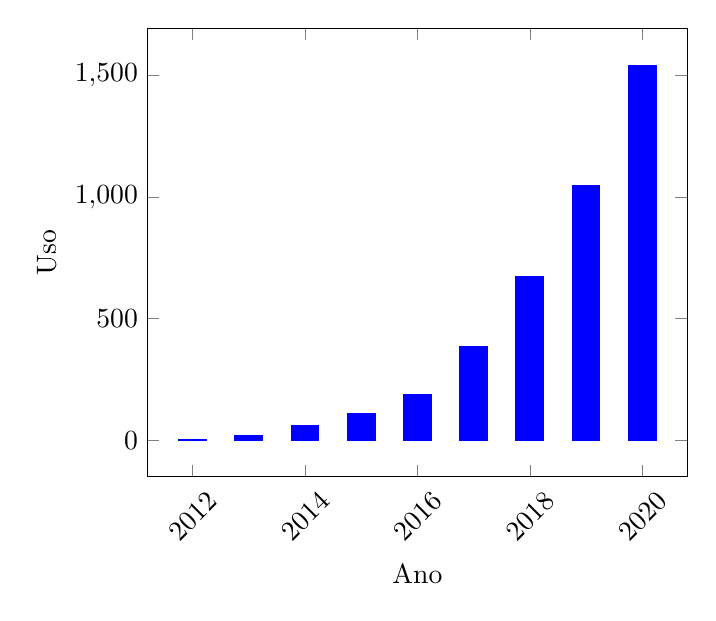
\begin{tikzpicture}[ybar]
		\begin{axis}[
				xlabel=Ano,ylabel=Uso,
				x tick label style={rotate=45, /pgf/number format/.cd,
						scaled x ticks = false,
						set thousands separator={},
						fixed}]
			\addplot [draw=blue, fill=blue] coordinates {
					(2012, 6)
					(2013, 19)
					(2014, 62)
					(2015, 113)
					(2016, 189)
					(2017, 387)
					(2018, 671)
					(2019, 1045)
					(2020, 1538)
				};
		\end{axis}
	\end{tikzpicture}
\end{frame}

\begin{frame}{\href{https://mc-stan.org}{\texttt{Stan}}\footnote{baseado no \href{https://breckbaldwin.github.io/ScientificSoftwareImpactMetrics/DeepLearningAndBayesianSoftware.html}{reporte anual do Breck Baldwin para a NUMFocus}}\footnote{veja as buscas Scopus nos \hyperlink{appendixscopus}{Slides de Backup no final dessa apresentação}}}
	\centering
	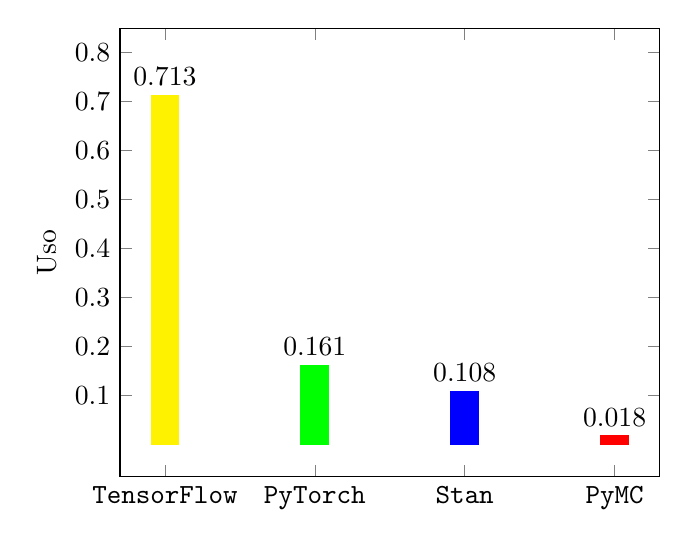
\begin{tikzpicture}[ybar]
		\begin{axis}[
				nodes near coords={\pgfmathprintnumber[fixed,precision=3]{\pgfplotspointmeta}},
				ylabel=Uso, xtick={1,2,3,4},
				ymax=0.85,
				ytick={0.1, 0.2, 0.3, 0.4, 0.5, 0.6, 0.7, 0.8},
				xticklabels={\texttt{TensorFlow}, \texttt{PyTorch}, \texttt{Stan}, \texttt{PyMC}}]
			\addplot [draw=yellow, fill=yellow] coordinates {
					(1, 0.713)};
			\addplot [draw=green, fill=green] coordinates {
					(2, 0.161)};
			\addplot [draw=blue, fill=blue] coordinates {
					(3, 0.108)};
			\addplot [draw=red, fill=red] coordinates {
					(4, 0.0176)};
		\end{axis}
	\end{tikzpicture}
\end{frame}

\subsection{Especificação de Modelos com Fórmulas}
\begin{frame}[fragile]{Especificação de Modelos com Fórmulas}
	Todos os modelos especificados pelo \href{http://mc-stan.org/rstanarm/}{\texttt{rstanarm}}
	e \href{https://paul-buerkner.github.io/brms/}{\texttt{brms}} usam uma fórmula
	com a seguinte síntaxe:
	\vfill
	\begin{lstlisting}
    dependente ~ independente_1 + independente_2 + ...
    \end{lstlisting}
\end{frame}

\begin{frame}[fragile]{Especificação de Modelos com Fórmulas}
	Moderações?! Sem problema:
	\vfill
	\begin{lstlisting}[basicstyle=\footnotesize]
dependente ~ independente_1 * moderadora + independente_2 * moderadora + ...
    \end{lstlisting}
\end{frame}

\subsection{Funções de Verossimilhança com \texttt{family}}
\begin{frame}{Funções de Verossimilhança com \texttt{family}}
	Todo modelo especificado pelo \href{http://mc-stan.org/rstanarm/}{\texttt{rstanarm}} e
	\href{https://paul-buerkner.github.io/brms/}{\texttt{brms}} devem especificar qual
	família da função de verossimilhança (\texttt{family}) respectivamente com a
	função de ligação (\texttt{link}) que fará o mapeamento dos parâmetros
	condicionados nos dados para a variável
	dependente\footnote{caso o usuário não designe nenhum valor para esses dois parâmetros, \href{http://mc-stan.org/rstanarm/}{\texttt{rstanarm}} e \href{https://paul-buerkner.github.io/brms/}{\texttt{brms}} usarão a verossimilhança Gaussiana (\texttt{family = gaussian}) e a função de identidade como função de ligação (\texttt{link = "identity"})}.
\end{frame}

\begin{frame}{Funções de Verossimilhança com \texttt{family}}
	\begin{vfilleditems}
		\item Gaussiana -- \texttt{family = gaussian(link = "identity")}
		\item Log-Normal -- \texttt{family = lognormal(link = "log")}
		\item Binomial -- \texttt{family = binomial(link = "logit")}
		\item Poisson -- \texttt{family = poisson(link = "log")}
		\item Binomial Negativa -- \texttt{family = negbinomial(link = "log")}
		\item $t$ de Student -- \texttt{family = student(link = "identity")}
		\item Exponencial -- \texttt{family = exponential(link = "log")}
	\end{vfilleditems}
\end{frame}

\subsection{\texttt{rstanarm}}

\begin{frame}{\href{http://mc-stan.org/rstanarm/}{\texttt{rstanarm}}\footnote{\textcite{rstanarm}}}
	O \href{http://mc-stan.org/rstanarm/}{\texttt{rstanarm}} é a porta de
	entrada para estatística Bayesiana com \href{https://mc-stan.org}{\texttt{Stan}}.
	\vfill
	O nome \texttt{rstanarm} é:
	\begin{vfilleditems}
		\item \texttt{r}: pacote para \texttt{R}
		\item \texttt{stan}: usa a linguagem probabilística \texttt{Stan}
		\item \texttt{arm}: acrônimo para \textit{Applied Regression Modeling}
	\end{vfilleditems}
\end{frame}

\subsubsection{Modelos do \texttt{rstanarm}}
\begin{frame}{Modelos do \href{http://mc-stan.org/rstanarm/}{\texttt{rstanarm}}\footnote{Neste curso usaremos apenas \texttt{stan\_glm} e \texttt{stan\_glmer}, mas saiba que você possui uma vasta categoria de modelos Bayesianos à disposição}}
	\begin{vfilleditems}
		\item \texttt{stan\_glm()} -- modelos lineares generalizados (\textit{\textbf{g}eneralized \textbf{l}inear \textbf{m}odel})
		\item \texttt{stan\_lm()} -- modelos lineares regularizados (\textit{\textbf{l}inear \textbf{m}odel)}
		\item \texttt{stan\_aov()} -- modelo ANOVA (\textit{\textbf{an}alysis \textbf{o}f \textbf{va}riance})
		\item \texttt{stan\_glmer()} - modelos linares generalizados multiníveis
		\item \texttt{stan\_lmer()} -- modelos linares regularizados multiníveis
		\item \texttt{stan\_jm()} -- modelos longitudinais e de sobrevivência
		\item \texttt{stan\_nlmer()} -- modelos não-lineares multiníveis (\textit{\textbf{n}on-\textbf{l}inear \textbf{m}odel})
		\item \texttt{stan\_polr()} -- modelos ordinais
		\item \texttt{stan\_gamm4()} -- modelos aditivos linares multiníveis
	\end{vfilleditems}
\end{frame}

\begin{frame}[fragile]{Exemplo Simples do \href{http://mc-stan.org/rstanarm/}{\texttt{rstanarm}}}
	\begin{lstlisting}
    library(rstanarm)
    rstanarm_fit <- @stan_glm(mpg ~ wt + am, data = mtcars)@
    summary(rstanarm_fit)
    \end{lstlisting}
\end{frame}

\begin{frame}{\texttt{summary} do \href{http://mc-stan.org/rstanarm/}{\texttt{rstanarm}}}
	\centering
	\begin{tabular}{lrrrrrrr}
		\toprule
		Parameter   & Rhat & n\_eff & mean  & sd   & 2.5\% & 50\%  & 97.5\% \\
		\midrule
		(Intercept) & 1.00 & 2157   & 37.16 & 3.20 & 30.78 & 37.16 & 43.44  \\
		wt          & 1.00 & 2285   & -5.32 & 0.83 & -6.91 & -5.32 & -3.65  \\
		am          & 1.00 & 2263   & 0.07  & 1.62 & -3.11 & 0.07  & 3.15   \\
		\bottomrule
	\end{tabular}
\end{frame}

\subsubsection{Visualizações do \texttt{rstanarm}}
\begin{frame}{Visualizações do \href{http://mc-stan.org/rstanarm/}{\texttt{rstanarm}}}
	% rstanarm_fit <- stan_glm(mpg ~ wt + am, data = mtcars)
	% library(ggplot2)
	% library(ggdark)
	% library(bayesplot)
	% library(tikzDevice)
	% theme_set(dark_theme_light())
	% bayesplot_theme_set(dark_theme_light())
	% tikz(file = "slides/images/mcmc_areas.tex")
	% mcmc_dens(rstanarm_fit)
	% dev.off()
	\centering
	\begin{figure}
		\resizebox{.45\linewidth}{!}{% Created by tikzDevice version 0.12.3.1 on 2021-05-28 14:47:20
% !TEX encoding = UTF-8 Unicode
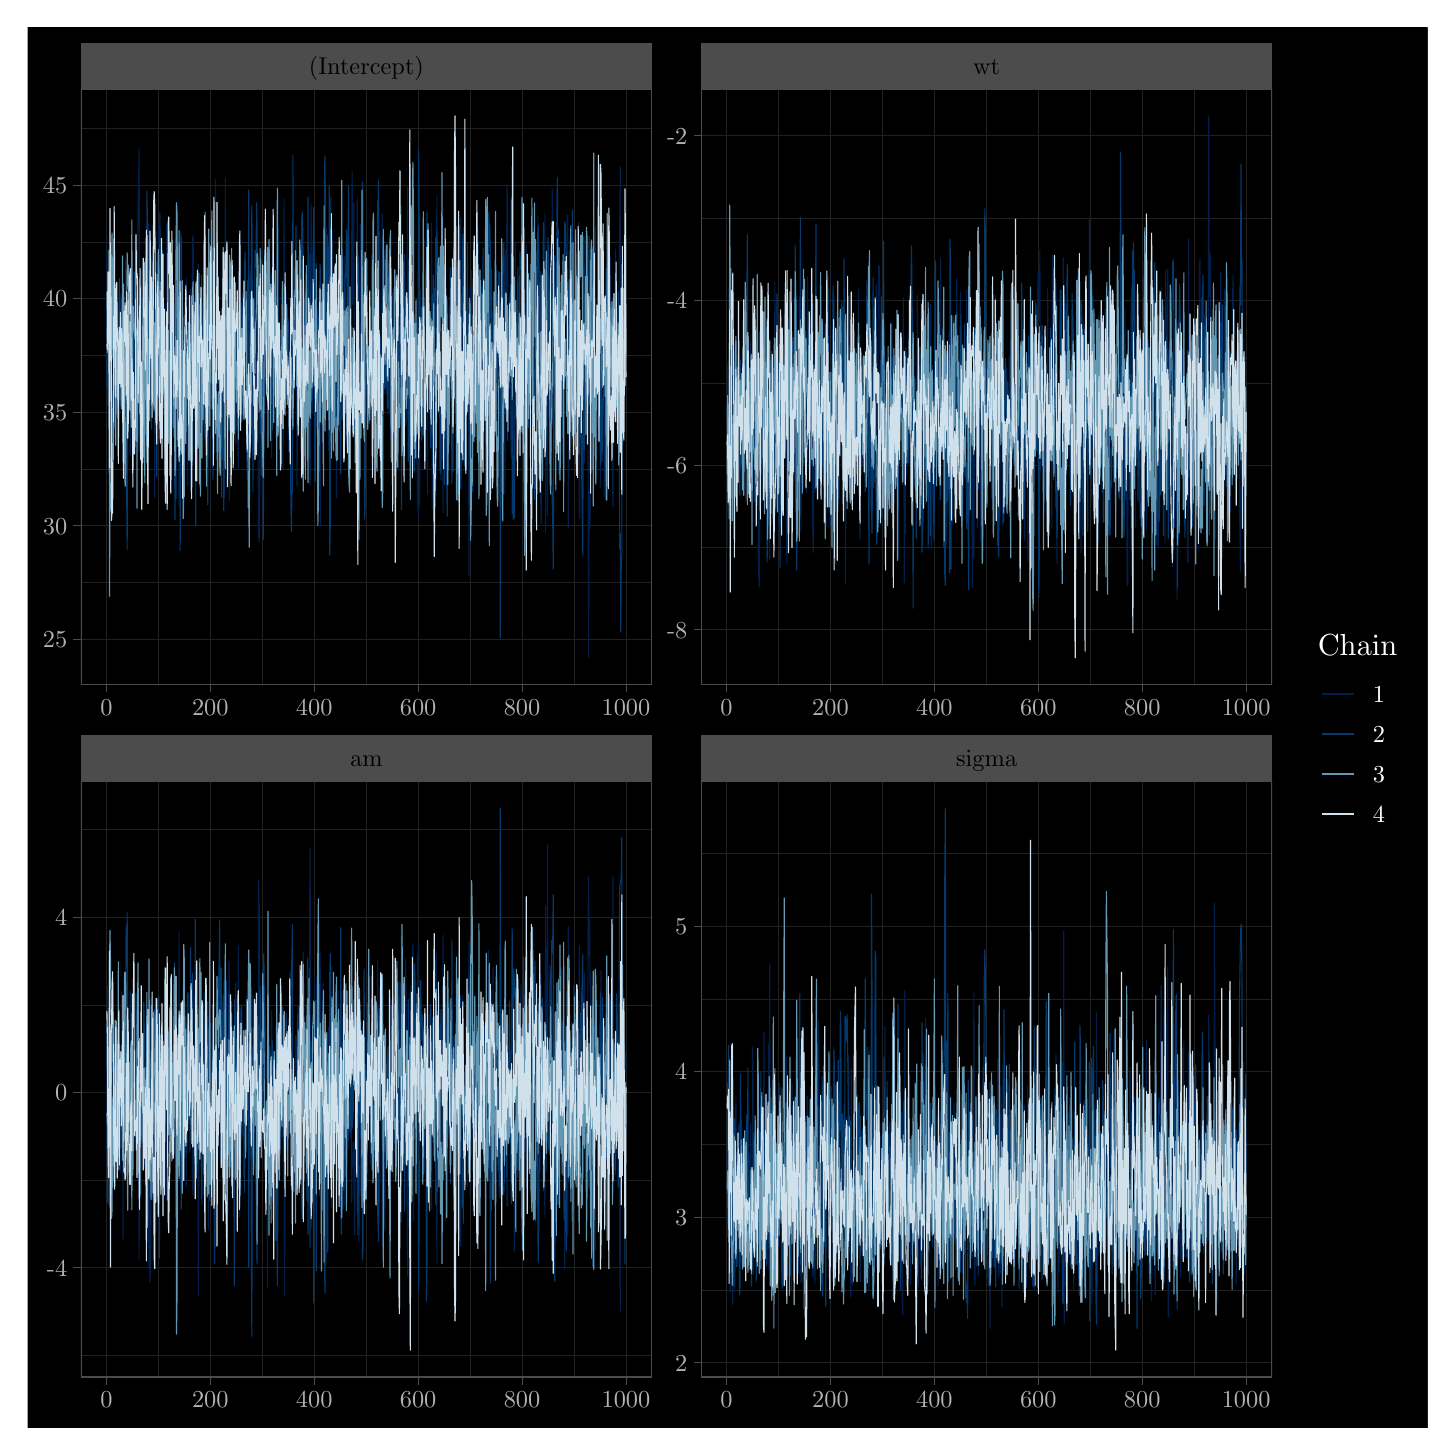
\begin{tikzpicture}[x=1pt,y=1pt]
\definecolor{fillColor}{RGB}{255,255,255}
\path[use as bounding box,fill=fillColor,fill opacity=0.00] (0,0) rectangle (505.89,505.89);
\begin{scope}
\path[clip] (  0.00,  0.00) rectangle (505.89,505.89);
\definecolor{drawColor}{RGB}{0,0,0}
\definecolor{fillColor}{RGB}{0,0,0}

\path[draw=drawColor,line width= 0.6pt,line join=round,line cap=round,fill=fillColor] (  0.00,  0.00) rectangle (505.89,505.89);
\end{scope}
\begin{scope}
\path[clip] ( 19.25,268.42) rectangle (225.57,483.82);
\definecolor{fillColor}{RGB}{0,0,0}

\path[fill=fillColor] ( 19.25,268.42) rectangle (225.57,483.82);
\definecolor{drawColor}{gray}{0.13}

\path[draw=drawColor,line width= 0.1pt,line join=round] ( 19.25,305.41) --
	(225.57,305.41);

\path[draw=drawColor,line width= 0.1pt,line join=round] ( 19.25,346.45) --
	(225.57,346.45);

\path[draw=drawColor,line width= 0.1pt,line join=round] ( 19.25,387.50) --
	(225.57,387.50);

\path[draw=drawColor,line width= 0.1pt,line join=round] ( 19.25,428.54) --
	(225.57,428.54);

\path[draw=drawColor,line width= 0.1pt,line join=round] ( 19.25,469.58) --
	(225.57,469.58);

\path[draw=drawColor,line width= 0.1pt,line join=round] ( 47.21,268.42) --
	( 47.21,483.82);

\path[draw=drawColor,line width= 0.1pt,line join=round] ( 84.76,268.42) --
	( 84.76,483.82);

\path[draw=drawColor,line width= 0.1pt,line join=round] (122.32,268.42) --
	(122.32,483.82);

\path[draw=drawColor,line width= 0.1pt,line join=round] (159.87,268.42) --
	(159.87,483.82);

\path[draw=drawColor,line width= 0.1pt,line join=round] (197.42,268.42) --
	(197.42,483.82);

\path[draw=drawColor,line width= 0.3pt,line join=round] ( 19.25,284.89) --
	(225.57,284.89);

\path[draw=drawColor,line width= 0.3pt,line join=round] ( 19.25,325.93) --
	(225.57,325.93);

\path[draw=drawColor,line width= 0.3pt,line join=round] ( 19.25,366.97) --
	(225.57,366.97);

\path[draw=drawColor,line width= 0.3pt,line join=round] ( 19.25,408.02) --
	(225.57,408.02);

\path[draw=drawColor,line width= 0.3pt,line join=round] ( 19.25,449.06) --
	(225.57,449.06);

\path[draw=drawColor,line width= 0.3pt,line join=round] ( 28.44,268.42) --
	( 28.44,483.82);

\path[draw=drawColor,line width= 0.3pt,line join=round] ( 65.99,268.42) --
	( 65.99,483.82);

\path[draw=drawColor,line width= 0.3pt,line join=round] (103.54,268.42) --
	(103.54,483.82);

\path[draw=drawColor,line width= 0.3pt,line join=round] (141.09,268.42) --
	(141.09,483.82);

\path[draw=drawColor,line width= 0.3pt,line join=round] (178.64,268.42) --
	(178.64,483.82);

\path[draw=drawColor,line width= 0.3pt,line join=round] (216.19,268.42) --
	(216.19,483.82);
\definecolor{drawColor}{RGB}{1,31,75}

\path[draw=drawColor,line width= 0.4pt,line join=round] ( 28.63,430.43) --
	( 28.81,369.22) --
	( 29.00,371.74) --
	( 29.19,410.83) --
	( 29.38,387.06) --
	( 29.56,360.28) --
	( 29.75,394.63) --
	( 29.94,394.63) --
	( 30.13,405.44) --
	( 30.32,389.46) --
	( 30.50,388.32) --
	( 30.69,407.90) --
	( 30.88,422.18) --
	( 31.07,404.40) --
	( 31.25,378.74) --
	( 31.44,361.23) --
	( 31.63,394.02) --
	( 31.82,399.99) --
	( 32.01,379.65) --
	( 32.19,400.26) --
	( 32.38,364.90) --
	( 32.57,367.34) --
	( 32.76,386.45) --
	( 32.94,365.27) --
	( 33.13,390.36) --
	( 33.32,393.73) --
	( 33.51,404.27) --
	( 33.70,409.80) --
	( 33.88,387.51) --
	( 34.07,369.23) --
	( 34.26,403.85) --
	( 34.45,407.49) --
	( 34.63,384.12) --
	( 34.82,389.71) --
	( 35.01,358.33) --
	( 35.20,389.82) --
	( 35.39,422.02) --
	( 35.57,384.98) --
	( 35.76,391.02) --
	( 35.95,395.66) --
	( 36.14,391.43) --
	( 36.32,390.91) --
	( 36.51,396.42) --
	( 36.70,376.97) --
	( 36.89,392.23) --
	( 37.08,351.77) --
	( 37.26,373.58) --
	( 37.45,422.34) --
	( 37.64,392.41) --
	( 37.83,369.08) --
	( 38.01,370.65) --
	( 38.20,386.14) --
	( 38.39,372.96) --
	( 38.58,373.13) --
	( 38.76,411.10) --
	( 38.95,360.45) --
	( 39.14,378.42) --
	( 39.33,364.24) --
	( 39.52,364.30) --
	( 39.70,407.10) --
	( 39.89,443.24) --
	( 40.08,448.60) --
	( 40.27,462.37) --
	( 40.45,384.28) --
	( 40.64,386.75) --
	( 40.83,378.59) --
	( 41.02,352.94) --
	( 41.21,418.03) --
	( 41.39,374.70) --
	( 41.58,397.70) --
	( 41.77,385.36) --
	( 41.96,391.40) --
	( 42.14,393.14) --
	( 42.33,401.16) --
	( 42.52,406.34) --
	( 42.71,425.25) --
	( 42.90,409.06) --
	( 43.08,357.06) --
	( 43.27,389.61) --
	( 43.46,395.38) --
	( 43.65,435.10) --
	( 43.83,421.87) --
	( 44.02,430.73) --
	( 44.21,431.06) --
	( 44.40,421.58) --
	( 44.59,422.06) --
	( 44.77,378.63) --
	( 44.96,376.64) --
	( 45.15,378.40) --
	( 45.34,375.98) --
	( 45.52,408.02) --
	( 45.71,411.12) --
	( 45.90,336.22) --
	( 46.09,405.91) --
	( 46.28,432.19) --
	( 46.46,394.45) --
	( 46.65,383.04) --
	( 46.84,421.39) --
	( 47.03,398.25) --
	( 47.21,403.52) --
	( 47.40,435.46) --
	( 47.59,366.52) --
	( 47.78,397.08) --
	( 47.96,402.08) --
	( 48.15,388.35) --
	( 48.34,383.20) --
	( 48.53,392.52) --
	( 48.72,382.26) --
	( 48.90,382.20) --
	( 49.09,399.77) --
	( 49.28,406.02) --
	( 49.47,372.24) --
	( 49.65,376.41) --
	( 49.84,374.15) --
	( 50.03,372.07) --
	( 50.22,434.71) --
	( 50.41,387.18) --
	( 50.59,369.09) --
	( 50.78,378.77) --
	( 50.97,386.91) --
	( 51.16,373.43) --
	( 51.34,370.81) --
	( 51.53,386.53) --
	( 51.72,363.13) --
	( 51.91,372.73) --
	( 52.10,391.75) --
	( 52.28,371.30) --
	( 52.47,407.16) --
	( 52.66,387.58) --
	( 52.85,405.43) --
	( 53.03,358.73) --
	( 53.22,376.10) --
	( 53.41,429.52) --
	( 53.60,429.75) --
	( 53.79,383.15) --
	( 53.97,396.75) --
	( 54.16,381.66) --
	( 54.35,391.80) --
	( 54.54,361.17) --
	( 54.72,332.65) --
	( 54.91,422.37) --
	( 55.10,376.91) --
	( 55.29,432.10) --
	( 55.47,420.81) --
	( 55.66,368.72) --
	( 55.85,364.10) --
	( 56.04,373.63) --
	( 56.23,392.79) --
	( 56.41,329.47) --
	( 56.60,348.81) --
	( 56.79,393.32) --
	( 56.98,380.19) --
	( 57.16,377.76) --
	( 57.35,415.39) --
	( 57.54,358.06) --
	( 57.73,340.33) --
	( 57.92,391.02) --
	( 58.10,394.73) --
	( 58.29,350.59) --
	( 58.48,406.57) --
	( 58.67,402.16) --
	( 58.85,411.28) --
	( 59.04,345.28) --
	( 59.23,377.51) --
	( 59.42,409.97) --
	( 59.61,429.60) --
	( 59.79,430.93) --
	( 59.98,388.72) --
	( 60.17,405.42) --
	( 60.36,408.11) --
	( 60.54,390.55) --
	( 60.73,383.58) --
	( 60.92,391.37) --
	( 61.11,351.99) --
	( 61.30,370.45) --
	( 61.48,419.95) --
	( 61.67,420.32) --
	( 61.86,407.65) --
	( 62.05,357.25) --
	( 62.23,399.21) --
	( 62.42,367.40) --
	( 62.61,382.69) --
	( 62.80,381.91) --
	( 62.99,405.02) --
	( 63.17,391.96) --
	( 63.36,374.63) --
	( 63.55,408.00) --
	( 63.74,360.06) --
	( 63.92,418.92) --
	( 64.11,388.63) --
	( 64.30,403.80) --
	( 64.49,394.19) --
	( 64.67,386.23) --
	( 64.86,362.81) --
	( 65.05,365.90) --
	( 65.24,394.57) --
	( 65.43,426.07) --
	( 65.61,378.05) --
	( 65.80,379.73) --
	( 65.99,374.26) --
	( 66.18,375.99) --
	( 66.36,396.72) --
	( 66.55,375.71) --
	( 66.74,365.77) --
	( 66.93,354.14) --
	( 67.12,360.08) --
	( 67.30,356.33) --
	( 67.49,399.20) --
	( 67.68,393.18) --
	( 67.87,450.94) --
	( 68.05,423.47) --
	( 68.24,369.63) --
	( 68.43,384.61) --
	( 68.62,416.72) --
	( 68.81,408.93) --
	( 68.99,391.32) --
	( 69.18,403.02) --
	( 69.37,363.06) --
	( 69.56,358.41) --
	( 69.74,390.25) --
	( 69.93,396.53) --
	( 70.12,397.39) --
	( 70.31,393.12) --
	( 70.50,408.03) --
	( 70.68,417.84) --
	( 70.87,399.92) --
	( 71.06,338.27) --
	( 71.25,352.87) --
	( 71.43,451.67) --
	( 71.62,380.39) --
	( 71.81,389.94) --
	( 72.00,378.38) --
	( 72.19,388.09) --
	( 72.37,414.82) --
	( 72.56,391.82) --
	( 72.75,343.52) --
	( 72.94,334.97) --
	( 73.12,405.53) --
	( 73.31,395.11) --
	( 73.50,361.35) --
	( 73.69,374.37) --
	( 73.87,363.60) --
	( 74.06,401.47) --
	( 74.25,396.79) --
	( 74.44,410.39) --
	( 74.63,367.78) --
	( 74.81,392.17) --
	( 75.00,382.98) --
	( 75.19,355.46) --
	( 75.38,368.45) --
	( 75.56,390.95) --
	( 75.75,365.00) --
	( 75.94,354.88) --
	( 76.13,346.07) --
	( 76.32,393.03) --
	( 76.50,428.95) --
	( 76.69,432.88) --
	( 76.88,388.07) --
	( 77.07,366.59) --
	( 77.25,364.48) --
	( 77.44,394.11) --
	( 77.63,410.04) --
	( 77.82,371.46) --
	( 78.01,409.49) --
	( 78.19,391.56) --
	( 78.38,400.97) --
	( 78.57,395.66) --
	( 78.76,373.91) --
	( 78.94,382.63) --
	( 79.13,348.82) --
	( 79.32,342.59) --
	( 79.51,343.76) --
	( 79.70,341.94) --
	( 79.88,410.53) --
	( 80.07,348.10) --
	( 80.26,385.33) --
	( 80.45,402.53) --
	( 80.63,418.30) --
	( 80.82,373.20) --
	( 81.01,392.87) --
	( 81.20,410.79) --
	( 81.39,383.69) --
	( 81.57,351.76) --
	( 81.76,360.51) --
	( 81.95,396.97) --
	( 82.14,372.48) --
	( 82.32,376.28) --
	( 82.51,350.45) --
	( 82.70,404.80) --
	( 82.89,388.24) --
	( 83.07,384.82) --
	( 83.26,353.22) --
	( 83.45,322.29) --
	( 83.64,320.11) --
	( 83.83,333.23) --
	( 84.01,395.53) --
	( 84.20,397.06) --
	( 84.39,389.24) --
	( 84.58,387.98) --
	( 84.76,389.43) --
	( 84.95,378.09) --
	( 85.14,370.09) --
	( 85.33,367.95) --
	( 85.52,417.45) --
	( 85.70,384.79) --
	( 85.89,407.69) --
	( 86.08,402.84) --
	( 86.27,390.10) --
	( 86.45,381.89) --
	( 86.64,422.29) --
	( 86.83,408.25) --
	( 87.02,400.31) --
	( 87.21,397.25) --
	( 87.39,396.90) --
	( 87.58,404.01) --
	( 87.77,399.08) --
	( 87.96,417.43) --
	( 88.14,350.67) --
	( 88.33,381.71) --
	( 88.52,424.43) --
	( 88.71,397.13) --
	( 88.90,386.44) --
	( 89.08,397.17) --
	( 89.27,403.00) --
	( 89.46,389.42) --
	( 89.65,375.51) --
	( 89.83,363.97) --
	( 90.02,381.71) --
	( 90.21,389.79) --
	( 90.40,389.56) --
	( 90.58,381.81) --
	( 90.77,383.38) --
	( 90.96,368.89) --
	( 91.15,365.41) --
	( 91.34,396.70) --
	( 91.52,392.48) --
	( 91.71,389.97) --
	( 91.90,405.21) --
	( 92.09,399.34) --
	( 92.27,346.55) --
	( 92.46,373.42) --
	( 92.65,444.07) --
	( 92.84,385.40) --
	( 93.03,417.89) --
	( 93.21,385.96) --
	( 93.40,410.21) --
	( 93.59,403.93) --
	( 93.78,373.17) --
	( 93.96,396.11) --
	( 94.15,400.94) --
	( 94.34,352.77) --
	( 94.53,353.49) --
	( 94.72,357.40) --
	( 94.90,367.60) --
	( 95.09,370.56) --
	( 95.28,414.70) --
	( 95.47,418.62) --
	( 95.65,413.76) --
	( 95.84,415.23) --
	( 96.03,400.83) --
	( 96.22,387.04) --
	( 96.41,410.94) --
	( 96.59,388.35) --
	( 96.78,386.65) --
	( 96.97,386.59) --
	( 97.16,380.73) --
	( 97.34,340.06) --
	( 97.53,360.28) --
	( 97.72,378.22) --
	( 97.91,388.09) --
	( 98.10,384.80) --
	( 98.28,400.61) --
	( 98.47,423.68) --
	( 98.66,382.40) --
	( 98.85,370.60) --
	( 99.03,414.22) --
	( 99.22,342.54) --
	( 99.41,370.46) --
	( 99.60,348.41) --
	( 99.78,382.96) --
	( 99.97,377.37) --
	(100.16,378.15) --
	(100.35,411.98) --
	(100.54,406.54) --
	(100.72,378.22) --
	(100.91,378.31) --
	(101.10,374.08) --
	(101.29,372.38) --
	(101.47,380.44) --
	(101.66,386.72) --
	(101.85,340.57) --
	(102.04,341.15) --
	(102.23,346.13) --
	(102.41,442.08) --
	(102.60,435.26) --
	(102.79,366.83) --
	(102.98,386.17) --
	(103.16,424.37) --
	(103.35,430.72) --
	(103.54,401.59) --
	(103.73,361.34) --
	(103.92,344.22) --
	(104.10,386.05) --
	(104.29,398.97) --
	(104.48,361.93) --
	(104.67,385.56) --
	(104.85,404.27) --
	(105.04,354.25) --
	(105.23,407.20) --
	(105.42,411.67) --
	(105.61,344.58) --
	(105.79,326.22) --
	(105.98,399.20) --
	(106.17,401.32) --
	(106.36,405.90) --
	(106.54,355.83) --
	(106.73,356.37) --
	(106.92,362.26) --
	(107.11,376.88) --
	(107.30,378.92) --
	(107.48,369.28) --
	(107.67,423.36) --
	(107.86,415.00) --
	(108.05,433.51) --
	(108.23,397.94) --
	(108.42,410.13) --
	(108.61,386.54) --
	(108.80,353.07) --
	(108.98,389.61) --
	(109.17,400.34) --
	(109.36,411.74) --
	(109.55,412.82) --
	(109.74,427.19) --
	(109.92,359.76) --
	(110.11,432.48) --
	(110.30,400.20) --
	(110.49,360.58) --
	(110.67,375.31) --
	(110.86,381.78) --
	(111.05,399.47) --
	(111.24,389.94) --
	(111.43,395.16) --
	(111.61,335.88) --
	(111.80,395.19) --
	(111.99,385.95) --
	(112.18,369.22) --
	(112.36,371.35) --
	(112.55,381.24) --
	(112.74,363.77) --
	(112.93,347.11) --
	(113.12,416.01) --
	(113.30,414.41) --
	(113.49,364.32) --
	(113.68,365.41) --
	(113.87,374.62) --
	(114.05,394.09) --
	(114.24,389.71) --
	(114.43,377.28) --
	(114.62,423.35) --
	(114.81,404.91) --
	(114.99,398.81) --
	(115.18,355.05) --
	(115.37,368.22) --
	(115.56,384.66) --
	(115.74,391.67) --
	(115.93,393.18) --
	(116.12,397.75) --
	(116.31,348.97) --
	(116.49,380.87) --
	(116.68,376.14) --
	(116.87,396.22) --
	(117.06,422.38) --
	(117.25,453.88) --
	(117.43,405.87) --
	(117.62,423.72) --
	(117.81,442.35) --
	(118.00,400.72) --
	(118.18,398.51) --
	(118.37,395.67) --
	(118.56,389.86) --
	(118.75,368.79) --
	(118.94,419.08) --
	(119.12,443.93) --
	(119.31,377.88) --
	(119.50,404.12) --
	(119.69,397.51) --
	(119.87,376.18) --
	(120.06,389.09) --
	(120.25,434.75) --
	(120.44,385.83) --
	(120.63,364.02) --
	(120.81,378.16) --
	(121.00,383.99) --
	(121.19,402.79) --
	(121.38,386.54) --
	(121.56,376.72) --
	(121.75,380.61) --
	(121.94,394.64) --
	(122.13,373.78) --
	(122.32,378.46) --
	(122.50,364.67) --
	(122.69,367.13) --
	(122.88,371.05) --
	(123.07,382.03) --
	(123.25,375.74) --
	(123.44,376.05) --
	(123.63,385.22) --
	(123.82,398.76) --
	(124.01,390.80) --
	(124.19,382.73) --
	(124.38,419.03) --
	(124.57,395.65) --
	(124.76,398.65) --
	(124.94,374.18) --
	(125.13,385.30) --
	(125.32,392.37) --
	(125.51,400.15) --
	(125.69,341.93) --
	(125.88,378.84) --
	(126.07,366.82) --
	(126.26,401.70) --
	(126.45,354.71) --
	(126.63,361.14) --
	(126.82,370.63) --
	(127.01,402.90) --
	(127.20,432.22) --
	(127.38,388.95) --
	(127.57,390.23) --
	(127.76,369.97) --
	(127.95,364.92) --
	(128.14,438.66) --
	(128.32,424.29) --
	(128.51,426.71) --
	(128.70,428.91) --
	(128.89,418.53) --
	(129.07,420.09) --
	(129.26,403.87) --
	(129.45,394.34) --
	(129.64,373.39) --
	(129.83,391.11) --
	(130.01,394.10) --
	(130.20,395.52) --
	(130.39,417.76) --
	(130.58,366.63) --
	(130.76,406.00) --
	(130.95,397.73) --
	(131.14,357.40) --
	(131.33,384.73) --
	(131.52,391.55) --
	(131.70,380.64) --
	(131.89,410.09) --
	(132.08,407.68) --
	(132.27,401.89) --
	(132.45,395.71) --
	(132.64,400.95) --
	(132.83,411.05) --
	(133.02,410.21) --
	(133.21,345.81) --
	(133.39,399.90) --
	(133.58,387.01) --
	(133.77,427.71) --
	(133.96,361.29) --
	(134.14,422.06) --
	(134.33,422.58) --
	(134.52,391.00) --
	(134.71,362.59) --
	(134.89,365.63) --
	(135.08,388.35) --
	(135.27,400.55) --
	(135.46,383.31) --
	(135.65,408.75) --
	(135.83,381.81) --
	(136.02,415.72) --
	(136.21,423.92) --
	(136.40,384.50) --
	(136.58,361.76) --
	(136.77,363.92) --
	(136.96,391.68) --
	(137.15,424.25) --
	(137.34,448.35) --
	(137.52,381.29) --
	(137.71,374.87) --
	(137.90,403.42) --
	(138.09,388.01) --
	(138.27,378.87) --
	(138.46,347.70) --
	(138.65,372.95) --
	(138.84,407.20) --
	(139.03,344.03) --
	(139.21,355.76) --
	(139.40,401.17) --
	(139.59,401.09) --
	(139.78,381.24) --
	(139.96,376.91) --
	(140.15,395.36) --
	(140.34,377.80) --
	(140.53,348.91) --
	(140.72,351.75) --
	(140.90,335.26) --
	(141.09,331.44) --
	(141.28,329.78) --
	(141.47,356.15) --
	(141.65,333.33) --
	(141.84,411.14) --
	(142.03,387.63) --
	(142.22,384.78) --
	(142.40,380.59) --
	(142.59,400.61) --
	(142.78,406.43) --
	(142.97,394.81) --
	(143.16,406.59) --
	(143.34,395.41) --
	(143.53,394.75) --
	(143.72,393.43) --
	(143.91,369.61) --
	(144.09,411.66) --
	(144.28,353.89) --
	(144.47,337.38) --
	(144.66,406.27) --
	(144.85,396.43) --
	(145.03,394.27) --
	(145.22,381.94) --
	(145.41,383.05) --
	(145.60,397.72) --
	(145.78,378.41) --
	(145.97,435.28) --
	(146.16,331.84) --
	(146.35,395.24) --
	(146.54,363.14) --
	(146.72,371.19) --
	(146.91,352.37) --
	(147.10,390.36) --
	(147.29,341.50) --
	(147.47,336.74) --
	(147.66,346.73) --
	(147.85,445.45) --
	(148.04,391.69) --
	(148.23,408.59) --
	(148.41,413.65) --
	(148.60,380.87) --
	(148.79,381.12) --
	(148.98,378.56) --
	(149.16,374.47) --
	(149.35,342.48) --
	(149.54,380.37) --
	(149.73,404.96) --
	(149.92,416.41) --
	(150.10,330.80) --
	(150.29,373.92) --
	(150.48,386.05) --
	(150.67,375.72) --
	(150.85,350.30) --
	(151.04,420.09) --
	(151.23,392.03) --
	(151.42,399.91) --
	(151.60,387.72) --
	(151.79,395.53) --
	(151.98,392.81) --
	(152.17,388.19) --
	(152.36,405.23) --
	(152.54,373.97) --
	(152.73,378.77) --
	(152.92,378.73) --
	(153.11,390.85) --
	(153.29,388.93) --
	(153.48,364.54) --
	(153.67,370.15) --
	(153.86,383.28) --
	(154.05,370.48) --
	(154.23,385.36) --
	(154.42,385.77) --
	(154.61,366.76) --
	(154.80,419.13) --
	(154.98,418.04) --
	(155.17,377.18) --
	(155.36,381.02) --
	(155.55,410.17) --
	(155.74,361.05) --
	(155.92,403.89) --
	(156.11,404.18) --
	(156.30,408.25) --
	(156.49,437.35) --
	(156.67,398.24) --
	(156.86,403.25) --
	(157.05,398.80) --
	(157.24,348.77) --
	(157.43,409.64) --
	(157.61,393.23) --
	(157.80,383.52) --
	(157.99,390.07) --
	(158.18,369.93) --
	(158.36,367.52) --
	(158.55,371.72) --
	(158.74,371.83) --
	(158.93,396.61) --
	(159.12,402.50) --
	(159.30,362.47) --
	(159.49,307.92) --
	(159.68,389.23) --
	(159.87,412.15) --
	(160.05,358.44) --
	(160.24,395.03) --
	(160.43,418.03) --
	(160.62,352.26) --
	(160.80,350.89) --
	(160.99,354.80) --
	(161.18,404.65) --
	(161.37,391.41) --
	(161.56,394.86) --
	(161.74,383.48) --
	(161.93,374.25) --
	(162.12,399.48) --
	(162.31,382.06) --
	(162.49,376.10) --
	(162.68,369.07) --
	(162.87,353.76) --
	(163.06,369.50) --
	(163.25,403.38) --
	(163.43,405.64) --
	(163.62,406.17) --
	(163.81,367.54) --
	(164.00,350.76) --
	(164.18,388.96) --
	(164.37,400.03) --
	(164.56,405.47) --
	(164.75,389.65) --
	(164.94,389.97) --
	(165.12,384.86) --
	(165.31,356.17) --
	(165.50,406.25) --
	(165.69,377.54) --
	(165.87,379.03) --
	(166.06,377.06) --
	(166.25,380.70) --
	(166.44,338.44) --
	(166.63,351.19) --
	(166.81,402.68) --
	(167.00,388.67) --
	(167.19,410.73) --
	(167.38,374.35) --
	(167.56,365.48) --
	(167.75,373.73) --
	(167.94,403.20) --
	(168.13,343.80) --
	(168.31,394.33) --
	(168.50,377.40) --
	(168.69,386.41) --
	(168.88,364.98) --
	(169.07,419.04) --
	(169.25,380.17) --
	(169.44,397.27) --
	(169.63,402.45) --
	(169.82,395.03) --
	(170.00,383.52) --
	(170.19,380.08) --
	(170.38,386.30) --
	(170.57,410.14) --
	(170.76,402.64) --
	(170.94,392.46) --
	(171.13,400.10) --
	(171.32,395.63) --
	(171.51,404.00) --
	(171.69,363.08) --
	(171.88,382.31) --
	(172.07,408.68) --
	(172.26,409.24) --
	(172.45,337.52) --
	(172.63,425.46) --
	(172.82,402.38) --
	(173.01,410.71) --
	(173.20,449.23) --
	(173.38,443.72) --
	(173.57,391.61) --
	(173.76,382.94) --
	(173.95,386.65) --
	(174.14,409.06) --
	(174.32,397.98) --
	(174.51,358.79) --
	(174.70,351.23) --
	(174.89,350.33) --
	(175.07,368.36) --
	(175.26,349.23) --
	(175.45,383.68) --
	(175.64,356.93) --
	(175.83,409.23) --
	(176.01,385.15) --
	(176.20,428.46) --
	(176.39,363.19) --
	(176.58,373.45) --
	(176.76,395.59) --
	(176.95,343.09) --
	(177.14,364.43) --
	(177.33,386.32) --
	(177.51,364.84) --
	(177.70,401.63) --
	(177.89,365.27) --
	(178.08,366.13) --
	(178.27,368.86) --
	(178.45,375.32) --
	(178.64,400.04) --
	(178.83,431.52) --
	(179.02,422.79) --
	(179.20,334.46) --
	(179.39,402.74) --
	(179.58,379.03) --
	(179.77,374.36) --
	(179.96,394.29) --
	(180.14,427.16) --
	(180.33,383.23) --
	(180.52,395.73) --
	(180.71,420.93) --
	(180.89,411.93) --
	(181.08,390.13) --
	(181.27,391.51) --
	(181.46,367.08) --
	(181.65,372.11) --
	(181.83,388.84) --
	(182.02,379.26) --
	(182.21,410.42) --
	(182.40,413.01) --
	(182.58,365.16) --
	(182.77,370.40) --
	(182.96,358.82) --
	(183.15,395.89) --
	(183.34,382.92) --
	(183.52,398.33) --
	(183.71,366.30) --
	(183.90,424.95) --
	(184.09,393.86) --
	(184.27,392.15) --
	(184.46,437.99) --
	(184.65,383.32) --
	(184.84,383.06) --
	(185.03,365.87) --
	(185.21,368.30) --
	(185.40,334.15) --
	(185.59,326.69) --
	(185.78,376.38) --
	(185.96,388.99) --
	(186.15,373.51) --
	(186.34,343.63) --
	(186.53,406.08) --
	(186.71,418.32) --
	(186.90,438.59) --
	(187.09,323.35) --
	(187.28,349.47) --
	(187.47,356.53) --
	(187.65,376.28) --
	(187.84,329.52) --
	(188.03,400.35) --
	(188.22,365.08) --
	(188.40,392.73) --
	(188.59,416.41) --
	(188.78,415.64) --
	(188.97,354.22) --
	(189.16,353.31) --
	(189.34,406.75) --
	(189.53,447.79) --
	(189.72,361.52) --
	(189.91,369.96) --
	(190.09,387.15) --
	(190.28,375.35) --
	(190.47,398.76) --
	(190.66,404.10) --
	(190.85,411.52) --
	(191.03,386.01) --
	(191.22,447.56) --
	(191.41,386.96) --
	(191.60,392.10) --
	(191.78,350.10) --
	(191.97,386.60) --
	(192.16,372.24) --
	(192.35,377.18) --
	(192.54,387.96) --
	(192.72,400.84) --
	(192.91,379.13) --
	(193.10,403.04) --
	(193.29,382.07) --
	(193.47,348.32) --
	(193.66,399.44) --
	(193.85,397.29) --
	(194.04,429.52) --
	(194.22,423.88) --
	(194.41,401.61) --
	(194.60,416.43) --
	(194.79,405.40) --
	(194.98,438.09) --
	(195.16,438.09) --
	(195.35,325.04) --
	(195.54,348.40) --
	(195.73,365.43) --
	(195.91,396.11) --
	(196.10,372.43) --
	(196.29,380.94) --
	(196.48,354.82) --
	(196.67,368.56) --
	(196.85,415.60) --
	(197.04,402.73) --
	(197.23,401.97) --
	(197.42,401.09) --
	(197.60,379.41) --
	(197.79,377.48) --
	(197.98,388.41) --
	(198.17,389.08) --
	(198.36,380.11) --
	(198.54,405.43) --
	(198.73,403.66) --
	(198.92,410.18) --
	(199.11,435.55) --
	(199.29,332.31) --
	(199.48,328.56) --
	(199.67,389.47) --
	(199.86,369.55) --
	(200.05,372.83) --
	(200.23,387.39) --
	(200.42,415.27) --
	(200.61,395.58) --
	(200.80,380.72) --
	(200.98,378.46) --
	(201.17,348.81) --
	(201.36,391.77) --
	(201.55,398.09) --
	(201.74,389.13) --
	(201.92,378.25) --
	(202.11,398.22) --
	(202.30,379.34) --
	(202.49,345.98) --
	(202.67,278.21) --
	(202.86,338.66) --
	(203.05,338.37) --
	(203.24,325.07) --
	(203.42,350.86) --
	(203.61,408.40) --
	(203.80,414.66) --
	(203.99,403.08) --
	(204.18,400.08) --
	(204.36,416.51) --
	(204.55,424.28) --
	(204.74,415.64) --
	(204.93,424.93) --
	(205.11,433.73) --
	(205.30,360.73) --
	(205.49,343.45) --
	(205.68,364.17) --
	(205.87,376.47) --
	(206.05,361.57) --
	(206.24,376.49) --
	(206.43,430.04) --
	(206.62,410.66) --
	(206.80,426.84) --
	(206.99,339.57) --
	(207.18,365.43) --
	(207.37,382.47) --
	(207.56,386.78) --
	(207.74,388.40) --
	(207.93,415.82) --
	(208.12,410.31) --
	(208.31,336.34) --
	(208.49,385.59) --
	(208.68,341.68) --
	(208.87,376.69) --
	(209.06,407.82) --
	(209.25,381.47) --
	(209.43,370.78) --
	(209.62,367.50) --
	(209.81,415.82) --
	(210.00,417.90) --
	(210.18,368.62) --
	(210.37,389.85) --
	(210.56,422.99) --
	(210.75,380.76) --
	(210.94,382.27) --
	(211.12,357.12) --
	(211.31,342.66) --
	(211.50,332.86) --
	(211.69,387.21) --
	(211.87,403.10) --
	(212.06,384.99) --
	(212.25,407.14) --
	(212.44,425.77) --
	(212.62,381.63) --
	(212.81,386.10) --
	(213.00,404.43) --
	(213.19,392.24) --
	(213.38,391.79) --
	(213.56,381.19) --
	(213.75,423.57) --
	(213.94,434.27) --
	(214.13,455.76) --
	(214.31,398.27) --
	(214.50,401.10) --
	(214.69,392.03) --
	(214.88,377.83) --
	(215.07,391.22) --
	(215.25,381.56) --
	(215.44,395.43) --
	(215.63,378.02) --
	(215.82,394.62) --
	(216.00,377.55) --
	(216.19,378.14);
\definecolor{drawColor}{RGB}{3,57,108}

\path[draw=drawColor,line width= 0.4pt,line join=round] ( 28.63,375.42) --
	( 28.81,411.30) --
	( 29.00,404.28) --
	( 29.19,415.58) --
	( 29.38,409.52) --
	( 29.56,422.26) --
	( 29.75,393.55) --
	( 29.94,419.91) --
	( 30.13,392.27) --
	( 30.32,405.44) --
	( 30.50,363.23) --
	( 30.69,347.25) --
	( 30.88,372.02) --
	( 31.07,375.44) --
	( 31.25,394.61) --
	( 31.44,406.40) --
	( 31.63,397.73) --
	( 31.82,369.69) --
	( 32.01,392.65) --
	( 32.19,403.72) --
	( 32.38,394.51) --
	( 32.57,384.94) --
	( 32.76,388.85) --
	( 32.94,399.18) --
	( 33.13,415.27) --
	( 33.32,372.73) --
	( 33.51,369.14) --
	( 33.70,396.12) --
	( 33.88,393.91) --
	( 34.07,390.57) --
	( 34.26,405.87) --
	( 34.45,387.35) --
	( 34.63,373.71) --
	( 34.82,365.68) --
	( 35.01,371.55) --
	( 35.20,396.04) --
	( 35.39,382.77) --
	( 35.57,360.37) --
	( 35.76,339.01) --
	( 35.95,317.36) --
	( 36.14,375.72) --
	( 36.32,402.04) --
	( 36.51,396.16) --
	( 36.70,387.44) --
	( 36.89,391.64) --
	( 37.08,391.86) --
	( 37.26,399.11) --
	( 37.45,383.23) --
	( 37.64,380.04) --
	( 37.83,382.72) --
	( 38.01,389.78) --
	( 38.20,365.64) --
	( 38.39,375.46) --
	( 38.58,417.53) --
	( 38.76,399.64) --
	( 38.95,394.85) --
	( 39.14,366.27) --
	( 39.33,372.59) --
	( 39.52,370.52) --
	( 39.70,389.19) --
	( 39.89,389.87) --
	( 40.08,389.75) --
	( 40.27,352.76) --
	( 40.45,390.13) --
	( 40.64,385.52) --
	( 40.83,404.21) --
	( 41.02,412.75) --
	( 41.21,380.61) --
	( 41.39,371.70) --
	( 41.58,407.87) --
	( 41.77,379.90) --
	( 41.96,348.73) --
	( 42.14,364.33) --
	( 42.33,372.93) --
	( 42.52,413.26) --
	( 42.71,376.04) --
	( 42.90,378.72) --
	( 43.08,446.81) --
	( 43.27,436.51) --
	( 43.46,413.32) --
	( 43.65,396.89) --
	( 43.83,397.13) --
	( 44.02,383.19) --
	( 44.21,382.63) --
	( 44.40,395.09) --
	( 44.59,364.93) --
	( 44.77,360.97) --
	( 44.96,397.60) --
	( 45.15,408.39) --
	( 45.34,380.42) --
	( 45.52,406.59) --
	( 45.71,385.40) --
	( 45.90,384.27) --
	( 46.09,379.27) --
	( 46.28,374.55) --
	( 46.46,397.68) --
	( 46.65,343.78) --
	( 46.84,405.80) --
	( 47.03,373.57) --
	( 47.21,372.01) --
	( 47.40,404.53) --
	( 47.59,387.82) --
	( 47.78,438.96) --
	( 47.96,374.33) --
	( 48.15,383.10) --
	( 48.34,413.06) --
	( 48.53,418.91) --
	( 48.72,425.43) --
	( 48.90,405.70) --
	( 49.09,368.64) --
	( 49.28,396.00) --
	( 49.47,401.05) --
	( 49.65,396.63) --
	( 49.84,386.43) --
	( 50.03,383.64) --
	( 50.22,363.88) --
	( 50.41,392.68) --
	( 50.59,390.07) --
	( 50.78,376.79) --
	( 50.97,362.32) --
	( 51.16,413.47) --
	( 51.34,391.94) --
	( 51.53,369.00) --
	( 51.72,351.97) --
	( 51.91,404.08) --
	( 52.10,361.74) --
	( 52.28,371.58) --
	( 52.47,367.61) --
	( 52.66,358.13) --
	( 52.85,369.61) --
	( 53.03,368.86) --
	( 53.22,328.16) --
	( 53.41,346.68) --
	( 53.60,335.68) --
	( 53.79,441.60) --
	( 53.97,407.25) --
	( 54.16,406.61) --
	( 54.35,399.28) --
	( 54.54,367.97) --
	( 54.72,405.08) --
	( 54.91,413.66) --
	( 55.10,316.91) --
	( 55.29,362.18) --
	( 55.47,430.36) --
	( 55.66,406.71) --
	( 55.85,414.33) --
	( 56.04,386.17) --
	( 56.23,401.16) --
	( 56.41,374.92) --
	( 56.60,379.12) --
	( 56.79,396.64) --
	( 56.98,356.76) --
	( 57.16,387.38) --
	( 57.35,368.72) --
	( 57.54,373.80) --
	( 57.73,380.92) --
	( 57.92,361.41) --
	( 58.10,376.36) --
	( 58.29,393.62) --
	( 58.48,398.32) --
	( 58.67,361.13) --
	( 58.85,359.82) --
	( 59.04,338.47) --
	( 59.23,391.44) --
	( 59.42,347.66) --
	( 59.61,348.05) --
	( 59.79,387.97) --
	( 59.98,395.19) --
	( 60.17,384.98) --
	( 60.36,379.09) --
	( 60.54,356.44) --
	( 60.73,326.00) --
	( 60.92,375.93) --
	( 61.11,353.73) --
	( 61.30,383.52) --
	( 61.48,382.74) --
	( 61.67,377.49) --
	( 61.86,378.70) --
	( 62.05,387.88) --
	( 62.23,394.59) --
	( 62.42,392.77) --
	( 62.61,379.41) --
	( 62.80,416.54) --
	( 62.99,405.51) --
	( 63.17,391.17) --
	( 63.36,362.93) --
	( 63.55,372.35) --
	( 63.74,378.95) --
	( 63.92,371.26) --
	( 64.11,357.22) --
	( 64.30,424.53) --
	( 64.49,369.44) --
	( 64.67,393.40) --
	( 64.86,351.06) --
	( 65.05,333.48) --
	( 65.24,368.60) --
	( 65.43,390.28) --
	( 65.61,416.31) --
	( 65.80,409.17) --
	( 65.99,424.56) --
	( 66.18,377.24) --
	( 66.36,372.05) --
	( 66.55,373.31) --
	( 66.74,366.90) --
	( 66.93,342.45) --
	( 67.12,363.95) --
	( 67.30,410.68) --
	( 67.49,405.15) --
	( 67.68,425.52) --
	( 67.87,370.92) --
	( 68.05,370.52) --
	( 68.24,352.71) --
	( 68.43,431.84) --
	( 68.62,424.79) --
	( 68.81,377.26) --
	( 68.99,404.09) --
	( 69.18,382.07) --
	( 69.37,350.04) --
	( 69.56,366.24) --
	( 69.74,369.80) --
	( 69.93,347.35) --
	( 70.12,336.22) --
	( 70.31,398.69) --
	( 70.50,350.03) --
	( 70.68,383.17) --
	( 70.87,331.35) --
	( 71.06,347.19) --
	( 71.25,377.85) --
	( 71.43,379.98) --
	( 71.62,385.93) --
	( 71.81,371.55) --
	( 72.00,371.55) --
	( 72.19,398.95) --
	( 72.37,386.40) --
	( 72.56,367.96) --
	( 72.75,360.27) --
	( 72.94,368.90) --
	( 73.12,379.79) --
	( 73.31,379.95) --
	( 73.50,398.02) --
	( 73.69,406.30) --
	( 73.87,396.63) --
	( 74.06,405.62) --
	( 74.25,380.29) --
	( 74.44,397.87) --
	( 74.63,412.49) --
	( 74.81,385.98) --
	( 75.00,360.47) --
	( 75.19,397.29) --
	( 75.38,396.11) --
	( 75.56,400.69) --
	( 75.75,366.86) --
	( 75.94,393.14) --
	( 76.13,381.70) --
	( 76.32,388.42) --
	( 76.50,374.15) --
	( 76.69,404.30) --
	( 76.88,396.73) --
	( 77.07,406.72) --
	( 77.25,377.25) --
	( 77.44,387.38) --
	( 77.63,405.11) --
	( 77.82,364.18) --
	( 78.01,404.95) --
	( 78.19,364.01) --
	( 78.38,419.71) --
	( 78.57,424.84) --
	( 78.76,409.25) --
	( 78.94,394.48) --
	( 79.13,354.61) --
	( 79.32,364.88) --
	( 79.51,414.43) --
	( 79.70,401.20) --
	( 79.88,447.29) --
	( 80.07,369.32) --
	( 80.26,395.06) --
	( 80.45,362.09) --
	( 80.63,400.23) --
	( 80.82,421.81) --
	( 81.01,441.62) --
	( 81.20,398.61) --
	( 81.39,338.13) --
	( 81.57,406.85) --
	( 81.76,353.39) --
	( 81.95,376.36) --
	( 82.14,425.36) --
	( 82.32,419.22) --
	( 82.51,422.02) --
	( 82.70,442.62) --
	( 82.89,434.71) --
	( 83.07,406.92) --
	( 83.26,400.22) --
	( 83.45,374.67) --
	( 83.64,412.36) --
	( 83.83,382.87) --
	( 84.01,359.16) --
	( 84.20,426.03) --
	( 84.39,344.01) --
	( 84.58,421.61) --
	( 84.76,369.19) --
	( 84.95,380.11) --
	( 85.14,321.02) --
	( 85.33,350.08) --
	( 85.52,362.89) --
	( 85.70,383.34) --
	( 85.89,399.84) --
	( 86.08,403.31) --
	( 86.27,398.32) --
	( 86.45,400.00) --
	( 86.64,386.10) --
	( 86.83,375.53) --
	( 87.02,404.34) --
	( 87.21,397.78) --
	( 87.39,391.36) --
	( 87.58,384.87) --
	( 87.77,412.11) --
	( 87.96,400.46) --
	( 88.14,403.27) --
	( 88.33,372.99) --
	( 88.52,360.66) --
	( 88.71,369.59) --
	( 88.90,420.75) --
	( 89.08,385.06) --
	( 89.27,397.92) --
	( 89.46,374.88) --
	( 89.65,408.05) --
	( 89.83,408.54) --
	( 90.02,388.18) --
	( 90.21,425.86) --
	( 90.40,447.21) --
	( 90.58,378.88) --
	( 90.77,369.39) --
	( 90.96,396.47) --
	( 91.15,361.11) --
	( 91.34,383.88) --
	( 91.52,387.05) --
	( 91.71,376.60) --
	( 91.90,411.85) --
	( 92.09,369.49) --
	( 92.27,412.90) --
	( 92.46,395.69) --
	( 92.65,387.06) --
	( 92.84,379.48) --
	( 93.03,387.88) --
	( 93.21,372.44) --
	( 93.40,371.72) --
	( 93.59,377.44) --
	( 93.78,398.36) --
	( 93.96,395.15) --
	( 94.15,399.66) --
	( 94.34,394.75) --
	( 94.53,389.08) --
	( 94.72,386.42) --
	( 94.90,386.38) --
	( 95.09,334.24) --
	( 95.28,323.82) --
	( 95.47,336.83) --
	( 95.65,339.18) --
	( 95.84,459.67) --
	( 96.03,370.79) --
	( 96.22,396.66) --
	( 96.41,375.24) --
	( 96.59,401.33) --
	( 96.78,391.29) --
	( 96.97,434.13) --
	( 97.16,387.52) --
	( 97.34,390.33) --
	( 97.53,375.94) --
	( 97.72,376.45) --
	( 97.91,368.84) --
	( 98.10,387.24) --
	( 98.28,396.94) --
	( 98.47,375.43) --
	( 98.66,370.61) --
	( 98.85,365.76) --
	( 99.03,436.89) --
	( 99.22,439.35) --
	( 99.41,432.36) --
	( 99.60,414.11) --
	( 99.78,403.91) --
	( 99.97,407.65) --
	(100.16,372.20) --
	(100.35,365.02) --
	(100.54,387.41) --
	(100.72,380.83) --
	(100.91,409.39) --
	(101.10,350.59) --
	(101.29,444.70) --
	(101.47,404.98) --
	(101.66,406.82) --
	(101.85,350.47) --
	(102.04,424.17) --
	(102.23,378.39) --
	(102.41,371.98) --
	(102.60,389.13) --
	(102.79,371.54) --
	(102.98,386.62) --
	(103.16,397.54) --
	(103.35,440.93) --
	(103.54,421.39) --
	(103.73,345.99) --
	(103.92,341.96) --
	(104.10,385.94) --
	(104.29,420.59) --
	(104.48,390.18) --
	(104.67,368.01) --
	(104.85,389.50) --
	(105.04,401.42) --
	(105.23,370.37) --
	(105.42,391.97) --
	(105.61,420.59) --
	(105.79,418.57) --
	(105.98,389.86) --
	(106.17,385.40) --
	(106.36,410.91) --
	(106.54,371.30) --
	(106.73,382.69) --
	(106.92,433.22) --
	(107.11,420.41) --
	(107.30,456.14) --
	(107.48,459.61) --
	(107.67,395.27) --
	(107.86,375.09) --
	(108.05,411.04) --
	(108.23,430.73) --
	(108.42,426.27) --
	(108.61,375.42) --
	(108.80,387.93) --
	(108.98,448.62) --
	(109.17,315.31) --
	(109.36,327.42) --
	(109.55,444.54) --
	(109.74,369.99) --
	(109.92,376.26) --
	(110.11,386.14) --
	(110.30,359.89) --
	(110.49,370.04) --
	(110.67,372.78) --
	(110.86,373.85) --
	(111.05,400.59) --
	(111.24,364.03) --
	(111.43,393.23) --
	(111.61,350.67) --
	(111.80,392.66) --
	(111.99,374.52) --
	(112.18,390.10) --
	(112.36,399.24) --
	(112.55,387.52) --
	(112.74,374.80) --
	(112.93,391.99) --
	(113.12,344.67) --
	(113.30,419.33) --
	(113.49,391.96) --
	(113.68,425.77) --
	(113.87,416.62) --
	(114.05,389.21) --
	(114.24,409.37) --
	(114.43,357.15) --
	(114.62,413.08) --
	(114.81,417.00) --
	(114.99,416.04) --
	(115.18,432.81) --
	(115.37,419.66) --
	(115.56,382.66) --
	(115.74,426.85) --
	(115.93,448.49) --
	(116.12,393.06) --
	(116.31,401.02) --
	(116.49,399.80) --
	(116.68,383.98) --
	(116.87,388.97) --
	(117.06,369.37) --
	(117.25,382.38) --
	(117.43,392.18) --
	(117.62,389.83) --
	(117.81,362.58) --
	(118.00,359.16) --
	(118.18,376.80) --
	(118.37,376.16) --
	(118.56,383.36) --
	(118.75,359.42) --
	(118.94,396.33) --
	(119.12,384.24) --
	(119.31,424.39) --
	(119.50,418.49) --
	(119.69,381.40) --
	(119.87,384.18) --
	(120.06,381.69) --
	(120.25,379.61) --
	(120.44,374.05) --
	(120.63,381.78) --
	(120.81,436.71) --
	(121.00,450.03) --
	(121.19,442.39) --
	(121.38,369.94) --
	(121.56,387.94) --
	(121.75,328.27) --
	(121.94,334.65) --
	(122.13,374.47) --
	(122.32,408.06) --
	(122.50,409.69) --
	(122.69,386.04) --
	(122.88,366.33) --
	(123.07,363.40) --
	(123.25,371.06) --
	(123.44,362.88) --
	(123.63,387.19) --
	(123.82,382.96) --
	(124.01,386.57) --
	(124.19,396.32) --
	(124.38,423.83) --
	(124.57,399.23) --
	(124.76,369.13) --
	(124.94,424.80) --
	(125.13,390.99) --
	(125.32,389.74) --
	(125.51,384.29) --
	(125.69,389.93) --
	(125.88,380.74) --
	(126.07,386.80) --
	(126.26,412.88) --
	(126.45,443.23) --
	(126.63,440.73) --
	(126.82,450.93) --
	(127.01,355.65) --
	(127.20,369.12) --
	(127.38,393.99) --
	(127.57,355.67) --
	(127.76,386.65) --
	(127.95,368.97) --
	(128.14,394.52) --
	(128.32,397.42) --
	(128.51,425.70) --
	(128.70,373.44) --
	(128.89,385.73) --
	(129.07,375.53) --
	(129.26,376.28) --
	(129.45,383.06) --
	(129.64,390.86) --
	(129.83,388.40) --
	(130.01,368.16) --
	(130.20,368.73) --
	(130.39,397.41) --
	(130.58,420.82) --
	(130.76,391.68) --
	(130.95,395.08) --
	(131.14,389.21) --
	(131.33,380.70) --
	(131.52,389.90) --
	(131.70,396.47) --
	(131.89,375.08) --
	(132.08,359.19) --
	(132.27,411.39) --
	(132.45,409.81) --
	(132.64,374.72) --
	(132.83,412.27) --
	(133.02,376.58) --
	(133.21,380.06) --
	(133.39,375.38) --
	(133.58,408.00) --
	(133.77,415.97) --
	(133.96,379.41) --
	(134.14,373.99) --
	(134.33,384.89) --
	(134.52,398.07) --
	(134.71,382.73) --
	(134.89,441.53) --
	(135.08,331.75) --
	(135.27,373.92) --
	(135.46,388.03) --
	(135.65,378.99) --
	(135.83,395.22) --
	(136.02,423.93) --
	(136.21,389.66) --
	(136.40,400.00) --
	(136.58,392.82) --
	(136.77,386.68) --
	(136.96,398.09) --
	(137.15,394.17) --
	(137.34,386.25) --
	(137.52,349.15) --
	(137.71,396.43) --
	(137.90,417.92) --
	(138.09,395.56) --
	(138.27,388.63) --
	(138.46,364.28) --
	(138.65,381.32) --
	(138.84,388.58) --
	(139.03,363.40) --
	(139.21,373.89) --
	(139.40,387.44) --
	(139.59,364.44) --
	(139.78,345.65) --
	(139.96,363.87) --
	(140.15,352.25) --
	(140.34,350.70) --
	(140.53,399.15) --
	(140.72,394.07) --
	(140.90,365.70) --
	(141.09,408.64) --
	(141.28,461.68) --
	(141.47,438.99) --
	(141.65,405.08) --
	(141.84,370.55) --
	(142.03,371.43) --
	(142.22,363.80) --
	(142.40,356.87) --
	(142.59,362.51) --
	(142.78,371.90) --
	(142.97,358.68) --
	(143.16,391.94) --
	(143.34,381.70) --
	(143.53,387.12) --
	(143.72,409.02) --
	(143.91,418.90) --
	(144.09,420.23) --
	(144.28,439.21) --
	(144.47,398.21) --
	(144.66,399.76) --
	(144.85,406.42) --
	(145.03,384.89) --
	(145.22,385.47) --
	(145.41,384.39) --
	(145.60,354.03) --
	(145.78,360.14) --
	(145.97,359.30) --
	(146.16,409.43) --
	(146.35,347.13) --
	(146.54,416.46) --
	(146.72,411.83) --
	(146.91,376.20) --
	(147.10,386.76) --
	(147.29,411.46) --
	(147.47,429.99) --
	(147.66,416.53) --
	(147.85,432.56) --
	(148.04,427.39) --
	(148.23,396.69) --
	(148.41,386.19) --
	(148.60,386.73) --
	(148.79,403.61) --
	(148.98,347.49) --
	(149.16,344.85) --
	(149.35,346.50) --
	(149.54,386.68) --
	(149.73,379.23) --
	(149.92,393.44) --
	(150.10,384.35) --
	(150.29,368.28) --
	(150.48,410.03) --
	(150.67,340.84) --
	(150.85,396.77) --
	(151.04,394.38) --
	(151.23,378.56) --
	(151.42,342.91) --
	(151.60,329.26) --
	(151.79,356.54) --
	(151.98,371.35) --
	(152.17,370.18) --
	(152.36,355.33) --
	(152.54,392.34) --
	(152.73,419.03) --
	(152.92,378.13) --
	(153.11,408.09) --
	(153.29,341.08) --
	(153.48,372.50) --
	(153.67,345.42) --
	(153.86,403.14) --
	(154.05,432.03) --
	(154.23,405.81) --
	(154.42,399.86) --
	(154.61,391.40) --
	(154.80,384.98) --
	(154.98,385.35) --
	(155.17,383.72) --
	(155.36,385.91) --
	(155.55,426.86) --
	(155.74,347.02) --
	(155.92,355.23) --
	(156.11,374.36) --
	(156.30,375.05) --
	(156.49,339.32) --
	(156.67,348.70) --
	(156.86,409.51) --
	(157.05,397.42) --
	(157.24,431.16) --
	(157.43,411.45) --
	(157.61,406.79) --
	(157.80,347.42) --
	(157.99,391.34) --
	(158.18,386.94) --
	(158.36,364.89) --
	(158.55,390.43) --
	(158.74,409.94) --
	(158.93,428.32) --
	(159.12,373.45) --
	(159.30,384.93) --
	(159.49,379.32) --
	(159.68,397.04) --
	(159.87,389.93) --
	(160.05,405.49) --
	(160.24,344.00) --
	(160.43,347.09) --
	(160.62,368.23) --
	(160.80,338.10) --
	(160.99,383.93) --
	(161.18,395.91) --
	(161.37,381.86) --
	(161.56,372.82) --
	(161.74,393.77) --
	(161.93,417.28) --
	(162.12,395.30) --
	(162.31,407.98) --
	(162.49,410.35) --
	(162.68,433.87) --
	(162.87,392.26) --
	(163.06,418.48) --
	(163.25,378.00) --
	(163.43,413.50) --
	(163.62,364.53) --
	(163.81,391.79) --
	(164.00,370.92) --
	(164.18,412.57) --
	(164.37,366.18) --
	(164.56,426.23) --
	(164.75,374.80) --
	(164.94,390.69) --
	(165.12,366.96) --
	(165.31,386.15) --
	(165.50,381.27) --
	(165.69,386.26) --
	(165.87,361.37) --
	(166.06,360.48) --
	(166.25,380.89) --
	(166.44,394.86) --
	(166.63,439.37) --
	(166.81,426.80) --
	(167.00,434.84) --
	(167.19,425.37) --
	(167.38,401.27) --
	(167.56,418.48) --
	(167.75,387.42) --
	(167.94,342.46) --
	(168.13,378.51) --
	(168.31,396.57) --
	(168.50,370.77) --
	(168.69,380.65) --
	(168.88,396.31) --
	(169.07,384.86) --
	(169.25,419.95) --
	(169.44,385.94) --
	(169.63,367.93) --
	(169.82,409.71) --
	(170.00,403.07) --
	(170.19,417.72) --
	(170.38,405.08) --
	(170.57,417.53) --
	(170.76,285.49) --
	(170.94,329.44) --
	(171.13,386.23) --
	(171.32,383.71) --
	(171.51,400.49) --
	(171.69,421.93) --
	(171.88,425.54) --
	(172.07,428.05) --
	(172.26,398.67) --
	(172.45,366.24) --
	(172.63,370.25) --
	(172.82,383.30) --
	(173.01,396.39) --
	(173.20,393.84) --
	(173.38,356.72) --
	(173.57,390.72) --
	(173.76,382.92) --
	(173.95,377.86) --
	(174.14,375.52) --
	(174.32,410.24) --
	(174.51,384.83) --
	(174.70,444.56) --
	(174.89,443.61) --
	(175.07,330.31) --
	(175.26,360.10) --
	(175.45,328.18) --
	(175.64,350.85) --
	(175.83,328.80) --
	(176.01,356.32) --
	(176.20,380.25) --
	(176.39,383.21) --
	(176.58,369.46) --
	(176.76,397.64) --
	(176.95,389.08) --
	(177.14,419.37) --
	(177.33,383.10) --
	(177.51,387.11) --
	(177.70,398.64) --
	(177.89,424.92) --
	(178.08,418.39) --
	(178.27,421.70) --
	(178.45,422.76) --
	(178.64,393.01) --
	(178.83,413.33) --
	(179.02,366.87) --
	(179.20,370.09) --
	(179.39,352.31) --
	(179.58,406.10) --
	(179.77,369.73) --
	(179.96,354.11) --
	(180.14,362.37) --
	(180.33,382.92) --
	(180.52,412.97) --
	(180.71,363.08) --
	(180.89,361.29) --
	(181.08,387.42) --
	(181.27,378.59) --
	(181.46,391.56) --
	(181.65,370.90) --
	(181.83,392.41) --
	(182.02,425.36) --
	(182.21,418.11) --
	(182.40,406.27) --
	(182.58,391.09) --
	(182.77,360.20) --
	(182.96,382.06) --
	(183.15,335.35) --
	(183.34,361.89) --
	(183.52,395.23) --
	(183.71,397.89) --
	(183.90,379.19) --
	(184.09,393.99) --
	(184.27,430.58) --
	(184.46,434.56) --
	(184.65,427.71) --
	(184.84,413.35) --
	(185.03,386.88) --
	(185.21,373.49) --
	(185.40,417.84) --
	(185.59,376.04) --
	(185.78,388.65) --
	(185.96,371.55) --
	(186.15,371.01) --
	(186.34,435.49) --
	(186.53,393.46) --
	(186.71,390.26) --
	(186.90,380.62) --
	(187.09,387.88) --
	(187.28,370.47) --
	(187.47,357.82) --
	(187.65,417.04) --
	(187.84,378.61) --
	(188.03,429.96) --
	(188.22,421.18) --
	(188.40,399.44) --
	(188.59,364.87) --
	(188.78,360.43) --
	(188.97,355.98) --
	(189.16,377.87) --
	(189.34,343.31) --
	(189.53,334.23) --
	(189.72,327.77) --
	(189.91,310.30) --
	(190.09,357.40) --
	(190.28,415.14) --
	(190.47,423.51) --
	(190.66,381.14) --
	(190.85,373.78) --
	(191.03,369.13) --
	(191.22,355.40) --
	(191.41,451.78) --
	(191.60,404.13) --
	(191.78,432.90) --
	(191.97,344.20) --
	(192.16,344.99) --
	(192.35,356.91) --
	(192.54,376.69) --
	(192.72,382.64) --
	(192.91,396.03) --
	(193.10,403.74) --
	(193.29,357.83) --
	(193.47,362.33) --
	(193.66,377.51) --
	(193.85,392.45) --
	(194.04,435.67) --
	(194.22,434.61) --
	(194.41,429.62) --
	(194.60,425.05) --
	(194.79,417.35) --
	(194.98,369.15) --
	(195.16,390.02) --
	(195.35,390.07) --
	(195.54,414.54) --
	(195.73,388.11) --
	(195.91,360.26) --
	(196.10,398.51) --
	(196.29,397.36) --
	(196.48,406.83) --
	(196.67,405.61) --
	(196.85,440.03) --
	(197.04,416.97) --
	(197.23,374.50) --
	(197.42,381.21) --
	(197.60,358.77) --
	(197.79,360.46) --
	(197.98,379.05) --
	(198.17,419.37) --
	(198.36,399.87) --
	(198.54,398.33) --
	(198.73,414.34) --
	(198.92,400.99) --
	(199.11,362.62) --
	(199.29,370.92) --
	(199.48,351.54) --
	(199.67,360.90) --
	(199.86,389.18) --
	(200.05,373.24) --
	(200.23,342.38) --
	(200.42,329.94) --
	(200.61,314.99) --
	(200.80,428.17) --
	(200.98,430.50) --
	(201.17,353.31) --
	(201.36,388.36) --
	(201.55,370.97) --
	(201.74,397.13) --
	(201.92,380.06) --
	(202.11,378.26) --
	(202.30,366.36) --
	(202.49,366.44) --
	(202.67,373.57) --
	(202.86,430.43) --
	(203.05,393.91) --
	(203.24,374.90) --
	(203.42,378.01) --
	(203.61,378.62) --
	(203.80,400.43) --
	(203.99,374.44) --
	(204.18,425.80) --
	(204.36,421.85) --
	(204.55,406.57) --
	(204.74,402.57) --
	(204.93,365.17) --
	(205.11,374.01) --
	(205.30,372.71) --
	(205.49,373.48) --
	(205.68,399.15) --
	(205.87,388.57) --
	(206.05,398.78) --
	(206.24,398.46) --
	(206.43,431.32) --
	(206.62,406.20) --
	(206.80,358.57) --
	(206.99,348.02) --
	(207.18,387.07) --
	(207.37,388.91) --
	(207.56,349.28) --
	(207.74,363.25) --
	(207.93,370.81) --
	(208.12,374.00) --
	(208.31,381.35) --
	(208.49,385.90) --
	(208.68,393.43) --
	(208.87,404.45) --
	(209.06,418.89) --
	(209.25,400.82) --
	(209.43,394.84) --
	(209.62,403.09) --
	(209.81,381.33) --
	(210.00,385.19) --
	(210.18,378.22) --
	(210.37,387.90) --
	(210.56,367.66) --
	(210.75,366.73) --
	(210.94,403.46) --
	(211.12,396.49) --
	(211.31,404.12) --
	(211.50,407.99) --
	(211.69,382.42) --
	(211.87,385.74) --
	(212.06,390.23) --
	(212.25,381.43) --
	(212.44,381.95) --
	(212.62,405.02) --
	(212.81,388.84) --
	(213.00,367.44) --
	(213.19,373.21) --
	(213.38,410.57) --
	(213.56,390.19) --
	(213.75,358.00) --
	(213.94,317.66) --
	(214.13,323.25) --
	(214.31,287.45) --
	(214.50,314.87) --
	(214.69,315.02) --
	(214.88,402.09) --
	(215.07,355.27) --
	(215.25,390.26) --
	(215.44,376.14) --
	(215.63,410.44) --
	(215.82,424.19) --
	(216.00,407.11) --
	(216.19,405.08);
\definecolor{drawColor}{RGB}{100,151,177}

\path[draw=drawColor,line width= 0.4pt,line join=round] ( 28.63,410.42) --
	( 28.81,388.51) --
	( 29.00,401.18) --
	( 29.19,393.15) --
	( 29.38,425.51) --
	( 29.56,300.43) --
	( 29.75,334.59) --
	( 29.94,331.70) --
	( 30.13,350.36) --
	( 30.32,417.61) --
	( 30.50,431.70) --
	( 30.69,392.10) --
	( 30.88,385.80) --
	( 31.07,394.35) --
	( 31.25,392.99) --
	( 31.44,396.17) --
	( 31.63,363.00) --
	( 31.82,354.97) --
	( 32.01,382.91) --
	( 32.19,390.98) --
	( 32.38,380.84) --
	( 32.57,372.51) --
	( 32.76,364.43) --
	( 32.94,396.01) --
	( 33.13,389.27) --
	( 33.32,377.50) --
	( 33.51,388.04) --
	( 33.70,379.80) --
	( 33.88,368.17) --
	( 34.07,378.40) --
	( 34.26,423.43) --
	( 34.45,363.85) --
	( 34.63,413.24) --
	( 34.82,399.95) --
	( 35.01,355.44) --
	( 35.20,340.21) --
	( 35.39,340.36) --
	( 35.57,366.76) --
	( 35.76,395.11) --
	( 35.95,424.58) --
	( 36.14,415.52) --
	( 36.32,420.17) --
	( 36.51,407.60) --
	( 36.70,382.68) --
	( 36.89,367.72) --
	( 37.08,399.75) --
	( 37.26,367.37) --
	( 37.45,361.44) --
	( 37.64,436.48) --
	( 37.83,380.22) --
	( 38.01,393.78) --
	( 38.20,405.29) --
	( 38.39,401.74) --
	( 38.58,397.04) --
	( 38.76,393.45) --
	( 38.95,397.74) --
	( 39.14,396.57) --
	( 39.33,384.93) --
	( 39.52,332.19) --
	( 39.70,410.70) --
	( 39.89,384.96) --
	( 40.08,400.06) --
	( 40.27,383.29) --
	( 40.45,366.58) --
	( 40.64,389.27) --
	( 40.83,389.93) --
	( 41.02,375.73) --
	( 41.21,384.41) --
	( 41.39,376.88) --
	( 41.58,369.71) --
	( 41.77,350.66) --
	( 41.96,366.45) --
	( 42.14,421.14) --
	( 42.33,341.43) --
	( 42.52,413.93) --
	( 42.71,403.00) --
	( 42.90,381.56) --
	( 43.08,348.72) --
	( 43.27,430.75) --
	( 43.46,388.20) --
	( 43.65,393.34) --
	( 43.83,366.30) --
	( 44.02,363.81) --
	( 44.21,418.14) --
	( 44.40,401.96) --
	( 44.59,399.47) --
	( 44.77,391.45) --
	( 44.96,371.37) --
	( 45.15,395.83) --
	( 45.34,426.90) --
	( 45.52,370.26) --
	( 45.71,367.39) --
	( 45.90,399.29) --
	( 46.09,393.40) --
	( 46.28,364.06) --
	( 46.46,362.42) --
	( 46.65,403.22) --
	( 46.84,416.64) --
	( 47.03,404.43) --
	( 47.21,425.73) --
	( 47.40,416.71) --
	( 47.59,393.47) --
	( 47.78,407.50) --
	( 47.96,410.68) --
	( 48.15,374.12) --
	( 48.34,386.48) --
	( 48.53,383.36) --
	( 48.72,371.36) --
	( 48.90,373.60) --
	( 49.09,374.65) --
	( 49.28,385.15) --
	( 49.47,396.90) --
	( 49.65,352.07) --
	( 49.84,356.50) --
	( 50.03,364.44) --
	( 50.22,361.34) --
	( 50.41,333.77) --
	( 50.59,375.54) --
	( 50.78,396.62) --
	( 50.97,355.70) --
	( 51.16,389.16) --
	( 51.34,344.00) --
	( 51.53,375.06) --
	( 51.72,366.26) --
	( 51.91,356.47) --
	( 52.10,389.12) --
	( 52.28,381.97) --
	( 52.47,407.77) --
	( 52.66,392.36) --
	( 52.85,361.33) --
	( 53.03,373.61) --
	( 53.22,344.00) --
	( 53.41,348.37) --
	( 53.60,423.91) --
	( 53.79,442.61) --
	( 53.97,438.89) --
	( 54.16,400.49) --
	( 54.35,372.46) --
	( 54.54,393.81) --
	( 54.72,432.60) --
	( 54.91,403.63) --
	( 55.10,353.14) --
	( 55.29,389.48) --
	( 55.47,351.71) --
	( 55.66,363.37) --
	( 55.85,414.50) --
	( 56.04,390.10) --
	( 56.23,328.49) --
	( 56.41,347.54) --
	( 56.60,336.50) --
	( 56.79,397.90) --
	( 56.98,362.57) --
	( 57.16,355.68) --
	( 57.35,382.05) --
	( 57.54,389.00) --
	( 57.73,385.35) --
	( 57.92,380.40) --
	( 58.10,399.40) --
	( 58.29,384.73) --
	( 58.48,394.90) --
	( 58.67,385.84) --
	( 58.85,349.25) --
	( 59.04,377.54) --
	( 59.23,408.92) --
	( 59.42,406.53) --
	( 59.61,411.27) --
	( 59.79,414.15) --
	( 59.98,368.85) --
	( 60.17,375.42) --
	( 60.36,402.00) --
	( 60.54,392.13) --
	( 60.73,413.13) --
	( 60.92,414.09) --
	( 61.11,378.23) --
	( 61.30,410.54) --
	( 61.48,353.87) --
	( 61.67,358.06) --
	( 61.86,417.23) --
	( 62.05,341.06) --
	( 62.23,351.58) --
	( 62.42,336.59) --
	( 62.61,367.74) --
	( 62.80,394.39) --
	( 62.99,350.38) --
	( 63.17,388.02) --
	( 63.36,364.35) --
	( 63.55,396.28) --
	( 63.74,428.81) --
	( 63.92,383.82) --
	( 64.11,439.23) --
	( 64.30,391.62) --
	( 64.49,356.31) --
	( 64.67,340.18) --
	( 64.86,409.57) --
	( 65.05,402.11) --
	( 65.24,392.88) --
	( 65.43,433.20) --
	( 65.61,419.83) --
	( 65.80,361.91) --
	( 65.99,381.12) --
	( 66.18,409.78) --
	( 66.36,401.28) --
	( 66.55,439.71) --
	( 66.74,368.11) --
	( 66.93,385.89) --
	( 67.12,390.50) --
	( 67.30,421.80) --
	( 67.49,378.47) --
	( 67.68,376.87) --
	( 67.87,359.23) --
	( 68.05,374.42) --
	( 68.24,374.25) --
	( 68.43,361.21) --
	( 68.62,337.48) --
	( 68.81,366.53) --
	( 68.99,374.29) --
	( 69.18,370.96) --
	( 69.37,348.36) --
	( 69.56,344.04) --
	( 69.74,352.81) --
	( 69.93,377.52) --
	( 70.12,381.75) --
	( 70.31,404.31) --
	( 70.50,385.72) --
	( 70.68,426.50) --
	( 70.87,419.96) --
	( 71.06,415.66) --
	( 71.25,351.13) --
	( 71.43,346.53) --
	( 71.62,410.63) --
	( 71.81,400.79) --
	( 72.00,428.62) --
	( 72.19,383.75) --
	( 72.37,373.65) --
	( 72.56,372.81) --
	( 72.75,364.90) --
	( 72.94,423.67) --
	( 73.12,421.12) --
	( 73.31,369.03) --
	( 73.50,376.77) --
	( 73.69,426.04) --
	( 73.87,388.22) --
	( 74.06,390.57) --
	( 74.25,394.69) --
	( 74.44,403.53) --
	( 74.63,359.13) --
	( 74.81,402.60) --
	( 75.00,413.74) --
	( 75.19,380.45) --
	( 75.38,370.56) --
	( 75.56,385.21) --
	( 75.75,375.09) --
	( 75.94,397.44) --
	( 76.13,357.17) --
	( 76.32,389.50) --
	( 76.50,372.57) --
	( 76.69,390.60) --
	( 76.88,369.52) --
	( 77.07,392.02) --
	( 77.25,397.12) --
	( 77.44,389.04) --
	( 77.63,397.30) --
	( 77.82,373.48) --
	( 78.01,366.85) --
	( 78.19,364.44) --
	( 78.38,385.40) --
	( 78.57,401.60) --
	( 78.76,388.78) --
	( 78.94,410.50) --
	( 79.13,385.04) --
	( 79.32,352.63) --
	( 79.51,380.61) --
	( 79.70,332.38) --
	( 79.88,336.66) --
	( 80.07,318.13) --
	( 80.26,368.16) --
	( 80.45,354.34) --
	( 80.63,360.31) --
	( 80.82,398.22) --
	( 81.01,399.33) --
	( 81.20,394.46) --
	( 81.39,397.62) --
	( 81.57,407.81) --
	( 81.76,389.32) --
	( 81.95,396.77) --
	( 82.14,380.97) --
	( 82.32,398.70) --
	( 82.51,400.32) --
	( 82.70,407.12) --
	( 82.89,424.29) --
	( 83.07,423.98) --
	( 83.26,418.76) --
	( 83.45,386.20) --
	( 83.64,367.14) --
	( 83.83,377.51) --
	( 84.01,426.09) --
	( 84.20,367.94) --
	( 84.39,398.08) --
	( 84.58,376.19) --
	( 84.76,358.12) --
	( 84.95,351.01) --
	( 85.14,343.40) --
	( 85.33,373.50) --
	( 85.52,399.48) --
	( 85.70,425.64) --
	( 85.89,391.47) --
	( 86.08,394.69) --
	( 86.27,373.27) --
	( 86.45,419.76) --
	( 86.64,426.50) --
	( 86.83,354.21) --
	( 87.02,406.37) --
	( 87.21,429.39) --
	( 87.39,418.93) --
	( 87.58,402.82) --
	( 87.77,356.70) --
	( 87.96,413.12) --
	( 88.14,407.25) --
	( 88.33,392.22) --
	( 88.52,401.18) --
	( 88.71,407.96) --
	( 88.90,363.17) --
	( 89.08,382.86) --
	( 89.27,404.60) --
	( 89.46,418.13) --
	( 89.65,372.74) --
	( 89.83,372.73) --
	( 90.02,344.08) --
	( 90.21,447.93) --
	( 90.40,358.35) --
	( 90.58,360.27) --
	( 90.77,374.71) --
	( 90.96,391.75) --
	( 91.15,376.99) --
	( 91.34,372.24) --
	( 91.52,388.95) --
	( 91.71,384.56) --
	( 91.90,394.98) --
	( 92.09,414.21) --
	( 92.27,388.34) --
	( 92.46,384.27) --
	( 92.65,398.25) --
	( 92.84,394.20) --
	( 93.03,365.82) --
	( 93.21,385.74) --
	( 93.40,380.49) --
	( 93.59,405.96) --
	( 93.78,369.67) --
	( 93.96,386.90) --
	( 94.15,384.20) --
	( 94.34,371.65) --
	( 94.53,378.75) --
	( 94.72,388.76) --
	( 94.90,380.99) --
	( 95.09,385.52) --
	( 95.28,386.69) --
	( 95.47,374.33) --
	( 95.65,366.58) --
	( 95.84,360.78) --
	( 96.03,374.50) --
	( 96.22,400.87) --
	( 96.41,408.99) --
	( 96.59,408.75) --
	( 96.78,425.30) --
	( 96.97,415.59) --
	( 97.16,376.37) --
	( 97.34,407.87) --
	( 97.53,416.61) --
	( 97.72,367.70) --
	( 97.91,359.11) --
	( 98.10,403.71) --
	( 98.28,429.21) --
	( 98.47,425.82) --
	( 98.66,411.84) --
	( 98.85,381.51) --
	( 99.03,378.21) --
	( 99.22,390.01) --
	( 99.41,362.60) --
	( 99.60,338.33) --
	( 99.78,370.80) --
	( 99.97,361.05) --
	(100.16,394.73) --
	(100.35,342.74) --
	(100.54,406.18) --
	(100.72,419.93) --
	(100.91,361.55) --
	(101.10,363.17) --
	(101.29,341.54) --
	(101.47,393.81) --
	(101.66,365.18) --
	(101.85,388.97) --
	(102.04,385.41) --
	(102.23,364.71) --
	(102.41,392.44) --
	(102.60,396.57) --
	(102.79,375.74) --
	(102.98,389.26) --
	(103.16,384.18) --
	(103.35,395.62) --
	(103.54,376.37) --
	(103.73,388.22) --
	(103.92,407.53) --
	(104.10,373.01) --
	(104.29,418.58) --
	(104.48,370.85) --
	(104.67,382.09) --
	(104.85,326.02) --
	(105.04,333.62) --
	(105.23,352.10) --
	(105.42,379.80) --
	(105.61,393.78) --
	(105.79,363.35) --
	(105.98,396.76) --
	(106.17,406.54) --
	(106.36,388.83) --
	(106.54,369.61) --
	(106.73,356.49) --
	(106.92,340.34) --
	(107.11,441.52) --
	(107.30,394.89) --
	(107.48,360.14) --
	(107.67,386.26) --
	(107.86,392.34) --
	(108.05,371.55) --
	(108.23,403.07) --
	(108.42,403.06) --
	(108.61,380.01) --
	(108.80,368.51) --
	(108.98,360.63) --
	(109.17,384.41) --
	(109.36,415.67) --
	(109.55,392.42) --
	(109.74,350.30) --
	(109.92,372.65) --
	(110.11,359.76) --
	(110.30,409.73) --
	(110.49,352.93) --
	(110.67,397.54) --
	(110.86,393.44) --
	(111.05,361.74) --
	(111.24,360.98) --
	(111.43,351.18) --
	(111.61,349.44) --
	(111.80,365.24) --
	(111.99,349.82) --
	(112.18,408.01) --
	(112.36,362.52) --
	(112.55,394.85) --
	(112.74,407.54) --
	(112.93,410.92) --
	(113.12,376.45) --
	(113.30,399.61) --
	(113.49,450.80) --
	(113.68,373.75) --
	(113.87,410.28) --
	(114.05,401.95) --
	(114.24,393.43) --
	(114.43,390.97) --
	(114.62,403.61) --
	(114.81,401.62) --
	(114.99,366.68) --
	(115.18,404.53) --
	(115.37,362.55) --
	(115.56,356.00) --
	(115.74,405.17) --
	(115.93,347.27) --
	(116.12,340.92) --
	(116.31,338.04) --
	(116.49,412.23) --
	(116.68,371.75) --
	(116.87,368.75) --
	(117.06,374.79) --
	(117.25,393.80) --
	(117.43,367.11) --
	(117.62,397.35) --
	(117.81,397.23) --
	(118.00,385.20) --
	(118.18,388.61) --
	(118.37,348.64) --
	(118.56,385.15) --
	(118.75,366.85) --
	(118.94,388.24) --
	(119.12,390.71) --
	(119.31,366.92) --
	(119.50,364.75) --
	(119.69,320.93) --
	(119.87,366.51) --
	(120.06,342.74) --
	(120.25,372.67) --
	(120.44,357.62) --
	(120.63,394.55) --
	(120.81,447.16) --
	(121.00,370.33) --
	(121.19,367.45) --
	(121.38,369.52) --
	(121.56,357.58) --
	(121.75,356.34) --
	(121.94,416.21) --
	(122.13,397.81) --
	(122.32,414.88) --
	(122.50,422.56) --
	(122.69,402.48) --
	(122.88,360.72) --
	(123.07,390.72) --
	(123.25,377.33) --
	(123.44,366.48) --
	(123.63,364.05) --
	(123.82,378.79) --
	(124.01,380.89) --
	(124.19,370.84) --
	(124.38,369.35) --
	(124.57,383.79) --
	(124.76,435.30) --
	(124.94,438.89) --
	(125.13,396.55) --
	(125.32,373.95) --
	(125.51,404.28) --
	(125.69,404.44) --
	(125.88,353.75) --
	(126.07,347.86) --
	(126.26,345.59) --
	(126.45,376.32) --
	(126.63,384.66) --
	(126.82,388.51) --
	(127.01,370.93) --
	(127.20,363.77) --
	(127.38,385.16) --
	(127.57,387.65) --
	(127.76,374.96) --
	(127.95,350.21) --
	(128.14,332.52) --
	(128.32,338.66) --
	(128.51,432.98) --
	(128.70,393.99) --
	(128.89,412.60) --
	(129.07,384.15) --
	(129.26,386.44) --
	(129.45,420.39) --
	(129.64,427.14) --
	(129.83,427.45) --
	(130.01,379.63) --
	(130.20,378.21) --
	(130.39,397.90) --
	(130.58,409.45) --
	(130.76,422.01) --
	(130.95,429.90) --
	(131.14,432.62) --
	(131.33,351.11) --
	(131.52,348.93) --
	(131.70,361.07) --
	(131.89,394.09) --
	(132.08,397.49) --
	(132.27,371.54) --
	(132.45,389.20) --
	(132.64,418.40) --
	(132.83,411.47) --
	(133.02,407.85) --
	(133.21,406.42) --
	(133.39,355.87) --
	(133.58,348.38) --
	(133.77,346.92) --
	(133.96,385.16) --
	(134.14,381.33) --
	(134.33,361.32) --
	(134.52,368.10) --
	(134.71,366.72) --
	(134.89,367.24) --
	(135.08,423.82) --
	(135.27,351.14) --
	(135.46,355.34) --
	(135.65,358.19) --
	(135.83,397.43) --
	(136.02,395.12) --
	(136.21,392.15) --
	(136.40,397.65) --
	(136.58,381.59) --
	(136.77,368.21) --
	(136.96,371.76) --
	(137.15,375.39) --
	(137.34,373.25) --
	(137.52,390.50) --
	(137.71,383.59) --
	(137.90,384.61) --
	(138.09,401.25) --
	(138.27,335.43) --
	(138.46,441.63) --
	(138.65,431.36) --
	(138.84,414.66) --
	(139.03,449.35) --
	(139.21,457.24) --
	(139.40,438.56) --
	(139.59,359.19) --
	(139.78,353.83) --
	(139.96,399.02) --
	(140.15,350.37) --
	(140.34,407.46) --
	(140.53,362.73) --
	(140.72,369.75) --
	(140.90,363.16) --
	(141.09,358.60) --
	(141.28,366.16) --
	(141.47,357.25) --
	(141.65,362.35) --
	(141.84,391.84) --
	(142.03,395.52) --
	(142.22,369.26) --
	(142.40,395.81) --
	(142.59,405.00) --
	(142.78,398.12) --
	(142.97,439.40) --
	(143.16,393.98) --
	(143.34,387.03) --
	(143.53,389.60) --
	(143.72,368.71) --
	(143.91,382.51) --
	(144.09,376.64) --
	(144.28,384.05) --
	(144.47,395.65) --
	(144.66,435.07) --
	(144.85,428.73) --
	(145.03,384.16) --
	(145.22,367.97) --
	(145.41,403.35) --
	(145.60,394.14) --
	(145.78,400.53) --
	(145.97,395.46) --
	(146.16,382.28) --
	(146.35,399.92) --
	(146.54,395.73) --
	(146.72,406.16) --
	(146.91,386.82) --
	(147.10,384.31) --
	(147.29,372.79) --
	(147.47,379.60) --
	(147.66,354.01) --
	(147.85,390.39) --
	(148.04,407.75) --
	(148.23,419.29) --
	(148.41,422.02) --
	(148.60,422.83) --
	(148.79,369.17) --
	(148.98,397.28) --
	(149.16,426.98) --
	(149.35,401.53) --
	(149.54,421.75) --
	(149.73,453.47) --
	(149.92,398.89) --
	(150.10,399.07) --
	(150.29,427.01) --
	(150.48,410.18) --
	(150.67,406.36) --
	(150.85,381.75) --
	(151.04,364.85) --
	(151.23,408.94) --
	(151.42,407.29) --
	(151.60,397.03) --
	(151.79,340.80) --
	(151.98,354.06) --
	(152.17,377.46) --
	(152.36,362.65) --
	(152.54,394.19) --
	(152.73,382.39) --
	(152.92,380.00) --
	(153.11,385.70) --
	(153.29,373.08) --
	(153.48,371.76) --
	(153.67,359.35) --
	(153.86,366.78) --
	(154.05,398.32) --
	(154.23,447.94) --
	(154.42,441.97) --
	(154.61,382.30) --
	(154.80,386.14) --
	(154.98,335.28) --
	(155.17,405.31) --
	(155.36,389.17) --
	(155.55,334.84) --
	(155.74,362.98) --
	(155.92,348.08) --
	(156.11,421.79) --
	(156.30,381.47) --
	(156.49,389.96) --
	(156.67,367.82) --
	(156.86,353.81) --
	(157.05,379.64) --
	(157.24,383.77) --
	(157.43,379.56) --
	(157.61,372.70) --
	(157.80,374.04) --
	(157.99,381.73) --
	(158.18,367.32) --
	(158.36,394.70) --
	(158.55,383.16) --
	(158.74,380.04) --
	(158.93,367.09) --
	(159.12,381.13) --
	(159.30,375.54) --
	(159.49,388.48) --
	(159.68,408.13) --
	(159.87,405.58) --
	(160.05,320.73) --
	(160.24,328.66) --
	(160.43,350.07) --
	(160.62,340.40) --
	(160.80,372.90) --
	(160.99,394.64) --
	(161.18,356.33) --
	(161.37,368.57) --
	(161.56,358.11) --
	(161.74,414.91) --
	(161.93,423.35) --
	(162.12,363.06) --
	(162.31,395.01) --
	(162.49,352.36) --
	(162.68,398.36) --
	(162.87,389.14) --
	(163.06,335.68) --
	(163.25,377.04) --
	(163.43,418.35) --
	(163.62,410.30) --
	(163.81,347.27) --
	(164.00,385.07) --
	(164.18,389.04) --
	(164.37,409.64) --
	(164.56,385.44) --
	(164.75,414.75) --
	(164.94,391.90) --
	(165.12,402.01) --
	(165.31,403.26) --
	(165.50,443.76) --
	(165.69,329.65) --
	(165.87,333.55) --
	(166.06,444.58) --
	(166.25,403.12) --
	(166.44,421.03) --
	(166.63,423.87) --
	(166.81,318.63) --
	(167.00,378.27) --
	(167.19,398.86) --
	(167.38,374.68) --
	(167.56,380.24) --
	(167.75,376.27) --
	(167.94,389.58) --
	(168.13,382.78) --
	(168.31,356.28) --
	(168.50,410.39) --
	(168.69,359.92) --
	(168.88,404.06) --
	(169.07,439.54) --
	(169.25,358.33) --
	(169.44,363.55) --
	(169.63,336.77) --
	(169.82,332.86) --
	(170.00,350.37) --
	(170.19,375.55) --
	(170.38,379.88) --
	(170.57,383.38) --
	(170.76,395.06) --
	(170.94,376.76) --
	(171.13,380.42) --
	(171.32,429.66) --
	(171.51,335.61) --
	(171.69,327.64) --
	(171.88,366.72) --
	(172.07,374.94) --
	(172.26,372.70) --
	(172.45,378.88) --
	(172.63,368.46) --
	(172.82,375.39) --
	(173.01,383.97) --
	(173.20,368.63) --
	(173.38,405.55) --
	(173.57,360.06) --
	(173.76,383.46) --
	(173.95,378.08) --
	(174.14,403.36) --
	(174.32,386.66) --
	(174.51,380.04) --
	(174.70,412.99) --
	(174.89,397.55) --
	(175.07,371.47) --
	(175.26,392.53) --
	(175.45,387.33) --
	(175.64,407.83) --
	(175.83,415.80) --
	(176.01,390.48) --
	(176.20,405.95) --
	(176.39,407.38) --
	(176.58,373.11) --
	(176.76,364.76) --
	(176.95,393.76) --
	(177.14,367.92) --
	(177.33,375.08) --
	(177.51,397.37) --
	(177.70,402.73) --
	(177.89,400.62) --
	(178.08,361.86) --
	(178.27,359.76) --
	(178.45,415.44) --
	(178.64,444.55) --
	(178.83,437.79) --
	(179.02,391.03) --
	(179.20,402.97) --
	(179.39,355.35) --
	(179.58,315.19) --
	(179.77,326.68) --
	(179.96,366.89) --
	(180.14,395.19) --
	(180.33,378.94) --
	(180.52,388.86) --
	(180.71,414.25) --
	(180.89,416.97) --
	(181.08,364.56) --
	(181.27,399.21) --
	(181.46,413.80) --
	(181.65,373.59) --
	(181.83,420.41) --
	(182.02,416.92) --
	(182.21,444.29) --
	(182.40,339.51) --
	(182.58,355.27) --
	(182.77,431.87) --
	(182.96,422.22) --
	(183.15,442.57) --
	(183.34,394.12) --
	(183.52,429.32) --
	(183.71,393.05) --
	(183.90,377.34) --
	(184.09,374.22) --
	(184.27,364.16) --
	(184.46,395.24) --
	(184.65,363.68) --
	(184.84,343.13) --
	(185.03,342.91) --
	(185.21,395.93) --
	(185.40,388.23) --
	(185.59,386.96) --
	(185.78,358.66) --
	(185.96,342.23) --
	(186.15,392.97) --
	(186.34,395.02) --
	(186.53,392.90) --
	(186.71,380.11) --
	(186.90,404.64) --
	(187.09,357.97) --
	(187.28,416.83) --
	(187.47,425.10) --
	(187.65,383.31) --
	(187.84,391.96) --
	(188.03,390.46) --
	(188.22,385.33) --
	(188.40,385.41) --
	(188.59,391.64) --
	(188.78,342.91) --
	(188.97,337.36) --
	(189.16,362.92) --
	(189.34,363.40) --
	(189.53,382.31) --
	(189.72,376.41) --
	(189.91,425.33) --
	(190.09,394.96) --
	(190.28,404.40) --
	(190.47,404.47) --
	(190.66,366.83) --
	(190.85,338.81) --
	(191.03,405.33) --
	(191.22,377.95) --
	(191.41,429.56) --
	(191.60,355.26) --
	(191.78,367.16) --
	(191.97,426.49) --
	(192.16,413.63) --
	(192.35,342.40) --
	(192.54,353.42) --
	(192.72,402.34) --
	(192.91,416.45) --
	(193.10,387.46) --
	(193.29,393.75) --
	(193.47,423.91) --
	(193.66,331.08) --
	(193.85,401.59) --
	(194.04,379.68) --
	(194.22,387.06) --
	(194.41,393.37) --
	(194.60,381.13) --
	(194.79,365.46) --
	(194.98,371.13) --
	(195.16,359.33) --
	(195.35,387.24) --
	(195.54,359.09) --
	(195.73,361.07) --
	(195.91,406.28) --
	(196.10,428.04) --
	(196.29,434.26) --
	(196.48,370.40) --
	(196.67,364.75) --
	(196.85,358.54) --
	(197.04,428.21) --
	(197.23,378.89) --
	(197.42,366.71) --
	(197.60,372.34) --
	(197.79,366.13) --
	(197.98,432.83) --
	(198.17,398.32) --
	(198.36,416.04) --
	(198.54,361.28) --
	(198.73,364.48) --
	(198.92,415.37) --
	(199.11,404.44) --
	(199.29,405.00) --
	(199.48,425.23) --
	(199.67,415.78) --
	(199.86,430.89) --
	(200.05,416.05) --
	(200.23,417.09) --
	(200.42,431.93) --
	(200.61,376.34) --
	(200.80,394.07) --
	(200.98,398.98) --
	(201.17,384.33) --
	(201.36,393.61) --
	(201.55,415.92) --
	(201.74,358.90) --
	(201.92,433.74) --
	(202.11,430.48) --
	(202.30,391.97) --
	(202.49,373.58) --
	(202.67,406.26) --
	(202.86,408.72) --
	(203.05,392.48) --
	(203.24,386.20) --
	(203.42,418.97) --
	(203.61,427.31) --
	(203.80,429.18) --
	(203.99,359.60) --
	(204.18,370.56) --
	(204.36,333.04) --
	(204.55,460.65) --
	(204.74,358.11) --
	(204.93,377.36) --
	(205.11,351.14) --
	(205.30,340.92) --
	(205.49,379.22) --
	(205.68,378.96) --
	(205.87,390.56) --
	(206.05,382.39) --
	(206.24,381.94) --
	(206.43,388.91) --
	(206.62,392.94) --
	(206.80,388.17) --
	(206.99,400.53) --
	(207.18,396.99) --
	(207.37,409.51) --
	(207.56,380.27) --
	(207.74,375.92) --
	(207.93,381.89) --
	(208.12,380.19) --
	(208.31,403.09) --
	(208.49,389.99) --
	(208.68,372.67) --
	(208.87,402.77) --
	(209.06,335.37) --
	(209.25,335.13) --
	(209.43,438.74) --
	(209.62,409.20) --
	(209.81,354.31) --
	(210.00,357.32) --
	(210.18,386.54) --
	(210.37,406.21) --
	(210.56,396.01) --
	(210.75,379.08) --
	(210.94,376.04) --
	(211.12,406.91) --
	(211.31,402.60) --
	(211.50,366.73) --
	(211.69,400.40) --
	(211.87,400.84) --
	(212.06,387.68) --
	(212.25,383.31) --
	(212.44,382.30) --
	(212.62,371.97) --
	(212.81,368.78) --
	(213.00,391.29) --
	(213.19,383.84) --
	(213.38,399.31) --
	(213.56,347.82) --
	(213.75,352.77) --
	(213.94,396.68) --
	(214.13,354.62) --
	(214.31,402.88) --
	(214.50,387.68) --
	(214.69,365.23) --
	(214.88,390.23) --
	(215.07,382.83) --
	(215.25,411.60) --
	(215.44,376.68) --
	(215.63,406.04) --
	(215.82,396.58) --
	(216.00,376.54) --
	(216.19,397.05);
\definecolor{drawColor}{RGB}{209,225,236}

\path[draw=drawColor,line width= 0.4pt,line join=round] ( 28.63,391.46) --
	( 28.81,389.46) --
	( 29.00,417.49) --
	( 29.19,417.66) --
	( 29.38,386.77) --
	( 29.56,346.86) --
	( 29.75,440.55) --
	( 29.94,406.72) --
	( 30.13,408.55) --
	( 30.32,327.82) --
	( 30.50,332.96) --
	( 30.69,330.46) --
	( 30.88,360.34) --
	( 31.07,385.54) --
	( 31.25,441.26) --
	( 31.44,412.50) --
	( 31.63,385.31) --
	( 31.82,372.32) --
	( 32.01,413.08) --
	( 32.19,413.84) --
	( 32.38,394.10) --
	( 32.57,390.94) --
	( 32.76,348.45) --
	( 32.94,389.39) --
	( 33.13,397.60) --
	( 33.32,377.34) --
	( 33.51,402.98) --
	( 33.70,375.98) --
	( 33.88,397.23) --
	( 34.07,395.23) --
	( 34.26,372.28) --
	( 34.45,357.27) --
	( 34.63,343.04) --
	( 34.82,403.38) --
	( 35.01,392.44) --
	( 35.20,406.44) --
	( 35.39,401.60) --
	( 35.57,373.04) --
	( 35.76,410.52) --
	( 35.95,404.91) --
	( 36.14,357.48) --
	( 36.32,362.23) --
	( 36.51,391.08) --
	( 36.70,416.53) --
	( 36.89,416.29) --
	( 37.08,418.85) --
	( 37.26,403.30) --
	( 37.45,371.26) --
	( 37.64,386.34) --
	( 37.83,380.17) --
	( 38.01,339.90) --
	( 38.20,381.30) --
	( 38.39,365.04) --
	( 38.58,351.81) --
	( 38.76,356.66) --
	( 38.95,366.31) --
	( 39.14,431.06) --
	( 39.33,416.60) --
	( 39.52,417.08) --
	( 39.70,413.81) --
	( 39.89,370.35) --
	( 40.08,383.45) --
	( 40.27,383.88) --
	( 40.45,398.11) --
	( 40.64,418.92) --
	( 40.83,349.83) --
	( 41.02,385.19) --
	( 41.21,331.83) --
	( 41.39,349.32) --
	( 41.58,363.38) --
	( 41.77,422.56) --
	( 41.96,417.18) --
	( 42.14,401.27) --
	( 42.33,403.43) --
	( 42.52,382.22) --
	( 42.71,417.48) --
	( 42.90,432.69) --
	( 43.08,400.03) --
	( 43.27,358.88) --
	( 43.46,333.89) --
	( 43.65,376.89) --
	( 43.83,375.80) --
	( 44.02,371.46) --
	( 44.21,432.46) --
	( 44.40,421.57) --
	( 44.59,386.46) --
	( 44.77,415.74) --
	( 44.96,365.03) --
	( 45.15,393.78) --
	( 45.34,401.46) --
	( 45.52,442.45) --
	( 45.71,446.65) --
	( 45.90,442.22) --
	( 46.09,415.99) --
	( 46.28,408.96) --
	( 46.46,363.93) --
	( 46.65,355.40) --
	( 46.84,377.72) --
	( 47.03,414.20) --
	( 47.21,391.18) --
	( 47.40,404.73) --
	( 47.59,366.87) --
	( 47.78,362.99) --
	( 47.96,355.75) --
	( 48.15,374.59) --
	( 48.34,429.72) --
	( 48.53,350.27) --
	( 48.72,367.68) --
	( 48.90,424.08) --
	( 49.09,380.81) --
	( 49.28,379.84) --
	( 49.47,404.16) --
	( 49.65,341.07) --
	( 49.84,334.08) --
	( 50.03,376.29) --
	( 50.22,403.22) --
	( 50.41,331.79) --
	( 50.59,397.62) --
	( 50.78,435.34) --
	( 50.97,437.50) --
	( 51.16,425.07) --
	( 51.34,411.75) --
	( 51.53,428.17) --
	( 51.72,337.66) --
	( 51.91,356.31) --
	( 52.10,432.38) --
	( 52.28,414.29) --
	( 52.47,395.90) --
	( 52.66,412.79) --
	( 52.85,372.15) --
	( 53.03,381.31) --
	( 53.22,387.32) --
	( 53.41,380.49) --
	( 53.60,368.25) --
	( 53.79,380.15) --
	( 53.97,392.94) --
	( 54.16,392.55) --
	( 54.35,354.57) --
	( 54.54,363.42) --
	( 54.72,349.21) --
	( 54.91,361.57) --
	( 55.10,414.27) --
	( 55.29,357.54) --
	( 55.47,365.99) --
	( 55.66,362.70) --
	( 55.85,355.02) --
	( 56.04,335.78) --
	( 56.23,370.32) --
	( 56.41,389.20) --
	( 56.60,372.62) --
	( 56.79,393.02) --
	( 56.98,403.13) --
	( 57.16,412.65) --
	( 57.35,400.77) --
	( 57.54,393.51) --
	( 57.73,388.31) --
	( 57.92,371.79) --
	( 58.10,385.96) --
	( 58.29,349.59) --
	( 58.48,409.12) --
	( 58.67,379.09) --
	( 58.85,371.56) --
	( 59.04,365.40) --
	( 59.23,335.70) --
	( 59.42,356.03) --
	( 59.61,405.65) --
	( 59.79,383.92) --
	( 59.98,368.35) --
	( 60.17,369.94) --
	( 60.36,396.72) --
	( 60.54,406.55) --
	( 60.73,342.23) --
	( 60.92,379.01) --
	( 61.11,342.05) --
	( 61.30,418.22) --
	( 61.48,396.82) --
	( 61.67,385.00) --
	( 61.86,394.28) --
	( 62.05,370.72) --
	( 62.23,391.15) --
	( 62.42,397.47) --
	( 62.61,412.10) --
	( 62.80,383.32) --
	( 62.99,390.59) --
	( 63.17,393.08) --
	( 63.36,385.96) --
	( 63.55,370.04) --
	( 63.74,369.81) --
	( 63.92,437.96) --
	( 64.11,407.95) --
	( 64.30,369.19) --
	( 64.49,368.27) --
	( 64.67,351.46) --
	( 64.86,419.06) --
	( 65.05,360.50) --
	( 65.24,378.86) --
	( 65.43,385.75) --
	( 65.61,387.27) --
	( 65.80,398.44) --
	( 65.99,386.18) --
	( 66.18,426.90) --
	( 66.36,400.26) --
	( 66.55,393.12) --
	( 66.74,389.70) --
	( 66.93,388.88) --
	( 67.12,347.76) --
	( 67.30,444.65) --
	( 67.49,409.46) --
	( 67.68,385.29) --
	( 67.87,364.22) --
	( 68.05,378.66) --
	( 68.24,377.80) --
	( 68.43,442.79) --
	( 68.62,390.07) --
	( 68.81,415.72) --
	( 68.99,378.82) --
	( 69.18,394.67) --
	( 69.37,403.33) --
	( 69.56,364.37) --
	( 69.74,363.35) --
	( 69.93,401.82) --
	( 70.12,374.13) --
	( 70.31,374.87) --
	( 70.50,403.66) --
	( 70.68,424.77) --
	( 70.87,380.98) --
	( 71.06,370.48) --
	( 71.25,423.49) --
	( 71.43,424.85) --
	( 71.62,409.94) --
	( 71.81,417.82) --
	( 72.00,428.12) --
	( 72.19,340.01) --
	( 72.37,399.50) --
	( 72.56,404.61) --
	( 72.75,366.15) --
	( 72.94,376.82) --
	( 73.12,411.30) --
	( 73.31,359.85) --
	( 73.50,340.33) --
	( 73.69,358.38) --
	( 73.87,421.76) --
	( 74.06,412.03) --
	( 74.25,346.83) --
	( 74.44,364.49) --
	( 74.63,415.83) --
	( 74.81,400.81) --
	( 75.00,396.15) --
	( 75.19,396.15) --
	( 75.38,397.89) --
	( 75.56,402.52) --
	( 75.75,410.83) --
	( 75.94,381.94) --
	( 76.13,364.90) --
	( 76.32,369.40) --
	( 76.50,427.08) --
	( 76.69,432.37) --
	( 76.88,360.40) --
	( 77.07,366.16) --
	( 77.25,393.82) --
	( 77.44,377.24) --
	( 77.63,376.92) --
	( 77.82,385.35) --
	( 78.01,402.41) --
	( 78.19,414.39) --
	( 78.38,376.82) --
	( 78.57,367.53) --
	( 78.76,364.79) --
	( 78.94,374.57) --
	( 79.13,360.78) --
	( 79.32,353.50) --
	( 79.51,372.32) --
	( 79.70,373.23) --
	( 79.88,384.40) --
	( 80.07,375.77) --
	( 80.26,350.59) --
	( 80.45,356.76) --
	( 80.63,374.96) --
	( 80.82,410.02) --
	( 81.01,410.66) --
	( 81.20,396.03) --
	( 81.39,381.69) --
	( 81.57,396.94) --
	( 81.76,369.39) --
	( 81.95,380.03) --
	( 82.14,349.84) --
	( 82.32,357.47) --
	( 82.51,375.08) --
	( 82.70,351.65) --
	( 82.89,367.83) --
	( 83.07,385.31) --
	( 83.26,374.69) --
	( 83.45,409.09) --
	( 83.64,412.53) --
	( 83.83,397.51) --
	( 84.01,416.92) --
	( 84.20,387.63) --
	( 84.39,381.73) --
	( 84.58,379.04) --
	( 84.76,393.64) --
	( 84.95,420.14) --
	( 85.14,387.86) --
	( 85.33,402.82) --
	( 85.52,399.92) --
	( 85.70,409.43) --
	( 85.89,440.34) --
	( 86.08,402.92) --
	( 86.27,385.70) --
	( 86.45,374.23) --
	( 86.64,372.00) --
	( 86.83,370.83) --
	( 87.02,367.85) --
	( 87.21,399.11) --
	( 87.39,410.58) --
	( 87.58,411.08) --
	( 87.77,379.98) --
	( 87.96,392.70) --
	( 88.14,410.01) --
	( 88.33,390.05) --
	( 88.52,410.59) --
	( 88.71,440.31) --
	( 88.90,389.02) --
	( 89.08,387.20) --
	( 89.27,386.98) --
	( 89.46,394.20) --
	( 89.65,368.76) --
	( 89.83,405.39) --
	( 90.02,404.28) --
	( 90.21,392.83) --
	( 90.40,362.06) --
	( 90.58,399.15) --
	( 90.77,388.57) --
	( 90.96,399.18) --
	( 91.15,372.42) --
	( 91.34,346.04) --
	( 91.52,348.35) --
	( 91.71,379.01) --
	( 91.90,367.97) --
	( 92.09,385.83) --
	( 92.27,360.91) --
	( 92.46,394.18) --
	( 92.65,366.24) --
	( 92.84,390.05) --
	( 93.03,417.31) --
	( 93.21,379.30) --
	( 93.40,389.23) --
	( 93.59,382.36) --
	( 93.78,379.62) --
	( 93.96,373.36) --
	( 94.15,383.49) --
	( 94.34,377.47) --
	( 94.53,361.91) --
	( 94.72,356.92) --
	( 94.90,348.20) --
	( 95.09,407.94) --
	( 95.28,395.17) --
	( 95.47,428.63) --
	( 95.65,396.13) --
	( 95.84,397.38) --
	( 96.03,389.02) --
	( 96.22,375.87) --
	( 96.41,381.97) --
	( 96.59,396.56) --
	( 96.78,387.55) --
	( 96.97,392.06) --
	( 97.16,390.08) --
	( 97.34,421.75) --
	( 97.53,396.00) --
	( 97.72,358.60) --
	( 97.91,379.43) --
	( 98.10,405.99) --
	( 98.28,406.97) --
	( 98.47,365.34) --
	( 98.66,414.77) --
	( 98.85,368.29) --
	( 99.03,343.39) --
	( 99.22,347.38) --
	( 99.41,344.66) --
	( 99.60,423.34) --
	( 99.78,391.07) --
	( 99.97,370.85) --
	(100.16,376.82) --
	(100.35,383.80) --
	(100.54,376.59) --
	(100.72,398.08) --
	(100.91,378.22) --
	(101.10,398.92) --
	(101.29,377.28) --
	(101.47,408.15) --
	(101.66,406.09) --
	(101.85,397.65) --
	(102.04,391.54) --
	(102.23,390.54) --
	(102.41,405.51) --
	(102.60,398.59) --
	(102.79,393.18) --
	(102.98,377.89) --
	(103.16,414.95) --
	(103.35,393.69) --
	(103.54,388.80) --
	(103.73,389.51) --
	(103.92,378.68) --
	(104.10,367.19) --
	(104.29,389.48) --
	(104.48,374.18) --
	(104.67,376.02) --
	(104.85,375.54) --
	(105.04,393.89) --
	(105.23,396.67) --
	(105.42,393.96) --
	(105.61,411.53) --
	(105.79,381.12) --
	(105.98,388.25) --
	(106.17,400.16) --
	(106.36,382.81) --
	(106.54,370.72) --
	(106.73,413.31) --
	(106.92,392.94) --
	(107.11,395.97) --
	(107.30,381.25) --
	(107.48,394.54) --
	(107.67,386.63) --
	(107.86,387.23) --
	(108.05,389.26) --
	(108.23,367.57) --
	(108.42,405.42) --
	(108.61,413.19) --
	(108.80,402.13) --
	(108.98,392.91) --
	(109.17,380.13) --
	(109.36,402.15) --
	(109.55,398.65) --
	(109.74,438.68) --
	(109.92,371.47) --
	(110.11,367.39) --
	(110.30,412.58) --
	(110.49,416.96) --
	(110.67,397.48) --
	(110.86,399.47) --
	(111.05,419.53) --
	(111.24,420.50) --
	(111.43,378.02) --
	(111.61,423.88) --
	(111.80,387.78) --
	(111.99,402.47) --
	(112.18,399.64) --
	(112.36,406.97) --
	(112.55,430.09) --
	(112.74,414.64) --
	(112.93,423.62) --
	(113.12,370.81) --
	(113.30,374.91) --
	(113.49,407.26) --
	(113.68,410.13) --
	(113.87,391.21) --
	(114.05,377.92) --
	(114.24,348.98) --
	(114.43,351.01) --
	(114.62,382.35) --
	(114.81,377.64) --
	(114.99,373.19) --
	(115.18,386.40) --
	(115.37,371.90) --
	(115.56,352.28) --
	(115.74,379.14) --
	(115.93,393.25) --
	(116.12,359.95) --
	(116.31,370.57) --
	(116.49,346.56) --
	(116.68,404.23) --
	(116.87,376.72) --
	(117.06,370.77) --
	(117.25,367.71) --
	(117.43,363.92) --
	(117.62,358.00) --
	(117.81,382.05) --
	(118.00,396.32) --
	(118.18,374.36) --
	(118.37,364.63) --
	(118.56,374.92) --
	(118.75,337.78) --
	(118.94,428.42) --
	(119.12,360.34) --
	(119.31,311.90) --
	(119.50,406.83) --
	(119.69,378.30) --
	(119.87,367.84) --
	(120.06,374.21) --
	(120.25,366.60) --
	(120.44,369.59) --
	(120.63,395.20) --
	(120.81,363.00) --
	(121.00,365.52) --
	(121.19,385.21) --
	(121.38,361.33) --
	(121.56,409.23) --
	(121.75,401.84) --
	(121.94,424.72) --
	(122.13,401.73) --
	(122.32,409.10) --
	(122.50,393.20) --
	(122.69,386.03) --
	(122.88,377.16) --
	(123.07,378.18) --
	(123.25,368.48) --
	(123.44,382.04) --
	(123.63,410.78) --
	(123.82,388.24) --
	(124.01,380.46) --
	(124.19,396.27) --
	(124.38,380.52) --
	(124.57,343.35) --
	(124.76,357.03) --
	(124.94,386.04) --
	(125.13,383.19) --
	(125.32,401.65) --
	(125.51,341.15) --
	(125.69,408.92) --
	(125.88,430.42) --
	(126.07,367.61) --
	(126.26,397.56) --
	(126.45,401.19) --
	(126.63,421.62) --
	(126.82,353.92) --
	(127.01,396.45) --
	(127.20,373.94) --
	(127.38,351.06) --
	(127.57,351.60) --
	(127.76,338.48) --
	(127.95,386.54) --
	(128.14,367.51) --
	(128.32,402.63) --
	(128.51,377.58) --
	(128.70,411.45) --
	(128.89,404.60) --
	(129.07,388.54) --
	(129.26,398.48) --
	(129.45,404.91) --
	(129.64,390.88) --
	(129.83,393.30) --
	(130.01,380.00) --
	(130.20,393.97) --
	(130.39,392.45) --
	(130.58,389.70) --
	(130.76,383.02) --
	(130.95,404.19) --
	(131.14,423.05) --
	(131.33,401.73) --
	(131.52,394.28) --
	(131.70,372.44) --
	(131.89,331.16) --
	(132.08,386.25) --
	(132.27,389.62) --
	(132.45,393.09) --
	(132.64,387.47) --
	(132.83,312.64) --
	(133.02,341.96) --
	(133.21,367.34) --
	(133.39,416.49) --
	(133.58,395.76) --
	(133.77,392.84) --
	(133.96,407.04) --
	(134.14,435.62) --
	(134.33,429.12) --
	(134.52,454.18) --
	(134.71,420.36) --
	(134.89,410.49) --
	(135.08,380.51) --
	(135.27,394.60) --
	(135.46,431.04) --
	(135.65,395.91) --
	(135.83,364.57) --
	(136.02,341.74) --
	(136.21,393.35) --
	(136.40,384.71) --
	(136.58,378.71) --
	(136.77,408.50) --
	(136.96,410.11) --
	(137.15,405.94) --
	(137.34,392.49) --
	(137.52,393.17) --
	(137.71,380.36) --
	(137.90,379.96) --
	(138.09,468.96) --
	(138.27,416.88) --
	(138.46,396.82) --
	(138.65,351.53) --
	(138.84,420.05) --
	(139.03,343.21) --
	(139.21,403.17) --
	(139.40,384.35) --
	(139.59,373.81) --
	(139.78,393.84) --
	(139.96,361.04) --
	(140.15,356.34) --
	(140.34,359.57) --
	(140.53,372.96) --
	(140.72,372.98) --
	(140.90,368.08) --
	(141.09,395.10) --
	(141.28,350.44) --
	(141.47,385.87) --
	(141.65,401.28) --
	(141.84,399.16) --
	(142.03,386.27) --
	(142.22,382.81) --
	(142.40,361.86) --
	(142.59,382.39) --
	(142.78,394.42) --
	(142.97,399.54) --
	(143.16,405.03) --
	(143.34,363.88) --
	(143.53,346.49) --
	(143.72,370.34) --
	(143.91,379.28) --
	(144.09,377.44) --
	(144.28,426.51) --
	(144.47,367.11) --
	(144.66,432.69) --
	(144.85,418.36) --
	(145.03,380.48) --
	(145.22,394.75) --
	(145.41,397.89) --
	(145.60,381.71) --
	(145.78,362.58) --
	(145.97,396.29) --
	(146.16,394.49) --
	(146.35,397.89) --
	(146.54,375.45) --
	(146.72,350.71) --
	(146.91,314.80) --
	(147.10,335.34) --
	(147.29,344.54) --
	(147.47,351.66) --
	(147.66,389.21) --
	(147.85,389.74) --
	(148.04,380.87) --
	(148.23,410.78) --
	(148.41,367.34) --
	(148.60,395.50) --
	(148.79,389.03) --
	(148.98,388.71) --
	(149.16,369.18) --
	(149.35,374.67) --
	(149.54,374.56) --
	(149.73,359.33) --
	(149.92,398.67) --
	(150.10,389.27) --
	(150.29,346.55) --
	(150.48,400.93) --
	(150.67,360.30) --
	(150.85,433.39) --
	(151.04,396.49) --
	(151.23,380.72) --
	(151.42,380.61) --
	(151.60,395.26) --
	(151.79,396.53) --
	(151.98,375.98) --
	(152.17,396.36) --
	(152.36,382.77) --
	(152.54,385.46) --
	(152.73,387.04) --
	(152.92,394.90) --
	(153.11,415.43) --
	(153.29,391.01) --
	(153.48,422.33) --
	(153.67,361.72) --
	(153.86,377.12) --
	(154.05,371.98) --
	(154.23,460.01) --
	(154.42,474.03) --
	(154.61,451.36) --
	(154.80,390.44) --
	(154.98,391.67) --
	(155.17,379.16) --
	(155.36,355.88) --
	(155.55,414.15) --
	(155.74,439.57) --
	(155.92,317.73) --
	(156.11,414.85) --
	(156.30,361.09) --
	(156.49,401.25) --
	(156.67,352.39) --
	(156.86,368.37) --
	(157.05,388.88) --
	(157.24,349.79) --
	(157.43,380.11) --
	(157.61,401.28) --
	(157.80,414.08) --
	(157.99,472.85) --
	(158.18,349.03) --
	(158.36,344.77) --
	(158.55,385.80) --
	(158.74,369.38) --
	(158.93,391.33) --
	(159.12,370.08) --
	(159.30,380.88) --
	(159.49,395.49) --
	(159.68,402.49) --
	(159.87,374.00) --
	(160.05,362.81) --
	(160.24,397.82) --
	(160.43,377.33) --
	(160.62,358.97) --
	(160.80,366.30) --
	(160.99,396.86) --
	(161.18,424.58) --
	(161.37,430.59) --
	(161.56,417.60) --
	(161.74,369.58) --
	(161.93,393.08) --
	(162.12,399.33) --
	(162.31,443.44) --
	(162.49,420.64) --
	(162.68,420.31) --
	(162.87,386.43) --
	(163.06,377.01) --
	(163.25,408.62) --
	(163.43,396.19) --
	(163.62,400.07) --
	(163.81,340.86) --
	(164.00,382.09) --
	(164.18,381.86) --
	(164.37,353.35) --
	(164.56,345.21) --
	(164.75,414.27) --
	(164.94,396.44) --
	(165.12,400.11) --
	(165.31,363.94) --
	(165.50,386.71) --
	(165.69,393.47) --
	(165.87,386.94) --
	(166.06,337.96) --
	(166.25,369.67) --
	(166.44,373.65) --
	(166.63,383.88) --
	(166.81,377.78) --
	(167.00,398.03) --
	(167.19,335.43) --
	(167.38,347.70) --
	(167.56,347.70) --
	(167.75,392.11) --
	(167.94,339.53) --
	(168.13,343.25) --
	(168.31,374.50) --
	(168.50,352.61) --
	(168.69,382.27) --
	(168.88,398.19) --
	(169.07,383.05) --
	(169.25,403.05) --
	(169.44,405.05) --
	(169.63,393.92) --
	(169.82,389.80) --
	(170.00,388.37) --
	(170.19,412.54) --
	(170.38,387.72) --
	(170.57,383.62) --
	(170.76,401.02) --
	(170.94,375.96) --
	(171.13,403.32) --
	(171.32,408.36) --
	(171.51,407.46) --
	(171.69,376.18) --
	(171.88,400.99) --
	(172.07,376.33) --
	(172.26,372.04) --
	(172.45,396.06) --
	(172.63,370.28) --
	(172.82,410.03) --
	(173.01,375.77) --
	(173.20,363.58) --
	(173.38,373.25) --
	(173.57,379.66) --
	(173.76,385.26) --
	(173.95,381.47) --
	(174.14,406.12) --
	(174.32,388.90) --
	(174.51,387.05) --
	(174.70,392.16) --
	(174.89,382.43) --
	(175.07,437.05) --
	(175.26,462.78) --
	(175.45,379.75) --
	(175.64,403.34) --
	(175.83,383.45) --
	(176.01,386.29) --
	(176.20,402.93) --
	(176.39,374.24) --
	(176.58,386.51) --
	(176.76,385.45) --
	(176.95,343.97) --
	(177.14,356.70) --
	(177.33,361.38) --
	(177.51,391.21) --
	(177.70,380.20) --
	(177.89,351.28) --
	(178.08,401.04) --
	(178.27,361.92) --
	(178.45,366.85) --
	(178.64,362.28) --
	(178.83,428.53) --
	(179.02,352.25) --
	(179.20,442.26) --
	(179.39,395.42) --
	(179.58,401.74) --
	(179.77,389.53) --
	(179.96,389.48) --
	(180.14,309.85) --
	(180.33,343.44) --
	(180.52,424.07) --
	(180.71,386.79) --
	(180.89,401.15) --
	(181.08,386.68) --
	(181.27,386.06) --
	(181.46,414.72) --
	(181.65,361.91) --
	(181.83,328.80) --
	(182.02,313.44) --
	(182.21,340.40) --
	(182.40,341.03) --
	(182.58,371.50) --
	(182.77,361.99) --
	(182.96,372.71) --
	(183.15,355.40) --
	(183.34,344.63) --
	(183.52,359.86) --
	(183.71,350.14) --
	(183.90,324.40) --
	(184.09,400.12) --
	(184.27,412.58) --
	(184.46,384.04) --
	(184.65,377.18) --
	(184.84,363.40) --
	(185.03,349.83) --
	(185.21,338.03) --
	(185.40,350.00) --
	(185.59,380.13) --
	(185.78,376.69) --
	(185.96,416.49) --
	(186.15,381.01) --
	(186.34,353.97) --
	(186.53,421.38) --
	(186.71,400.88) --
	(186.90,350.75) --
	(187.09,354.01) --
	(187.28,369.67) --
	(187.47,399.99) --
	(187.65,373.02) --
	(187.84,374.54) --
	(188.03,377.82) --
	(188.22,391.56) --
	(188.40,388.94) --
	(188.59,396.00) --
	(188.78,375.00) --
	(188.97,418.02) --
	(189.16,421.36) --
	(189.34,429.15) --
	(189.53,435.67) --
	(189.72,428.09) --
	(189.91,435.87) --
	(190.09,400.63) --
	(190.28,394.90) --
	(190.47,387.24) --
	(190.66,408.48) --
	(190.85,398.02) --
	(191.03,394.71) --
	(191.22,352.11) --
	(191.41,411.90) --
	(191.60,373.47) --
	(191.78,349.63) --
	(191.97,390.45) --
	(192.16,378.32) --
	(192.35,356.34) --
	(192.54,386.13) --
	(192.72,365.33) --
	(192.91,403.70) --
	(193.10,380.50) --
	(193.29,403.57) --
	(193.47,396.96) --
	(193.66,375.46) --
	(193.85,390.96) --
	(194.04,404.67) --
	(194.22,421.37) --
	(194.41,402.00) --
	(194.60,423.21) --
	(194.79,412.98) --
	(194.98,407.74) --
	(195.16,380.99) --
	(195.35,370.58) --
	(195.54,367.30) --
	(195.73,389.44) --
	(195.91,349.99) --
	(196.10,400.17) --
	(196.29,418.07) --
	(196.48,400.93) --
	(196.67,372.26) --
	(196.85,365.45) --
	(197.04,367.52) --
	(197.23,351.52) --
	(197.42,360.45) --
	(197.60,391.30) --
	(197.79,407.50) --
	(197.98,381.27) --
	(198.17,350.88) --
	(198.36,344.08) --
	(198.54,354.22) --
	(198.73,343.30) --
	(198.92,434.07) --
	(199.11,412.68) --
	(199.29,365.34) --
	(199.48,403.88) --
	(199.67,373.22) --
	(199.86,396.32) --
	(200.05,359.53) --
	(200.23,400.08) --
	(200.42,367.71) --
	(200.61,382.44) --
	(200.80,398.55) --
	(200.98,392.11) --
	(201.17,389.64) --
	(201.36,391.63) --
	(201.55,383.98) --
	(201.74,391.23) --
	(201.92,390.27) --
	(202.11,396.72) --
	(202.30,355.41) --
	(202.49,409.74) --
	(202.67,392.69) --
	(202.86,395.09) --
	(203.05,379.34) --
	(203.24,386.74) --
	(203.42,337.65) --
	(203.61,391.46) --
	(203.80,392.87) --
	(203.99,386.55) --
	(204.18,392.49) --
	(204.36,390.62) --
	(204.55,399.88) --
	(204.74,424.39) --
	(204.93,372.30) --
	(205.11,387.10) --
	(205.30,375.80) --
	(205.49,378.06) --
	(205.68,405.66) --
	(205.87,373.51) --
	(206.05,383.03) --
	(206.24,459.78) --
	(206.43,356.40) --
	(206.62,376.24) --
	(206.80,408.01) --
	(206.99,456.50) --
	(207.18,452.78) --
	(207.37,426.03) --
	(207.56,391.05) --
	(207.74,391.46) --
	(207.93,434.99) --
	(208.12,376.72) --
	(208.31,402.86) --
	(208.49,407.65) --
	(208.68,408.95) --
	(208.87,402.97) --
	(209.06,383.31) --
	(209.25,385.03) --
	(209.43,391.50) --
	(209.62,401.19) --
	(209.81,339.31) --
	(210.00,440.73) --
	(210.18,429.04) --
	(210.37,368.85) --
	(210.56,360.51) --
	(210.75,366.70) --
	(210.94,372.81) --
	(211.12,349.59) --
	(211.31,386.20) --
	(211.50,397.82) --
	(211.69,356.03) --
	(211.87,409.89) --
	(212.06,393.55) --
	(212.25,366.68) --
	(212.44,363.49) --
	(212.62,421.16) --
	(212.81,387.82) --
	(213.00,378.62) --
	(213.19,355.67) --
	(213.38,390.17) --
	(213.56,394.55) --
	(213.75,380.63) --
	(213.94,405.46) --
	(214.13,352.45) --
	(214.31,354.20) --
	(214.50,411.79) --
	(214.69,337.25) --
	(214.88,426.91) --
	(215.07,377.39) --
	(215.25,360.65) --
	(215.44,356.83) --
	(215.63,384.78) --
	(215.82,447.66) --
	(216.00,430.44) --
	(216.19,379.64);
\definecolor{drawColor}{RGB}{76,76,76}

\path[draw=drawColor,line width= 0.6pt,line join=round,line cap=round] ( 19.25,268.42) rectangle (225.57,483.82);
\end{scope}
\begin{scope}
\path[clip] ( 19.25, 18.22) rectangle (225.57,233.62);
\definecolor{fillColor}{RGB}{0,0,0}

\path[fill=fillColor] ( 19.25, 18.22) rectangle (225.57,233.62);
\definecolor{drawColor}{gray}{0.13}

\path[draw=drawColor,line width= 0.1pt,line join=round] ( 19.25, 26.10) --
	(225.57, 26.10);

\path[draw=drawColor,line width= 0.1pt,line join=round] ( 19.25, 89.46) --
	(225.57, 89.46);

\path[draw=drawColor,line width= 0.1pt,line join=round] ( 19.25,152.82) --
	(225.57,152.82);

\path[draw=drawColor,line width= 0.1pt,line join=round] ( 19.25,216.18) --
	(225.57,216.18);

\path[draw=drawColor,line width= 0.1pt,line join=round] ( 47.21, 18.22) --
	( 47.21,233.62);

\path[draw=drawColor,line width= 0.1pt,line join=round] ( 84.76, 18.22) --
	( 84.76,233.62);

\path[draw=drawColor,line width= 0.1pt,line join=round] (122.32, 18.22) --
	(122.32,233.62);

\path[draw=drawColor,line width= 0.1pt,line join=round] (159.87, 18.22) --
	(159.87,233.62);

\path[draw=drawColor,line width= 0.1pt,line join=round] (197.42, 18.22) --
	(197.42,233.62);

\path[draw=drawColor,line width= 0.3pt,line join=round] ( 19.25, 57.78) --
	(225.57, 57.78);

\path[draw=drawColor,line width= 0.3pt,line join=round] ( 19.25,121.14) --
	(225.57,121.14);

\path[draw=drawColor,line width= 0.3pt,line join=round] ( 19.25,184.50) --
	(225.57,184.50);

\path[draw=drawColor,line width= 0.3pt,line join=round] ( 28.44, 18.22) --
	( 28.44,233.62);

\path[draw=drawColor,line width= 0.3pt,line join=round] ( 65.99, 18.22) --
	( 65.99,233.62);

\path[draw=drawColor,line width= 0.3pt,line join=round] (103.54, 18.22) --
	(103.54,233.62);

\path[draw=drawColor,line width= 0.3pt,line join=round] (141.09, 18.22) --
	(141.09,233.62);

\path[draw=drawColor,line width= 0.3pt,line join=round] (178.64, 18.22) --
	(178.64,233.62);

\path[draw=drawColor,line width= 0.3pt,line join=round] (216.19, 18.22) --
	(216.19,233.62);
\definecolor{drawColor}{RGB}{1,31,75}

\path[draw=drawColor,line width= 0.4pt,line join=round] ( 28.63, 95.34) --
	( 28.81,159.64) --
	( 29.00,113.52) --
	( 29.19,122.28) --
	( 29.38,111.39) --
	( 29.56,136.01) --
	( 29.75,126.51) --
	( 29.94,126.51) --
	( 30.13,116.19) --
	( 30.32,107.06) --
	( 30.50, 92.45) --
	( 30.69,119.03) --
	( 30.88, 88.48) --
	( 31.07,101.08) --
	( 31.25,128.03) --
	( 31.44,130.59) --
	( 31.63,129.93) --
	( 31.82,133.05) --
	( 32.01,100.34) --
	( 32.19,110.99) --
	( 32.38,136.04) --
	( 32.57,143.79) --
	( 32.76, 99.62) --
	( 32.94,153.77) --
	( 33.13,110.48) --
	( 33.32,120.45) --
	( 33.51, 92.53) --
	( 33.70,122.06) --
	( 33.88,157.64) --
	( 34.07,149.54) --
	( 34.26,127.32) --
	( 34.45, 68.20) --
	( 34.63,124.95) --
	( 34.82,119.36) --
	( 35.01,140.19) --
	( 35.20,108.88) --
	( 35.39,112.44) --
	( 35.57,103.13) --
	( 35.76,141.81) --
	( 35.95,125.39) --
	( 36.14,109.20) --
	( 36.32,116.17) --
	( 36.51,136.83) --
	( 36.70,127.07) --
	( 36.89,109.18) --
	( 37.08,157.94) --
	( 37.26,131.04) --
	( 37.45,110.46) --
	( 37.64,134.39) --
	( 37.83,145.14) --
	( 38.01,153.54) --
	( 38.20,129.70) --
	( 38.39,131.85) --
	( 38.58,139.08) --
	( 38.76,111.78) --
	( 38.95,145.17) --
	( 39.14,141.39) --
	( 39.33,135.19) --
	( 39.52,136.23) --
	( 39.70,104.09) --
	( 39.89, 90.59) --
	( 40.08,107.01) --
	( 40.27, 60.64) --
	( 40.45,108.47) --
	( 40.64,104.95) --
	( 40.83, 92.39) --
	( 41.02,132.30) --
	( 41.21,103.34) --
	( 41.39,127.93) --
	( 41.58,129.31) --
	( 41.77,128.27) --
	( 41.96,141.19) --
	( 42.14,106.52) --
	( 42.33, 93.43) --
	( 42.52,104.44) --
	( 42.71, 94.76) --
	( 42.90, 99.24) --
	( 43.08,136.25) --
	( 43.27,129.42) --
	( 43.46,106.23) --
	( 43.65, 78.20) --
	( 43.83, 57.60) --
	( 44.02,113.29) --
	( 44.21, 52.66) --
	( 44.40, 59.66) --
	( 44.59, 77.04) --
	( 44.77,140.27) --
	( 44.96,106.76) --
	( 45.15,152.42) --
	( 45.34,110.46) --
	( 45.52,117.81) --
	( 45.71, 82.80) --
	( 45.90,151.13) --
	( 46.09,120.87) --
	( 46.28, 70.37) --
	( 46.46,108.78) --
	( 46.65,125.45) --
	( 46.84,104.93) --
	( 47.03, 95.41) --
	( 47.21,116.74) --
	( 47.40, 91.29) --
	( 47.59,142.41) --
	( 47.78, 99.50) --
	( 47.96,115.49) --
	( 48.15,106.14) --
	( 48.34,124.00) --
	( 48.53,105.88) --
	( 48.72,113.49) --
	( 48.90,120.08) --
	( 49.09,118.49) --
	( 49.28,104.00) --
	( 49.47,117.18) --
	( 49.65,121.90) --
	( 49.84,123.64) --
	( 50.03,130.25) --
	( 50.22, 82.24) --
	( 50.41,140.76) --
	( 50.59,127.91) --
	( 50.78,123.21) --
	( 50.97,120.16) --
	( 51.16,120.95) --
	( 51.34,131.65) --
	( 51.53,122.66) --
	( 51.72,114.60) --
	( 51.91,142.53) --
	( 52.10,136.94) --
	( 52.28,120.44) --
	( 52.47,110.40) --
	( 52.66, 98.43) --
	( 52.85, 98.59) --
	( 53.03,138.70) --
	( 53.22,127.40) --
	( 53.41, 94.32) --
	( 53.60, 86.26) --
	( 53.79,115.86) --
	( 53.97,120.42) --
	( 54.16,120.24) --
	( 54.35,119.63) --
	( 54.54,131.76) --
	( 54.72,179.48) --
	( 54.91, 99.30) --
	( 55.10,126.10) --
	( 55.29, 86.57) --
	( 55.47, 86.94) --
	( 55.66,141.34) --
	( 55.85,122.73) --
	( 56.04,134.07) --
	( 56.23,114.89) --
	( 56.41,155.91) --
	( 56.60,167.06) --
	( 56.79,134.59) --
	( 56.98,123.55) --
	( 57.16,109.22) --
	( 57.35, 87.23) --
	( 57.54,146.35) --
	( 57.73,148.49) --
	( 57.92,143.96) --
	( 58.10,109.85) --
	( 58.29,144.93) --
	( 58.48,101.33) --
	( 58.67, 99.54) --
	( 58.85,114.07) --
	( 59.04,131.59) --
	( 59.23,120.83) --
	( 59.42,110.88) --
	( 59.61, 86.77) --
	( 59.79, 83.71) --
	( 59.98,104.33) --
	( 60.17,103.32) --
	( 60.36,111.25) --
	( 60.54, 96.53) --
	( 60.73,118.33) --
	( 60.92,129.90) --
	( 61.11,145.96) --
	( 61.30,152.51) --
	( 61.48,112.34) --
	( 61.67, 47.95) --
	( 61.86, 79.85) --
	( 62.05,126.44) --
	( 62.23,130.75) --
	( 62.42,148.81) --
	( 62.61,155.73) --
	( 62.80,103.85) --
	( 62.99, 80.50) --
	( 63.17,127.62) --
	( 63.36,130.87) --
	( 63.55,110.50) --
	( 63.74,157.32) --
	( 63.92,113.28) --
	( 64.11,125.01) --
	( 64.30,106.07) --
	( 64.49,120.87) --
	( 64.67, 97.42) --
	( 64.86,114.15) --
	( 65.05,116.46) --
	( 65.24, 71.97) --
	( 65.43,100.95) --
	( 65.61,118.97) --
	( 65.80,120.84) --
	( 65.99,108.45) --
	( 66.18,117.60) --
	( 66.36,139.75) --
	( 66.55,121.39) --
	( 66.74,146.06) --
	( 66.93,143.47) --
	( 67.12,130.56) --
	( 67.30,119.00) --
	( 67.49, 98.49) --
	( 67.68,118.04) --
	( 67.87, 65.25) --
	( 68.05, 88.46) --
	( 68.24,141.05) --
	( 68.43,129.28) --
	( 68.62,122.77) --
	( 68.81,113.55) --
	( 68.99,108.37) --
	( 69.18,114.68) --
	( 69.37,145.92) --
	( 69.56,156.58) --
	( 69.74, 95.68) --
	( 69.93,119.68) --
	( 70.12,133.71) --
	( 70.31,125.83) --
	( 70.50,101.24) --
	( 70.68, 90.98) --
	( 70.87,123.18) --
	( 71.06,168.09) --
	( 71.25,164.52) --
	( 71.43, 76.90) --
	( 71.62,110.16) --
	( 71.81,144.12) --
	( 72.00,118.95) --
	( 72.19,106.43) --
	( 72.37,108.61) --
	( 72.56,141.98) --
	( 72.75,168.68) --
	( 72.94,154.64) --
	( 73.12, 94.53) --
	( 73.31,118.74) --
	( 73.50,146.54) --
	( 73.69,141.69) --
	( 73.87,149.26) --
	( 74.06,121.79) --
	( 74.25,125.43) --
	( 74.44,109.99) --
	( 74.63,133.33) --
	( 74.81,142.69) --
	( 75.00,102.12) --
	( 75.19,160.68) --
	( 75.38,146.09) --
	( 75.56,113.38) --
	( 75.75,128.68) --
	( 75.94,131.64) --
	( 76.13,174.01) --
	( 76.32,112.85) --
	( 76.50, 76.10) --
	( 76.69, 77.38) --
	( 76.88,151.35) --
	( 77.07,109.20) --
	( 77.25,127.98) --
	( 77.44,125.63) --
	( 77.63,105.01) --
	( 77.82,132.82) --
	( 78.01, 90.74) --
	( 78.19,111.33) --
	( 78.38,111.94) --
	( 78.57,140.13) --
	( 78.76,109.74) --
	( 78.94,150.30) --
	( 79.13,156.05) --
	( 79.32,150.75) --
	( 79.51,139.85) --
	( 79.70,148.67) --
	( 79.88,102.92) --
	( 80.07,153.27) --
	( 80.26,121.96) --
	( 80.45,106.14) --
	( 80.63, 98.83) --
	( 80.82,119.68) --
	( 81.01,133.46) --
	( 81.20, 72.34) --
	( 81.39,156.21) --
	( 81.57,145.75) --
	( 81.76,123.61) --
	( 81.95,126.99) --
	( 82.14,121.81) --
	( 82.32,138.99) --
	( 82.51,148.08) --
	( 82.70, 61.12) --
	( 82.89, 84.73) --
	( 83.07, 83.49) --
	( 83.26,128.83) --
	( 83.45,198.01) --
	( 83.64,191.12) --
	( 83.83,162.35) --
	( 84.01,121.41) --
	( 84.20,115.02) --
	( 84.39,100.22) --
	( 84.58,117.54) --
	( 84.76,122.88) --
	( 84.95,123.55) --
	( 85.14,129.98) --
	( 85.33,110.65) --
	( 85.52,105.13) --
	( 85.70,153.27) --
	( 85.89,146.97) --
	( 86.08,135.63) --
	( 86.27,130.02) --
	( 86.45,125.16) --
	( 86.64, 50.70) --
	( 86.83,132.06) --
	( 87.02, 84.23) --
	( 87.21,140.89) --
	( 87.39,131.19) --
	( 87.58,102.31) --
	( 87.77, 95.09) --
	( 87.96, 96.96) --
	( 88.14,150.66) --
	( 88.33,127.39) --
	( 88.52, 81.49) --
	( 88.71,111.66) --
	( 88.90,120.94) --
	( 89.08,114.48) --
	( 89.27,107.99) --
	( 89.46,112.62) --
	( 89.65,117.82) --
	( 89.83,111.40) --
	( 90.02,154.04) --
	( 90.21,100.90) --
	( 90.40,116.99) --
	( 90.58, 98.29) --
	( 90.77,102.02) --
	( 90.96,137.77) --
	( 91.15,134.82) --
	( 91.34,123.31) --
	( 91.52,119.15) --
	( 91.71,118.45) --
	( 91.90,104.98) --
	( 92.09,112.53) --
	( 92.27,127.44) --
	( 92.46, 89.51) --
	( 92.65,114.47) --
	( 92.84, 47.51) --
	( 93.03,129.79) --
	( 93.21,129.71) --
	( 93.40,100.41) --
	( 93.59,114.52) --
	( 93.78,135.84) --
	( 93.96,111.22) --
	( 94.15,110.87) --
	( 94.34,135.90) --
	( 94.53,147.49) --
	( 94.72,164.30) --
	( 94.90,122.69) --
	( 95.09,144.53) --
	( 95.28,101.38) --
	( 95.47, 97.96) --
	( 95.65,109.31) --
	( 95.84, 83.77) --
	( 96.03,104.00) --
	( 96.22,100.50) --
	( 96.41, 85.10) --
	( 96.59,101.95) --
	( 96.78,141.70) --
	( 96.97,105.84) --
	( 97.16,137.29) --
	( 97.34,140.60) --
	( 97.53,141.29) --
	( 97.72,152.77) --
	( 97.91, 94.85) --
	( 98.10,132.40) --
	( 98.28,100.43) --
	( 98.47,100.53) --
	( 98.66,117.04) --
	( 98.85,134.09) --
	( 99.03,114.24) --
	( 99.22,165.35) --
	( 99.41,124.18) --
	( 99.60,171.89) --
	( 99.78,120.97) --
	( 99.97,127.93) --
	(100.16,134.28) --
	(100.35,124.47) --
	(100.54,126.11) --
	(100.72,132.33) --
	(100.91,122.08) --
	(101.10,130.93) --
	(101.29,132.39) --
	(101.47,119.84) --
	(101.66,124.12) --
	(101.85,176.77) --
	(102.04,209.56) --
	(102.23,161.47) --
	(102.41, 73.39) --
	(102.60, 72.21) --
	(102.79,137.23) --
	(102.98,103.34) --
	(103.16, 94.89) --
	(103.35, 71.22) --
	(103.54,112.17) --
	(103.73,160.17) --
	(103.92,138.84) --
	(104.10,134.54) --
	(104.29, 77.91) --
	(104.48,163.50) --
	(104.67,127.12) --
	(104.85,112.17) --
	(105.04,139.45) --
	(105.23,103.26) --
	(105.42, 83.77) --
	(105.61,171.55) --
	(105.79,160.57) --
	(105.98,116.88) --
	(106.17,113.97) --
	(106.36, 93.85) --
	(106.54,152.74) --
	(106.73,160.61) --
	(106.92,143.58) --
	(107.11,129.61) --
	(107.30,108.96) --
	(107.48,140.58) --
	(107.67, 85.28) --
	(107.86, 59.08) --
	(108.05,115.21) --
	(108.23, 81.98) --
	(108.42,135.94) --
	(108.61,128.92) --
	(108.80,144.74) --
	(108.98,102.85) --
	(109.17,112.47) --
	(109.36, 90.91) --
	(109.55,123.79) --
	(109.74, 79.69) --
	(109.92,166.59) --
	(110.11,104.80) --
	(110.30,113.11) --
	(110.49,141.41) --
	(110.67,139.98) --
	(110.86,126.95) --
	(111.05,100.80) --
	(111.24,119.61) --
	(111.43,126.28) --
	(111.61,142.88) --
	(111.80,127.53) --
	(111.99,122.61) --
	(112.18,158.02) --
	(112.36,111.86) --
	(112.55,130.30) --
	(112.74,142.19) --
	(112.93,135.31) --
	(113.12, 75.29) --
	(113.30, 85.17) --
	(113.49,157.55) --
	(113.68,126.32) --
	(113.87,132.58) --
	(114.05,148.57) --
	(114.24,125.20) --
	(114.43,129.21) --
	(114.62, 80.36) --
	(114.81,122.97) --
	(114.99,108.63) --
	(115.18,107.36) --
	(115.37,150.77) --
	(115.56,110.38) --
	(115.74,100.86) --
	(115.93,131.23) --
	(116.12,127.89) --
	(116.31,128.29) --
	(116.49,145.00) --
	(116.68,104.79) --
	(116.87,132.04) --
	(117.06, 81.27) --
	(117.25, 93.66) --
	(117.43, 96.61) --
	(117.62,103.36) --
	(117.81,103.02) --
	(118.00, 73.87) --
	(118.18, 69.59) --
	(118.37, 97.56) --
	(118.56,125.40) --
	(118.75,137.28) --
	(118.94,115.94) --
	(119.12, 75.88) --
	(119.31,104.86) --
	(119.50,123.58) --
	(119.69, 67.34) --
	(119.87, 76.44) --
	(120.06, 94.72) --
	(120.25, 84.09) --
	(120.44,134.36) --
	(120.63,123.95) --
	(120.81,146.71) --
	(121.00,125.56) --
	(121.19,101.42) --
	(121.38,114.72) --
	(121.56,133.11) --
	(121.75,127.74) --
	(121.94, 85.70) --
	(122.13,109.39) --
	(122.32,109.58) --
	(122.50,142.35) --
	(122.69,120.47) --
	(122.88,146.16) --
	(123.07,120.93) --
	(123.25,117.55) --
	(123.44,109.25) --
	(123.63,136.50) --
	(123.82, 95.02) --
	(124.01,133.12) --
	(124.19,101.08) --
	(124.38, 93.75) --
	(124.57,113.01) --
	(124.76,123.84) --
	(124.94,105.62) --
	(125.13, 96.01) --
	(125.32,100.16) --
	(125.51,122.40) --
	(125.69,145.67) --
	(125.88,130.81) --
	(126.07,130.48) --
	(126.26,123.75) --
	(126.45,168.68) --
	(126.63,129.02) --
	(126.82,152.04) --
	(127.01, 80.97) --
	(127.20, 87.42) --
	(127.38,132.86) --
	(127.57,123.88) --
	(127.76,126.11) --
	(127.95,144.41) --
	(128.14, 65.48) --
	(128.32, 94.81) --
	(128.51, 90.35) --
	(128.70,107.54) --
	(128.89,136.03) --
	(129.07, 71.28) --
	(129.26,125.77) --
	(129.45,123.71) --
	(129.64,119.23) --
	(129.83,107.78) --
	(130.01,115.96) --
	(130.20,112.37) --
	(130.39, 98.47) --
	(130.58,123.25) --
	(130.76, 98.46) --
	(130.95,128.55) --
	(131.14,155.49) --
	(131.33,111.70) --
	(131.52,127.99) --
	(131.70,124.84) --
	(131.89,105.41) --
	(132.08, 90.16) --
	(132.27, 99.06) --
	(132.45,120.05) --
	(132.64,107.35) --
	(132.83,102.59) --
	(133.02,102.99) --
	(133.21,152.60) --
	(133.39,118.23) --
	(133.58,121.13) --
	(133.77,109.50) --
	(133.96,117.84) --
	(134.14,118.79) --
	(134.33, 97.17) --
	(134.52,111.58) --
	(134.71,160.67) --
	(134.89,124.91) --
	(135.08,121.78) --
	(135.27,113.93) --
	(135.46,128.97) --
	(135.65,109.80) --
	(135.83,122.10) --
	(136.02,127.96) --
	(136.21,110.36) --
	(136.40,154.10) --
	(136.58,169.36) --
	(136.77,152.04) --
	(136.96,106.23) --
	(137.15, 68.09) --
	(137.34, 54.84) --
	(137.52,117.32) --
	(137.71,116.90) --
	(137.90,117.82) --
	(138.09,102.49) --
	(138.27,121.32) --
	(138.46,159.37) --
	(138.65,132.07) --
	(138.84, 92.19) --
	(139.03,168.82) --
	(139.21,175.01) --
	(139.40, 74.64) --
	(139.59,147.08) --
	(139.78,116.05) --
	(139.96,126.05) --
	(140.15,115.20) --
	(140.34,136.71) --
	(140.53,143.61) --
	(140.72,153.64) --
	(140.90,171.19) --
	(141.09,171.19) --
	(141.28,175.60) --
	(141.47,149.98) --
	(141.65,132.52) --
	(141.84,103.30) --
	(142.03,110.97) --
	(142.22,122.33) --
	(142.40,107.36) --
	(142.59,100.82) --
	(142.78, 90.27) --
	(142.97,108.27) --
	(143.16,120.04) --
	(143.34, 92.08) --
	(143.53,133.29) --
	(143.72,125.16) --
	(143.91,129.31) --
	(144.09, 95.95) --
	(144.28,140.80) --
	(144.47,150.29) --
	(144.66,116.77) --
	(144.85,129.88) --
	(145.03,144.67) --
	(145.22,122.57) --
	(145.41,117.12) --
	(145.60,115.27) --
	(145.78,117.69) --
	(145.97, 79.05) --
	(146.16,141.94) --
	(146.35,136.74) --
	(146.54,127.49) --
	(146.72,156.46) --
	(146.91,118.33) --
	(147.10, 97.02) --
	(147.29,121.70) --
	(147.47,124.41) --
	(147.66,171.82) --
	(147.85, 59.14) --
	(148.04,126.11) --
	(148.23,104.77) --
	(148.41, 94.13) --
	(148.60,126.63) --
	(148.79,104.13) --
	(148.98,144.89) --
	(149.16,126.02) --
	(149.35,149.85) --
	(149.54,121.54) --
	(149.73, 68.85) --
	(149.92,104.58) --
	(150.10,178.04) --
	(150.29,130.43) --
	(150.48,131.03) --
	(150.67,112.07) --
	(150.85,139.60) --
	(151.04, 74.93) --
	(151.23,130.14) --
	(151.42,100.69) --
	(151.60, 97.52) --
	(151.79,106.94) --
	(151.98,123.51) --
	(152.17,125.09) --
	(152.36,103.96) --
	(152.54,128.02) --
	(152.73,112.56) --
	(152.92,131.00) --
	(153.11,110.54) --
	(153.29,102.36) --
	(153.48,153.90) --
	(153.67,123.75) --
	(153.86,137.37) --
	(154.05,141.49) --
	(154.23,118.44) --
	(154.42,115.37) --
	(154.61,138.30) --
	(154.80,102.17) --
	(154.98,109.29) --
	(155.17,129.00) --
	(155.36,126.77) --
	(155.55,100.37) --
	(155.74,126.31) --
	(155.92,123.63) --
	(156.11,105.13) --
	(156.30,110.83) --
	(156.49, 65.38) --
	(156.67,105.59) --
	(156.86,118.35) --
	(157.05,112.54) --
	(157.24,156.27) --
	(157.43, 88.06) --
	(157.61,102.48) --
	(157.80,113.80) --
	(157.99,105.41) --
	(158.18,140.09) --
	(158.36,146.46) --
	(158.55,140.86) --
	(158.74,152.53) --
	(158.93, 86.97) --
	(159.12, 97.72) --
	(159.30,157.33) --
	(159.49,175.48) --
	(159.68,131.04) --
	(159.87, 83.35) --
	(160.05,146.74) --
	(160.24, 97.92) --
	(160.43,100.74) --
	(160.62,164.39) --
	(160.80,141.35) --
	(160.99,167.97) --
	(161.18, 94.51) --
	(161.37,110.80) --
	(161.56, 87.66) --
	(161.74,154.63) --
	(161.93,119.78) --
	(162.12, 93.70) --
	(162.31,131.12) --
	(162.49,124.16) --
	(162.68,134.43) --
	(162.87,153.71) --
	(163.06,121.98) --
	(163.25,113.74) --
	(163.43,108.33) --
	(163.62,106.44) --
	(163.81,152.85) --
	(164.00,134.70) --
	(164.18,135.58) --
	(164.37,104.05) --
	(164.56,100.86) --
	(164.75,119.97) --
	(164.94,125.63) --
	(165.12,101.12) --
	(165.31,129.88) --
	(165.50,116.20) --
	(165.69,130.00) --
	(165.87,137.50) --
	(166.06,138.20) --
	(166.25,130.04) --
	(166.44,172.37) --
	(166.63,153.05) --
	(166.81,122.62) --
	(167.00,123.52) --
	(167.19, 90.98) --
	(167.38,150.31) --
	(167.56,130.80) --
	(167.75,127.05) --
	(167.94, 84.38) --
	(168.13,166.19) --
	(168.31,111.89) --
	(168.50,118.80) --
	(168.69,122.41) --
	(168.88,153.86) --
	(169.07,101.92) --
	(169.25,100.51) --
	(169.44,130.17) --
	(169.63,119.10) --
	(169.82,102.10) --
	(170.00,104.09) --
	(170.19, 98.18) --
	(170.38, 83.20) --
	(170.57,109.19) --
	(170.76, 85.15) --
	(170.94,114.45) --
	(171.13,109.84) --
	(171.32,115.59) --
	(171.51,108.31) --
	(171.69,127.19) --
	(171.88, 96.14) --
	(172.07,128.98) --
	(172.26,135.18) --
	(172.45,167.00) --
	(172.63, 96.17) --
	(172.82,121.73) --
	(173.01,103.61) --
	(173.20, 80.35) --
	(173.38, 79.93) --
	(173.57,115.82) --
	(173.76,119.32) --
	(173.95,131.58) --
	(174.14,123.85) --
	(174.32,121.50) --
	(174.51,136.50) --
	(174.70,134.39) --
	(174.89,132.19) --
	(175.07,180.59) --
	(175.26,145.11) --
	(175.45,159.51) --
	(175.64,113.79) --
	(175.83, 63.38) --
	(176.01,100.42) --
	(176.20, 93.09) --
	(176.39,142.90) --
	(176.58,120.08) --
	(176.76,104.70) --
	(176.95,158.78) --
	(177.14,107.62) --
	(177.33,150.87) --
	(177.51,131.43) --
	(177.70,124.32) --
	(177.89,119.88) --
	(178.08,149.87) --
	(178.27,159.96) --
	(178.45, 95.19) --
	(178.64, 98.43) --
	(178.83, 87.70) --
	(179.02, 82.57) --
	(179.20,152.25) --
	(179.39,120.79) --
	(179.58,100.02) --
	(179.77,123.08) --
	(179.96,122.57) --
	(180.14, 86.75) --
	(180.33,109.79) --
	(180.52, 96.69) --
	(180.71, 99.05) --
	(180.89,103.01) --
	(181.08,107.92) --
	(181.27,116.72) --
	(181.46,139.52) --
	(181.65,133.11) --
	(181.83,121.57) --
	(182.02,116.18) --
	(182.21, 97.83) --
	(182.40, 91.50) --
	(182.58,142.29) --
	(182.77,130.70) --
	(182.96,133.63) --
	(183.15,130.74) --
	(183.34,107.95) --
	(183.52,117.30) --
	(183.71,138.69) --
	(183.90,109.21) --
	(184.09,123.10) --
	(184.27,109.36) --
	(184.46, 73.62) --
	(184.65,119.72) --
	(184.84,110.82) --
	(185.03,146.77) --
	(185.21,126.88) --
	(185.40,163.91) --
	(185.59,155.88) --
	(185.78,123.67) --
	(185.96,130.66) --
	(186.15,118.50) --
	(186.34,117.17) --
	(186.53,135.54) --
	(186.71, 96.82) --
	(186.90, 76.10) --
	(187.09,188.42) --
	(187.28,159.91) --
	(187.47, 92.64) --
	(187.65,116.17) --
	(187.84,210.59) --
	(188.03,115.88) --
	(188.22,122.39) --
	(188.40,100.36) --
	(188.59, 99.09) --
	(188.78,101.06) --
	(188.97,144.41) --
	(189.16,140.51) --
	(189.34, 98.75) --
	(189.53, 69.40) --
	(189.72,153.18) --
	(189.91,135.71) --
	(190.09,133.71) --
	(190.28,139.05) --
	(190.47,132.13) --
	(190.66,116.43) --
	(190.85,109.95) --
	(191.03,109.69) --
	(191.22, 83.57) --
	(191.41, 96.15) --
	(191.60,122.73) --
	(191.78,153.64) --
	(191.97,116.46) --
	(192.16,139.59) --
	(192.35,118.58) --
	(192.54,117.76) --
	(192.72,102.59) --
	(192.91,116.29) --
	(193.10,108.32) --
	(193.29,139.16) --
	(193.47,119.14) --
	(193.66,116.91) --
	(193.85,139.72) --
	(194.04, 57.28) --
	(194.22, 83.16) --
	(194.41,113.15) --
	(194.60,107.54) --
	(194.79,106.88) --
	(194.98, 69.48) --
	(195.16, 69.48) --
	(195.35,181.01) --
	(195.54,179.68) --
	(195.73,115.79) --
	(195.91,118.47) --
	(196.10,139.11) --
	(196.29,133.41) --
	(196.48,136.45) --
	(196.67,146.81) --
	(196.85,100.66) --
	(197.04, 79.82) --
	(197.23,120.62) --
	(197.42,138.81) --
	(197.60,139.40) --
	(197.79,134.19) --
	(197.98,131.48) --
	(198.17,123.89) --
	(198.36,144.54) --
	(198.54, 96.08) --
	(198.73,118.22) --
	(198.92, 81.84) --
	(199.11, 90.47) --
	(199.29,174.30) --
	(199.48,159.84) --
	(199.67,132.89) --
	(199.86,121.23) --
	(200.05,110.72) --
	(200.23,122.02) --
	(200.42, 91.94) --
	(200.61,128.31) --
	(200.80, 98.25) --
	(200.98,149.65) --
	(201.17,164.60) --
	(201.36,127.43) --
	(201.55,113.12) --
	(201.74,126.52) --
	(201.92,110.94) --
	(202.11,103.17) --
	(202.30,118.93) --
	(202.49,180.07) --
	(202.67,199.06) --
	(202.86,170.51) --
	(203.05,184.37) --
	(203.24,156.79) --
	(203.42,164.29) --
	(203.61, 97.56) --
	(203.80,101.52) --
	(203.99, 97.41) --
	(204.18,107.50) --
	(204.36, 96.26) --
	(204.55, 79.67) --
	(204.74, 92.43) --
	(204.93, 77.54) --
	(205.11, 64.06) --
	(205.30,136.26) --
	(205.49,137.26) --
	(205.68,141.53) --
	(205.87,117.42) --
	(206.05,140.45) --
	(206.24,123.50) --
	(206.43, 74.90) --
	(206.62, 97.09) --
	(206.80, 76.83) --
	(206.99,147.95) --
	(207.18,165.16) --
	(207.37,104.20) --
	(207.56,121.57) --
	(207.74,128.22) --
	(207.93,132.02) --
	(208.12, 79.63) --
	(208.31,128.02) --
	(208.49,129.91) --
	(208.68,147.72) --
	(208.87,149.36) --
	(209.06, 96.86) --
	(209.25,117.78) --
	(209.43,137.20) --
	(209.62,135.32) --
	(209.81,108.57) --
	(210.00,101.83) --
	(210.18,130.57) --
	(210.37,102.80) --
	(210.56, 97.81) --
	(210.75,118.74) --
	(210.94,123.55) --
	(211.12,173.96) --
	(211.31,147.63) --
	(211.50,199.07) --
	(211.69, 84.88) --
	(211.87, 95.87) --
	(212.06,122.45) --
	(212.25, 94.47) --
	(212.44, 91.22) --
	(212.62,129.72) --
	(212.81,113.28) --
	(213.00, 97.89) --
	(213.19,109.04) --
	(213.38,118.80) --
	(213.56,109.32) --
	(213.75,105.10) --
	(213.94, 62.22) --
	(214.13, 42.12) --
	(214.31,105.38) --
	(214.50,121.64) --
	(214.69,138.19) --
	(214.88,103.74) --
	(215.07,114.85) --
	(215.25,125.71) --
	(215.44,119.24) --
	(215.63,111.98) --
	(215.82,136.20) --
	(216.00,134.81) --
	(216.19,128.74);
\definecolor{drawColor}{RGB}{3,57,108}

\path[draw=drawColor,line width= 0.4pt,line join=round] ( 28.63,145.84) --
	( 28.81, 84.46) --
	( 29.00, 80.72) --
	( 29.19,102.98) --
	( 29.38, 99.90) --
	( 29.56,104.01) --
	( 29.75, 98.76) --
	( 29.94, 87.50) --
	( 30.13,103.40) --
	( 30.32, 98.17) --
	( 30.50,151.40) --
	( 30.69,162.87) --
	( 30.88,128.66) --
	( 31.07,142.90) --
	( 31.25,130.10) --
	( 31.44,109.21) --
	( 31.63,124.08) --
	( 31.82,131.13) --
	( 32.01,110.30) --
	( 32.19,111.51) --
	( 32.38,119.13) --
	( 32.57,133.63) --
	( 32.76,117.06) --
	( 32.94,113.16) --
	( 33.13,104.72) --
	( 33.32,118.28) --
	( 33.51,124.02) --
	( 33.70,112.66) --
	( 33.88,122.07) --
	( 34.07,101.26) --
	( 34.26,117.53) --
	( 34.45,118.53) --
	( 34.63,143.71) --
	( 34.82,110.74) --
	( 35.01,148.15) --
	( 35.20,121.93) --
	( 35.39,146.27) --
	( 35.57,181.09) --
	( 35.76,166.88) --
	( 35.95,186.19) --
	( 36.14,134.87) --
	( 36.32,139.84) --
	( 36.51,131.37) --
	( 36.70,107.12) --
	( 36.89,128.95) --
	( 37.08,125.48) --
	( 37.26,118.33) --
	( 37.45,120.05) --
	( 37.64,129.32) --
	( 37.83,126.41) --
	( 38.01,136.63) --
	( 38.20,113.91) --
	( 38.39,111.15) --
	( 38.58,114.93) --
	( 38.76,104.37) --
	( 38.95,100.42) --
	( 39.14,156.97) --
	( 39.33,119.67) --
	( 39.52,150.85) --
	( 39.70,108.63) --
	( 39.89,101.07) --
	( 40.08,128.20) --
	( 40.27,135.09) --
	( 40.45,135.29) --
	( 40.64,121.17) --
	( 40.83, 83.38) --
	( 41.02,102.53) --
	( 41.21,117.34) --
	( 41.39,109.08) --
	( 41.58,103.19) --
	( 41.77,123.40) --
	( 41.96,153.76) --
	( 42.14,144.20) --
	( 42.33,143.91) --
	( 42.52, 99.26) --
	( 42.71,119.95) --
	( 42.90,118.11) --
	( 43.08, 73.03) --
	( 43.27, 78.77) --
	( 43.46,120.05) --
	( 43.65,115.81) --
	( 43.83,120.60) --
	( 44.02,131.36) --
	( 44.21,102.73) --
	( 44.40,102.94) --
	( 44.59,155.25) --
	( 44.77,119.59) --
	( 44.96, 82.17) --
	( 45.15, 88.39) --
	( 45.34,122.68) --
	( 45.52,149.15) --
	( 45.71,151.10) --
	( 45.90,147.72) --
	( 46.09,113.93) --
	( 46.28,102.61) --
	( 46.46,139.01) --
	( 46.65,120.50) --
	( 46.84,138.67) --
	( 47.03,106.22) --
	( 47.21,108.22) --
	( 47.40,155.67) --
	( 47.59, 61.28) --
	( 47.78,103.36) --
	( 47.96,107.25) --
	( 48.15,134.52) --
	( 48.34, 98.74) --
	( 48.53, 83.88) --
	( 48.72,102.25) --
	( 48.90,110.05) --
	( 49.09,131.73) --
	( 49.28,120.98) --
	( 49.47,110.34) --
	( 49.65,110.05) --
	( 49.84,112.05) --
	( 50.03,125.21) --
	( 50.22,127.00) --
	( 50.41,124.68) --
	( 50.59,111.76) --
	( 50.78,142.95) --
	( 50.97,128.15) --
	( 51.16, 97.92) --
	( 51.34,100.22) --
	( 51.53,150.92) --
	( 51.72,139.52) --
	( 51.91,127.78) --
	( 52.10,128.67) --
	( 52.28,109.77) --
	( 52.47,111.99) --
	( 52.66,106.80) --
	( 52.85,159.71) --
	( 53.03,168.05) --
	( 53.22,148.04) --
	( 53.41,149.05) --
	( 53.60,151.07) --
	( 53.79, 62.14) --
	( 53.97,109.58) --
	( 54.16, 97.53) --
	( 54.35, 97.82) --
	( 54.54,149.20) --
	( 54.72, 96.82) --
	( 54.91,109.08) --
	( 55.10,146.87) --
	( 55.29,147.90) --
	( 55.47, 78.80) --
	( 55.66,102.48) --
	( 55.85, 92.93) --
	( 56.04,110.05) --
	( 56.23,118.54) --
	( 56.41,120.90) --
	( 56.60,131.83) --
	( 56.79, 97.56) --
	( 56.98,148.54) --
	( 57.16,123.38) --
	( 57.35,122.07) --
	( 57.54, 98.99) --
	( 57.73,157.14) --
	( 57.92,157.03) --
	( 58.10,111.19) --
	( 58.29,119.81) --
	( 58.48,111.23) --
	( 58.67,136.24) --
	( 58.85,173.49) --
	( 59.04,129.96) --
	( 59.23,141.21) --
	( 59.42,160.65) --
	( 59.61,164.29) --
	( 59.79,120.88) --
	( 59.98,102.94) --
	( 60.17,105.87) --
	( 60.36, 98.59) --
	( 60.54,183.78) --
	( 60.73,161.96) --
	( 60.92,133.79) --
	( 61.11,118.79) --
	( 61.30,141.46) --
	( 61.48,118.13) --
	( 61.67,135.82) --
	( 61.86,135.76) --
	( 62.05,129.17) --
	( 62.23,108.03) --
	( 62.42,105.74) --
	( 62.61,118.01) --
	( 62.80, 82.93) --
	( 62.99,107.27) --
	( 63.17,121.72) --
	( 63.36,120.87) --
	( 63.55,120.10) --
	( 63.74,111.81) --
	( 63.92,118.59) --
	( 64.11,137.42) --
	( 64.30, 88.01) --
	( 64.49,153.59) --
	( 64.67,132.78) --
	( 64.86,139.62) --
	( 65.05,153.89) --
	( 65.24,143.75) --
	( 65.43,121.84) --
	( 65.61, 98.52) --
	( 65.80, 81.99) --
	( 65.99, 94.72) --
	( 66.18,109.78) --
	( 66.36,105.23) --
	( 66.55,112.31) --
	( 66.74,132.29) --
	( 66.93,138.33) --
	( 67.12,135.01) --
	( 67.30,116.98) --
	( 67.49, 59.15) --
	( 67.68,113.14) --
	( 67.87,114.77) --
	( 68.05,134.35) --
	( 68.24,154.02) --
	( 68.43,101.57) --
	( 68.62, 95.23) --
	( 68.81,108.09) --
	( 68.99,158.92) --
	( 69.18,168.61) --
	( 69.37,183.39) --
	( 69.56,147.14) --
	( 69.74,154.23) --
	( 69.93,166.13) --
	( 70.12,139.27) --
	( 70.31,110.64) --
	( 70.50,142.70) --
	( 70.68,156.10) --
	( 70.87,134.59) --
	( 71.06,162.12) --
	( 71.25,148.09) --
	( 71.43,148.64) --
	( 71.62,151.04) --
	( 71.81,161.57) --
	( 72.00, 66.15) --
	( 72.19, 77.06) --
	( 72.37,140.52) --
	( 72.56,130.89) --
	( 72.75,149.97) --
	( 72.94,156.86) --
	( 73.12,111.57) --
	( 73.31,126.49) --
	( 73.50,108.35) --
	( 73.69,100.16) --
	( 73.87,112.56) --
	( 74.06,103.83) --
	( 74.25,136.54) --
	( 74.44,135.48) --
	( 74.63, 51.31) --
	( 74.81,154.71) --
	( 75.00,147.67) --
	( 75.19,118.41) --
	( 75.38,125.45) --
	( 75.56,131.96) --
	( 75.75,117.86) --
	( 75.94,128.03) --
	( 76.13, 98.45) --
	( 76.32,143.03) --
	( 76.50,102.11) --
	( 76.69,145.79) --
	( 76.88, 84.34) --
	( 77.07,111.83) --
	( 77.25,152.75) --
	( 77.44,146.32) --
	( 77.63,121.85) --
	( 77.82,128.39) --
	( 78.01,110.88) --
	( 78.19,122.34) --
	( 78.38, 85.10) --
	( 78.57,127.29) --
	( 78.76,119.74) --
	( 78.94,127.55) --
	( 79.13,130.51) --
	( 79.32,128.35) --
	( 79.51,126.08) --
	( 79.70,107.97) --
	( 79.88, 57.99) --
	( 80.07,134.25) --
	( 80.26,125.84) --
	( 80.45,122.71) --
	( 80.63,121.84) --
	( 80.82, 66.45) --
	( 81.01, 33.01) --
	( 81.20,137.64) --
	( 81.39,123.57) --
	( 81.57,129.99) --
	( 81.76,125.76) --
	( 81.95,139.58) --
	( 82.14, 96.18) --
	( 82.32, 94.07) --
	( 82.51, 88.56) --
	( 82.70, 76.17) --
	( 82.89, 59.10) --
	( 83.07,102.45) --
	( 83.26,108.42) --
	( 83.45,145.54) --
	( 83.64,107.79) --
	( 83.83,115.26) --
	( 84.01,159.39) --
	( 84.20,107.02) --
	( 84.39,142.96) --
	( 84.58,102.77) --
	( 84.76,133.65) --
	( 84.95,145.59) --
	( 85.14,161.03) --
	( 85.33,171.37) --
	( 85.52,154.93) --
	( 85.70,119.92) --
	( 85.89,102.03) --
	( 86.08,105.05) --
	( 86.27, 95.56) --
	( 86.45,116.34) --
	( 86.64,113.67) --
	( 86.83,133.02) --
	( 87.02,123.49) --
	( 87.21,107.13) --
	( 87.39,137.84) --
	( 87.58,135.41) --
	( 87.77,105.82) --
	( 87.96,101.97) --
	( 88.14,104.97) --
	( 88.33,140.02) --
	( 88.52,132.50) --
	( 88.71,131.16) --
	( 88.90, 93.69) --
	( 89.08,117.20) --
	( 89.27,106.44) --
	( 89.46,122.33) --
	( 89.65, 67.62) --
	( 89.83,119.81) --
	( 90.02,138.57) --
	( 90.21, 51.31) --
	( 90.40, 77.44) --
	( 90.58,128.22) --
	( 90.77,131.07) --
	( 90.96,108.74) --
	( 91.15,136.45) --
	( 91.34,100.55) --
	( 91.52,118.84) --
	( 91.71,130.98) --
	( 91.90,113.92) --
	( 92.09,152.07) --
	( 92.27,111.52) --
	( 92.46,110.51) --
	( 92.65, 95.90) --
	( 92.84,138.42) --
	( 93.03,125.20) --
	( 93.21,135.35) --
	( 93.40,149.75) --
	( 93.59,134.62) --
	( 93.78, 96.79) --
	( 93.96,106.58) --
	( 94.15,112.60) --
	( 94.34,112.63) --
	( 94.53,130.26) --
	( 94.72,128.75) --
	( 94.90,111.92) --
	( 95.09,156.00) --
	( 95.28,166.73) --
	( 95.47,169.61) --
	( 95.65,181.87) --
	( 95.84, 92.58) --
	( 96.03,124.69) --
	( 96.22,109.42) --
	( 96.41,110.71) --
	( 96.59,120.75) --
	( 96.78,109.28) --
	( 96.97, 86.24) --
	( 97.16,115.92) --
	( 97.34,106.09) --
	( 97.53,149.34) --
	( 97.72,141.61) --
	( 97.91,109.77) --
	( 98.10,124.98) --
	( 98.28,128.55) --
	( 98.47,122.45) --
	( 98.66,131.98) --
	( 98.85,123.53) --
	( 99.03, 80.74) --
	( 99.22, 75.42) --
	( 99.41, 75.31) --
	( 99.60, 86.90) --
	( 99.78,106.37) --
	( 99.97,106.54) --
	(100.16,125.69) --
	(100.35,137.36) --
	(100.54,112.75) --
	(100.72,133.49) --
	(100.91, 81.88) --
	(101.10,169.71) --
	(101.29, 69.84) --
	(101.47, 96.53) --
	(101.66,122.50) --
	(101.85,165.95) --
	(102.04, 65.05) --
	(102.23,140.48) --
	(102.41,125.77) --
	(102.60,124.80) --
	(102.79,130.15) --
	(102.98,120.65) --
	(103.16,100.02) --
	(103.35, 45.09) --
	(103.54,124.26) --
	(103.73,133.18) --
	(103.92,121.26) --
	(104.10,154.40) --
	(104.29, 56.70) --
	(104.48,146.98) --
	(104.67,122.66) --
	(104.85,136.31) --
	(105.04,117.53) --
	(105.23,135.41) --
	(105.42,105.42) --
	(105.61,101.76) --
	(105.79,117.62) --
	(105.98, 98.20) --
	(106.17,125.82) --
	(106.36, 78.49) --
	(106.54,148.44) --
	(106.73,115.78) --
	(106.92, 85.29) --
	(107.11, 62.23) --
	(107.30, 54.46) --
	(107.48, 48.61) --
	(107.67,128.78) --
	(107.86,122.16) --
	(108.05,110.51) --
	(108.23, 74.52) --
	(108.42, 63.47) --
	(108.61,126.73) --
	(108.80,109.23) --
	(108.98, 98.86) --
	(109.17,164.43) --
	(109.36,171.36) --
	(109.55, 91.48) --
	(109.74,141.60) --
	(109.92,151.17) --
	(110.11,106.70) --
	(110.30,111.83) --
	(110.49,108.79) --
	(110.67, 96.67) --
	(110.86,100.74) --
	(111.05,144.17) --
	(111.24,123.93) --
	(111.43,126.49) --
	(111.61,116.70) --
	(111.80,121.30) --
	(111.99,123.98) --
	(112.18,126.97) --
	(112.36,103.48) --
	(112.55,130.49) --
	(112.74,122.86) --
	(112.93, 98.35) --
	(113.12,180.67) --
	(113.30, 69.81) --
	(113.49,101.82) --
	(113.68, 95.04) --
	(113.87, 78.79) --
	(114.05,136.38) --
	(114.24, 85.80) --
	(114.43,147.85) --
	(114.62, 90.95) --
	(114.81, 99.82) --
	(114.99, 90.43) --
	(115.18, 93.25) --
	(115.37, 95.77) --
	(115.56,128.65) --
	(115.74,104.04) --
	(115.93,108.36) --
	(116.12,106.93) --
	(116.31,112.27) --
	(116.49,123.36) --
	(116.68,109.98) --
	(116.87,107.03) --
	(117.06,148.41) --
	(117.25,108.13) --
	(117.43,111.58) --
	(117.62,112.94) --
	(117.81,154.61) --
	(118.00,138.51) --
	(118.18,150.37) --
	(118.37,143.87) --
	(118.56,135.25) --
	(118.75,145.03) --
	(118.94,120.65) --
	(119.12,151.18) --
	(119.31, 69.62) --
	(119.50, 91.51) --
	(119.69,122.73) --
	(119.87,120.44) --
	(120.06,131.04) --
	(120.25,104.79) --
	(120.44,126.97) --
	(120.63,128.82) --
	(120.81,108.87) --
	(121.00, 60.83) --
	(121.19, 64.93) --
	(121.38,126.14) --
	(121.56,165.81) --
	(121.75,118.43) --
	(121.94,125.83) --
	(122.13,102.30) --
	(122.32,123.50) --
	(122.50,129.23) --
	(122.69, 99.49) --
	(122.88,138.69) --
	(123.07,151.89) --
	(123.25,124.37) --
	(123.44,117.49) --
	(123.63,128.08) --
	(123.82,113.56) --
	(124.01,124.84) --
	(124.19,122.34) --
	(124.38, 92.70) --
	(124.57,105.53) --
	(124.76,132.90) --
	(124.94, 92.40) --
	(125.13,115.84) --
	(125.32,102.08) --
	(125.51,126.59) --
	(125.69,121.33) --
	(125.88,129.89) --
	(126.07,134.02) --
	(126.26, 83.37) --
	(126.45, 78.68) --
	(126.63, 72.58) --
	(126.82, 67.31) --
	(127.01,148.67) --
	(127.20,117.52) --
	(127.38,132.61) --
	(127.57,142.37) --
	(127.76,156.86) --
	(127.95,125.58) --
	(128.14,104.36) --
	(128.32,112.16) --
	(128.51, 80.10) --
	(128.70,105.70) --
	(128.89,142.79) --
	(129.07,133.97) --
	(129.26,119.08) --
	(129.45, 97.86) --
	(129.64,100.62) --
	(129.83,110.88) --
	(130.01,131.73) --
	(130.20,137.69) --
	(130.39, 97.52) --
	(130.58,102.43) --
	(130.76,133.54) --
	(130.95,121.52) --
	(131.14,121.08) --
	(131.33,126.26) --
	(131.52,106.84) --
	(131.70,108.55) --
	(131.89,139.25) --
	(132.08,155.63) --
	(132.27,119.22) --
	(132.45,102.95) --
	(132.64,133.06) --
	(132.83,106.67) --
	(133.02,146.49) --
	(133.21,147.03) --
	(133.39,113.38) --
	(133.58,128.80) --
	(133.77,128.58) --
	(133.96, 94.87) --
	(134.14,161.23) --
	(134.33,110.29) --
	(134.52,132.10) --
	(134.71,108.63) --
	(134.89, 74.26) --
	(135.08,177.65) --
	(135.27,111.21) --
	(135.46,124.18) --
	(135.65,143.61) --
	(135.83, 97.53) --
	(136.02,100.82) --
	(136.21, 78.28) --
	(136.40,137.79) --
	(136.58,119.26) --
	(136.77,129.11) --
	(136.96,124.21) --
	(137.15,106.66) --
	(137.34,129.51) --
	(137.52,154.86) --
	(137.71,108.72) --
	(137.90, 72.13) --
	(138.09,128.21) --
	(138.27,116.52) --
	(138.46,137.72) --
	(138.65,134.26) --
	(138.84,108.13) --
	(139.03,150.97) --
	(139.21,102.09) --
	(139.40,104.17) --
	(139.59,160.37) --
	(139.78,167.44) --
	(139.96,161.92) --
	(140.15,129.50) --
	(140.34,152.76) --
	(140.53,116.77) --
	(140.72,121.53) --
	(140.90,133.00) --
	(141.09, 99.31) --
	(141.28, 49.92) --
	(141.47, 81.09) --
	(141.65, 91.40) --
	(141.84,114.43) --
	(142.03,161.72) --
	(142.22,144.69) --
	(142.40,149.60) --
	(142.59,139.99) --
	(142.78,148.92) --
	(142.97,122.56) --
	(143.16, 97.87) --
	(143.34,126.45) --
	(143.53,123.55) --
	(143.72,108.52) --
	(143.91,120.88) --
	(144.09, 45.87) --
	(144.28, 58.06) --
	(144.47,131.81) --
	(144.66,139.66) --
	(144.85,135.85) --
	(145.03,138.12) --
	(145.22,134.15) --
	(145.41,150.20) --
	(145.60,153.03) --
	(145.78,140.67) --
	(145.97,138.40) --
	(146.16,114.87) --
	(146.35,148.24) --
	(146.54,102.99) --
	(146.72,105.96) --
	(146.91,106.88) --
	(147.10,119.52) --
	(147.29,106.93) --
	(147.47, 80.56) --
	(147.66, 84.53) --
	(147.85, 87.42) --
	(148.04, 85.58) --
	(148.23,114.94) --
	(148.41,114.61) --
	(148.60,121.36) --
	(148.79,133.14) --
	(148.98,128.79) --
	(149.16,138.08) --
	(149.35,151.13) --
	(149.54,117.94) --
	(149.73,132.73) --
	(149.92,116.68) --
	(150.10,126.52) --
	(150.29,123.09) --
	(150.48,119.68) --
	(150.67,142.88) --
	(150.85,119.95) --
	(151.04,124.90) --
	(151.23,131.30) --
	(151.42,142.01) --
	(151.60,159.94) --
	(151.79,144.04) --
	(151.98,134.20) --
	(152.17,134.57) --
	(152.36,125.72) --
	(152.54,154.47) --
	(152.73, 88.23) --
	(152.92,125.21) --
	(153.11, 95.03) --
	(153.29,176.27) --
	(153.48,134.27) --
	(153.67,138.25) --
	(153.86, 92.05) --
	(154.05, 84.21) --
	(154.23, 96.76) --
	(154.42, 91.57) --
	(154.61, 78.89) --
	(154.80,135.97) --
	(154.98,127.01) --
	(155.17,117.27) --
	(155.36,120.14) --
	(155.55, 99.30) --
	(155.74,136.92) --
	(155.92,133.62) --
	(156.11,136.36) --
	(156.30,156.01) --
	(156.49,132.65) --
	(156.67,120.54) --
	(156.86,116.76) --
	(157.05, 79.72) --
	(157.24, 97.01) --
	(157.43, 73.86) --
	(157.61,125.11) --
	(157.80,120.38) --
	(157.99,109.08) --
	(158.18,117.27) --
	(158.36,121.41) --
	(158.55,126.16) --
	(158.74,116.11) --
	(158.93,113.25) --
	(159.12,157.50) --
	(159.30, 94.84) --
	(159.49,157.66) --
	(159.68,106.31) --
	(159.87,119.76) --
	(160.05,140.65) --
	(160.24,112.26) --
	(160.43,111.77) --
	(160.62,182.17) --
	(160.80,138.96) --
	(160.99,133.11) --
	(161.18, 89.43) --
	(161.37,102.58) --
	(161.56,129.34) --
	(161.74,108.62) --
	(161.93,109.39) --
	(162.12,105.61) --
	(162.31,121.22) --
	(162.49, 86.56) --
	(162.68, 93.86) --
	(162.87, 91.06) --
	(163.06,118.77) --
	(163.25, 94.14) --
	(163.43,117.89) --
	(163.62,134.78) --
	(163.81,100.59) --
	(164.00,112.72) --
	(164.18,110.58) --
	(164.37,118.95) --
	(164.56,106.26) --
	(164.75,111.38) --
	(164.94, 93.46) --
	(165.12,145.09) --
	(165.31,119.09) --
	(165.50,116.24) --
	(165.69,148.78) --
	(165.87,144.83) --
	(166.06,133.00) --
	(166.25,123.81) --
	(166.44,110.80) --
	(166.63, 93.80) --
	(166.81, 94.09) --
	(167.00,104.59) --
	(167.19, 52.25) --
	(167.38,102.31) --
	(167.56, 78.37) --
	(167.75,115.34) --
	(167.94,151.64) --
	(168.13,124.98) --
	(168.31,138.58) --
	(168.50,141.04) --
	(168.69,139.46) --
	(168.88, 87.85) --
	(169.07, 92.58) --
	(169.25,111.67) --
	(169.44,109.18) --
	(169.63,153.02) --
	(169.82,105.93) --
	(170.00, 92.72) --
	(170.19,124.97) --
	(170.38, 93.24) --
	(170.57, 86.96) --
	(170.76,223.83) --
	(170.94,168.28) --
	(171.13,111.65) --
	(171.32,133.09) --
	(171.51, 98.79) --
	(171.69, 84.04) --
	(171.88, 86.52) --
	(172.07, 84.21) --
	(172.26, 91.25) --
	(172.45,134.92) --
	(172.63,144.00) --
	(172.82,146.24) --
	(173.01, 90.47) --
	(173.20,125.22) --
	(173.38,133.70) --
	(173.57,114.61) --
	(173.76,103.03) --
	(173.95,139.57) --
	(174.14,154.16) --
	(174.32,122.97) --
	(174.51,112.59) --
	(174.70, 84.72) --
	(174.89, 80.92) --
	(175.07,180.01) --
	(175.26,153.19) --
	(175.45,143.95) --
	(175.64,165.73) --
	(175.83,161.26) --
	(176.01,155.59) --
	(176.20,159.07) --
	(176.39,127.91) --
	(176.58,121.58) --
	(176.76,119.65) --
	(176.95,110.55) --
	(177.14, 90.39) --
	(177.33,116.75) --
	(177.51,127.41) --
	(177.70, 92.93) --
	(177.89,101.26) --
	(178.08, 97.26) --
	(178.27,108.70) --
	(178.45, 97.62) --
	(178.64,114.77) --
	(178.83,123.78) --
	(179.02,111.20) --
	(179.20,170.04) --
	(179.39,130.08) --
	(179.58,117.26) --
	(179.77,139.15) --
	(179.96,143.20) --
	(180.14,130.62) --
	(180.33,115.59) --
	(180.52,112.08) --
	(180.71,119.33) --
	(180.89,146.15) --
	(181.08,127.39) --
	(181.27,129.39) --
	(181.46,129.13) --
	(181.65,132.30) --
	(181.83,115.11) --
	(182.02, 78.32) --
	(182.21, 83.97) --
	(182.40, 99.01) --
	(182.58,115.13) --
	(182.77,148.57) --
	(182.96,137.07) --
	(183.15,164.63) --
	(183.34,168.70) --
	(183.52, 74.74) --
	(183.71, 90.77) --
	(183.90,102.57) --
	(184.09,126.82) --
	(184.27, 90.08) --
	(184.46, 59.63) --
	(184.65, 70.18) --
	(184.84, 92.63) --
	(185.03, 93.10) --
	(185.21,126.01) --
	(185.40,108.80) --
	(185.59,123.93) --
	(185.78,123.77) --
	(185.96,155.19) --
	(186.15,120.19) --
	(186.34, 85.56) --
	(186.53,108.50) --
	(186.71,102.25) --
	(186.90,123.24) --
	(187.09,113.23) --
	(187.28,143.54) --
	(187.47,145.81) --
	(187.65,127.54) --
	(187.84,106.02) --
	(188.03,103.39) --
	(188.22,101.52) --
	(188.40,100.53) --
	(188.59,120.22) --
	(188.78,166.97) --
	(188.97,157.11) --
	(189.16,122.80) --
	(189.34,176.05) --
	(189.53,171.63) --
	(189.72,174.95) --
	(189.91,192.58) --
	(190.09,116.13) --
	(190.28,130.38) --
	(190.47, 52.89) --
	(190.66, 99.22) --
	(190.85, 98.15) --
	(191.03,111.22) --
	(191.22,142.06) --
	(191.41, 80.73) --
	(191.60, 88.82) --
	(191.78, 80.72) --
	(191.97,160.70) --
	(192.16,163.72) --
	(192.35,163.54) --
	(192.54,165.72) --
	(192.72,166.24) --
	(192.91, 91.72) --
	(193.10,133.14) --
	(193.29,146.64) --
	(193.47,131.18) --
	(193.66, 92.61) --
	(193.85, 75.20) --
	(194.04, 90.81) --
	(194.22, 75.78) --
	(194.41, 72.69) --
	(194.60, 63.87) --
	(194.79,134.60) --
	(194.98,110.26) --
	(195.16,148.47) --
	(195.35,117.56) --
	(195.54, 88.84) --
	(195.73,122.30) --
	(195.91,141.00) --
	(196.10, 97.31) --
	(196.29,114.39) --
	(196.48,131.50) --
	(196.67, 74.51) --
	(196.85, 92.44) --
	(197.04, 78.01) --
	(197.23,112.52) --
	(197.42,159.68) --
	(197.60,105.77) --
	(197.79,100.13) --
	(197.98,120.70) --
	(198.17, 93.52) --
	(198.36, 99.94) --
	(198.54,109.15) --
	(198.73, 86.79) --
	(198.92, 91.68) --
	(199.11,136.54) --
	(199.29,135.20) --
	(199.48,141.97) --
	(199.67,134.91) --
	(199.86,149.92) --
	(200.05,136.57) --
	(200.23,157.10) --
	(200.42,162.96) --
	(200.61,171.16) --
	(200.80, 90.01) --
	(200.98,103.99) --
	(201.17,125.40) --
	(201.36,136.60) --
	(201.55,120.15) --
	(201.74,119.26) --
	(201.92,115.78) --
	(202.11,134.63) --
	(202.30,144.17) --
	(202.49,118.43) --
	(202.67,107.10) --
	(202.86, 86.25) --
	(203.05,100.14) --
	(203.24,127.77) --
	(203.42,126.84) --
	(203.61,112.53) --
	(203.80,111.38) --
	(203.99,153.09) --
	(204.18, 58.26) --
	(204.36, 72.90) --
	(204.55, 83.30) --
	(204.74,120.74) --
	(204.93,144.80) --
	(205.11,147.23) --
	(205.30,131.10) --
	(205.49,132.63) --
	(205.68,114.63) --
	(205.87,134.39) --
	(206.05,129.92) --
	(206.24, 92.80) --
	(206.43, 98.91) --
	(206.62,108.64) --
	(206.80,143.69) --
	(206.99,157.02) --
	(207.18,121.93) --
	(207.37,117.69) --
	(207.56,121.63) --
	(207.74,155.41) --
	(207.93,141.14) --
	(208.12,121.86) --
	(208.31,131.72) --
	(208.49,132.26) --
	(208.68,112.23) --
	(208.87,115.42) --
	(209.06,105.76) --
	(209.25, 97.52) --
	(209.43,111.66) --
	(209.62, 95.95) --
	(209.81,131.77) --
	(210.00, 97.72) --
	(210.18,148.81) --
	(210.37,156.92) --
	(210.56,121.45) --
	(210.75,154.11) --
	(210.94,104.55) --
	(211.12,105.65) --
	(211.31,116.29) --
	(211.50,118.68) --
	(211.69,104.32) --
	(211.87,138.22) --
	(212.06,133.14) --
	(212.25,122.31) --
	(212.44, 93.14) --
	(212.62,133.19) --
	(212.81,156.81) --
	(213.00,150.90) --
	(213.19,133.14) --
	(213.38, 86.91) --
	(213.56, 89.31) --
	(213.75,164.71) --
	(213.94,195.93) --
	(214.13,196.89) --
	(214.31,197.61) --
	(214.50,199.66) --
	(214.69,213.36) --
	(214.88,117.81) --
	(215.07,166.93) --
	(215.25,115.43) --
	(215.44,124.81) --
	(215.63,138.56) --
	(215.82, 59.08) --
	(216.00,121.45) --
	(216.19,103.84);
\definecolor{drawColor}{RGB}{100,151,177}

\path[draw=drawColor,line width= 0.4pt,line join=round] ( 28.63,113.67) --
	( 28.81,109.43) --
	( 29.00,114.88) --
	( 29.19,111.08) --
	( 29.38,105.42) --
	( 29.56,166.84) --
	( 29.75,179.64) --
	( 29.94,168.20) --
	( 30.13,149.04) --
	( 30.32, 75.59) --
	( 30.50, 78.92) --
	( 30.69,114.38) --
	( 30.88,119.94) --
	( 31.07, 98.83) --
	( 31.25,122.39) --
	( 31.44,108.34) --
	( 31.63,147.28) --
	( 31.82,132.51) --
	( 32.01,146.87) --
	( 32.19,124.45) --
	( 32.38,134.42) --
	( 32.57,116.19) --
	( 32.76,168.35) --
	( 32.94, 93.10) --
	( 33.13,127.36) --
	( 33.32,123.68) --
	( 33.51,127.51) --
	( 33.70,135.60) --
	( 33.88,129.75) --
	( 34.07,138.16) --
	( 34.26, 96.60) --
	( 34.45,135.65) --
	( 34.63,103.22) --
	( 34.82,104.26) --
	( 35.01,164.61) --
	( 35.20,151.31) --
	( 35.39,164.54) --
	( 35.57,141.35) --
	( 35.76,103.89) --
	( 35.95, 94.69) --
	( 36.14, 78.58) --
	( 36.32,105.05) --
	( 36.51,110.15) --
	( 36.70,124.79) --
	( 36.89,131.96) --
	( 37.08,110.96) --
	( 37.26,137.53) --
	( 37.45,139.77) --
	( 37.64, 78.74) --
	( 37.83,112.82) --
	( 38.01, 91.26) --
	( 38.20,105.01) --
	( 38.39,120.81) --
	( 38.58,136.07) --
	( 38.76,113.73) --
	( 38.95,118.32) --
	( 39.14,105.24) --
	( 39.33,115.22) --
	( 39.52,137.14) --
	( 39.70,154.10) --
	( 39.89,167.98) --
	( 40.08,130.98) --
	( 40.27,124.45) --
	( 40.45,140.57) --
	( 40.64,124.91) --
	( 40.83,104.11) --
	( 41.02,133.47) --
	( 41.21,131.05) --
	( 41.39,118.50) --
	( 41.58,114.89) --
	( 41.77,129.77) --
	( 41.96,115.29) --
	( 42.14,118.91) --
	( 42.33,130.12) --
	( 42.52,113.73) --
	( 42.71, 88.31) --
	( 42.90,111.36) --
	( 43.08,157.30) --
	( 43.27, 72.41) --
	( 43.46,128.35) --
	( 43.65,101.14) --
	( 43.83,169.40) --
	( 44.02,134.40) --
	( 44.21, 89.25) --
	( 44.40,106.22) --
	( 44.59, 82.47) --
	( 44.77,135.91) --
	( 44.96,125.04) --
	( 45.15,119.76) --
	( 45.34,106.08) --
	( 45.52,149.99) --
	( 45.71,127.54) --
	( 45.90,131.85) --
	( 46.09,104.38) --
	( 46.28,125.40) --
	( 46.46,149.18) --
	( 46.65, 99.89) --
	( 46.84,111.82) --
	( 47.03, 93.87) --
	( 47.21, 81.61) --
	( 47.40, 99.27) --
	( 47.59,111.06) --
	( 47.78,123.30) --
	( 47.96,115.65) --
	( 48.15,142.00) --
	( 48.34,112.20) --
	( 48.53,146.27) --
	( 48.72,136.24) --
	( 48.90,139.63) --
	( 49.09,113.87) --
	( 49.28,115.22) --
	( 49.47,118.16) --
	( 49.65,132.92) --
	( 49.84,135.09) --
	( 50.03,127.47) --
	( 50.22,152.61) --
	( 50.41,145.30) --
	( 50.59,143.47) --
	( 50.78,131.62) --
	( 50.97,105.77) --
	( 51.16,135.40) --
	( 51.34,151.72) --
	( 51.53,109.99) --
	( 51.72,162.58) --
	( 51.91,129.10) --
	( 52.10, 96.31) --
	( 52.28,108.47) --
	( 52.47,135.80) --
	( 52.66,123.80) --
	( 52.85,143.28) --
	( 53.03,166.21) --
	( 53.22,130.57) --
	( 53.41,131.84) --
	( 53.60,129.48) --
	( 53.79, 33.78) --
	( 53.97, 47.74) --
	( 54.16,126.70) --
	( 54.35,138.93) --
	( 54.54, 97.11) --
	( 54.72, 89.96) --
	( 54.91, 97.14) --
	( 55.10,128.53) --
	( 55.29,139.72) --
	( 55.47,150.48) --
	( 55.66,124.91) --
	( 55.85, 84.69) --
	( 56.04,151.48) --
	( 56.23,142.98) --
	( 56.41,174.61) --
	( 56.60,168.85) --
	( 56.79,110.65) --
	( 56.98,132.34) --
	( 57.16,144.02) --
	( 57.35,107.31) --
	( 57.54,119.30) --
	( 57.73,126.92) --
	( 57.92,149.54) --
	( 58.10,123.98) --
	( 58.29,143.10) --
	( 58.48,122.81) --
	( 58.67,117.87) --
	( 58.85,147.09) --
	( 59.04,114.80) --
	( 59.23,102.59) --
	( 59.42,107.30) --
	( 59.61,102.21) --
	( 59.79,106.70) --
	( 59.98,101.60) --
	( 60.17,109.23) --
	( 60.36,131.26) --
	( 60.54, 95.41) --
	( 60.73,105.54) --
	( 60.92, 90.09) --
	( 61.11, 96.56) --
	( 61.30,118.24) --
	( 61.48,137.51) --
	( 61.67,144.34) --
	( 61.86,100.60) --
	( 62.05,161.79) --
	( 62.23,169.55) --
	( 62.42,139.44) --
	( 62.61,164.61) --
	( 62.80,128.31) --
	( 62.99,150.43) --
	( 63.17,135.79) --
	( 63.36,120.85) --
	( 63.55,106.81) --
	( 63.74,109.33) --
	( 63.92,114.13) --
	( 64.11, 93.16) --
	( 64.30, 87.21) --
	( 64.49,144.88) --
	( 64.67,144.65) --
	( 64.86, 83.36) --
	( 65.05, 93.93) --
	( 65.24,110.78) --
	( 65.43, 84.43) --
	( 65.61,100.90) --
	( 65.80,175.32) --
	( 65.99, 87.94) --
	( 66.18,105.13) --
	( 66.36,111.13) --
	( 66.55, 90.29) --
	( 66.74,126.95) --
	( 66.93,133.65) --
	( 67.12,133.39) --
	( 67.30, 87.84) --
	( 67.49,133.90) --
	( 67.68,119.95) --
	( 67.87,148.07) --
	( 68.05,124.90) --
	( 68.24,134.43) --
	( 68.43,163.06) --
	( 68.62,146.93) --
	( 68.81,148.20) --
	( 68.99,137.41) --
	( 69.18,148.55) --
	( 69.37,151.03) --
	( 69.56,150.98) --
	( 69.74,144.07) --
	( 69.93,131.58) --
	( 70.12,121.83) --
	( 70.31,115.45) --
	( 70.50,111.24) --
	( 70.68,104.99) --
	( 70.87, 90.27) --
	( 71.06,100.30) --
	( 71.25,135.46) --
	( 71.43,174.81) --
	( 71.62, 83.92) --
	( 71.81, 94.81) --
	( 72.00,107.58) --
	( 72.19, 90.12) --
	( 72.37, 98.71) --
	( 72.56,119.88) --
	( 72.75,140.10) --
	( 72.94, 90.47) --
	( 73.12,101.62) --
	( 73.31,122.53) --
	( 73.50,123.74) --
	( 73.69, 87.38) --
	( 73.87,110.35) --
	( 74.06,116.12) --
	( 74.25,122.54) --
	( 74.44,106.75) --
	( 74.63,145.24) --
	( 74.81,121.86) --
	( 75.00, 89.72) --
	( 75.19,114.60) --
	( 75.38,111.17) --
	( 75.56,119.54) --
	( 75.75,140.69) --
	( 75.94,115.00) --
	( 76.13,138.88) --
	( 76.32,116.84) --
	( 76.50,126.79) --
	( 76.69, 86.20) --
	( 76.88,103.43) --
	( 77.07,109.54) --
	( 77.25,118.58) --
	( 77.44,124.84) --
	( 77.63,127.46) --
	( 77.82,132.33) --
	( 78.01,143.45) --
	( 78.19,124.22) --
	( 78.38,110.10) --
	( 78.57,123.35) --
	( 78.76, 97.46) --
	( 78.94,119.35) --
	( 79.13,124.92) --
	( 79.32,138.89) --
	( 79.51,130.04) --
	( 79.70,159.82) --
	( 79.88,172.64) --
	( 80.07,161.89) --
	( 80.26,125.87) --
	( 80.45,167.62) --
	( 80.63,156.64) --
	( 80.82,109.05) --
	( 81.01,116.99) --
	( 81.20,122.46) --
	( 81.39,120.00) --
	( 81.57, 91.38) --
	( 81.76,119.67) --
	( 81.95,114.75) --
	( 82.14,140.82) --
	( 82.32,109.28) --
	( 82.51,123.47) --
	( 82.70,113.46) --
	( 82.89, 66.35) --
	( 83.07,120.74) --
	( 83.26,115.05) --
	( 83.45,103.73) --
	( 83.64,130.85) --
	( 83.83,129.53) --
	( 84.01,107.62) --
	( 84.20,139.38) --
	( 84.39, 97.61) --
	( 84.58,134.31) --
	( 84.76,141.44) --
	( 84.95,164.01) --
	( 85.14,151.42) --
	( 85.33,140.75) --
	( 85.52,119.83) --
	( 85.70,109.54) --
	( 85.89, 90.65) --
	( 86.08,102.65) --
	( 86.27,118.12) --
	( 86.45,110.57) --
	( 86.64, 93.26) --
	( 86.83,186.59) --
	( 87.02,114.52) --
	( 87.21, 69.52) --
	( 87.39,101.47) --
	( 87.58, 83.91) --
	( 87.77,132.12) --
	( 87.96, 73.95) --
	( 88.14,122.60) --
	( 88.33, 86.77) --
	( 88.52, 86.93) --
	( 88.71,106.74) --
	( 88.90,129.34) --
	( 89.08,136.00) --
	( 89.27,108.03) --
	( 89.46, 92.22) --
	( 89.65,123.08) --
	( 89.83,127.82) --
	( 90.02,160.13) --
	( 90.21, 86.59) --
	( 90.40,101.49) --
	( 90.58,146.29) --
	( 90.77,123.28) --
	( 90.96, 89.39) --
	( 91.15,105.90) --
	( 91.34,145.95) --
	( 91.52,113.51) --
	( 91.71,115.49) --
	( 91.90,108.88) --
	( 92.09,118.81) --
	( 92.27,131.58) --
	( 92.46,121.84) --
	( 92.65,110.15) --
	( 92.84, 99.47) --
	( 93.03,125.19) --
	( 93.21,138.85) --
	( 93.40,129.88) --
	( 93.59,114.27) --
	( 93.78,143.22) --
	( 93.96, 90.93) --
	( 94.15,120.11) --
	( 94.34,110.87) --
	( 94.53,116.23) --
	( 94.72,129.49) --
	( 94.90,106.29) --
	( 95.09,142.51) --
	( 95.28,114.72) --
	( 95.47,129.40) --
	( 95.65,116.69) --
	( 95.84,114.24) --
	( 96.03,105.10) --
	( 96.22,117.89) --
	( 96.41, 92.52) --
	( 96.59,120.10) --
	( 96.78, 73.91) --
	( 96.97,120.18) --
	( 97.16,122.09) --
	( 97.34,100.50) --
	( 97.53, 86.12) --
	( 97.72,143.75) --
	( 97.91,139.75) --
	( 98.10,103.42) --
	( 98.28, 92.84) --
	( 98.47, 87.99) --
	( 98.66,102.69) --
	( 98.85, 94.11) --
	( 99.03,121.87) --
	( 99.22,130.51) --
	( 99.41,137.86) --
	( 99.60,167.48) --
	( 99.78,142.84) --
	( 99.97,117.18) --
	(100.16,146.35) --
	(100.35,133.96) --
	(100.54,109.50) --
	(100.72, 92.04) --
	(100.91,147.27) --
	(101.10,155.01) --
	(101.29,150.13) --
	(101.47,111.93) --
	(101.66,162.32) --
	(101.85,124.45) --
	(102.04,130.89) --
	(102.23,120.21) --
	(102.41,132.07) --
	(102.60,100.33) --
	(102.79,122.99) --
	(102.98,144.27) --
	(103.16,147.16) --
	(103.35,154.18) --
	(103.54,153.53) --
	(103.73,113.59) --
	(103.92,100.91) --
	(104.10,138.30) --
	(104.29, 84.38) --
	(104.48,137.02) --
	(104.67,114.23) --
	(104.85,176.05) --
	(105.04,191.11) --
	(105.23,141.97) --
	(105.42,138.59) --
	(105.61,106.32) --
	(105.79,146.14) --
	(105.98, 94.16) --
	(106.17, 56.68) --
	(106.36,113.58) --
	(106.54,143.11) --
	(106.73,150.23) --
	(106.92,158.02) --
	(107.11, 59.79) --
	(107.30,109.07) --
	(107.48,142.09) --
	(107.67,124.07) --
	(107.86,107.55) --
	(108.05,142.75) --
	(108.23,121.26) --
	(108.42, 92.05) --
	(108.61,115.64) --
	(108.80,135.16) --
	(108.98,108.14) --
	(109.17,110.66) --
	(109.36, 98.87) --
	(109.55,118.73) --
	(109.74,128.98) --
	(109.92,155.62) --
	(110.11,150.21) --
	(110.30, 93.27) --
	(110.49,164.50) --
	(110.67, 99.69) --
	(110.86,126.61) --
	(111.05,147.75) --
	(111.24,139.55) --
	(111.43,157.49) --
	(111.61,162.81) --
	(111.80,118.59) --
	(111.99,146.25) --
	(112.18,103.23) --
	(112.36,151.18) --
	(112.55,122.44) --
	(112.74, 87.54) --
	(112.93,107.51) --
	(113.12,131.82) --
	(113.30, 82.99) --
	(113.49, 75.85) --
	(113.68,124.64) --
	(113.87,132.82) --
	(114.05, 89.07) --
	(114.24,134.81) --
	(114.43,139.90) --
	(114.62,125.23) --
	(114.81,104.81) --
	(114.99,160.43) --
	(115.18, 78.40) --
	(115.37,157.79) --
	(115.56,133.71) --
	(115.74,112.97) --
	(115.93,140.11) --
	(116.12,124.53) --
	(116.31,134.10) --
	(116.49,125.33) --
	(116.68,123.27) --
	(116.87,162.40) --
	(117.06,180.51) --
	(117.25,145.30) --
	(117.43,127.52) --
	(117.62,132.93) --
	(117.81,124.05) --
	(118.00,126.68) --
	(118.18,121.99) --
	(118.37,159.71) --
	(118.56,109.07) --
	(118.75,134.04) --
	(118.94,122.60) --
	(119.12,113.78) --
	(119.31,147.61) --
	(119.50,159.80) --
	(119.69,153.66) --
	(119.87,158.92) --
	(120.06,148.15) --
	(120.25,130.53) --
	(120.44,140.04) --
	(120.63,123.82) --
	(120.81, 79.51) --
	(121.00,133.64) --
	(121.19,131.22) --
	(121.38,138.31) --
	(121.56,140.62) --
	(121.75,140.93) --
	(121.94, 82.71) --
	(122.13, 87.21) --
	(122.32, 82.54) --
	(122.50, 91.35) --
	(122.69,110.34) --
	(122.88,120.78) --
	(123.07,152.11) --
	(123.25,172.94) --
	(123.44,144.42) --
	(123.63,119.60) --
	(123.82,141.72) --
	(124.01,127.90) --
	(124.19, 99.25) --
	(124.38,146.47) --
	(124.57,106.78) --
	(124.76, 88.41) --
	(124.94, 91.45) --
	(125.13,108.90) --
	(125.32,120.92) --
	(125.51,103.52) --
	(125.69,104.60) --
	(125.88,154.14) --
	(126.07,152.04) --
	(126.26,149.33) --
	(126.45,135.78) --
	(126.63,118.45) --
	(126.82,115.49) --
	(127.01,140.05) --
	(127.20,129.98) --
	(127.38,111.02) --
	(127.57,142.61) --
	(127.76,133.14) --
	(127.95,164.00) --
	(128.14,163.69) --
	(128.32,141.43) --
	(128.51, 57.94) --
	(128.70,115.96) --
	(128.89,116.61) --
	(129.07,140.60) --
	(129.26,144.12) --
	(129.45,122.32) --
	(129.64, 93.75) --
	(129.83, 99.39) --
	(130.01,121.24) --
	(130.20,119.71) --
	(130.39,110.96) --
	(130.58,103.54) --
	(130.76, 84.75) --
	(130.95, 54.07) --
	(131.14,109.96) --
	(131.33,115.97) --
	(131.52,111.88) --
	(131.70,152.65) --
	(131.89,111.34) --
	(132.08,111.15) --
	(132.27,127.63) --
	(132.45,107.78) --
	(132.64,111.35) --
	(132.83,111.82) --
	(133.02, 88.92) --
	(133.21, 95.96) --
	(133.39,168.59) --
	(133.58,157.58) --
	(133.77,146.89) --
	(133.96,122.82) --
	(134.14,130.16) --
	(134.33,136.50) --
	(134.52,126.98) --
	(134.71,137.04) --
	(134.89,124.70) --
	(135.08,105.38) --
	(135.27,181.92) --
	(135.46,156.52) --
	(135.65,143.06) --
	(135.83,105.97) --
	(136.02,117.17) --
	(136.21,112.70) --
	(136.40,114.84) --
	(136.58,121.23) --
	(136.77,132.12) --
	(136.96,143.50) --
	(137.15,143.43) --
	(137.34,113.59) --
	(137.52,107.64) --
	(137.71,125.07) --
	(137.90, 89.24) --
	(138.09,141.15) --
	(138.27,136.98) --
	(138.46, 92.60) --
	(138.65, 81.51) --
	(138.84, 82.20) --
	(139.03,105.37) --
	(139.21,105.29) --
	(139.40, 94.62) --
	(139.59,115.87) --
	(139.78,120.31) --
	(139.96,141.17) --
	(140.15,133.35) --
	(140.34, 84.64) --
	(140.53,124.16) --
	(140.72,156.74) --
	(140.90,128.49) --
	(141.09,123.10) --
	(141.28,131.65) --
	(141.47,146.54) --
	(141.65,140.87) --
	(141.84,108.89) --
	(142.03,127.96) --
	(142.22,124.78) --
	(142.40,137.12) --
	(142.59,130.93) --
	(142.78, 87.95) --
	(142.97,100.89) --
	(143.16,121.94) --
	(143.34,146.25) --
	(143.53,108.09) --
	(143.72,120.21) --
	(143.91,142.45) --
	(144.09,109.38) --
	(144.28,116.34) --
	(144.47,104.60) --
	(144.66, 92.85) --
	(144.85, 85.13) --
	(145.03,105.55) --
	(145.22, 78.32) --
	(145.41,130.29) --
	(145.60, 86.98) --
	(145.78,120.29) --
	(145.97,112.37) --
	(146.16,128.03) --
	(146.35,114.90) --
	(146.54,105.10) --
	(146.72,120.17) --
	(146.91, 98.51) --
	(147.10, 96.37) --
	(147.29,148.61) --
	(147.47,146.58) --
	(147.66,158.44) --
	(147.85,115.05) --
	(148.04,100.63) --
	(148.23, 97.07) --
	(148.41, 99.56) --
	(148.60, 87.00) --
	(148.79,131.12) --
	(148.98,124.66) --
	(149.16, 77.27) --
	(149.35,103.12) --
	(149.54, 98.17) --
	(149.73, 59.25) --
	(149.92, 98.57) --
	(150.10, 89.58) --
	(150.29,120.09) --
	(150.48,134.99) --
	(150.67,109.92) --
	(150.85,120.50) --
	(151.04,138.97) --
	(151.23, 95.75) --
	(151.42, 75.93) --
	(151.60,131.49) --
	(151.79,164.92) --
	(151.98,149.59) --
	(152.17,126.05) --
	(152.36,128.29) --
	(152.54,127.92) --
	(152.73, 92.03) --
	(152.92,155.03) --
	(153.11,125.57) --
	(153.29,110.72) --
	(153.48,115.20) --
	(153.67,129.80) --
	(153.86,137.29) --
	(154.05, 92.92) --
	(154.23, 83.78) --
	(154.42, 94.49) --
	(154.61,142.00) --
	(154.80,125.62) --
	(154.98,170.00) --
	(155.17,113.94) --
	(155.36,151.85) --
	(155.55,162.41) --
	(155.74,153.57) --
	(155.92,139.09) --
	(156.11, 91.64) --
	(156.30,104.18) --
	(156.49,117.80) --
	(156.67,136.58) --
	(156.86,142.87) --
	(157.05,136.98) --
	(157.24,116.81) --
	(157.43,107.60) --
	(157.61,113.40) --
	(157.80,113.51) --
	(157.99,120.45) --
	(158.18,130.95) --
	(158.36,124.72) --
	(158.55,102.59) --
	(158.74,124.48) --
	(158.93,129.19) --
	(159.12,101.37) --
	(159.30,156.52) --
	(159.49, 91.85) --
	(159.68,110.33) --
	(159.87, 89.12) --
	(160.05,170.87) --
	(160.24,167.88) --
	(160.43,197.70) --
	(160.62,187.32) --
	(160.80,110.15) --
	(160.99,120.56) --
	(161.18,143.04) --
	(161.37,133.12) --
	(161.56,155.86) --
	(161.74,104.63) --
	(161.93,112.30) --
	(162.12, 81.24) --
	(162.31,148.60) --
	(162.49,125.40) --
	(162.68,142.93) --
	(162.87,107.90) --
	(163.06,182.11) --
	(163.25, 80.12) --
	(163.43, 76.55) --
	(163.62, 91.12) --
	(163.81,148.49) --
	(164.00,128.84) --
	(164.18,122.80) --
	(164.37,100.65) --
	(164.56,110.12) --
	(164.75,110.58) --
	(164.94,116.16) --
	(165.12, 92.42) --
	(165.31,104.30) --
	(165.50, 49.50) --
	(165.69,171.35) --
	(165.87,128.58) --
	(166.06, 90.77) --
	(166.25, 89.13) --
	(166.44,110.43) --
	(166.63,112.05) --
	(166.81,167.87) --
	(167.00,132.92) --
	(167.19,109.22) --
	(167.38,135.56) --
	(167.56,153.08) --
	(167.75, 92.70) --
	(167.94,142.44) --
	(168.13, 82.41) --
	(168.31,112.84) --
	(168.50,129.80) --
	(168.69,112.76) --
	(168.88,107.34) --
	(169.07, 53.27) --
	(169.25,159.55) --
	(169.44,167.04) --
	(169.63,141.94) --
	(169.82,136.85) --
	(170.00,146.19) --
	(170.19,126.69) --
	(170.38,131.36) --
	(170.57,122.45) --
	(170.76,118.62) --
	(170.94,112.45) --
	(171.13,135.65) --
	(171.32, 98.26) --
	(171.51,151.00) --
	(171.69,150.32) --
	(171.88,125.84) --
	(172.07,140.61) --
	(172.26, 94.73) --
	(172.45,172.05) --
	(172.63,175.86) --
	(172.82,106.98) --
	(173.01, 98.58) --
	(173.20,106.69) --
	(173.38,103.64) --
	(173.57,128.28) --
	(173.76,102.73) --
	(173.95,106.44) --
	(174.14,104.97) --
	(174.32,127.00) --
	(174.51,128.51) --
	(174.70,115.44) --
	(174.89,115.62) --
	(175.07,123.53) --
	(175.26,125.96) --
	(175.45,122.32) --
	(175.64, 91.87) --
	(175.83, 99.24) --
	(176.01,109.34) --
	(176.20,111.05) --
	(176.39, 70.76) --
	(176.58,165.68) --
	(176.76, 99.37) --
	(176.95,104.64) --
	(177.14,143.86) --
	(177.33,126.65) --
	(177.51,118.34) --
	(177.70,108.09) --
	(177.89, 85.65) --
	(178.08,144.65) --
	(178.27,144.00) --
	(178.45, 98.66) --
	(178.64, 75.82) --
	(178.83, 63.96) --
	(179.02,140.51) --
	(179.20,125.06) --
	(179.39,122.64) --
	(179.58,148.37) --
	(179.77,153.75) --
	(179.96,164.96) --
	(180.14,132.98) --
	(180.33,106.72) --
	(180.52,110.18) --
	(180.71,112.28) --
	(180.89,108.38) --
	(181.08,123.73) --
	(181.27, 91.79) --
	(181.46, 99.33) --
	(181.65,130.28) --
	(181.83, 87.33) --
	(182.02, 83.32) --
	(182.21, 78.03) --
	(182.40,180.81) --
	(182.58,163.66) --
	(182.77, 75.07) --
	(182.96, 79.31) --
	(183.15, 96.34) --
	(183.34, 75.35) --
	(183.52,100.15) --
	(183.71,124.57) --
	(183.90,134.11) --
	(184.09,118.90) --
	(184.27,137.77) --
	(184.46, 98.89) --
	(184.65,147.89) --
	(184.84,155.25) --
	(185.03,151.63) --
	(185.21,104.67) --
	(185.40,118.17) --
	(185.59,109.94) --
	(185.78,152.10) --
	(185.96,148.99) --
	(186.15,106.31) --
	(186.34,124.69) --
	(186.53,133.24) --
	(186.71,116.30) --
	(186.90,109.65) --
	(187.09,143.04) --
	(187.28,104.25) --
	(187.47, 99.11) --
	(187.65,118.16) --
	(187.84,121.11) --
	(188.03,110.82) --
	(188.22,136.36) --
	(188.40,128.47) --
	(188.59,140.46) --
	(188.78,133.00) --
	(188.97,152.04) --
	(189.16,134.51) --
	(189.34,114.75) --
	(189.53,133.78) --
	(189.72,114.77) --
	(189.91, 90.38) --
	(190.09,100.11) --
	(190.28,114.45) --
	(190.47,117.84) --
	(190.66,150.31) --
	(190.85,139.68) --
	(191.03, 69.45) --
	(191.22,160.71) --
	(191.41, 86.62) --
	(191.60,123.97) --
	(191.78,161.82) --
	(191.97,101.82) --
	(192.16, 79.49) --
	(192.35,174.44) --
	(192.54,145.45) --
	(192.72,101.87) --
	(192.91, 99.15) --
	(193.10,121.42) --
	(193.29, 99.26) --
	(193.47, 91.18) --
	(193.66,175.42) --
	(193.85,117.88) --
	(194.04,136.07) --
	(194.22,116.45) --
	(194.41,116.13) --
	(194.60,144.94) --
	(194.79,120.58) --
	(194.98,156.78) --
	(195.16,169.71) --
	(195.35, 90.50) --
	(195.54,170.74) --
	(195.73,164.33) --
	(195.91, 91.12) --
	(196.10,108.36) --
	(196.29, 81.73) --
	(196.48,135.38) --
	(196.67,129.70) --
	(196.85,137.04) --
	(197.04, 62.69) --
	(197.23,145.97) --
	(197.42,129.47) --
	(197.60,155.73) --
	(197.79,137.11) --
	(197.98,101.93) --
	(198.17, 86.97) --
	(198.36,107.30) --
	(198.54,119.45) --
	(198.73,128.96) --
	(198.92,107.23) --
	(199.11, 85.18) --
	(199.29, 70.10) --
	(199.48,112.88) --
	(199.67, 92.37) --
	(199.86, 91.89) --
	(200.05, 79.34) --
	(200.23, 81.46) --
	(200.42, 80.55) --
	(200.61,127.53) --
	(200.80,102.37) --
	(200.98,137.99) --
	(201.17,100.96) --
	(201.36,114.77) --
	(201.55,139.98) --
	(201.74,119.78) --
	(201.92, 67.45) --
	(202.11, 84.74) --
	(202.30,106.06) --
	(202.49, 98.50) --
	(202.67,133.07) --
	(202.86,138.88) --
	(203.05, 93.28) --
	(203.24,123.17) --
	(203.42, 72.40) --
	(203.61, 92.68) --
	(203.80, 61.26) --
	(203.99,127.16) --
	(204.18,150.06) --
	(204.36,164.97) --
	(204.55, 57.19) --
	(204.74,106.01) --
	(204.93,100.82) --
	(205.11,165.66) --
	(205.30,162.92) --
	(205.49,150.80) --
	(205.68,115.84) --
	(205.87,107.39) --
	(206.05,115.21) --
	(206.24,110.83) --
	(206.43,115.33) --
	(206.62,127.12) --
	(206.80,134.86) --
	(206.99,116.28) --
	(207.18,105.71) --
	(207.37,120.50) --
	(207.56,104.28) --
	(207.74,116.14) --
	(207.93,106.47) --
	(208.12,119.11) --
	(208.31, 96.41) --
	(208.49,117.85) --
	(208.68,122.16) --
	(208.87,133.11) --
	(209.06,141.74) --
	(209.25,170.47) --
	(209.43, 67.72) --
	(209.62,117.02) --
	(209.81,141.03) --
	(210.00,156.50) --
	(210.18,107.51) --
	(210.37,114.50) --
	(210.56, 99.16) --
	(210.75,112.36) --
	(210.94,120.07) --
	(211.12,125.81) --
	(211.31, 80.68) --
	(211.50,140.45) --
	(211.69,110.37) --
	(211.87,104.35) --
	(212.06,120.99) --
	(212.25,125.14) --
	(212.44,124.48) --
	(212.62,127.88) --
	(212.81,133.31) --
	(213.00,110.53) --
	(213.19,103.54) --
	(213.38,121.22) --
	(213.56,130.84) --
	(213.75,128.80) --
	(213.94,127.25) --
	(214.13,139.24) --
	(214.31,115.20) --
	(214.50,133.23) --
	(214.69,130.06) --
	(214.88,133.58) --
	(215.07,112.87) --
	(215.25,100.21) --
	(215.44,121.94) --
	(215.63,108.64) --
	(215.82,104.84) --
	(216.00,124.75) --
	(216.19,109.93);
\definecolor{drawColor}{RGB}{209,225,236}

\path[draw=drawColor,line width= 0.4pt,line join=round] ( 28.63,150.51) --
	( 28.81,140.57) --
	( 29.00,104.12) --
	( 29.19, 90.40) --
	( 29.38,114.36) --
	( 29.56,172.22) --
	( 29.75,107.96) --
	( 29.94, 58.01) --
	( 30.13,141.99) --
	( 30.32,145.38) --
	( 30.50,158.86) --
	( 30.69,164.74) --
	( 30.88,142.35) --
	( 31.07,111.30) --
	( 31.25, 89.99) --
	( 31.44, 86.16) --
	( 31.63,127.40) --
	( 31.82,144.72) --
	( 32.01, 96.17) --
	( 32.19,108.46) --
	( 32.38, 90.16) --
	( 32.57,124.68) --
	( 32.76,139.53) --
	( 32.94,150.64) --
	( 33.13, 94.89) --
	( 33.32,132.84) --
	( 33.51,121.98) --
	( 33.70,135.91) --
	( 33.88,109.09) --
	( 34.07,112.33) --
	( 34.26,124.09) --
	( 34.45,156.20) --
	( 34.63,130.41) --
	( 34.82, 92.40) --
	( 35.01, 93.72) --
	( 35.20, 89.50) --
	( 35.39, 91.46) --
	( 35.57,131.64) --
	( 35.76,103.61) --
	( 35.95,100.24) --
	( 36.14,151.69) --
	( 36.32,143.48) --
	( 36.51,113.12) --
	( 36.70, 96.14) --
	( 36.89, 87.95) --
	( 37.08, 87.85) --
	( 37.26,115.84) --
	( 37.45,117.82) --
	( 37.64,100.11) --
	( 37.83,156.70) --
	( 38.01,144.73) --
	( 38.20,158.38) --
	( 38.39,171.36) --
	( 38.58,105.56) --
	( 38.76,111.16) --
	( 38.95,107.32) --
	( 39.14,107.65) --
	( 39.33,112.13) --
	( 39.52, 90.37) --
	( 39.70,130.49) --
	( 39.89,122.38) --
	( 40.08,139.54) --
	( 40.27, 85.02) --
	( 40.45, 78.84) --
	( 40.64,114.86) --
	( 40.83,125.13) --
	( 41.02,159.70) --
	( 41.21,121.44) --
	( 41.39,124.33) --
	( 41.58,142.44) --
	( 41.77, 93.08) --
	( 41.96, 99.60) --
	( 42.14,116.03) --
	( 42.33, 97.35) --
	( 42.52,122.97) --
	( 42.71,101.95) --
	( 42.90, 60.27) --
	( 43.08,128.85) --
	( 43.27,131.00) --
	( 43.46,151.18) --
	( 43.65, 89.91) --
	( 43.83, 90.78) --
	( 44.02,122.49) --
	( 44.21, 96.84) --
	( 44.40, 98.97) --
	( 44.59,115.23) --
	( 44.77,101.44) --
	( 44.96,157.42) --
	( 45.15,106.72) --
	( 45.34, 84.80) --
	( 45.52, 97.58) --
	( 45.71, 61.47) --
	( 45.90, 57.47) --
	( 46.09,117.46) --
	( 46.28, 81.41) --
	( 46.46,155.14) --
	( 46.65,154.88) --
	( 46.84,143.52) --
	( 47.03, 90.07) --
	( 47.21, 76.28) --
	( 47.40, 95.52) --
	( 47.59,149.53) --
	( 47.78,133.81) --
	( 47.96, 97.76) --
	( 48.15, 84.37) --
	( 48.34,128.40) --
	( 48.53,153.25) --
	( 48.72,125.74) --
	( 48.90, 76.51) --
	( 49.09,119.29) --
	( 49.28,137.93) --
	( 49.47, 84.10) --
	( 49.65,166.15) --
	( 49.84,165.97) --
	( 50.03,133.44) --
	( 50.22,114.92) --
	( 50.41,170.15) --
	( 50.59, 99.96) --
	( 50.78, 74.88) --
	( 50.97, 70.45) --
	( 51.16, 88.38) --
	( 51.34, 92.43) --
	( 51.53,111.46) --
	( 51.72,150.90) --
	( 51.91,163.76) --
	( 52.10,107.36) --
	( 52.28,106.29) --
	( 52.47, 97.14) --
	( 52.66, 97.90) --
	( 52.85,111.02) --
	( 53.03,143.63) --
	( 53.22,118.93) --
	( 53.41,118.31) --
	( 53.60,163.16) --
	( 53.79,110.85) --
	( 53.97,105.75) --
	( 54.16,124.90) --
	( 54.35,141.89) --
	( 54.54,127.71) --
	( 54.72,150.51) --
	( 54.91,143.20) --
	( 55.10,100.23) --
	( 55.29,136.87) --
	( 55.47,153.41) --
	( 55.66,138.44) --
	( 55.85,153.75) --
	( 56.04,154.23) --
	( 56.23,138.92) --
	( 56.41, 89.26) --
	( 56.60,137.37) --
	( 56.79,131.14) --
	( 56.98,112.86) --
	( 57.16,101.79) --
	( 57.35,108.80) --
	( 57.54,111.10) --
	( 57.73,107.38) --
	( 57.92,137.17) --
	( 58.10,149.52) --
	( 58.29,133.80) --
	( 58.48,112.71) --
	( 58.67,119.15) --
	( 58.85,117.73) --
	( 59.04,160.47) --
	( 59.23,151.79) --
	( 59.42,150.61) --
	( 59.61,101.42) --
	( 59.79,123.99) --
	( 59.98,137.94) --
	( 60.17,121.40) --
	( 60.36,130.22) --
	( 60.54, 82.71) --
	( 60.73,161.70) --
	( 60.92,118.08) --
	( 61.11,168.69) --
	( 61.30,102.79) --
	( 61.48,105.83) --
	( 61.67,123.09) --
	( 61.86,113.08) --
	( 62.05,131.72) --
	( 62.23, 97.05) --
	( 62.42,117.87) --
	( 62.61, 99.70) --
	( 62.80,149.97) --
	( 62.99,154.33) --
	( 63.17,152.86) --
	( 63.36, 98.92) --
	( 63.55,131.12) --
	( 63.74, 98.51) --
	( 63.92, 83.45) --
	( 64.11, 70.70) --
	( 64.30,162.39) --
	( 64.49,162.20) --
	( 64.67,139.60) --
	( 64.86,122.76) --
	( 65.05,101.66) --
	( 65.24,111.32) --
	( 65.43,124.50) --
	( 65.61,112.85) --
	( 65.80,117.26) --
	( 65.99,100.22) --
	( 66.18, 99.61) --
	( 66.36,115.82) --
	( 66.55, 80.35) --
	( 66.74,128.15) --
	( 66.93,100.98) --
	( 67.12,168.51) --
	( 67.30, 79.26) --
	( 67.49, 81.56) --
	( 67.68,136.20) --
	( 67.87,133.95) --
	( 68.05,138.24) --
	( 68.24,116.84) --
	( 68.43, 65.61) --
	( 68.62,119.92) --
	( 68.81,101.94) --
	( 68.99,122.08) --
	( 69.18,110.35) --
	( 69.37,132.71) --
	( 69.56,127.41) --
	( 69.74,138.47) --
	( 69.93, 93.98) --
	( 70.12,121.17) --
	( 70.31,140.06) --
	( 70.50,109.33) --
	( 70.68, 74.78) --
	( 70.87,124.23) --
	( 71.06,140.85) --
	( 71.25, 82.26) --
	( 71.43, 84.37) --
	( 71.62, 80.51) --
	( 71.81, 72.07) --
	( 72.00, 59.04) --
	( 72.19,133.94) --
	( 72.37,127.89) --
	( 72.56,134.99) --
	( 72.75,133.88) --
	( 72.94,128.62) --
	( 73.12,105.24) --
	( 73.31,156.38) --
	( 73.50,147.83) --
	( 73.69,133.95) --
	( 73.87, 91.62) --
	( 74.06, 83.10) --
	( 74.25,143.20) --
	( 74.44,115.47) --
	( 74.63,116.40) --
	( 74.81,104.15) --
	( 75.00,115.12) --
	( 75.19,128.44) --
	( 75.38,106.40) --
	( 75.56,110.71) --
	( 75.75, 70.96) --
	( 75.94,155.23) --
	( 76.13,157.92) --
	( 76.32,125.11) --
	( 76.50, 78.83) --
	( 76.69, 86.99) --
	( 76.88,131.85) --
	( 77.07,146.22) --
	( 77.25,110.75) --
	( 77.44,134.68) --
	( 77.63,138.14) --
	( 77.82,115.13) --
	( 78.01,118.46) --
	( 78.19,123.23) --
	( 78.38,124.06) --
	( 78.57,143.71) --
	( 78.76,128.65) --
	( 78.94,109.18) --
	( 79.13,111.91) --
	( 79.32,154.64) --
	( 79.51,123.49) --
	( 79.70,121.38) --
	( 79.88,125.61) --
	( 80.07,127.34) --
	( 80.26,134.60) --
	( 80.45,142.58) --
	( 80.63,111.41) --
	( 80.82,101.75) --
	( 81.01,113.68) --
	( 81.20,130.61) --
	( 81.39,116.18) --
	( 81.57,124.93) --
	( 81.76,121.89) --
	( 81.95,154.75) --
	( 82.14,132.90) --
	( 82.32,153.06) --
	( 82.51,122.65) --
	( 82.70,157.00) --
	( 82.89,128.66) --
	( 83.07,114.00) --
	( 83.26,117.87) --
	( 83.45, 90.20) --
	( 83.64,109.86) --
	( 83.83,129.62) --
	( 84.01,101.56) --
	( 84.20,136.34) --
	( 84.39,110.00) --
	( 84.58,110.98) --
	( 84.76,107.10) --
	( 84.95,110.77) --
	( 85.14,106.73) --
	( 85.33,115.38) --
	( 85.52,103.03) --
	( 85.70,100.71) --
	( 85.89,101.07) --
	( 86.08, 77.06) --
	( 86.27, 92.87) --
	( 86.45,104.42) --
	( 86.64,112.97) --
	( 86.83,110.32) --
	( 87.02,124.45) --
	( 87.21,124.17) --
	( 87.39, 98.10) --
	( 87.58,104.85) --
	( 87.77,120.42) --
	( 87.96,134.02) --
	( 88.14, 99.06) --
	( 88.33,123.18) --
	( 88.52, 88.69) --
	( 88.71,111.53) --
	( 88.90, 60.89) --
	( 89.08,132.76) --
	( 89.27, 99.06) --
	( 89.46, 99.68) --
	( 89.65,125.83) --
	( 89.83,118.73) --
	( 90.02, 86.58) --
	( 90.21,131.44) --
	( 90.40,131.28) --
	( 90.58,144.08) --
	( 90.77, 93.37) --
	( 90.96,146.29) --
	( 91.15,117.94) --
	( 91.34,162.25) --
	( 91.52,156.91) --
	( 91.71,111.18) --
	( 91.90,138.21) --
	( 92.09,129.24) --
	( 92.27,137.19) --
	( 92.46,124.63) --
	( 92.65,150.34) --
	( 92.84,103.86) --
	( 93.03, 83.57) --
	( 93.21,141.14) --
	( 93.40,105.39) --
	( 93.59,142.31) --
	( 93.78,133.43) --
	( 93.96,121.70) --
	( 94.15,123.24) --
	( 94.34,145.19) --
	( 94.53,131.93) --
	( 94.72,162.13) --
	( 94.90,140.03) --
	( 95.09,121.16) --
	( 95.28, 87.58) --
	( 95.47, 94.33) --
	( 95.65, 69.91) --
	( 95.84, 95.59) --
	( 96.03,133.42) --
	( 96.22,117.78) --
	( 96.41,125.00) --
	( 96.59,106.70) --
	( 96.78,126.68) --
	( 96.97,113.51) --
	( 97.16,120.52) --
	( 97.34, 84.10) --
	( 97.53, 97.34) --
	( 97.72,132.90) --
	( 97.91,129.62) --
	( 98.10, 84.97) --
	( 98.28,107.22) --
	( 98.47,167.00) --
	( 98.66, 89.71) --
	( 98.85,142.22) --
	( 99.03,168.50) --
	( 99.22,154.81) --
	( 99.41,146.93) --
	( 99.60, 74.42) --
	( 99.78, 94.16) --
	( 99.97,109.90) --
	(100.16,115.68) --
	(100.35,119.23) --
	(100.54,128.23) --
	(100.72,101.18) --
	(100.91,143.86) --
	(101.10,112.07) --
	(101.29, 94.58) --
	(101.47, 87.39) --
	(101.66,106.97) --
	(101.85,129.77) --
	(102.04,116.72) --
	(102.23,129.62) --
	(102.41, 75.47) --
	(102.60, 80.81) --
	(102.79, 81.84) --
	(102.98,124.85) --
	(103.16, 93.51) --
	(103.35,124.15) --
	(103.54, 95.24) --
	(103.73,140.98) --
	(103.92,115.39) --
	(104.10,140.45) --
	(104.29,106.26) --
	(104.48,140.29) --
	(104.67,138.98) --
	(104.85,144.58) --
	(105.04, 92.49) --
	(105.23,124.75) --
	(105.42, 86.16) --
	(105.61,125.77) --
	(105.79,137.31) --
	(105.98,121.51) --
	(106.17,129.28) --
	(106.36,123.02) --
	(106.54,127.20) --
	(106.73,116.21) --
	(106.92,116.35) --
	(107.11,109.52) --
	(107.30,102.74) --
	(107.48,149.24) --
	(107.67, 90.65) --
	(107.86,125.62) --
	(108.05, 95.04) --
	(108.23,113.77) --
	(108.42,116.93) --
	(108.61, 86.44) --
	(108.80,114.10) --
	(108.98,111.96) --
	(109.17,137.83) --
	(109.36, 90.43) --
	(109.55,104.87) --
	(109.74, 83.30) --
	(109.92,131.63) --
	(110.11,146.45) --
	(110.30,125.99) --
	(110.49, 66.82) --
	(110.67,127.52) --
	(110.86, 95.30) --
	(111.05,121.68) --
	(111.24,125.15) --
	(111.43,144.31) --
	(111.61, 77.99) --
	(111.80,118.88) --
	(111.99,108.00) --
	(112.18,109.73) --
	(112.36,101.16) --
	(112.55, 79.89) --
	(112.74,127.67) --
	(112.93, 93.52) --
	(113.12,137.31) --
	(113.30,136.76) --
	(113.49, 89.26) --
	(113.68, 87.08) --
	(113.87,115.06) --
	(114.05,125.61) --
	(114.24,154.49) --
	(114.43,163.36) --
	(114.62,142.61) --
	(114.81,141.97) --
	(114.99,119.13) --
	(115.18,134.81) --
	(115.37,152.69) --
	(115.56,142.51) --
	(115.74,108.06) --
	(115.93,134.98) --
	(116.12,126.05) --
	(116.31,167.14) --
	(116.49,141.72) --
	(116.68,124.40) --
	(116.87,126.34) --
	(117.06,152.97) --
	(117.25,128.07) --
	(117.43,149.98) --
	(117.62,145.16) --
	(117.81,137.38) --
	(118.00,125.54) --
	(118.18,139.09) --
	(118.37,175.70) --
	(118.56,100.68) --
	(118.75,114.23) --
	(118.94, 90.56) --
	(119.12,169.31) --
	(119.31,160.22) --
	(119.50,127.55) --
	(119.69,117.94) --
	(119.87,154.74) --
	(120.06,147.16) --
	(120.25,128.90) --
	(120.44,143.35) --
	(120.63,110.32) --
	(120.81,134.73) --
	(121.00,141.94) --
	(121.19,113.64) --
	(121.38,146.98) --
	(121.56, 77.52) --
	(121.75, 77.34) --
	(121.94,107.26) --
	(122.13, 85.90) --
	(122.32,102.40) --
	(122.50,125.22) --
	(122.69,110.30) --
	(122.88,135.12) --
	(123.07,103.92) --
	(123.25,128.53) --
	(123.44,134.51) --
	(123.63,116.30) --
	(123.82,130.60) --
	(124.01,129.18) --
	(124.19,103.17) --
	(124.38,149.67) --
	(124.57,166.93) --
	(124.76,139.39) --
	(124.94,119.89) --
	(125.13,123.84) --
	(125.32,118.49) --
	(125.51,155.96) --
	(125.69,102.06) --
	(125.88, 80.48) --
	(126.07,137.52) --
	(126.26,101.15) --
	(126.45, 95.78) --
	(126.63, 92.21) --
	(126.82,141.10) --
	(127.01,125.96) --
	(127.20,127.62) --
	(127.38,147.98) --
	(127.57,164.43) --
	(127.76,162.46) --
	(127.95,124.35) --
	(128.14,128.17) --
	(128.32,111.41) --
	(128.51,113.80) --
	(128.70,141.81) --
	(128.89,121.22) --
	(129.07,116.08) --
	(129.26,105.36) --
	(129.45,115.20) --
	(129.64,119.06) --
	(129.83,114.50) --
	(130.01,125.95) --
	(130.20, 97.31) --
	(130.39, 92.81) --
	(130.58, 82.79) --
	(130.76,158.15) --
	(130.95, 94.58) --
	(131.14, 93.11) --
	(131.33,102.18) --
	(131.52,128.27) --
	(131.70, 92.47) --
	(131.89,172.83) --
	(132.08,124.37) --
	(132.27,126.74) --
	(132.45,118.91) --
	(132.64,129.93) --
	(132.83,169.65) --
	(133.02,161.98) --
	(133.21,135.06) --
	(133.39,104.28) --
	(133.58,120.63) --
	(133.77,106.22) --
	(133.96,102.28) --
	(134.14, 49.68) --
	(134.33, 41.16) --
	(134.52, 86.83) --
	(134.71, 78.11) --
	(134.89, 99.34) --
	(135.08,126.88) --
	(135.27,107.90) --
	(135.46, 92.97) --
	(135.65,100.98) --
	(135.83,139.23) --
	(136.02,162.74) --
	(136.21,125.34) --
	(136.40,116.16) --
	(136.58,127.86) --
	(136.77, 95.60) --
	(136.96, 94.90) --
	(137.15,109.89) --
	(137.34, 96.77) --
	(137.52,132.80) --
	(137.71,107.06) --
	(137.90,112.57) --
	(138.09, 58.48) --
	(138.27, 28.01) --
	(138.46,112.72) --
	(138.65,157.30) --
	(138.84, 98.09) --
	(139.03,169.98) --
	(139.21,110.52) --
	(139.40,135.96) --
	(139.59,140.73) --
	(139.78,140.28) --
	(139.96,113.46) --
	(140.15,115.33) --
	(140.34,114.06) --
	(140.53,149.71) --
	(140.72,145.18) --
	(140.90,141.90) --
	(141.09,114.22) --
	(141.28,158.92) --
	(141.47,110.35) --
	(141.65,113.38) --
	(141.84,103.75) --
	(142.03,111.41) --
	(142.22,137.97) --
	(142.40,125.06) --
	(142.59,133.13) --
	(142.78,101.70) --
	(142.97,129.57) --
	(143.16,114.72) --
	(143.34,140.48) --
	(143.53,151.45) --
	(143.72,135.06) --
	(143.91,132.67) --
	(144.09,120.33) --
	(144.28, 87.27) --
	(144.47,175.95) --
	(144.66, 96.07) --
	(144.85, 81.47) --
	(145.03,129.69) --
	(145.22,115.29) --
	(145.41,109.90) --
	(145.60,145.28) --
	(145.78,110.02) --
	(145.97,132.45) --
	(146.16,105.75) --
	(146.35,115.35) --
	(146.54,111.48) --
	(146.72,162.49) --
	(146.91,178.55) --
	(147.10,155.42) --
	(147.29,157.07) --
	(147.47,155.50) --
	(147.66,119.20) --
	(147.85,148.82) --
	(148.04,134.73) --
	(148.23,101.34) --
	(148.41,160.98) --
	(148.60,121.39) --
	(148.79,139.84) --
	(148.98,122.38) --
	(149.16,139.90) --
	(149.35,127.03) --
	(149.54,134.69) --
	(149.73,127.82) --
	(149.92,116.40) --
	(150.10,121.48) --
	(150.29,162.83) --
	(150.48, 98.12) --
	(150.67,167.30) --
	(150.85, 92.83) --
	(151.04,118.70) --
	(151.23,137.16) --
	(151.42,111.12) --
	(151.60,126.63) --
	(151.79,121.54) --
	(151.98,124.77) --
	(152.17,124.12) --
	(152.36,138.73) --
	(152.54,108.97) --
	(152.73,109.72) --
	(152.92,101.98) --
	(153.11,105.11) --
	(153.29,108.42) --
	(153.48,100.10) --
	(153.67,127.85) --
	(153.86,133.11) --
	(154.05,121.34) --
	(154.23, 51.46) --
	(154.42, 38.54) --
	(154.61, 47.20) --
	(154.80,129.61) --
	(154.98,120.00) --
	(155.17,115.24) --
	(155.36,137.76) --
	(155.55,103.14) --
	(155.74, 62.24) --
	(155.92,184.29) --
	(156.11,119.33) --
	(156.30,151.41) --
	(156.49,120.46) --
	(156.67,145.76) --
	(156.86,136.71) --
	(157.05,117.06) --
	(157.24,153.88) --
	(157.43,127.09) --
	(157.61, 97.32) --
	(157.80,103.58) --
	(157.99, 85.98) --
	(158.18,107.84) --
	(158.36,119.71) --
	(158.55,109.61) --
	(158.74,162.12) --
	(158.93,100.23) --
	(159.12,116.83) --
	(159.30,142.53) --
	(159.49,116.53) --
	(159.68, 88.98) --
	(159.87,122.64) --
	(160.05,112.56) --
	(160.24,138.01) --
	(160.43,136.68) --
	(160.62,137.85) --
	(160.80,127.07) --
	(160.99,114.50) --
	(161.18, 80.96) --
	(161.37, 76.52) --
	(161.56,103.89) --
	(161.74,118.01) --
	(161.93,122.77) --
	(162.12,102.14) --
	(162.31, 66.78) --
	(162.49, 97.39) --
	(162.68, 64.74) --
	(162.87,103.84) --
	(163.06,112.95) --
	(163.25,116.06) --
	(163.43, 90.32) --
	(163.62,112.58) --
	(163.81,157.48) --
	(164.00,103.30) --
	(164.18,149.52) --
	(164.37,138.20) --
	(164.56,155.45) --
	(164.75,116.06) --
	(164.94, 95.30) --
	(165.12,134.91) --
	(165.31,127.08) --
	(165.50,144.39) --
	(165.69,153.58) --
	(165.87,139.34) --
	(166.06,153.47) --
	(166.25,150.61) --
	(166.44,117.38) --
	(166.63,140.21) --
	(166.81,116.84) --
	(167.00,101.93) --
	(167.19,160.29) --
	(167.38,146.29) --
	(167.56,146.29) --
	(167.75,137.67) --
	(167.94,149.86) --
	(168.13,152.86) --
	(168.31,135.43) --
	(168.50,150.08) --
	(168.69,122.17) --
	(168.88,128.85) --
	(169.07,116.27) --
	(169.25,124.06) --
	(169.44,129.65) --
	(169.63, 97.97) --
	(169.82,114.44) --
	(170.00,114.68) --
	(170.19,111.55) --
	(170.38,104.66) --
	(170.57,145.16) --
	(170.76,131.42) --
	(170.94,106.18) --
	(171.13, 94.43) --
	(171.32, 73.22) --
	(171.51,111.02) --
	(171.69,150.96) --
	(171.88,101.94) --
	(172.07,142.16) --
	(172.26,142.34) --
	(172.45,103.82) --
	(172.63,120.28) --
	(172.82,104.15) --
	(173.01,118.59) --
	(173.20,149.05) --
	(173.38,115.61) --
	(173.57,129.82) --
	(173.76,127.51) --
	(173.95,119.18) --
	(174.14,112.21) --
	(174.32,129.23) --
	(174.51,120.66) --
	(174.70,106.58) --
	(174.89,131.55) --
	(175.07, 88.91) --
	(175.26, 86.39) --
	(175.45, 81.94) --
	(175.64,151.26) --
	(175.83,121.70) --
	(176.01,117.52) --
	(176.20,120.54) --
	(176.39,135.28) --
	(176.58,123.38) --
	(176.76,123.87) --
	(176.95,163.72) --
	(177.14,161.00) --
	(177.33,134.03) --
	(177.51,106.77) --
	(177.70,129.26) --
	(177.89,153.35) --
	(178.08,105.85) --
	(178.27,138.42) --
	(178.45,119.80) --
	(178.64,141.32) --
	(178.83, 87.15) --
	(179.02,151.57) --
	(179.20, 60.58) --
	(179.39,127.23) --
	(179.58,128.03) --
	(179.77,112.20) --
	(179.96,118.16) --
	(180.14,191.88) --
	(180.33,149.69) --
	(180.52, 77.35) --
	(180.71,142.66) --
	(180.89,105.51) --
	(181.08,108.86) --
	(181.27,157.19) --
	(181.46, 93.69) --
	(181.65,134.49) --
	(181.83,167.66) --
	(182.02,181.77) --
	(182.21,170.40) --
	(182.40,152.87) --
	(182.58,141.22) --
	(182.77,130.00) --
	(182.96,117.36) --
	(183.15,145.84) --
	(183.34,142.00) --
	(183.52,152.61) --
	(183.71,137.70) --
	(183.90,160.37) --
	(184.09,103.43) --
	(184.27,115.25) --
	(184.46,137.32) --
	(184.65,123.27) --
	(184.84,102.78) --
	(185.03,171.31) --
	(185.21,144.77) --
	(185.40,146.24) --
	(185.59,130.13) --
	(185.78,101.96) --
	(185.96,109.37) --
	(186.15,121.97) --
	(186.34,139.66) --
	(186.53, 86.86) --
	(186.71,103.05) --
	(186.90,146.43) --
	(187.09,137.00) --
	(187.28,121.34) --
	(187.47,106.84) --
	(187.65,132.21) --
	(187.84,140.92) --
	(188.03,124.24) --
	(188.22,114.15) --
	(188.40,119.92) --
	(188.59,118.14) --
	(188.78,131.47) --
	(188.97, 92.05) --
	(189.16, 79.05) --
	(189.34, 93.74) --
	(189.53, 60.46) --
	(189.72,109.77) --
	(189.91, 55.73) --
	(190.09,132.58) --
	(190.28,132.42) --
	(190.47,101.62) --
	(190.66,103.23) --
	(190.85,114.97) --
	(191.03,116.88) --
	(191.22,139.41) --
	(191.41, 84.34) --
	(191.60,143.50) --
	(191.78,147.74) --
	(191.97,122.72) --
	(192.16,123.92) --
	(192.35,157.56) --
	(192.54,112.91) --
	(192.72,136.31) --
	(192.91,117.04) --
	(193.10,115.47) --
	(193.29,112.61) --
	(193.47,117.82) --
	(193.66,124.26) --
	(193.85,126.98) --
	(194.04, 85.68) --
	(194.22,101.07) --
	(194.41,109.07) --
	(194.60, 96.50) --
	(194.79,103.18) --
	(194.98,122.00) --
	(195.16,148.53) --
	(195.35,118.70) --
	(195.54,161.44) --
	(195.73,136.92) --
	(195.91,143.36) --
	(196.10, 94.30) --
	(196.29,101.94) --
	(196.48,130.51) --
	(196.67,114.02) --
	(196.85,117.56) --
	(197.04,145.64) --
	(197.23,135.04) --
	(197.42,119.07) --
	(197.60, 89.58) --
	(197.79, 99.66) --
	(197.98,117.65) --
	(198.17,139.36) --
	(198.36,160.06) --
	(198.54,159.65) --
	(198.73,150.94) --
	(198.92, 80.21) --
	(199.11,100.05) --
	(199.29,127.35) --
	(199.48,111.78) --
	(199.67,133.65) --
	(199.86,105.60) --
	(200.05,135.86) --
	(200.23,109.03) --
	(200.42,128.34) --
	(200.61,113.52) --
	(200.80,139.18) --
	(200.98,153.35) --
	(201.17,139.99) --
	(201.36,117.18) --
	(201.55,121.04) --
	(201.74,123.42) --
	(201.92,110.18) --
	(202.11,153.99) --
	(202.30,138.49) --
	(202.49,102.77) --
	(202.67,104.86) --
	(202.86,110.35) --
	(203.05,114.81) --
	(203.24,116.56) --
	(203.42,152.32) --
	(203.61,119.17) --
	(203.80,108.09) --
	(203.99,135.27) --
	(204.18,112.43) --
	(204.36,123.52) --
	(204.55,109.71) --
	(204.74, 79.28) --
	(204.93,127.00) --
	(205.11,122.12) --
	(205.30,110.90) --
	(205.49,103.91) --
	(205.68,115.83) --
	(205.87,106.04) --
	(206.05,140.86) --
	(206.24, 70.78) --
	(206.43,133.79) --
	(206.62,125.64) --
	(206.80,100.55) --
	(206.99, 57.32) --
	(207.18, 67.72) --
	(207.37, 79.74) --
	(207.56,119.11) --
	(207.74,111.78) --
	(207.93, 90.59) --
	(208.12,147.80) --
	(208.31,121.26) --
	(208.49, 71.69) --
	(208.68, 89.56) --
	(208.87,105.63) --
	(209.06,116.64) --
	(209.25,114.25) --
	(209.43,111.51) --
	(209.62, 93.59) --
	(209.81,163.00) --
	(210.00, 57.45) --
	(210.18,104.57) --
	(210.37,125.35) --
	(210.56,125.81) --
	(210.75,123.96) --
	(210.94,103.74) --
	(211.12,183.69) --
	(211.31, 95.73) --
	(211.50, 89.24) --
	(211.69,119.59) --
	(211.87, 99.42) --
	(212.06,108.41) --
	(212.25,135.41) --
	(212.44,143.27) --
	(212.62,100.77) --
	(212.81,104.60) --
	(213.00,107.40) --
	(213.19,138.92) --
	(213.38,136.00) --
	(213.56, 97.23) --
	(213.75,138.32) --
	(213.94, 90.58) --
	(214.13,133.63) --
	(214.31,168.51) --
	(214.50, 80.55) --
	(214.69,192.56) --
	(214.88, 91.16) --
	(215.07,127.58) --
	(215.25,148.71) --
	(215.44,155.09) --
	(215.63,110.78) --
	(215.82, 68.40) --
	(216.00, 68.90) --
	(216.19,122.96);
\definecolor{drawColor}{RGB}{76,76,76}

\path[draw=drawColor,line width= 0.6pt,line join=round,line cap=round] ( 19.25, 18.22) rectangle (225.57,233.62);
\end{scope}
\begin{scope}
\path[clip] (243.35,268.42) rectangle (449.67,483.82);
\definecolor{fillColor}{RGB}{0,0,0}

\path[fill=fillColor] (243.35,268.42) rectangle (449.67,483.82);
\definecolor{drawColor}{gray}{0.13}

\path[draw=drawColor,line width= 0.1pt,line join=round] (243.35,318.09) --
	(449.67,318.09);

\path[draw=drawColor,line width= 0.1pt,line join=round] (243.35,377.60) --
	(449.67,377.60);

\path[draw=drawColor,line width= 0.1pt,line join=round] (243.35,437.11) --
	(449.67,437.11);

\path[draw=drawColor,line width= 0.1pt,line join=round] (271.32,268.42) --
	(271.32,483.82);

\path[draw=drawColor,line width= 0.1pt,line join=round] (308.87,268.42) --
	(308.87,483.82);

\path[draw=drawColor,line width= 0.1pt,line join=round] (346.42,268.42) --
	(346.42,483.82);

\path[draw=drawColor,line width= 0.1pt,line join=round] (383.97,268.42) --
	(383.97,483.82);

\path[draw=drawColor,line width= 0.1pt,line join=round] (421.52,268.42) --
	(421.52,483.82);

\path[draw=drawColor,line width= 0.3pt,line join=round] (243.35,288.34) --
	(449.67,288.34);

\path[draw=drawColor,line width= 0.3pt,line join=round] (243.35,347.85) --
	(449.67,347.85);

\path[draw=drawColor,line width= 0.3pt,line join=round] (243.35,407.35) --
	(449.67,407.35);

\path[draw=drawColor,line width= 0.3pt,line join=round] (243.35,466.86) --
	(449.67,466.86);

\path[draw=drawColor,line width= 0.3pt,line join=round] (252.54,268.42) --
	(252.54,483.82);

\path[draw=drawColor,line width= 0.3pt,line join=round] (290.09,268.42) --
	(290.09,483.82);

\path[draw=drawColor,line width= 0.3pt,line join=round] (327.64,268.42) --
	(327.64,483.82);

\path[draw=drawColor,line width= 0.3pt,line join=round] (365.19,268.42) --
	(365.19,483.82);

\path[draw=drawColor,line width= 0.3pt,line join=round] (402.75,268.42) --
	(402.75,483.82);

\path[draw=drawColor,line width= 0.3pt,line join=round] (440.30,268.42) --
	(440.30,483.82);
\definecolor{drawColor}{RGB}{1,31,75}

\path[draw=drawColor,line width= 0.4pt,line join=round] (252.73,317.46) --
	(252.92,381.95) --
	(253.11,385.36) --
	(253.29,338.01) --
	(253.48,364.38) --
	(253.67,386.18) --
	(253.86,360.14) --
	(254.04,360.14) --
	(254.23,351.19) --
	(254.42,363.46) --
	(254.61,366.17) --
	(254.80,345.66) --
	(254.98,335.23) --
	(255.17,347.62) --
	(255.36,373.74) --
	(255.55,391.90) --
	(255.73,352.78) --
	(255.92,350.58) --
	(256.11,382.62) --
	(256.30,355.09) --
	(256.49,387.84) --
	(256.67,382.90) --
	(256.86,367.52) --
	(257.05,380.43) --
	(257.24,364.18) --
	(257.42,359.71) --
	(257.61,350.52) --
	(257.80,336.25) --
	(257.99,360.12) --
	(258.18,378.67) --
	(258.36,338.71) --
	(258.55,348.95) --
	(258.74,366.79) --
	(258.93,366.77) --
	(259.11,390.05) --
	(259.30,360.28) --
	(259.49,334.72) --
	(259.68,376.38) --
	(259.86,361.49) --
	(260.05,362.35) --
	(260.24,364.61) --
	(260.43,362.65) --
	(260.62,351.94) --
	(260.80,374.63) --
	(260.99,354.46) --
	(261.18,392.56) --
	(261.37,384.55) --
	(261.55,334.39) --
	(261.74,361.80) --
	(261.93,372.78) --
	(262.12,369.58) --
	(262.31,365.32) --
	(262.49,382.79) --
	(262.68,372.25) --
	(262.87,346.53) --
	(263.06,385.29) --
	(263.24,364.88) --
	(263.43,388.39) --
	(263.62,382.61) --
	(263.81,354.37) --
	(264.00,318.22) --
	(264.18,307.37) --
	(264.37,303.87) --
	(264.56,354.60) --
	(264.75,354.13) --
	(264.93,368.86) --
	(265.12,392.27) --
	(265.31,334.12) --
	(265.50,383.41) --
	(265.69,358.79) --
	(265.87,376.97) --
	(266.06,366.67) --
	(266.25,372.68) --
	(266.44,366.27) --
	(266.62,357.29) --
	(266.81,342.49) --
	(267.00,340.19) --
	(267.19,385.90) --
	(267.38,358.17) --
	(267.56,362.97) --
	(267.75,328.45) --
	(267.94,338.43) --
	(268.13,313.74) --
	(268.31,334.74) --
	(268.50,342.28) --
	(268.69,339.84) --
	(268.88,372.97) --
	(269.06,386.08) --
	(269.25,375.48) --
	(269.44,377.95) --
	(269.63,344.20) --
	(269.82,349.14) --
	(270.00,414.06) --
	(270.19,353.35) --
	(270.38,331.26) --
	(270.57,359.84) --
	(270.75,370.56) --
	(270.94,333.83) --
	(271.13,359.55) --
	(271.32,361.07) --
	(271.51,323.79) --
	(271.69,382.72) --
	(271.88,357.84) --
	(272.07,349.67) --
	(272.26,368.89) --
	(272.44,373.79) --
	(272.63,367.79) --
	(272.82,370.16) --
	(273.01,374.18) --
	(273.20,350.47) --
	(273.38,351.65) --
	(273.57,387.39) --
	(273.76,381.86) --
	(273.95,373.61) --
	(274.13,373.37) --
	(274.32,311.84) --
	(274.51,368.70) --
	(274.70,390.14) --
	(274.89,373.97) --
	(275.07,369.63) --
	(275.26,376.24) --
	(275.45,385.37) --
	(275.64,368.92) --
	(275.82,386.04) --
	(276.01,370.76) --
	(276.20,364.41) --
	(276.39,384.11) --
	(276.58,340.46) --
	(276.76,361.37) --
	(276.95,341.91) --
	(277.14,394.50) --
	(277.33,377.50) --
	(277.51,337.59) --
	(277.70,335.40) --
	(277.89,370.51) --
	(278.08,355.57) --
	(278.26,375.17) --
	(278.45,362.81) --
	(278.64,383.96) --
	(278.83,408.62) --
	(279.02,331.30) --
	(279.20,376.36) --
	(279.39,323.80) --
	(279.58,336.02) --
	(279.77,384.18) --
	(279.95,386.16) --
	(280.14,372.96) --
	(280.33,365.98) --
	(280.52,415.86) --
	(280.71,398.04) --
	(280.89,366.46) --
	(281.08,370.73) --
	(281.27,372.27) --
	(281.46,337.65) --
	(281.64,396.23) --
	(281.83,415.87) --
	(282.02,361.69) --
	(282.21,364.30) --
	(282.40,397.65) --
	(282.58,352.25) --
	(282.77,359.93) --
	(282.96,348.18) --
	(283.15,404.67) --
	(283.33,383.58) --
	(283.52,341.91) --
	(283.71,321.49) --
	(283.90,316.29) --
	(284.09,361.24) --
	(284.27,346.64) --
	(284.46,338.08) --
	(284.65,361.52) --
	(284.84,372.77) --
	(285.02,370.52) --
	(285.21,396.43) --
	(285.40,374.34) --
	(285.59,335.36) --
	(285.78,346.09) --
	(285.96,353.82) --
	(286.15,398.36) --
	(286.34,355.75) --
	(286.53,373.82) --
	(286.71,354.27) --
	(286.90,369.88) --
	(287.09,356.07) --
	(287.28,355.30) --
	(287.46,371.96) --
	(287.65,354.69) --
	(287.84,380.83) --
	(288.03,336.71) --
	(288.22,361.62) --
	(288.40,352.56) --
	(288.59,356.89) --
	(288.78,373.79) --
	(288.97,390.94) --
	(289.15,385.90) --
	(289.34,374.21) --
	(289.53,330.67) --
	(289.72,362.58) --
	(289.91,357.85) --
	(290.09,376.17) --
	(290.28,375.77) --
	(290.47,353.39) --
	(290.66,377.62) --
	(290.84,383.12) --
	(291.03,401.39) --
	(291.22,388.16) --
	(291.41,408.76) --
	(291.60,350.93) --
	(291.78,364.43) --
	(291.97,312.25) --
	(292.16,338.06) --
	(292.35,371.85) --
	(292.53,370.57) --
	(292.72,333.12) --
	(292.91,342.45) --
	(293.10,372.52) --
	(293.29,349.04) --
	(293.47,390.10) --
	(293.66,386.19) --
	(293.85,362.58) --
	(294.04,350.39) --
	(294.22,346.83) --
	(294.41,355.83) --
	(294.60,351.03) --
	(294.79,341.95) --
	(294.97,360.92) --
	(295.16,408.33) --
	(295.35,392.51) --
	(295.54,305.15) --
	(295.73,381.14) --
	(295.91,368.74) --
	(296.10,384.26) --
	(296.29,359.31) --
	(296.48,340.61) --
	(296.66,364.88) --
	(296.85,394.75) --
	(297.04,409.60) --
	(297.23,358.77) --
	(297.42,359.71) --
	(297.60,385.52) --
	(297.79,375.68) --
	(297.98,385.87) --
	(298.17,359.81) --
	(298.35,364.86) --
	(298.54,351.73) --
	(298.73,382.91) --
	(298.92,359.61) --
	(299.11,379.60) --
	(299.29,390.14) --
	(299.48,382.40) --
	(299.67,363.73) --
	(299.86,383.04) --
	(300.04,393.34) --
	(300.23,411.35) --
	(300.42,353.22) --
	(300.61,325.00) --
	(300.80,320.97) --
	(300.98,361.56) --
	(301.17,389.09) --
	(301.36,386.80) --
	(301.55,357.83) --
	(301.73,348.00) --
	(301.92,378.84) --
	(302.11,358.78) --
	(302.30,365.89) --
	(302.49,355.47) --
	(302.67,351.89) --
	(302.86,382.68) --
	(303.05,362.08) --
	(303.24,393.22) --
	(303.42,402.58) --
	(303.61,399.28) --
	(303.80,402.51) --
	(303.99,345.93) --
	(304.17,398.55) --
	(304.36,367.14) --
	(304.55,353.40) --
	(304.74,331.41) --
	(304.93,384.57) --
	(305.11,360.04) --
	(305.30,346.29) --
	(305.49,361.99) --
	(305.68,401.40) --
	(305.86,392.93) --
	(306.05,357.36) --
	(306.24,380.76) --
	(306.43,372.34) --
	(306.62,413.01) --
	(306.80,350.15) --
	(306.99,364.24) --
	(307.18,370.62) --
	(307.37,408.94) --
	(307.55,420.05) --
	(307.74,419.37) --
	(307.93,407.83) --
	(308.12,359.13) --
	(308.31,352.34) --
	(308.49,368.78) --
	(308.68,363.63) --
	(308.87,365.16) --
	(309.06,374.94) --
	(309.24,383.37) --
	(309.43,389.62) --
	(309.62,328.14) --
	(309.81,370.40) --
	(310.00,328.55) --
	(310.18,337.00) --
	(310.37,356.44) --
	(310.56,368.91) --
	(310.75,342.22) --
	(310.93,339.87) --
	(311.12,364.42) --
	(311.31,344.45) --
	(311.50,349.55) --
	(311.69,350.45) --
	(311.87,358.57) --
	(312.06,337.66) --
	(312.25,399.10) --
	(312.44,370.87) --
	(312.62,336.27) --
	(312.81,352.04) --
	(313.00,372.93) --
	(313.19,362.17) --
	(313.37,355.86) --
	(313.56,360.66) --
	(313.75,376.16) --
	(313.94,396.03) --
	(314.13,363.02) --
	(314.31,364.77) --
	(314.50,362.75) --
	(314.69,369.22) --
	(314.88,366.91) --
	(315.06,371.29) --
	(315.25,376.13) --
	(315.44,367.63) --
	(315.63,362.01) --
	(315.82,360.62) --
	(316.00,348.50) --
	(316.19,355.92) --
	(316.38,408.20) --
	(316.57,376.71) --
	(316.75,305.25) --
	(316.94,379.42) --
	(317.13,323.05) --
	(317.32,368.79) --
	(317.51,343.71) --
	(317.69,349.21) --
	(317.88,376.23) --
	(318.07,359.46) --
	(318.26,353.30) --
	(318.44,396.20) --
	(318.63,393.13) --
	(318.82,384.72) --
	(319.01,383.64) --
	(319.20,380.22) --
	(319.38,339.38) --
	(319.57,336.25) --
	(319.76,333.42) --
	(319.95,341.36) --
	(320.13,350.16) --
	(320.32,363.23) --
	(320.51,339.92) --
	(320.70,379.07) --
	(320.88,360.93) --
	(321.07,371.04) --
	(321.26,361.07) --
	(321.45,409.09) --
	(321.64,391.44) --
	(321.82,370.82) --
	(322.01,370.08) --
	(322.20,364.44) --
	(322.39,354.15) --
	(322.57,330.52) --
	(322.76,372.22) --
	(322.95,387.91) --
	(323.14,345.74) --
	(323.33,400.05) --
	(323.51,379.14) --
	(323.70,408.95) --
	(323.89,377.05) --
	(324.08,380.35) --
	(324.26,375.70) --
	(324.45,333.70) --
	(324.64,342.54) --
	(324.83,374.79) --
	(325.02,372.77) --
	(325.20,379.05) --
	(325.39,387.34) --
	(325.58,376.19) --
	(325.77,362.59) --
	(325.95,403.13) --
	(326.14,396.39) --
	(326.33,406.04) --
	(326.52,318.93) --
	(326.71,318.50) --
	(326.89,383.90) --
	(327.08,370.04) --
	(327.27,334.42) --
	(327.46,332.19) --
	(327.64,346.86) --
	(327.83,385.97) --
	(328.02,407.08) --
	(328.21,362.45) --
	(328.40,358.08) --
	(328.58,373.66) --
	(328.77,374.48) --
	(328.96,354.94) --
	(329.15,392.96) --
	(329.33,342.27) --
	(329.52,342.17) --
	(329.71,399.72) --
	(329.90,422.67) --
	(330.08,353.40) --
	(330.27,352.02) --
	(330.46,353.57) --
	(330.65,396.76) --
	(330.84,392.32) --
	(331.02,382.38) --
	(331.21,369.55) --
	(331.40,373.39) --
	(331.59,380.84) --
	(331.77,331.91) --
	(331.96,346.24) --
	(332.15,318.90) --
	(332.34,365.51) --
	(332.53,343.37) --
	(332.71,367.95) --
	(332.90,395.98) --
	(333.09,374.43) --
	(333.28,354.63) --
	(333.46,348.10) --
	(333.65,341.83) --
	(333.84,339.53) --
	(334.03,383.93) --
	(334.22,326.52) --
	(334.40,356.19) --
	(334.59,392.48) --
	(334.78,380.93) --
	(334.97,370.59) --
	(335.15,361.46) --
	(335.34,366.38) --
	(335.53,355.87) --
	(335.72,415.22) --
	(335.91,352.96) --
	(336.09,367.97) --
	(336.28,374.34) --
	(336.47,381.32) --
	(336.66,365.27) --
	(336.84,390.84) --
	(337.03,410.29) --
	(337.22,341.29) --
	(337.41,340.49) --
	(337.60,385.88) --
	(337.78,382.97) --
	(337.97,372.94) --
	(338.16,351.39) --
	(338.35,364.58) --
	(338.53,373.72) --
	(338.72,343.88) --
	(338.91,351.11) --
	(339.10,364.51) --
	(339.28,410.92) --
	(339.47,372.18) --
	(339.66,375.98) --
	(339.85,360.63) --
	(340.04,351.80) --
	(340.22,349.39) --
	(340.41,400.45) --
	(340.60,363.43) --
	(340.79,383.44) --
	(340.97,356.91) --
	(341.16,336.31) --
	(341.35,303.56) --
	(341.54,355.80) --
	(341.73,336.70) --
	(341.91,313.91) --
	(342.10,355.81) --
	(342.29,357.49) --
	(342.48,354.54) --
	(342.66,363.38) --
	(342.85,379.72) --
	(343.04,348.34) --
	(343.23,325.04) --
	(343.42,371.58) --
	(343.60,350.03) --
	(343.79,357.50) --
	(343.98,384.49) --
	(344.17,361.91) --
	(344.35,320.50) --
	(344.54,365.68) --
	(344.73,391.57) --
	(344.92,368.90) --
	(345.11,366.64) --
	(345.29,347.13) --
	(345.48,365.23) --
	(345.67,370.46) --
	(345.86,368.79) --
	(346.04,372.14) --
	(346.23,374.93) --
	(346.42,373.13) --
	(346.61,384.95) --
	(346.79,386.68) --
	(346.98,378.92) --
	(347.17,376.13) --
	(347.36,379.38) --
	(347.55,380.82) --
	(347.73,360.11) --
	(347.92,361.67) --
	(348.11,358.23) --
	(348.30,365.50) --
	(348.48,345.56) --
	(348.67,354.24) --
	(348.86,354.97) --
	(349.05,385.49) --
	(349.24,372.62) --
	(349.42,366.23) --
	(349.61,341.21) --
	(349.80,409.33) --
	(349.99,370.40) --
	(350.17,389.41) --
	(350.36,352.17) --
	(350.55,387.52) --
	(350.74,394.41) --
	(350.93,374.69) --
	(351.11,355.15) --
	(351.30,324.24) --
	(351.49,364.26) --
	(351.68,357.44) --
	(351.86,381.92) --
	(352.05,380.52) --
	(352.24,326.10) --
	(352.43,341.98) --
	(352.62,333.92) --
	(352.80,328.09) --
	(352.99,334.45) --
	(353.18,340.31) --
	(353.37,344.52) --
	(353.55,354.89) --
	(353.74,382.68) --
	(353.93,366.34) --
	(354.12,360.93) --
	(354.31,361.57) --
	(354.49,335.45) --
	(354.68,386.98) --
	(354.87,352.54) --
	(355.06,352.87) --
	(355.24,393.19) --
	(355.43,372.97) --
	(355.62,369.50) --
	(355.81,378.37) --
	(355.99,350.04) --
	(356.18,350.46) --
	(356.37,348.15) --
	(356.56,358.35) --
	(356.75,356.06) --
	(356.93,349.41) --
	(357.12,344.88) --
	(357.31,404.99) --
	(357.50,352.94) --
	(357.68,361.95) --
	(357.87,328.96) --
	(358.06,398.64) --
	(358.25,332.35) --
	(358.44,337.75) --
	(358.62,369.99) --
	(358.81,382.13) --
	(359.00,385.57) --
	(359.19,368.13) --
	(359.37,358.78) --
	(359.56,361.07) --
	(359.75,346.25) --
	(359.94,368.88) --
	(360.13,321.19) --
	(360.31,320.64) --
	(360.50,361.44) --
	(360.69,382.09) --
	(360.88,383.90) --
	(361.06,359.48) --
	(361.25,334.50) --
	(361.44,312.72) --
	(361.63,380.91) --
	(361.82,387.35) --
	(362.00,345.27) --
	(362.19,365.02) --
	(362.38,370.42) --
	(362.57,399.51) --
	(362.75,383.71) --
	(362.94,349.37) --
	(363.13,399.99) --
	(363.32,387.35) --
	(363.51,359.36) --
	(363.69,340.55) --
	(363.88,373.70) --
	(364.07,375.40) --
	(364.26,357.03) --
	(364.44,376.49) --
	(364.63,404.35) --
	(364.82,398.17) --
	(365.01,412.39) --
	(365.19,418.23) --
	(365.38,417.52) --
	(365.57,399.93) --
	(365.76,425.51) --
	(365.95,345.62) --
	(366.13,359.02) --
	(366.32,367.05) --
	(366.51,372.59) --
	(366.70,357.26) --
	(366.88,347.96) --
	(367.07,346.32) --
	(367.26,330.03) --
	(367.45,361.09) --
	(367.64,354.17) --
	(367.82,357.15) --
	(368.01,379.79) --
	(368.20,346.94) --
	(368.39,392.27) --
	(368.57,411.50) --
	(368.76,343.58) --
	(368.95,356.46) --
	(369.14,356.03) --
	(369.33,375.78) --
	(369.51,373.50) --
	(369.70,353.79) --
	(369.89,377.10) --
	(370.08,325.05) --
	(370.26,423.77) --
	(370.45,354.29) --
	(370.64,387.19) --
	(370.83,374.66) --
	(371.02,399.23) --
	(371.20,372.63) --
	(371.39,409.82) --
	(371.58,413.49) --
	(371.77,401.49) --
	(371.95,312.22) --
	(372.14,367.43) --
	(372.33,339.14) --
	(372.52,342.18) --
	(372.70,376.41) --
	(372.89,378.47) --
	(373.08,371.30) --
	(373.27,379.95) --
	(373.46,411.04) --
	(373.64,374.86) --
	(373.83,346.41) --
	(374.02,337.36) --
	(374.21,422.90) --
	(374.39,384.93) --
	(374.58,367.08) --
	(374.77,375.51) --
	(374.96,403.86) --
	(375.15,336.62) --
	(375.33,361.89) --
	(375.52,360.92) --
	(375.71,375.30) --
	(375.90,362.18) --
	(376.08,360.10) --
	(376.27,362.65) --
	(376.46,351.88) --
	(376.65,379.43) --
	(376.84,375.86) --
	(377.02,368.76) --
	(377.21,366.81) --
	(377.40,366.36) --
	(377.59,377.85) --
	(377.77,387.89) --
	(377.96,363.26) --
	(378.15,376.64) --
	(378.34,367.65) --
	(378.53,367.34) --
	(378.71,379.40) --
	(378.90,339.69) --
	(379.09,339.70) --
	(379.28,370.29) --
	(379.46,367.86) --
	(379.65,350.04) --
	(379.84,392.27) --
	(380.03,346.35) --
	(380.22,354.72) --
	(380.40,351.90) --
	(380.59,316.05) --
	(380.78,356.13) --
	(380.97,345.67) --
	(381.15,351.52) --
	(381.34,401.15) --
	(381.53,348.79) --
	(381.72,364.48) --
	(381.90,371.23) --
	(382.09,364.91) --
	(382.28,384.21) --
	(382.47,387.80) --
	(382.66,383.87) --
	(382.84,375.59) --
	(383.03,355.82) --
	(383.22,348.28) --
	(383.41,385.43) --
	(383.59,437.00) --
	(383.78,365.72) --
	(383.97,345.34) --
	(384.16,390.57) --
	(384.35,361.77) --
	(384.53,334.23) --
	(384.72,394.80) --
	(384.91,399.49) --
	(385.10,395.11) --
	(385.28,359.76) --
	(385.47,365.69) --
	(385.66,366.10) --
	(385.85,364.69) --
	(386.04,378.52) --
	(386.22,362.03) --
	(386.41,374.34) --
	(386.60,374.63) --
	(386.79,378.27) --
	(386.97,401.37) --
	(387.16,380.70) --
	(387.35,351.54) --
	(387.54,345.82) --
	(387.73,346.72) --
	(387.91,377.87) --
	(388.10,403.29) --
	(388.29,363.77) --
	(388.48,359.69) --
	(388.66,340.62) --
	(388.85,364.83) --
	(389.04,364.14) --
	(389.23,369.92) --
	(389.42,404.07) --
	(389.60,348.56) --
	(389.79,373.00) --
	(389.98,380.50) --
	(390.17,371.79) --
	(390.35,371.57) --
	(390.54,410.76) --
	(390.73,400.32) --
	(390.92,358.95) --
	(391.10,371.06) --
	(391.29,356.16) --
	(391.48,377.56) --
	(391.67,379.83) --
	(391.86,383.91) --
	(392.04,359.15) --
	(392.23,404.25) --
	(392.42,359.90) --
	(392.61,370.92) --
	(392.79,372.25) --
	(392.98,384.04) --
	(393.17,331.60) --
	(393.36,379.11) --
	(393.55,350.90) --
	(393.73,351.31) --
	(393.92,365.80) --
	(394.11,369.41) --
	(394.30,372.11) --
	(394.48,370.08) --
	(394.67,338.24) --
	(394.86,348.19) --
	(395.05,356.55) --
	(395.24,354.07) --
	(395.42,353.01) --
	(395.61,353.82) --
	(395.80,391.84) --
	(395.99,372.41) --
	(396.17,346.94) --
	(396.36,345.10) --
	(396.55,404.02) --
	(396.74,335.43) --
	(396.93,350.20) --
	(397.11,346.40) --
	(397.30,304.26) --
	(397.49,305.16) --
	(397.68,357.25) --
	(397.86,369.57) --
	(398.05,362.56) --
	(398.24,335.19) --
	(398.43,347.67) --
	(398.62,394.98) --
	(398.80,410.43) --
	(398.99,412.68) --
	(399.18,389.83) --
	(399.37,413.64) --
	(399.55,373.69) --
	(399.74,407.68) --
	(399.93,349.68) --
	(400.12,362.22) --
	(400.30,325.38) --
	(400.49,387.19) --
	(400.68,368.52) --
	(400.87,350.37) --
	(401.06,407.98) --
	(401.24,399.03) --
	(401.43,353.16) --
	(401.62,383.44) --
	(401.81,346.97) --
	(401.99,393.71) --
	(402.18,383.57) --
	(402.37,379.62) --
	(402.56,387.11) --
	(402.75,359.33) --
	(402.93,322.75) --
	(403.12,334.61) --
	(403.31,416.12) --
	(403.50,353.25) --
	(403.68,381.05) --
	(403.87,379.62) --
	(404.06,353.74) --
	(404.25,324.29) --
	(404.44,363.81) --
	(404.62,357.00) --
	(404.81,332.80) --
	(405.00,340.18) --
	(405.19,365.40) --
	(405.37,361.79) --
	(405.56,383.01) --
	(405.75,381.82) --
	(405.94,366.31) --
	(406.13,379.57) --
	(406.31,345.56) --
	(406.50,337.68) --
	(406.69,386.27) --
	(406.88,379.91) --
	(407.06,394.36) --
	(407.25,357.65) --
	(407.44,375.24) --
	(407.63,350.96) --
	(407.81,393.93) --
	(408.00,318.97) --
	(408.19,351.81) --
	(408.38,357.69) --
	(408.57,317.98) --
	(408.75,365.15) --
	(408.94,369.38) --
	(409.13,382.93) --
	(409.32,376.60) --
	(409.50,396.80) --
	(409.69,411.93) --
	(409.88,387.05) --
	(410.07,373.76) --
	(410.26,370.01) --
	(410.44,405.44) --
	(410.63,342.91) --
	(410.82,342.84) --
	(411.01,319.59) --
	(411.19,418.08) --
	(411.38,393.36) --
	(411.57,404.65) --
	(411.76,387.88) --
	(411.95,418.69) --
	(412.13,348.59) --
	(412.32,389.78) --
	(412.51,362.43) --
	(412.70,339.13) --
	(412.88,339.65) --
	(413.07,398.49) --
	(413.26,400.73) --
	(413.45,348.66) --
	(413.64,311.03) --
	(413.82,388.22) --
	(414.01,381.32) --
	(414.20,372.09) --
	(414.39,372.19) --
	(414.57,352.10) --
	(414.76,356.43) --
	(414.95,358.50) --
	(415.14,360.84) --
	(415.33,299.25) --
	(415.51,370.24) --
	(415.70,371.11) --
	(415.89,400.82) --
	(416.08,362.25) --
	(416.26,379.48) --
	(416.45,376.42) --
	(416.64,363.38) --
	(416.83,353.59) --
	(417.01,370.19) --
	(417.20,346.74) --
	(417.39,373.49) --
	(417.58,404.74) --
	(417.77,335.90) --
	(417.95,363.10) --
	(418.14,331.62) --
	(418.33,329.09) --
	(418.52,359.50) --
	(418.70,346.04) --
	(418.89,355.45) --
	(419.08,312.52) --
	(419.27,312.52) --
	(419.46,429.72) --
	(419.64,399.72) --
	(419.83,391.36) --
	(420.02,355.79) --
	(420.21,382.48) --
	(420.39,372.44) --
	(420.58,394.11) --
	(420.77,380.15) --
	(420.96,345.49) --
	(421.15,345.95) --
	(421.33,341.46) --
	(421.52,353.76) --
	(421.71,361.19) --
	(421.90,368.39) --
	(422.08,367.61) --
	(422.27,361.06) --
	(422.46,369.83) --
	(422.65,348.99) --
	(422.84,348.18) --
	(423.02,349.97) --
	(423.21,316.73) --
	(423.40,416.70) --
	(423.59,422.54) --
	(423.77,363.24) --
	(423.96,376.12) --
	(424.15,377.11) --
	(424.34,359.97) --
	(424.53,349.06) --
	(424.71,350.34) --
	(424.90,371.83) --
	(425.09,368.17) --
	(425.28,402.10) --
	(425.46,362.73) --
	(425.65,363.32) --
	(425.84,362.38) --
	(426.03,373.70) --
	(426.21,361.61) --
	(426.40,369.58) --
	(426.59,401.22) --
	(426.78,474.03) --
	(426.97,414.81) --
	(427.15,408.67) --
	(427.34,423.83) --
	(427.53,397.30) --
	(427.72,343.97) --
	(427.90,339.67) --
	(428.09,347.47) --
	(428.28,356.60) --
	(428.47,335.11) --
	(428.66,328.81) --
	(428.84,337.88) --
	(429.03,333.43) --
	(429.22,321.20) --
	(429.41,386.47) --
	(429.59,406.01) --
	(429.78,381.25) --
	(429.97,370.45) --
	(430.16,387.54) --
	(430.35,372.56) --
	(430.53,326.75) --
	(430.72,340.86) --
	(430.91,327.39) --
	(431.10,417.36) --
	(431.28,381.68) --
	(431.47,377.61) --
	(431.66,368.24) --
	(431.85,357.24) --
	(432.04,339.00) --
	(432.22,358.13) --
	(432.41,411.49) --
	(432.60,359.03) --
	(432.79,410.72) --
	(432.97,376.96) --
	(433.16,349.61) --
	(433.35,383.63) --
	(433.54,385.50) --
	(433.72,385.84) --
	(433.91,344.99) --
	(434.10,343.80) --
	(434.29,389.07) --
	(434.48,363.27) --
	(434.66,331.18) --
	(434.85,379.06) --
	(435.04,375.96) --
	(435.23,385.12) --
	(435.41,409.37) --
	(435.60,416.58) --
	(435.79,363.98) --
	(435.98,351.44) --
	(436.17,368.99) --
	(436.35,347.48) --
	(436.54,332.87) --
	(436.73,368.88) --
	(436.92,364.70) --
	(437.10,357.28) --
	(437.29,365.81) --
	(437.48,363.17) --
	(437.67,376.80) --
	(437.86,332.41) --
	(438.04,323.83) --
	(438.23,309.48) --
	(438.42,354.41) --
	(438.61,344.96) --
	(438.79,352.58) --
	(438.98,380.40) --
	(439.17,363.81) --
	(439.36,367.24) --
	(439.55,358.13) --
	(439.73,381.29) --
	(439.92,359.90) --
	(440.11,386.40) --
	(440.30,387.14);
\definecolor{drawColor}{RGB}{3,57,108}

\path[draw=drawColor,line width= 0.4pt,line join=round] (252.73,369.00) --
	(252.92,358.46) --
	(253.11,367.46) --
	(253.29,355.92) --
	(253.48,354.42) --
	(253.67,341.46) --
	(253.86,353.76) --
	(254.04,344.19) --
	(254.23,364.18) --
	(254.42,349.27) --
	(254.61,380.34) --
	(254.80,408.35) --
	(254.98,376.16) --
	(255.17,375.09) --
	(255.36,353.59) --
	(255.55,360.50) --
	(255.73,355.63) --
	(255.92,374.79) --
	(256.11,360.85) --
	(256.30,356.91) --
	(256.49,357.98) --
	(256.67,366.47) --
	(256.86,363.22) --
	(257.05,359.36) --
	(257.24,336.95) --
	(257.42,377.48) --
	(257.61,385.69) --
	(257.80,346.92) --
	(257.99,352.44) --
	(258.18,365.33) --
	(258.36,345.76) --
	(258.55,366.61) --
	(258.74,382.18) --
	(258.93,389.45) --
	(259.11,380.43) --
	(259.30,352.78) --
	(259.49,363.90) --
	(259.68,384.18) --
	(259.86,408.19) --
	(260.05,431.13) --
	(260.24,375.57) --
	(260.43,341.13) --
	(260.62,349.50) --
	(260.80,373.74) --
	(260.99,358.57) --
	(261.18,359.82) --
	(261.37,359.12) --
	(261.55,362.93) --
	(261.74,373.53) --
	(261.93,366.14) --
	(262.12,362.86) --
	(262.31,392.08) --
	(262.49,380.17) --
	(262.68,334.64) --
	(262.87,354.68) --
	(263.06,371.88) --
	(263.24,379.27) --
	(263.43,379.74) --
	(263.62,377.61) --
	(263.81,367.37) --
	(264.00,368.49) --
	(264.18,357.37) --
	(264.37,395.92) --
	(264.56,368.71) --
	(264.75,358.01) --
	(264.93,357.95) --
	(265.12,348.39) --
	(265.31,367.27) --
	(265.50,381.95) --
	(265.69,347.44) --
	(265.87,370.73) --
	(266.06,401.26) --
	(266.25,388.60) --
	(266.44,377.72) --
	(266.62,343.62) --
	(266.81,369.10) --
	(267.00,380.30) --
	(267.19,312.87) --
	(267.38,321.53) --
	(267.56,335.70) --
	(267.75,355.43) --
	(267.94,352.70) --
	(268.13,373.44) --
	(268.31,385.57) --
	(268.50,373.93) --
	(268.69,373.50) --
	(268.88,388.97) --
	(269.06,370.89) --
	(269.25,347.31) --
	(269.44,372.82) --
	(269.63,339.82) --
	(269.82,363.87) --
	(270.00,368.63) --
	(270.19,382.25) --
	(270.38,388.79) --
	(270.57,344.59) --
	(270.75,409.72) --
	(270.94,346.02) --
	(271.13,384.66) --
	(271.32,385.37) --
	(271.51,344.57) --
	(271.69,369.10) --
	(271.88,310.61) --
	(272.07,383.75) --
	(272.26,364.14) --
	(272.44,343.34) --
	(272.63,339.75) --
	(272.82,330.42) --
	(273.01,347.93) --
	(273.20,382.46) --
	(273.38,355.60) --
	(273.57,352.56) --
	(273.76,357.71) --
	(273.95,368.00) --
	(274.13,366.37) --
	(274.32,385.63) --
	(274.51,366.52) --
	(274.70,360.74) --
	(274.89,374.43) --
	(275.07,388.95) --
	(275.26,341.80) --
	(275.45,371.25) --
	(275.64,374.53) --
	(275.82,407.07) --
	(276.01,346.50) --
	(276.20,392.43) --
	(276.39,388.64) --
	(276.58,392.78) --
	(276.76,393.88) --
	(276.95,375.79) --
	(277.14,374.83) --
	(277.33,427.33) --
	(277.51,402.19) --
	(277.70,409.32) --
	(277.89,309.87) --
	(278.08,329.92) --
	(278.26,333.01) --
	(278.45,356.02) --
	(278.64,381.49) --
	(278.83,359.00) --
	(279.02,343.37) --
	(279.20,437.33) --
	(279.39,383.87) --
	(279.58,341.40) --
	(279.77,345.58) --
	(279.95,339.70) --
	(280.14,364.54) --
	(280.33,348.09) --
	(280.52,376.78) --
	(280.71,365.06) --
	(280.89,364.06) --
	(281.08,396.12) --
	(281.27,370.18) --
	(281.46,392.69) --
	(281.64,380.91) --
	(281.83,361.18) --
	(282.02,382.93) --
	(282.21,374.58) --
	(282.40,346.74) --
	(282.58,342.37) --
	(282.77,392.60) --
	(282.96,381.81) --
	(283.15,412.43) --
	(283.33,351.03) --
	(283.52,403.55) --
	(283.71,406.17) --
	(283.90,363.46) --
	(284.09,358.42) --
	(284.27,370.43) --
	(284.46,383.86) --
	(284.65,392.69) --
	(284.84,434.82) --
	(285.02,362.49) --
	(285.21,397.94) --
	(285.40,360.29) --
	(285.59,376.03) --
	(285.78,370.05) --
	(285.96,370.44) --
	(286.15,369.86) --
	(286.34,357.89) --
	(286.53,359.41) --
	(286.71,375.50) --
	(286.90,342.91) --
	(287.09,346.97) --
	(287.28,361.55) --
	(287.46,390.04) --
	(287.65,378.54) --
	(287.84,380.19) --
	(288.03,379.74) --
	(288.22,399.01) --
	(288.40,325.44) --
	(288.59,380.62) --
	(288.78,367.47) --
	(288.97,395.33) --
	(289.15,416.11) --
	(289.34,380.20) --
	(289.53,360.87) --
	(289.72,342.62) --
	(289.91,348.61) --
	(290.09,326.02) --
	(290.28,379.08) --
	(290.47,381.38) --
	(290.66,377.07) --
	(290.84,379.35) --
	(291.03,412.54) --
	(291.22,388.34) --
	(291.41,326.54) --
	(291.60,352.90) --
	(291.78,327.28) --
	(291.97,376.07) --
	(292.16,378.67) --
	(292.35,396.86) --
	(292.53,330.04) --
	(292.72,337.22) --
	(292.91,379.82) --
	(293.10,335.72) --
	(293.29,361.96) --
	(293.47,391.31) --
	(293.66,377.27) --
	(293.85,372.47) --
	(294.04,403.46) --
	(294.22,407.26) --
	(294.41,358.86) --
	(294.60,404.78) --
	(294.79,366.46) --
	(294.97,422.39) --
	(295.16,396.95) --
	(295.35,362.43) --
	(295.54,358.69) --
	(295.73,353.83) --
	(295.91,374.96) --
	(296.10,397.15) --
	(296.29,365.56) --
	(296.48,353.88) --
	(296.66,380.95) --
	(296.85,390.97) --
	(297.04,383.17) --
	(297.23,374.11) --
	(297.42,378.30) --
	(297.60,349.85) --
	(297.79,349.19) --
	(297.98,360.68) --
	(298.17,352.00) --
	(298.35,360.47) --
	(298.54,357.53) --
	(298.73,350.95) --
	(298.92,358.35) --
	(299.11,388.84) --
	(299.29,356.65) --
	(299.48,353.11) --
	(299.67,350.97) --
	(299.86,393.86) --
	(300.04,351.33) --
	(300.23,367.72) --
	(300.42,365.57) --
	(300.61,394.75) --
	(300.80,343.38) --
	(300.98,349.03) --
	(301.17,344.22) --
	(301.36,371.33) --
	(301.55,365.08) --
	(301.73,354.67) --
	(301.92,384.11) --
	(302.11,352.19) --
	(302.30,383.11) --
	(302.49,350.18) --
	(302.67,338.19) --
	(302.86,360.15) --
	(303.05,374.06) --
	(303.24,414.37) --
	(303.42,403.08) --
	(303.61,343.31) --
	(303.80,356.82) --
	(303.99,312.10) --
	(304.17,379.20) --
	(304.36,355.48) --
	(304.55,391.60) --
	(304.74,347.88) --
	(304.93,332.45) --
	(305.11,323.07) --
	(305.30,355.13) --
	(305.49,415.65) --
	(305.68,339.63) --
	(305.86,404.63) --
	(306.05,375.03) --
	(306.24,341.70) --
	(306.43,348.10) --
	(306.62,334.08) --
	(306.80,319.20) --
	(306.99,326.25) --
	(307.18,350.81) --
	(307.37,347.32) --
	(307.55,372.89) --
	(307.74,348.77) --
	(307.93,369.62) --
	(308.12,385.66) --
	(308.31,326.29) --
	(308.49,408.80) --
	(308.68,329.29) --
	(308.87,384.36) --
	(309.06,370.63) --
	(309.24,428.69) --
	(309.43,392.61) --
	(309.62,386.74) --
	(309.81,370.51) --
	(310.00,347.67) --
	(310.18,346.85) --
	(310.37,359.14) --
	(310.56,351.34) --
	(310.75,368.19) --
	(310.93,367.57) --
	(311.12,348.03) --
	(311.31,359.11) --
	(311.50,358.95) --
	(311.69,374.68) --
	(311.87,346.87) --
	(312.06,357.92) --
	(312.25,357.31) --
	(312.44,381.58) --
	(312.62,386.83) --
	(312.81,382.93) --
	(313.00,333.95) --
	(313.19,373.87) --
	(313.37,361.28) --
	(313.56,381.00) --
	(313.75,353.28) --
	(313.94,340.06) --
	(314.13,353.70) --
	(314.31,338.59) --
	(314.50,314.44) --
	(314.69,370.32) --
	(314.88,376.62) --
	(315.06,348.40) --
	(315.25,394.24) --
	(315.44,371.91) --
	(315.63,369.59) --
	(315.82,375.03) --
	(316.00,340.71) --
	(316.19,382.20) --
	(316.38,342.70) --
	(316.57,361.75) --
	(316.75,376.80) --
	(316.94,369.46) --
	(317.13,365.53) --
	(317.32,390.44) --
	(317.51,381.32) --
	(317.69,367.03) --
	(317.88,363.03) --
	(318.07,363.97) --
	(318.26,348.56) --
	(318.44,354.06) --
	(318.63,366.47) --
	(318.82,369.74) --
	(319.01,372.74) --
	(319.20,414.21) --
	(319.38,427.02) --
	(319.57,406.26) --
	(319.76,399.72) --
	(319.95,296.14) --
	(320.13,380.42) --
	(320.32,356.76) --
	(320.51,379.85) --
	(320.70,350.78) --
	(320.88,365.64) --
	(321.07,321.46) --
	(321.26,363.28) --
	(321.45,365.75) --
	(321.64,372.70) --
	(321.82,368.83) --
	(322.01,381.53) --
	(322.20,358.74) --
	(322.39,361.24) --
	(322.57,374.88) --
	(322.76,381.78) --
	(322.95,390.13) --
	(323.14,316.34) --
	(323.33,319.89) --
	(323.51,328.23) --
	(323.70,342.83) --
	(323.89,345.79) --
	(324.08,346.36) --
	(324.26,376.67) --
	(324.45,388.53) --
	(324.64,362.83) --
	(324.83,370.01) --
	(325.02,344.53) --
	(325.20,402.26) --
	(325.39,317.85) --
	(325.58,351.35) --
	(325.77,346.95) --
	(325.95,389.47) --
	(326.14,322.36) --
	(326.33,380.78) --
	(326.52,375.37) --
	(326.71,366.49) --
	(326.89,379.33) --
	(327.08,362.03) --
	(327.27,350.53) --
	(327.46,321.14) --
	(327.64,335.68) --
	(327.83,414.96) --
	(328.02,421.62) --
	(328.21,355.13) --
	(328.40,346.69) --
	(328.58,352.84) --
	(328.77,385.13) --
	(328.96,362.03) --
	(329.15,347.51) --
	(329.33,380.87) --
	(329.52,365.84) --
	(329.71,335.24) --
	(329.90,338.00) --
	(330.08,372.31) --
	(330.27,361.53) --
	(330.46,354.01) --
	(330.65,367.16) --
	(330.84,374.79) --
	(331.02,318.11) --
	(331.21,330.87) --
	(331.40,308.47) --
	(331.59,304.28) --
	(331.77,368.99) --
	(331.96,388.04) --
	(332.15,334.39) --
	(332.34,334.94) --
	(332.53,341.54) --
	(332.71,371.32) --
	(332.90,370.63) --
	(333.09,308.89) --
	(333.28,429.50) --
	(333.46,421.41) --
	(333.65,310.13) --
	(333.84,380.65) --
	(334.03,370.04) --
	(334.22,372.57) --
	(334.40,401.82) --
	(334.59,388.62) --
	(334.78,387.71) --
	(334.97,383.02) --
	(335.15,348.46) --
	(335.34,389.34) --
	(335.53,345.75) --
	(335.72,403.30) --
	(335.91,351.92) --
	(336.09,381.24) --
	(336.28,369.21) --
	(336.47,357.88) --
	(336.66,358.84) --
	(336.84,381.29) --
	(337.03,366.70) --
	(337.22,402.38) --
	(337.41,340.91) --
	(337.60,360.14) --
	(337.78,327.82) --
	(337.97,340.08) --
	(338.16,361.37) --
	(338.35,351.16) --
	(338.53,398.77) --
	(338.72,343.82) --
	(338.91,343.46) --
	(339.10,348.83) --
	(339.28,324.83) --
	(339.47,336.76) --
	(339.66,369.16) --
	(339.85,324.92) --
	(340.04,302.85) --
	(340.22,359.98) --
	(340.41,354.27) --
	(340.60,349.44) --
	(340.79,372.31) --
	(340.97,367.18) --
	(341.16,382.72) --
	(341.35,368.96) --
	(341.54,364.96) --
	(341.73,364.17) --
	(341.91,388.08) --
	(342.10,397.15) --
	(342.29,370.01) --
	(342.48,374.25) --
	(342.66,366.93) --
	(342.85,393.31) --
	(343.04,354.12) --
	(343.23,355.63) --
	(343.42,339.27) --
	(343.60,339.47) --
	(343.79,377.56) --
	(343.98,373.62) --
	(344.17,363.36) --
	(344.35,375.47) --
	(344.54,380.95) --
	(344.73,369.27) --
	(344.92,313.81) --
	(345.11,312.80) --
	(345.29,322.89) --
	(345.48,396.56) --
	(345.67,352.86) --
	(345.86,440.45) --
	(346.04,432.31) --
	(346.23,394.88) --
	(346.42,342.19) --
	(346.61,341.93) --
	(346.79,373.00) --
	(346.98,378.01) --
	(347.17,391.80) --
	(347.36,392.87) --
	(347.55,385.73) --
	(347.73,365.67) --
	(347.92,368.30) --
	(348.11,364.38) --
	(348.30,355.90) --
	(348.48,335.74) --
	(348.67,354.85) --
	(348.86,387.54) --
	(349.05,331.33) --
	(349.24,370.57) --
	(349.42,359.68) --
	(349.61,358.92) --
	(349.80,359.57) --
	(349.99,374.96) --
	(350.17,360.98) --
	(350.36,350.40) --
	(350.55,318.85) --
	(350.74,321.79) --
	(350.93,314.57) --
	(351.11,392.34) --
	(351.30,385.05) --
	(351.49,355.11) --
	(351.68,393.19) --
	(351.86,356.27) --
	(352.05,389.38) --
	(352.24,359.17) --
	(352.43,358.51) --
	(352.62,327.06) --
	(352.80,365.71) --
	(352.99,359.87) --
	(353.18,383.81) --
	(353.37,386.40) --
	(353.55,374.58) --
	(353.74,362.84) --
	(353.93,369.46) --
	(354.12,377.90) --
	(354.31,371.62) --
	(354.49,358.81) --
	(354.68,341.06) --
	(354.87,364.05) --
	(355.06,359.48) --
	(355.24,357.77) --
	(355.43,374.46) --
	(355.62,369.21) --
	(355.81,360.98) --
	(355.99,383.18) --
	(356.18,379.46) --
	(356.37,348.00) --
	(356.56,350.81) --
	(356.75,376.02) --
	(356.93,347.22) --
	(357.12,374.38) --
	(357.31,367.01) --
	(357.50,386.67) --
	(357.68,347.48) --
	(357.87,337.52) --
	(358.06,377.49) --
	(358.25,368.55) --
	(358.44,372.36) --
	(358.62,359.22) --
	(358.81,374.52) --
	(359.00,321.03) --
	(359.19,413.41) --
	(359.37,384.91) --
	(359.56,369.19) --
	(359.75,378.82) --
	(359.94,356.06) --
	(360.13,334.88) --
	(360.31,373.97) --
	(360.50,344.93) --
	(360.69,356.80) --
	(360.88,363.47) --
	(361.06,354.25) --
	(361.25,368.30) --
	(361.44,361.52) --
	(361.63,394.52) --
	(361.82,361.32) --
	(362.00,344.14) --
	(362.19,353.66) --
	(362.38,366.05) --
	(362.57,392.43) --
	(362.75,372.76) --
	(362.94,366.53) --
	(363.13,382.74) --
	(363.32,379.20) --
	(363.51,364.11) --
	(363.69,374.83) --
	(363.88,393.98) --
	(364.07,379.62) --
	(364.26,406.56) --
	(364.44,400.74) --
	(364.63,353.03) --
	(364.82,358.98) --
	(365.01,385.88) --
	(365.19,347.61) --
	(365.38,299.89) --
	(365.57,320.49) --
	(365.76,354.65) --
	(365.95,381.23) --
	(366.13,375.36) --
	(366.32,385.19) --
	(366.51,398.47) --
	(366.70,389.76) --
	(366.88,374.26) --
	(367.07,389.11) --
	(367.26,370.36) --
	(367.45,366.76) --
	(367.64,364.45) --
	(367.82,351.57) --
	(368.01,335.87) --
	(368.20,349.87) --
	(368.39,329.07) --
	(368.57,358.63) --
	(368.76,348.58) --
	(368.95,343.79) --
	(369.14,362.28) --
	(369.33,366.63) --
	(369.51,371.44) --
	(369.70,397.37) --
	(369.89,387.44) --
	(370.08,384.83) --
	(370.26,349.65) --
	(370.45,402.38) --
	(370.64,342.57) --
	(370.83,346.08) --
	(371.02,381.10) --
	(371.20,368.89) --
	(371.39,348.08) --
	(371.58,332.22) --
	(371.77,341.70) --
	(371.95,321.51) --
	(372.14,329.83) --
	(372.33,355.84) --
	(372.52,364.79) --
	(372.70,367.44) --
	(372.89,349.21) --
	(373.08,411.24) --
	(373.27,409.08) --
	(373.46,398.53) --
	(373.64,367.26) --
	(373.83,372.93) --
	(374.02,360.02) --
	(374.21,366.62) --
	(374.39,385.80) --
	(374.58,347.38) --
	(374.77,409.29) --
	(374.96,358.81) --
	(375.15,358.58) --
	(375.33,372.45) --
	(375.52,413.70) --
	(375.71,420.25) --
	(375.90,393.89) --
	(376.08,377.68) --
	(376.27,374.87) --
	(376.46,394.41) --
	(376.65,356.34) --
	(376.84,333.34) --
	(377.02,376.84) --
	(377.21,348.48) --
	(377.40,409.79) --
	(377.59,387.16) --
	(377.77,401.41) --
	(377.96,363.70) --
	(378.15,336.66) --
	(378.34,357.81) --
	(378.53,353.10) --
	(378.71,364.82) --
	(378.90,367.05) --
	(379.09,362.72) --
	(379.28,378.19) --
	(379.46,372.84) --
	(379.65,328.28) --
	(379.84,411.90) --
	(380.03,405.71) --
	(380.22,372.78) --
	(380.40,367.59) --
	(380.59,407.03) --
	(380.78,405.31) --
	(380.97,341.83) --
	(381.15,356.47) --
	(381.34,322.34) --
	(381.53,355.87) --
	(381.72,339.44) --
	(381.90,396.87) --
	(382.09,377.67) --
	(382.28,380.05) --
	(382.47,382.75) --
	(382.66,359.96) --
	(382.84,348.52) --
	(383.03,323.71) --
	(383.22,369.61) --
	(383.41,375.07) --
	(383.59,368.47) --
	(383.78,355.90) --
	(383.97,368.37) --
	(384.16,342.91) --
	(384.35,415.66) --
	(384.53,413.19) --
	(384.72,373.99) --
	(384.91,408.62) --
	(385.10,348.54) --
	(385.28,355.21) --
	(385.47,370.42) --
	(385.66,374.46) --
	(385.85,355.97) --
	(386.04,337.42) --
	(386.22,369.70) --
	(386.41,356.86) --
	(386.60,348.91) --
	(386.79,320.28) --
	(386.97,361.80) --
	(387.16,341.72) --
	(387.35,373.23) --
	(387.54,344.40) --
	(387.73,384.63) --
	(387.91,365.44) --
	(388.10,380.65) --
	(388.29,338.04) --
	(388.48,395.52) --
	(388.66,327.13) --
	(388.85,381.63) --
	(389.04,374.93) --
	(389.23,376.00) --
	(389.42,375.30) --
	(389.60,362.92) --
	(389.79,371.27) --
	(389.98,376.72) --
	(390.17,398.11) --
	(390.35,368.79) --
	(390.54,361.91) --
	(390.73,322.54) --
	(390.92,336.73) --
	(391.10,322.64) --
	(391.29,330.39) --
	(391.48,354.06) --
	(391.67,339.81) --
	(391.86,370.87) --
	(392.04,403.87) --
	(392.23,378.02) --
	(392.42,358.85) --
	(392.61,381.99) --
	(392.79,373.46) --
	(392.98,356.25) --
	(393.17,362.22) --
	(393.36,342.39) --
	(393.55,370.89) --
	(393.73,384.00) --
	(393.92,345.29) --
	(394.11,358.13) --
	(394.30,336.07) --
	(394.48,345.15) --
	(394.67,335.43) --
	(394.86,460.93) --
	(395.05,420.80) --
	(395.24,364.85) --
	(395.42,373.64) --
	(395.61,349.12) --
	(395.80,326.25) --
	(395.99,324.51) --
	(396.17,321.79) --
	(396.36,347.65) --
	(396.55,377.73) --
	(396.74,374.62) --
	(396.93,374.18) --
	(397.11,365.33) --
	(397.30,358.16) --
	(397.49,389.00) --
	(397.68,371.27) --
	(397.86,383.54) --
	(398.05,380.19) --
	(398.24,374.06) --
	(398.43,338.10) --
	(398.62,380.63) --
	(398.80,317.35) --
	(398.99,319.37) --
	(399.18,425.17) --
	(399.37,396.72) --
	(399.55,428.16) --
	(399.74,399.69) --
	(399.93,418.23) --
	(400.12,384.45) --
	(400.30,365.80) --
	(400.49,374.34) --
	(400.68,381.56) --
	(400.87,356.05) --
	(401.06,363.09) --
	(401.24,334.99) --
	(401.43,373.65) --
	(401.62,361.69) --
	(401.81,355.21) --
	(401.99,328.55) --
	(402.18,334.14) --
	(402.37,325.95) --
	(402.56,329.98) --
	(402.75,359.37) --
	(402.93,334.51) --
	(403.12,393.55) --
	(403.31,374.72) --
	(403.50,399.42) --
	(403.68,349.53) --
	(403.87,382.67) --
	(404.06,387.71) --
	(404.25,387.91) --
	(404.44,372.13) --
	(404.62,335.57) --
	(404.81,393.11) --
	(405.00,390.51) --
	(405.19,367.07) --
	(405.37,378.61) --
	(405.56,366.57) --
	(405.75,377.56) --
	(405.94,364.69) --
	(406.13,331.50) --
	(406.31,336.26) --
	(406.50,348.75) --
	(406.69,362.36) --
	(406.88,395.86) --
	(407.06,372.67) --
	(407.25,421.03) --
	(407.44,388.07) --
	(407.63,362.04) --
	(407.81,355.89) --
	(408.00,378.18) --
	(408.19,361.03) --
	(408.38,328.91) --
	(408.57,329.15) --
	(408.75,327.28) --
	(408.94,329.59) --
	(409.13,357.62) --
	(409.32,373.96) --
	(409.50,337.07) --
	(409.69,379.86) --
	(409.88,367.64) --
	(410.07,381.80) --
	(410.26,381.70) --
	(410.44,322.26) --
	(410.63,365.63) --
	(410.82,362.05) --
	(411.01,375.87) --
	(411.19,368.71) --
	(411.38,380.33) --
	(411.57,394.01) --
	(411.76,331.78) --
	(411.95,387.47) --
	(412.13,321.35) --
	(412.32,332.93) --
	(412.51,360.51) --
	(412.70,392.16) --
	(412.88,380.49) --
	(413.07,386.07) --
	(413.26,385.53) --
	(413.45,402.45) --
	(413.64,414.42) --
	(413.82,422.14) --
	(414.01,420.95) --
	(414.20,397.75) --
	(414.39,325.23) --
	(414.57,351.91) --
	(414.76,381.63) --
	(414.95,388.94) --
	(415.14,384.89) --
	(415.33,399.12) --
	(415.51,303.77) --
	(415.70,354.09) --
	(415.89,321.46) --
	(416.08,402.34) --
	(416.26,413.19) --
	(416.45,402.88) --
	(416.64,376.99) --
	(416.83,368.19) --
	(417.01,372.44) --
	(417.20,348.05) --
	(417.39,389.74) --
	(417.58,386.50) --
	(417.77,382.52) --
	(417.95,373.92) --
	(418.14,321.65) --
	(418.33,332.65) --
	(418.52,338.19) --
	(418.70,346.38) --
	(418.89,336.21) --
	(419.08,389.29) --
	(419.27,357.83) --
	(419.46,370.70) --
	(419.64,343.33) --
	(419.83,366.64) --
	(420.02,388.03) --
	(420.21,356.77) --
	(420.39,354.26) --
	(420.58,339.29) --
	(420.77,361.82) --
	(420.96,325.62) --
	(421.15,347.97) --
	(421.33,377.71) --
	(421.52,358.35) --
	(421.71,399.04) --
	(421.90,398.64) --
	(422.08,372.80) --
	(422.27,336.18) --
	(422.46,350.72) --
	(422.65,358.57) --
	(422.84,342.77) --
	(423.02,357.92) --
	(423.21,394.28) --
	(423.40,380.47) --
	(423.59,397.03) --
	(423.77,385.50) --
	(423.96,352.92) --
	(424.15,372.47) --
	(424.34,408.18) --
	(424.53,409.11) --
	(424.71,416.39) --
	(424.90,341.46) --
	(425.09,333.26) --
	(425.28,398.04) --
	(425.46,367.66) --
	(425.65,377.65) --
	(425.84,355.57) --
	(426.03,365.67) --
	(426.21,362.48) --
	(426.40,372.91) --
	(426.59,378.29) --
	(426.78,379.18) --
	(426.97,322.68) --
	(427.15,358.30) --
	(427.34,377.16) --
	(427.53,373.76) --
	(427.72,371.91) --
	(427.90,355.12) --
	(428.09,369.47) --
	(428.28,336.57) --
	(428.47,333.62) --
	(428.66,346.26) --
	(428.84,353.54) --
	(429.03,379.32) --
	(429.22,370.45) --
	(429.41,382.13) --
	(429.59,378.68) --
	(429.78,358.22) --
	(429.97,358.52) --
	(430.16,355.54) --
	(430.35,363.07) --
	(430.53,326.36) --
	(430.72,348.55) --
	(430.91,391.63) --
	(431.10,399.29) --
	(431.28,367.20) --
	(431.47,366.31) --
	(431.66,405.77) --
	(431.85,382.84) --
	(432.04,375.94) --
	(432.22,381.09) --
	(432.41,370.83) --
	(432.60,368.57) --
	(432.79,369.70) --
	(432.97,355.08) --
	(433.16,340.14) --
	(433.35,350.99) --
	(433.54,353.30) --
	(433.72,349.93) --
	(433.91,367.35) --
	(434.10,369.64) --
	(434.29,374.07) --
	(434.48,360.89) --
	(434.66,388.39) --
	(434.85,378.25) --
	(435.04,358.53) --
	(435.23,361.20) --
	(435.41,350.92) --
	(435.60,345.20) --
	(435.79,368.60) --
	(435.98,358.49) --
	(436.17,358.95) --
	(436.35,370.57) --
	(436.54,380.33) --
	(436.73,343.74) --
	(436.92,360.12) --
	(437.10,382.65) --
	(437.29,377.57) --
	(437.48,355.33) --
	(437.67,361.86) --
	(437.86,384.27) --
	(438.04,412.45) --
	(438.23,405.54) --
	(438.42,456.61) --
	(438.61,421.80) --
	(438.79,421.23) --
	(438.98,345.96) --
	(439.17,393.50) --
	(439.36,370.39) --
	(439.55,373.50) --
	(439.73,342.61) --
	(439.92,327.25) --
	(440.11,347.17) --
	(440.30,352.98);
\definecolor{drawColor}{RGB}{100,151,177}

\path[draw=drawColor,line width= 0.4pt,line join=round] (252.73,344.47) --
	(252.92,372.91) --
	(253.11,350.97) --
	(253.29,364.95) --
	(253.48,328.38) --
	(253.67,441.81) --
	(253.86,410.92) --
	(254.04,418.80) --
	(254.23,395.78) --
	(254.42,345.57) --
	(254.61,327.71) --
	(254.80,359.44) --
	(254.98,365.79) --
	(255.17,358.72) --
	(255.36,367.02) --
	(255.55,361.31) --
	(255.73,387.43) --
	(255.92,394.34) --
	(256.11,365.88) --
	(256.30,362.30) --
	(256.49,368.79) --
	(256.67,383.19) --
	(256.86,382.79) --
	(257.05,367.79) --
	(257.24,364.41) --
	(257.42,378.53) --
	(257.61,363.93) --
	(257.80,373.31) --
	(257.99,380.87) --
	(258.18,379.88) --
	(258.36,338.86) --
	(258.55,390.65) --
	(258.74,336.86) --
	(258.93,356.52) --
	(259.11,388.90) --
	(259.30,413.94) --
	(259.49,407.85) --
	(259.68,390.86) --
	(259.86,359.66) --
	(260.05,333.52) --
	(260.24,346.67) --
	(260.43,337.53) --
	(260.62,349.30) --
	(260.80,365.00) --
	(260.99,382.90) --
	(261.18,352.73) --
	(261.37,386.87) --
	(261.55,387.78) --
	(261.74,319.09) --
	(261.93,378.68) --
	(262.12,359.69) --
	(262.31,354.99) --
	(262.49,351.53) --
	(262.68,346.29) --
	(262.87,353.63) --
	(263.06,351.59) --
	(263.24,344.70) --
	(263.43,358.66) --
	(263.62,416.75) --
	(263.81,343.48) --
	(264.00,365.25) --
	(264.18,359.49) --
	(264.37,379.64) --
	(264.56,386.44) --
	(264.75,363.17) --
	(264.93,367.73) --
	(265.12,382.88) --
	(265.31,371.23) --
	(265.50,379.96) --
	(265.69,385.07) --
	(265.87,403.16) --
	(266.06,390.95) --
	(266.25,330.24) --
	(266.44,408.48) --
	(266.62,338.37) --
	(266.81,356.85) --
	(267.00,369.91) --
	(267.19,400.72) --
	(267.38,321.05) --
	(267.56,359.14) --
	(267.75,364.71) --
	(267.94,378.30) --
	(268.13,392.70) --
	(268.31,338.03) --
	(268.50,350.97) --
	(268.69,352.75) --
	(268.88,357.93) --
	(269.06,381.58) --
	(269.25,353.80) --
	(269.44,326.75) --
	(269.63,376.68) --
	(269.82,393.81) --
	(270.00,359.12) --
	(270.19,360.45) --
	(270.38,393.58) --
	(270.57,381.56) --
	(270.75,359.70) --
	(270.94,330.89) --
	(271.13,360.37) --
	(271.32,337.35) --
	(271.51,340.37) --
	(271.69,361.75) --
	(271.88,344.66) --
	(272.07,343.80) --
	(272.26,371.97) --
	(272.44,376.84) --
	(272.63,364.95) --
	(272.82,377.05) --
	(273.01,374.92) --
	(273.20,383.94) --
	(273.38,369.28) --
	(273.57,352.93) --
	(273.76,402.41) --
	(273.95,396.36) --
	(274.13,389.17) --
	(274.32,386.90) --
	(274.51,418.19) --
	(274.70,365.74) --
	(274.89,345.71) --
	(275.07,396.71) --
	(275.26,365.56) --
	(275.45,410.47) --
	(275.64,369.81) --
	(275.82,387.24) --
	(276.01,394.10) --
	(276.20,366.29) --
	(276.39,383.08) --
	(276.58,347.46) --
	(276.76,363.15) --
	(276.95,387.36) --
	(277.14,374.67) --
	(277.33,417.86) --
	(277.51,412.25) --
	(277.70,333.47) --
	(277.89,320.30) --
	(278.08,322.81) --
	(278.26,343.68) --
	(278.45,375.96) --
	(278.64,365.09) --
	(278.83,320.40) --
	(279.02,354.18) --
	(279.20,400.35) --
	(279.39,364.40) --
	(279.58,390.54) --
	(279.77,387.13) --
	(279.95,337.75) --
	(280.14,365.28) --
	(280.33,418.63) --
	(280.52,401.24) --
	(280.71,414.89) --
	(280.89,350.70) --
	(281.08,383.97) --
	(281.27,393.67) --
	(281.46,374.95) --
	(281.64,373.41) --
	(281.83,370.73) --
	(282.02,367.74) --
	(282.21,357.22) --
	(282.40,365.84) --
	(282.58,365.96) --
	(282.77,378.50) --
	(282.96,395.04) --
	(283.15,373.07) --
	(283.33,349.85) --
	(283.52,353.53) --
	(283.71,352.47) --
	(283.90,347.53) --
	(284.09,383.99) --
	(284.27,376.34) --
	(284.46,357.07) --
	(284.65,370.12) --
	(284.84,339.49) --
	(285.02,341.39) --
	(285.21,375.95) --
	(285.40,340.35) --
	(285.59,395.71) --
	(285.78,387.21) --
	(285.96,342.98) --
	(286.15,401.79) --
	(286.34,389.44) --
	(286.53,417.38) --
	(286.71,383.19) --
	(286.90,364.55) --
	(287.09,400.61) --
	(287.28,369.10) --
	(287.46,393.30) --
	(287.65,361.61) --
	(287.84,326.94) --
	(288.03,373.82) --
	(288.22,321.24) --
	(288.40,366.32) --
	(288.59,397.99) --
	(288.78,414.46) --
	(288.97,351.83) --
	(289.15,357.37) --
	(289.34,366.65) --
	(289.53,332.71) --
	(289.72,332.85) --
	(289.91,381.43) --
	(290.09,374.30) --
	(290.28,355.62) --
	(290.47,363.70) --
	(290.66,317.94) --
	(290.84,388.00) --
	(291.03,376.92) --
	(291.22,372.22) --
	(291.41,340.17) --
	(291.60,369.67) --
	(291.78,374.38) --
	(291.97,382.17) --
	(292.16,373.75) --
	(292.35,377.56) --
	(292.53,386.23) --
	(292.72,414.28) --
	(292.91,376.82) --
	(293.10,375.61) --
	(293.29,379.22) --
	(293.47,399.30) --
	(293.66,404.16) --
	(293.85,397.86) --
	(294.04,379.42) --
	(294.22,367.26) --
	(294.41,355.99) --
	(294.60,372.99) --
	(294.79,331.46) --
	(294.97,342.98) --
	(295.16,339.56) --
	(295.35,399.07) --
	(295.54,402.21) --
	(295.73,344.75) --
	(295.91,359.50) --
	(296.10,332.04) --
	(296.29,378.14) --
	(296.48,383.90) --
	(296.66,385.61) --
	(296.85,377.32) --
	(297.04,338.51) --
	(297.23,334.11) --
	(297.42,384.95) --
	(297.60,374.83) --
	(297.79,335.19) --
	(297.98,366.10) --
	(298.17,360.18) --
	(298.35,356.70) --
	(298.54,355.98) --
	(298.73,389.86) --
	(298.92,355.02) --
	(299.11,341.25) --
	(299.29,374.32) --
	(299.48,388.05) --
	(299.67,371.12) --
	(299.86,376.55) --
	(300.04,354.05) --
	(300.23,399.08) --
	(300.42,370.05) --
	(300.61,375.44) --
	(300.80,374.48) --
	(300.98,384.18) --
	(301.17,359.50) --
	(301.36,359.68) --
	(301.55,361.26) --
	(301.73,351.63) --
	(301.92,386.28) --
	(302.11,387.27) --
	(302.30,387.14) --
	(302.49,369.50) --
	(302.67,352.46) --
	(302.86,364.29) --
	(303.05,339.92) --
	(303.24,368.68) --
	(303.42,398.85) --
	(303.61,366.80) --
	(303.80,419.60) --
	(303.99,411.63) --
	(304.17,425.34) --
	(304.36,380.78) --
	(304.55,394.29) --
	(304.74,390.13) --
	(304.93,353.76) --
	(305.11,347.23) --
	(305.30,358.47) --
	(305.49,357.58) --
	(305.68,346.47) --
	(305.86,359.05) --
	(306.05,360.24) --
	(306.24,370.67) --
	(306.43,353.16) --
	(306.62,358.36) --
	(306.80,355.23) --
	(306.99,336.11) --
	(307.18,323.65) --
	(307.37,329.26) --
	(307.55,377.69) --
	(307.74,380.65) --
	(307.93,367.22) --
	(308.12,335.35) --
	(308.31,375.77) --
	(308.49,355.80) --
	(308.68,371.70) --
	(308.87,395.98) --
	(309.06,402.60) --
	(309.24,397.70) --
	(309.43,380.80) --
	(309.62,352.52) --
	(309.81,321.83) --
	(310.00,368.44) --
	(310.18,361.61) --
	(310.37,384.38) --
	(310.56,329.27) --
	(310.75,325.90) --
	(310.93,390.70) --
	(311.12,342.84) --
	(311.31,336.16) --
	(311.50,332.15) --
	(311.69,353.89) --
	(311.87,398.84) --
	(312.06,344.91) --
	(312.25,330.64) --
	(312.44,373.24) --
	(312.62,364.73) --
	(312.81,341.41) --
	(313.00,389.92) --
	(313.19,370.26) --
	(313.37,345.75) --
	(313.56,339.33) --
	(313.75,382.11) --
	(313.94,373.53) --
	(314.13,403.79) --
	(314.31,313.45) --
	(314.50,402.16) --
	(314.69,393.32) --
	(314.88,380.11) --
	(315.06,361.12) --
	(315.25,373.38) --
	(315.44,371.13) --
	(315.63,366.61) --
	(315.82,368.44) --
	(316.00,361.31) --
	(316.19,341.71) --
	(316.38,356.54) --
	(316.57,373.32) --
	(316.75,352.74) --
	(316.94,360.26) --
	(317.13,387.09) --
	(317.32,363.43) --
	(317.51,367.81) --
	(317.69,348.56) --
	(317.88,378.04) --
	(318.07,378.49) --
	(318.26,371.84) --
	(318.44,387.02) --
	(318.63,379.29) --
	(318.82,359.29) --
	(319.01,378.86) --
	(319.20,360.58) --
	(319.38,370.73) --
	(319.57,372.01) --
	(319.76,389.10) --
	(319.95,395.81) --
	(320.13,384.03) --
	(320.32,351.18) --
	(320.51,354.61) --
	(320.70,344.22) --
	(320.88,339.97) --
	(321.07,334.11) --
	(321.26,374.31) --
	(321.45,349.33) --
	(321.64,340.64) --
	(321.82,380.38) --
	(322.01,390.28) --
	(322.20,344.02) --
	(322.39,325.76) --
	(322.57,329.94) --
	(322.76,335.83) --
	(322.95,367.52) --
	(323.14,391.15) --
	(323.33,369.92) --
	(323.51,401.59) --
	(323.70,403.51) --
	(323.89,375.74) --
	(324.08,398.10) --
	(324.26,355.67) --
	(324.45,419.23) --
	(324.64,344.52) --
	(324.83,334.74) --
	(325.02,389.60) --
	(325.20,386.89) --
	(325.39,406.65) --
	(325.58,364.18) --
	(325.77,381.02) --
	(325.95,366.71) --
	(326.14,368.54) --
	(326.33,390.64) --
	(326.52,352.95) --
	(326.71,363.75) --
	(326.89,382.08) --
	(327.08,368.86) --
	(327.27,367.30) --
	(327.46,356.66) --
	(327.64,368.95) --
	(327.83,363.08) --
	(328.02,353.23) --
	(328.21,375.64) --
	(328.40,340.33) --
	(328.58,371.67) --
	(328.77,373.07) --
	(328.96,414.42) --
	(329.15,405.27) --
	(329.33,396.58) --
	(329.52,374.51) --
	(329.71,367.90) --
	(329.90,394.65) --
	(330.08,354.95) --
	(330.27,352.77) --
	(330.46,357.98) --
	(330.65,387.11) --
	(330.84,396.01) --
	(331.02,412.07) --
	(331.21,320.36) --
	(331.40,360.88) --
	(331.59,391.07) --
	(331.77,366.64) --
	(331.96,364.84) --
	(332.15,376.51) --
	(332.34,348.65) --
	(332.53,353.84) --
	(332.71,369.89) --
	(332.90,374.53) --
	(333.09,391.27) --
	(333.28,362.75) --
	(333.46,339.41) --
	(333.65,363.71) --
	(333.84,401.95) --
	(334.03,371.83) --
	(334.22,386.97) --
	(334.40,347.53) --
	(334.59,399.01) --
	(334.78,361.41) --
	(334.97,368.09) --
	(335.15,399.36) --
	(335.34,402.03) --
	(335.53,391.00) --
	(335.72,392.64) --
	(335.91,379.85) --
	(336.09,394.62) --
	(336.28,347.48) --
	(336.47,385.05) --
	(336.66,355.13) --
	(336.84,351.54) --
	(337.03,341.23) --
	(337.22,373.90) --
	(337.41,356.46) --
	(337.60,312.33) --
	(337.78,391.23) --
	(337.97,345.28) --
	(338.16,352.80) --
	(338.35,357.13) --
	(338.53,357.99) --
	(338.72,347.21) --
	(338.91,356.25) --
	(339.10,385.29) --
	(339.28,362.62) --
	(339.47,384.67) --
	(339.66,397.59) --
	(339.85,341.72) --
	(340.04,410.18) --
	(340.22,422.98) --
	(340.41,425.06) --
	(340.60,331.74) --
	(340.79,380.48) --
	(340.97,373.62) --
	(341.16,361.94) --
	(341.35,354.84) --
	(341.54,381.54) --
	(341.73,351.61) --
	(341.91,352.44) --
	(342.10,364.23) --
	(342.29,361.26) --
	(342.48,394.91) --
	(342.66,369.95) --
	(342.85,382.23) --
	(343.04,370.44) --
	(343.23,370.32) --
	(343.42,383.55) --
	(343.60,382.47) --
	(343.79,427.70) --
	(343.98,378.10) --
	(344.17,404.88) --
	(344.35,375.19) --
	(344.54,397.46) --
	(344.73,355.32) --
	(344.92,312.33) --
	(345.11,376.44) --
	(345.29,376.09) --
	(345.48,382.25) --
	(345.67,393.76) --
	(345.86,397.61) --
	(346.04,339.37) --
	(346.23,358.97) --
	(346.42,341.25) --
	(346.61,332.58) --
	(346.79,345.52) --
	(346.98,393.03) --
	(347.17,364.81) --
	(347.36,371.31) --
	(347.55,388.07) --
	(347.73,394.38) --
	(347.92,366.07) --
	(348.11,368.33) --
	(348.30,386.01) --
	(348.48,369.35) --
	(348.67,384.55) --
	(348.86,323.68) --
	(349.05,321.75) --
	(349.24,369.67) --
	(349.42,375.35) --
	(349.61,354.37) --
	(349.80,353.42) --
	(349.99,399.02) --
	(350.17,390.97) --
	(350.36,396.07) --
	(350.55,381.33) --
	(350.74,367.58) --
	(350.93,363.32) --
	(351.11,363.11) --
	(351.30,394.08) --
	(351.49,365.25) --
	(351.68,355.22) --
	(351.86,381.42) --
	(352.05,395.47) --
	(352.24,417.89) --
	(352.43,412.72) --
	(352.62,330.61) --
	(352.80,361.33) --
	(352.99,341.72) --
	(353.18,360.51) --
	(353.37,357.56) --
	(353.55,334.27) --
	(353.74,333.06) --
	(353.93,330.36) --
	(354.12,370.79) --
	(354.31,372.76) --
	(354.49,353.59) --
	(354.68,346.63) --
	(354.87,331.77) --
	(355.06,329.81) --
	(355.24,314.27) --
	(355.43,410.14) --
	(355.62,413.52) --
	(355.81,384.63) --
	(355.99,353.71) --
	(356.18,357.28) --
	(356.37,377.17) --
	(356.56,371.44) --
	(356.75,339.84) --
	(356.93,346.61) --
	(357.12,356.48) --
	(357.31,357.14) --
	(357.50,395.97) --
	(357.68,406.12) --
	(357.87,406.03) --
	(358.06,362.21) --
	(358.25,374.98) --
	(358.44,382.06) --
	(358.62,379.63) --
	(358.81,390.32) --
	(359.00,392.65) --
	(359.19,333.73) --
	(359.37,380.48) --
	(359.56,392.24) --
	(359.75,392.69) --
	(359.94,358.72) --
	(360.13,359.47) --
	(360.31,363.74) --
	(360.50,359.18) --
	(360.69,365.58) --
	(360.88,388.52) --
	(361.06,381.88) --
	(361.25,380.08) --
	(361.44,375.72) --
	(361.63,371.81) --
	(361.82,359.65) --
	(362.00,374.60) --
	(362.19,349.65) --
	(362.38,412.17) --
	(362.57,310.72) --
	(362.75,325.94) --
	(362.94,341.12) --
	(363.13,301.89) --
	(363.32,295.28) --
	(363.51,317.37) --
	(363.69,391.63) --
	(363.88,395.05) --
	(364.07,350.99) --
	(364.26,401.99) --
	(364.44,359.11) --
	(364.63,387.97) --
	(364.82,384.19) --
	(365.01,385.33) --
	(365.19,391.75) --
	(365.38,382.91) --
	(365.57,397.80) --
	(365.76,389.15) --
	(365.95,363.59) --
	(366.13,356.23) --
	(366.32,390.76) --
	(366.51,353.81) --
	(366.70,347.75) --
	(366.88,368.06) --
	(367.07,317.19) --
	(367.26,367.42) --
	(367.45,364.61) --
	(367.64,366.30) --
	(367.82,386.65) --
	(368.01,371.65) --
	(368.20,376.79) --
	(368.39,368.38) --
	(368.57,363.25) --
	(368.76,322.12) --
	(368.95,323.13) --
	(369.14,363.68) --
	(369.33,390.29) --
	(369.51,349.55) --
	(369.70,359.19) --
	(369.89,356.95) --
	(370.08,354.64) --
	(370.26,372.76) --
	(370.45,356.11) --
	(370.64,363.30) --
	(370.83,343.77) --
	(371.02,365.66) --
	(371.20,368.50) --
	(371.39,384.31) --
	(371.58,378.22) --
	(371.77,405.23) --
	(371.95,354.82) --
	(372.14,348.18) --
	(372.33,343.70) --
	(372.52,338.77) --
	(372.70,339.87) --
	(372.89,377.22) --
	(373.08,371.74) --
	(373.27,326.20) --
	(373.46,346.83) --
	(373.64,320.16) --
	(373.83,304.99) --
	(374.02,352.55) --
	(374.21,356.28) --
	(374.39,324.46) --
	(374.58,333.68) --
	(374.77,347.84) --
	(374.96,371.07) --
	(375.15,387.46) --
	(375.33,346.25) --
	(375.52,352.56) --
	(375.71,361.64) --
	(375.90,399.71) --
	(376.08,401.60) --
	(376.27,374.77) --
	(376.46,389.10) --
	(376.65,361.23) --
	(376.84,381.80) --
	(377.02,376.42) --
	(377.21,368.89) --
	(377.40,385.81) --
	(377.59,385.25) --
	(377.77,392.65) --
	(377.96,383.59) --
	(378.15,357.99) --
	(378.34,309.39) --
	(378.53,312.02) --
	(378.71,366.84) --
	(378.90,366.19) --
	(379.09,414.53) --
	(379.28,344.59) --
	(379.46,360.81) --
	(379.65,418.80) --
	(379.84,380.72) --
	(380.03,402.30) --
	(380.22,334.70) --
	(380.40,372.20) --
	(380.59,357.09) --
	(380.78,383.91) --
	(380.97,396.91) --
	(381.15,370.37) --
	(381.34,377.07) --
	(381.53,377.90) --
	(381.72,385.54) --
	(381.90,378.81) --
	(382.09,373.28) --
	(382.28,386.69) --
	(382.47,357.57) --
	(382.66,370.00) --
	(382.84,363.03) --
	(383.03,380.14) --
	(383.22,375.54) --
	(383.41,371.20) --
	(383.59,372.40) --
	(383.78,344.49) --
	(383.97,351.38) --
	(384.16,418.14) --
	(384.35,416.44) --
	(384.53,388.37) --
	(384.72,403.54) --
	(384.91,376.33) --
	(385.10,356.77) --
	(385.28,404.24) --
	(385.47,380.69) --
	(385.66,385.84) --
	(385.85,337.78) --
	(386.04,328.71) --
	(386.22,400.34) --
	(386.41,352.34) --
	(386.60,400.40) --
	(386.79,349.08) --
	(386.97,374.99) --
	(387.16,400.02) --
	(387.35,382.68) --
	(387.54,346.84) --
	(387.73,347.67) --
	(387.91,402.07) --
	(388.10,373.74) --
	(388.29,370.63) --
	(388.48,342.12) --
	(388.66,376.17) --
	(388.85,351.97) --
	(389.04,371.00) --
	(389.23,352.70) --
	(389.42,338.77) --
	(389.60,307.47) --
	(389.79,407.10) --
	(389.98,413.88) --
	(390.17,301.17) --
	(390.35,350.32) --
	(390.54,338.23) --
	(390.73,335.34) --
	(390.92,426.44) --
	(391.10,382.60) --
	(391.29,358.49) --
	(391.48,370.52) --
	(391.67,356.98) --
	(391.86,384.03) --
	(392.04,351.28) --
	(392.23,375.16) --
	(392.42,397.04) --
	(392.61,341.80) --
	(392.79,391.54) --
	(392.98,353.25) --
	(393.17,321.84) --
	(393.36,387.89) --
	(393.55,379.63) --
	(393.73,416.53) --
	(393.92,419.83) --
	(394.11,398.35) --
	(394.30,371.50) --
	(394.48,370.42) --
	(394.67,365.78) --
	(394.86,369.13) --
	(395.05,367.10) --
	(395.24,375.56) --
	(395.42,321.53) --
	(395.61,420.53) --
	(395.80,431.06) --
	(395.99,386.29) --
	(396.17,373.88) --
	(396.36,386.08) --
	(396.55,370.47) --
	(396.74,376.42) --
	(396.93,377.04) --
	(397.11,374.51) --
	(397.30,386.16) --
	(397.49,348.02) --
	(397.68,396.45) --
	(397.86,373.73) --
	(398.05,378.58) --
	(398.24,349.28) --
	(398.43,371.97) --
	(398.62,372.48) --
	(398.80,333.14) --
	(398.99,352.04) --
	(399.18,377.54) --
	(399.37,354.77) --
	(399.55,371.11) --
	(399.74,354.68) --
	(399.93,339.40) --
	(400.12,364.88) --
	(400.30,348.06) --
	(400.49,363.01) --
	(400.68,363.99) --
	(400.87,394.31) --
	(401.06,361.04) --
	(401.24,383.75) --
	(401.43,380.47) --
	(401.62,357.20) --
	(401.81,353.18) --
	(401.99,358.12) --
	(402.18,390.15) --
	(402.37,386.08) --
	(402.56,343.72) --
	(402.75,313.83) --
	(402.93,326.98) --
	(403.12,362.10) --
	(403.31,359.62) --
	(403.50,411.49) --
	(403.68,433.61) --
	(403.87,420.14) --
	(404.06,380.93) --
	(404.25,352.55) --
	(404.44,374.67) --
	(404.62,361.54) --
	(404.81,336.89) --
	(405.00,332.99) --
	(405.19,390.27) --
	(405.37,358.15) --
	(405.56,336.51) --
	(405.75,377.34) --
	(405.94,338.57) --
	(406.13,346.27) --
	(406.31,306.12) --
	(406.50,411.85) --
	(406.69,392.78) --
	(406.88,331.05) --
	(407.06,341.24) --
	(407.25,309.85) --
	(407.44,361.62) --
	(407.63,322.59) --
	(407.81,358.11) --
	(408.00,374.85) --
	(408.19,386.00) --
	(408.38,382.17) --
	(408.57,361.38) --
	(408.75,384.88) --
	(408.94,405.86) --
	(409.13,410.65) --
	(409.32,358.12) --
	(409.50,353.58) --
	(409.69,362.56) --
	(409.88,393.98) --
	(410.07,407.58) --
	(410.26,368.95) --
	(410.44,356.73) --
	(410.63,356.83) --
	(410.82,371.84) --
	(411.01,353.18) --
	(411.19,389.93) --
	(411.38,340.25) --
	(411.57,331.70) --
	(411.76,366.45) --
	(411.95,355.72) --
	(412.13,369.68) --
	(412.32,371.15) --
	(412.51,369.23) --
	(412.70,363.73) --
	(412.88,412.95) --
	(413.07,409.12) --
	(413.26,386.88) --
	(413.45,388.72) --
	(413.64,368.95) --
	(413.82,374.75) --
	(414.01,330.41) --
	(414.20,361.75) --
	(414.39,350.13) --
	(414.57,351.92) --
	(414.76,380.13) --
	(414.95,415.20) --
	(415.14,358.51) --
	(415.33,370.06) --
	(415.51,319.08) --
	(415.70,396.85) --
	(415.89,385.51) --
	(416.08,323.30) --
	(416.26,349.12) --
	(416.45,399.22) --
	(416.64,393.72) --
	(416.83,347.48) --
	(417.01,344.40) --
	(417.20,374.82) --
	(417.39,355.87) --
	(417.58,331.70) --
	(417.77,417.33) --
	(417.95,357.33) --
	(418.14,366.91) --
	(418.33,364.55) --
	(418.52,373.33) --
	(418.70,374.56) --
	(418.89,380.91) --
	(419.08,376.45) --
	(419.27,383.04) --
	(419.46,370.86) --
	(419.64,388.72) --
	(419.83,386.67) --
	(420.02,357.49) --
	(420.21,333.05) --
	(420.39,331.62) --
	(420.58,378.89) --
	(420.77,394.76) --
	(420.96,394.78) --
	(421.15,334.07) --
	(421.33,372.93) --
	(421.52,388.59) --
	(421.71,382.80) --
	(421.90,390.85) --
	(422.08,312.04) --
	(422.27,359.90) --
	(422.46,333.24) --
	(422.65,386.39) --
	(422.84,382.15) --
	(423.02,335.27) --
	(423.21,352.74) --
	(423.40,355.32) --
	(423.59,325.11) --
	(423.77,339.96) --
	(423.96,323.34) --
	(424.15,346.33) --
	(424.34,344.14) --
	(424.53,325.03) --
	(424.71,381.19) --
	(424.90,354.30) --
	(425.09,355.80) --
	(425.28,368.84) --
	(425.46,356.94) --
	(425.65,341.67) --
	(425.84,407.01) --
	(426.03,320.75) --
	(426.21,318.60) --
	(426.40,361.52) --
	(426.59,381.71) --
	(426.78,342.51) --
	(426.97,338.69) --
	(427.15,366.50) --
	(427.34,368.30) --
	(427.53,345.92) --
	(427.72,328.38) --
	(427.90,328.32) --
	(428.09,399.67) --
	(428.28,376.62) --
	(428.47,413.54) --
	(428.66,307.81) --
	(428.84,394.53) --
	(429.03,375.72) --
	(429.22,400.88) --
	(429.41,405.70) --
	(429.59,366.56) --
	(429.78,386.24) --
	(429.97,358.45) --
	(430.16,368.58) --
	(430.35,367.68) --
	(430.53,361.72) --
	(430.72,355.73) --
	(430.91,362.87) --
	(431.10,354.83) --
	(431.28,362.69) --
	(431.47,334.91) --
	(431.66,381.02) --
	(431.85,378.10) --
	(432.04,374.73) --
	(432.22,374.78) --
	(432.41,353.57) --
	(432.60,368.69) --
	(432.79,388.37) --
	(432.97,348.09) --
	(433.16,420.95) --
	(433.35,410.65) --
	(433.54,320.48) --
	(433.72,340.68) --
	(433.91,394.08) --
	(434.10,383.27) --
	(434.29,373.86) --
	(434.48,344.47) --
	(434.66,363.23) --
	(434.85,375.76) --
	(435.04,376.39) --
	(435.23,340.65) --
	(435.41,365.11) --
	(435.60,377.68) --
	(435.79,361.18) --
	(435.98,355.43) --
	(436.17,365.51) --
	(436.35,370.15) --
	(436.54,371.61) --
	(436.73,380.74) --
	(436.92,382.46) --
	(437.10,365.83) --
	(437.29,372.22) --
	(437.48,347.88) --
	(437.67,396.51) --
	(437.86,393.15) --
	(438.04,355.68) --
	(438.23,396.94) --
	(438.42,349.66) --
	(438.61,364.38) --
	(438.79,381.76) --
	(438.98,364.77) --
	(439.17,376.20) --
	(439.36,340.21) --
	(439.55,376.67) --
	(439.73,350.34) --
	(439.92,358.05) --
	(440.11,376.06) --
	(440.30,360.08);
\definecolor{drawColor}{RGB}{209,225,236}

\path[draw=drawColor,line width= 0.4pt,line join=round] (252.73,355.05) --
	(252.92,358.78) --
	(253.11,334.20) --
	(253.29,337.47) --
	(253.48,358.17) --
	(253.67,403.85) --
	(253.86,301.95) --
	(254.04,354.57) --
	(254.23,343.24) --
	(254.42,410.97) --
	(254.61,400.61) --
	(254.80,417.24) --
	(254.98,390.58) --
	(255.17,368.29) --
	(255.36,314.56) --
	(255.55,349.63) --
	(255.73,366.14) --
	(255.92,382.32) --
	(256.11,337.30) --
	(256.30,331.12) --
	(256.49,365.39) --
	(256.67,341.64) --
	(256.86,407.00) --
	(257.05,364.62) --
	(257.24,361.92) --
	(257.42,369.67) --
	(257.61,351.76) --
	(257.80,372.87) --
	(257.99,356.94) --
	(258.18,359.40) --
	(258.36,382.40) --
	(258.55,385.37) --
	(258.74,407.62) --
	(258.93,352.12) --
	(259.11,368.40) --
	(259.30,353.32) --
	(259.49,358.42) --
	(259.68,374.95) --
	(259.86,349.18) --
	(260.05,346.48) --
	(260.24,395.76) --
	(260.43,384.74) --
	(260.62,363.38) --
	(260.80,336.16) --
	(260.99,341.02) --
	(261.18,334.73) --
	(261.37,344.38) --
	(261.55,385.66) --
	(261.74,370.58) --
	(261.93,358.87) --
	(262.12,415.16) --
	(262.31,361.14) --
	(262.49,375.00) --
	(262.68,405.37) --
	(262.87,397.30) --
	(263.06,388.80) --
	(263.24,325.73) --
	(263.43,339.66) --
	(263.62,337.13) --
	(263.81,337.03) --
	(264.00,388.33) --
	(264.18,371.42) --
	(264.37,372.91) --
	(264.56,358.91) --
	(264.75,328.33) --
	(264.93,413.68) --
	(265.12,361.54) --
	(265.31,412.49) --
	(265.50,396.37) --
	(265.69,385.88) --
	(265.87,335.21) --
	(266.06,339.55) --
	(266.25,356.75) --
	(266.44,348.99) --
	(266.62,372.36) --
	(266.81,340.00) --
	(267.00,332.16) --
	(267.19,351.10) --
	(267.38,392.85) --
	(267.56,413.53) --
	(267.75,380.22) --
	(267.94,379.35) --
	(268.13,381.03) --
	(268.31,321.23) --
	(268.50,330.81) --
	(268.69,374.06) --
	(268.88,335.88) --
	(269.06,387.79) --
	(269.25,365.64) --
	(269.44,359.18) --
	(269.63,314.58) --
	(269.82,328.91) --
	(270.00,334.67) --
	(270.19,342.84) --
	(270.38,345.49) --
	(270.57,390.22) --
	(270.75,398.26) --
	(270.94,381.41) --
	(271.13,337.50) --
	(271.32,365.05) --
	(271.51,347.77) --
	(271.69,378.17) --
	(271.88,392.39) --
	(272.07,403.93) --
	(272.26,388.97) --
	(272.44,322.52) --
	(272.63,397.39) --
	(272.82,392.49) --
	(273.01,329.70) --
	(273.20,378.37) --
	(273.38,367.60) --
	(273.57,350.34) --
	(273.76,409.48) --
	(273.95,418.09) --
	(274.13,374.27) --
	(274.32,357.19) --
	(274.51,411.34) --
	(274.70,347.92) --
	(274.89,316.14) --
	(275.07,328.98) --
	(275.26,332.19) --
	(275.45,349.07) --
	(275.64,328.85) --
	(275.82,415.13) --
	(276.01,393.33) --
	(276.20,318.05) --
	(276.39,336.64) --
	(276.58,367.99) --
	(276.76,345.40) --
	(276.95,378.29) --
	(277.14,365.08) --
	(277.33,364.61) --
	(277.51,377.28) --
	(277.70,388.89) --
	(277.89,378.12) --
	(278.08,362.13) --
	(278.26,359.71) --
	(278.45,396.40) --
	(278.64,390.14) --
	(278.83,395.07) --
	(279.02,391.88) --
	(279.20,344.53) --
	(279.39,397.04) --
	(279.58,381.08) --
	(279.77,387.50) --
	(279.95,401.52) --
	(280.14,411.18) --
	(280.33,377.15) --
	(280.52,374.16) --
	(280.71,383.03) --
	(280.89,356.43) --
	(281.08,348.71) --
	(281.27,339.61) --
	(281.46,352.56) --
	(281.64,356.32) --
	(281.83,367.87) --
	(282.02,379.32) --
	(282.21,359.55) --
	(282.40,403.23) --
	(282.58,342.00) --
	(282.77,380.56) --
	(282.96,385.58) --
	(283.15,379.75) --
	(283.33,418.90) --
	(283.52,390.40) --
	(283.71,358.34) --
	(283.90,360.91) --
	(284.09,376.28) --
	(284.27,382.37) --
	(284.46,350.64) --
	(284.65,350.34) --
	(284.84,408.89) --
	(285.02,370.67) --
	(285.21,407.67) --
	(285.40,335.54) --
	(285.59,363.15) --
	(285.78,368.90) --
	(285.96,357.75) --
	(286.15,378.50) --
	(286.34,361.16) --
	(286.53,345.53) --
	(286.71,335.48) --
	(286.90,376.34) --
	(287.09,368.36) --
	(287.28,367.08) --
	(287.46,377.19) --
	(287.65,377.54) --
	(287.84,393.73) --
	(288.03,327.34) --
	(288.22,355.37) --
	(288.40,383.49) --
	(288.59,383.96) --
	(288.78,417.97) --
	(288.97,332.66) --
	(289.15,391.63) --
	(289.34,369.40) --
	(289.53,360.43) --
	(289.72,370.59) --
	(289.91,348.55) --
	(290.09,363.14) --
	(290.28,330.03) --
	(290.47,344.01) --
	(290.66,365.55) --
	(290.84,352.21) --
	(291.03,366.77) --
	(291.22,400.37) --
	(291.41,309.93) --
	(291.60,345.62) --
	(291.78,377.39) --
	(291.97,397.32) --
	(292.16,378.38) --
	(292.35,385.37) --
	(292.53,313.44) --
	(292.72,356.47) --
	(292.91,344.02) --
	(293.10,380.24) --
	(293.29,362.85) --
	(293.47,351.16) --
	(293.66,387.71) --
	(293.85,384.66) --
	(294.04,356.23) --
	(294.22,377.30) --
	(294.41,377.44) --
	(294.60,345.41) --
	(294.79,327.58) --
	(294.97,369.02) --
	(295.16,373.99) --
	(295.35,341.95) --
	(295.54,338.69) --
	(295.73,353.80) --
	(295.91,344.87) --
	(296.10,334.77) --
	(296.29,415.93) --
	(296.48,352.39) --
	(296.66,344.48) --
	(296.85,385.53) --
	(297.04,370.12) --
	(297.23,343.35) --
	(297.42,386.68) --
	(297.60,410.42) --
	(297.79,383.89) --
	(297.98,331.70) --
	(298.17,348.04) --
	(298.35,402.71) --
	(298.54,393.47) --
	(298.73,337.59) --
	(298.92,357.34) --
	(299.11,357.25) --
	(299.29,351.59) --
	(299.48,357.88) --
	(299.67,350.30) --
	(299.86,340.54) --
	(300.04,370.49) --
	(300.23,391.76) --
	(300.42,373.23) --
	(300.61,334.32) --
	(300.80,326.87) --
	(300.98,390.16) --
	(301.17,379.18) --
	(301.36,362.79) --
	(301.55,368.94) --
	(301.73,367.29) --
	(301.92,372.87) --
	(302.11,357.39) --
	(302.30,345.33) --
	(302.49,383.90) --
	(302.67,380.16) --
	(302.86,388.95) --
	(303.05,379.40) --
	(303.24,398.58) --
	(303.42,390.63) --
	(303.61,391.15) --
	(303.80,389.20) --
	(303.99,374.72) --
	(304.17,372.59) --
	(304.36,397.26) --
	(304.55,392.53) --
	(304.74,362.66) --
	(304.93,361.02) --
	(305.11,356.29) --
	(305.30,366.31) --
	(305.49,370.93) --
	(305.68,355.41) --
	(305.86,387.91) --
	(306.05,357.29) --
	(306.24,408.28) --
	(306.43,394.09) --
	(306.62,373.82) --
	(306.80,382.64) --
	(306.99,370.36) --
	(307.18,370.96) --
	(307.37,381.31) --
	(307.55,340.62) --
	(307.74,331.82) --
	(307.93,360.49) --
	(308.12,327.03) --
	(308.31,369.97) --
	(308.49,369.53) --
	(308.68,371.02) --
	(308.87,367.11) --
	(309.06,332.33) --
	(309.24,370.04) --
	(309.43,349.11) --
	(309.62,353.89) --
	(309.81,344.20) --
	(310.00,309.90) --
	(310.18,360.37) --
	(310.37,374.86) --
	(310.56,385.14) --
	(310.75,383.60) --
	(310.93,385.13) --
	(311.12,383.26) --
	(311.31,348.90) --
	(311.50,349.24) --
	(311.69,348.49) --
	(311.87,368.80) --
	(312.06,362.49) --
	(312.25,346.78) --
	(312.44,369.67) --
	(312.62,340.72) --
	(312.81,303.59) --
	(313.00,380.77) --
	(313.19,363.86) --
	(313.37,364.71) --
	(313.56,352.35) --
	(313.75,396.93) --
	(313.94,343.52) --
	(314.13,360.01) --
	(314.31,347.96) --
	(314.50,402.16) --
	(314.69,353.34) --
	(314.88,375.08) --
	(315.06,349.88) --
	(315.25,381.09) --
	(315.44,395.58) --
	(315.63,395.43) --
	(315.82,373.59) --
	(316.00,375.50) --
	(316.19,374.96) --
	(316.38,382.86) --
	(316.57,364.96) --
	(316.75,388.86) --
	(316.94,364.32) --
	(317.13,340.65) --
	(317.32,369.71) --
	(317.51,366.26) --
	(317.69,372.89) --
	(317.88,377.17) --
	(318.07,386.38) --
	(318.26,365.06) --
	(318.44,360.80) --
	(318.63,407.29) --
	(318.82,404.29) --
	(319.01,412.46) --
	(319.20,336.33) --
	(319.38,355.76) --
	(319.57,326.15) --
	(319.76,359.99) --
	(319.95,354.99) --
	(320.13,365.60) --
	(320.32,371.57) --
	(320.51,363.20) --
	(320.70,363.76) --
	(320.88,367.50) --
	(321.07,365.11) --
	(321.26,363.84) --
	(321.45,332.39) --
	(321.64,354.65) --
	(321.82,393.56) --
	(322.01,360.23) --
	(322.20,348.82) --
	(322.39,342.96) --
	(322.57,378.34) --
	(322.76,336.93) --
	(322.95,385.43) --
	(323.14,406.02) --
	(323.33,403.85) --
	(323.51,409.47) --
	(323.70,332.18) --
	(323.89,380.63) --
	(324.08,377.00) --
	(324.26,372.87) --
	(324.45,367.50) --
	(324.64,372.29) --
	(324.83,355.52) --
	(325.02,369.17) --
	(325.20,346.29) --
	(325.39,378.95) --
	(325.58,346.26) --
	(325.77,342.58) --
	(325.95,341.85) --
	(326.14,353.02) --
	(326.33,366.78) --
	(326.52,348.97) --
	(326.71,355.93) --
	(326.89,361.96) --
	(327.08,370.87) --
	(327.27,341.12) --
	(327.46,350.55) --
	(327.64,362.50) --
	(327.83,361.88) --
	(328.02,377.32) --
	(328.21,389.34) --
	(328.40,360.07) --
	(328.58,379.44) --
	(328.77,372.00) --
	(328.96,375.37) --
	(329.15,369.28) --
	(329.33,343.86) --
	(329.52,361.46) --
	(329.71,340.63) --
	(329.90,365.91) --
	(330.08,368.22) --
	(330.27,354.47) --
	(330.46,376.52) --
	(330.65,392.75) --
	(330.84,349.89) --
	(331.02,365.17) --
	(331.21,362.36) --
	(331.40,378.60) --
	(331.59,354.03) --
	(331.77,378.70) --
	(331.96,360.52) --
	(332.15,374.70) --
	(332.34,392.50) --
	(332.53,350.16) --
	(332.71,348.22) --
	(332.90,343.74) --
	(333.09,360.25) --
	(333.28,372.71) --
	(333.46,352.87) --
	(333.65,365.38) --
	(333.84,327.96) --
	(334.03,371.12) --
	(334.22,374.12) --
	(334.40,349.63) --
	(334.59,343.59) --
	(334.78,347.88) --
	(334.97,360.02) --
	(335.15,329.44) --
	(335.34,327.07) --
	(335.53,368.06) --
	(335.72,332.16) --
	(335.91,366.87) --
	(336.09,359.44) --
	(336.28,353.52) --
	(336.47,348.50) --
	(336.66,333.75) --
	(336.84,333.38) --
	(337.03,329.44) --
	(337.22,383.88) --
	(337.41,381.54) --
	(337.60,344.68) --
	(337.78,340.68) --
	(337.97,354.31) --
	(338.16,361.86) --
	(338.35,390.05) --
	(338.53,388.53) --
	(338.72,366.92) --
	(338.91,371.14) --
	(339.10,379.27) --
	(339.28,365.09) --
	(339.47,376.21) --
	(339.66,399.14) --
	(339.85,381.44) --
	(340.04,361.41) --
	(340.22,391.69) --
	(340.41,379.84) --
	(340.60,408.38) --
	(340.79,359.58) --
	(340.97,383.31) --
	(341.16,387.92) --
	(341.35,391.01) --
	(341.54,387.37) --
	(341.73,397.60) --
	(341.91,371.29) --
	(342.10,353.27) --
	(342.29,378.44) --
	(342.48,389.49) --
	(342.66,394.68) --
	(342.85,410.96) --
	(343.04,328.69) --
	(343.23,384.53) --
	(343.42,433.74) --
	(343.60,341.62) --
	(343.79,378.77) --
	(343.98,389.09) --
	(344.17,388.79) --
	(344.35,388.13) --
	(344.54,379.70) --
	(344.73,362.27) --
	(344.92,382.16) --
	(345.11,385.37) --
	(345.29,371.07) --
	(345.48,379.63) --
	(345.67,360.76) --
	(345.86,369.32) --
	(346.04,326.54) --
	(346.23,366.57) --
	(346.42,354.43) --
	(346.61,352.26) --
	(346.79,373.52) --
	(346.98,371.11) --
	(347.17,377.31) --
	(347.36,379.19) --
	(347.55,363.33) --
	(347.73,341.97) --
	(347.92,357.01) --
	(348.11,377.91) --
	(348.30,360.92) --
	(348.48,379.72) --
	(348.67,415.83) --
	(348.86,382.49) --
	(349.05,364.39) --
	(349.24,366.69) --
	(349.42,347.53) --
	(349.61,407.51) --
	(349.80,351.78) --
	(349.99,327.70) --
	(350.17,385.33) --
	(350.36,353.77) --
	(350.55,351.06) --
	(350.74,332.92) --
	(350.93,399.89) --
	(351.11,359.34) --
	(351.30,377.91) --
	(351.49,401.20) --
	(351.68,392.76) --
	(351.86,414.41) --
	(352.05,363.69) --
	(352.24,386.40) --
	(352.43,349.07) --
	(352.62,381.86) --
	(352.80,332.79) --
	(352.99,342.81) --
	(353.18,363.60) --
	(353.37,353.34) --
	(353.55,351.54) --
	(353.74,364.48) --
	(353.93,360.01) --
	(354.12,373.15) --
	(354.31,362.91) --
	(354.49,367.68) --
	(354.68,371.44) --
	(354.87,363.83) --
	(355.06,352.59) --
	(355.24,334.85) --
	(355.43,349.05) --
	(355.62,353.23) --
	(355.81,377.74) --
	(355.99,418.21) --
	(356.18,358.36) --
	(356.37,361.78) --
	(356.56,356.02) --
	(356.75,357.92) --
	(356.93,436.72) --
	(357.12,408.36) --
	(357.31,380.24) --
	(357.50,344.20) --
	(357.68,347.83) --
	(357.87,356.54) --
	(358.06,342.29) --
	(358.25,328.21) --
	(358.44,338.98) --
	(358.62,305.70) --
	(358.81,344.47) --
	(359.00,348.94) --
	(359.19,371.73) --
	(359.37,366.29) --
	(359.56,328.31) --
	(359.75,361.51) --
	(359.94,385.94) --
	(360.13,407.66) --
	(360.31,363.31) --
	(360.50,371.74) --
	(360.69,373.71) --
	(360.88,350.29) --
	(361.06,349.85) --
	(361.25,339.81) --
	(361.44,360.32) --
	(361.63,357.94) --
	(361.82,383.03) --
	(362.00,381.74) --
	(362.19,284.71) --
	(362.38,356.63) --
	(362.57,359.69) --
	(362.75,402.42) --
	(362.94,330.61) --
	(363.13,407.14) --
	(363.32,346.61) --
	(363.51,368.91) --
	(363.69,373.63) --
	(363.88,353.68) --
	(364.07,390.96) --
	(364.26,397.79) --
	(364.44,396.70) --
	(364.63,373.31) --
	(364.82,377.89) --
	(365.01,383.83) --
	(365.19,357.86) --
	(365.38,395.41) --
	(365.57,359.83) --
	(365.76,350.19) --
	(365.95,354.56) --
	(366.13,369.90) --
	(366.32,371.04) --
	(366.51,387.21) --
	(366.70,375.81) --
	(366.88,353.08) --
	(367.07,360.59) --
	(367.26,358.02) --
	(367.45,383.64) --
	(367.64,398.08) --
	(367.82,378.95) --
	(368.01,373.32) --
	(368.20,374.12) --
	(368.39,323.80) --
	(368.57,380.78) --
	(368.76,318.09) --
	(368.95,326.86) --
	(369.14,369.66) --
	(369.33,362.18) --
	(369.51,353.31) --
	(369.70,364.87) --
	(369.89,393.12) --
	(370.08,349.32) --
	(370.26,359.76) --
	(370.45,355.12) --
	(370.64,372.64) --
	(370.83,406.59) --
	(371.02,423.59) --
	(371.20,407.14) --
	(371.39,399.89) --
	(371.58,394.07) --
	(371.77,359.50) --
	(371.95,348.37) --
	(372.14,363.31) --
	(372.33,339.03) --
	(372.52,377.36) --
	(372.70,353.37) --
	(372.89,359.52) --
	(373.08,365.11) --
	(373.27,387.37) --
	(373.46,377.37) --
	(373.64,373.34) --
	(373.83,393.32) --
	(374.02,352.71) --
	(374.21,370.39) --
	(374.39,412.68) --
	(374.58,363.17) --
	(374.77,388.80) --
	(374.96,316.29) --
	(375.15,359.28) --
	(375.33,369.01) --
	(375.52,376.33) --
	(375.71,350.20) --
	(375.90,361.00) --
	(376.08,378.80) --
	(376.27,355.22) --
	(376.46,367.76) --
	(376.65,369.83) --
	(376.84,369.22) --
	(377.02,369.01) --
	(377.21,338.96) --
	(377.40,362.39) --
	(377.59,338.34) --
	(377.77,387.23) --
	(377.96,367.59) --
	(378.15,388.52) --
	(378.34,295.51) --
	(378.53,278.21) --
	(378.71,312.50) --
	(378.90,356.81) --
	(379.09,355.31) --
	(379.28,369.76) --
	(379.46,394.75) --
	(379.65,343.19) --
	(379.84,321.18) --
	(380.03,424.30) --
	(380.22,339.74) --
	(380.40,381.27) --
	(380.59,354.79) --
	(380.78,398.62) --
	(380.97,376.92) --
	(381.15,361.64) --
	(381.34,394.74) --
	(381.53,369.68) --
	(381.72,349.53) --
	(381.90,345.09) --
	(382.09,280.58) --
	(382.28,413.00) --
	(382.47,416.20) --
	(382.66,375.97) --
	(382.84,383.53) --
	(383.03,372.66) --
	(383.22,391.44) --
	(383.41,362.68) --
	(383.59,358.83) --
	(383.78,348.01) --
	(383.97,386.82) --
	(384.16,397.78) --
	(384.35,358.96) --
	(384.53,377.85) --
	(384.72,388.81) --
	(384.91,382.96) --
	(385.10,351.76) --
	(385.28,333.02) --
	(385.47,326.62) --
	(385.66,332.53) --
	(385.85,380.49) --
	(386.04,355.97) --
	(386.22,361.58) --
	(386.41,302.48) --
	(386.60,322.19) --
	(386.79,340.79) --
	(386.97,370.34) --
	(387.16,379.96) --
	(387.35,340.92) --
	(387.54,360.54) --
	(387.73,354.26) --
	(387.91,407.36) --
	(388.10,377.28) --
	(388.29,368.23) --
	(388.48,399.28) --
	(388.66,401.82) --
	(388.85,339.23) --
	(389.04,366.09) --
	(389.23,360.23) --
	(389.42,397.04) --
	(389.60,367.73) --
	(389.79,361.11) --
	(389.98,373.94) --
	(390.17,408.63) --
	(390.35,379.55) --
	(390.54,378.53) --
	(390.73,369.47) --
	(390.92,380.67) --
	(391.10,361.67) --
	(391.29,412.62) --
	(391.48,405.69) --
	(391.67,405.69) --
	(391.86,361.23) --
	(392.04,411.06) --
	(392.23,409.05) --
	(392.42,373.81) --
	(392.61,403.85) --
	(392.79,362.03) --
	(392.98,343.32) --
	(393.17,362.35) --
	(393.36,356.12) --
	(393.55,352.57) --
	(393.73,372.26) --
	(393.92,372.43) --
	(394.11,370.98) --
	(394.30,338.42) --
	(394.48,373.41) --
	(394.67,365.28) --
	(394.86,340.10) --
	(395.05,377.58) --
	(395.24,357.21) --
	(395.42,352.43) --
	(395.61,349.74) --
	(395.80,372.57) --
	(395.99,361.54) --
	(396.17,369.54) --
	(396.36,369.97) --
	(396.55,363.14) --
	(396.74,382.30) --
	(396.93,338.63) --
	(397.11,383.89) --
	(397.30,387.79) --
	(397.49,378.83) --
	(397.68,367.11) --
	(397.86,367.48) --
	(398.05,374.53) --
	(398.24,345.42) --
	(398.43,362.96) --
	(398.62,364.39) --
	(398.80,362.07) --
	(398.99,366.05) --
	(399.18,318.00) --
	(399.37,287.21) --
	(399.55,395.76) --
	(399.74,353.54) --
	(399.93,386.02) --
	(400.12,372.90) --
	(400.30,347.72) --
	(400.49,375.20) --
	(400.68,373.30) --
	(400.87,375.79) --
	(401.06,413.07) --
	(401.24,397.83) --
	(401.43,393.62) --
	(401.62,361.90) --
	(401.81,363.49) --
	(401.99,396.43) --
	(402.18,356.52) --
	(402.37,386.86) --
	(402.56,387.86) --
	(402.75,389.17) --
	(402.93,329.00) --
	(403.12,395.49) --
	(403.31,321.62) --
	(403.50,358.39) --
	(403.68,351.18) --
	(403.87,367.53) --
	(404.06,367.56) --
	(404.25,438.57) --
	(404.44,407.91) --
	(404.62,339.01) --
	(404.81,372.43) --
	(405.00,359.50) --
	(405.19,363.41) --
	(405.37,355.52) --
	(405.56,345.90) --
	(405.75,387.12) --
	(405.94,414.59) --
	(406.13,431.65) --
	(406.31,406.18) --
	(406.50,411.84) --
	(406.69,374.31) --
	(406.88,394.52) --
	(407.06,379.96) --
	(407.25,392.85) --
	(407.44,406.22) --
	(407.63,377.50) --
	(407.81,393.85) --
	(408.00,417.96) --
	(408.19,364.45) --
	(408.38,347.67) --
	(408.57,356.95) --
	(408.75,368.69) --
	(408.94,387.58) --
	(409.13,398.37) --
	(409.32,410.42) --
	(409.50,396.16) --
	(409.69,376.73) --
	(409.88,381.38) --
	(410.07,338.52) --
	(410.26,371.25) --
	(410.44,400.18) --
	(410.63,333.50) --
	(410.82,350.35) --
	(411.01,390.10) --
	(411.19,392.59) --
	(411.38,374.54) --
	(411.57,349.79) --
	(411.76,377.72) --
	(411.95,382.43) --
	(412.13,378.55) --
	(412.32,361.11) --
	(412.51,362.38) --
	(412.70,360.86) --
	(412.88,373.27) --
	(413.07,339.48) --
	(413.26,326.56) --
	(413.45,317.66) --
	(413.64,312.60) --
	(413.82,319.96) --
	(414.01,334.85) --
	(414.20,348.99) --
	(414.39,355.19) --
	(414.57,372.42) --
	(414.76,338.68) --
	(414.95,360.91) --
	(415.14,364.06) --
	(415.33,395.34) --
	(415.51,349.92) --
	(415.70,382.54) --
	(415.89,397.03) --
	(416.08,363.58) --
	(416.26,376.68) --
	(416.45,389.05) --
	(416.64,381.61) --
	(416.83,395.71) --
	(417.01,354.29) --
	(417.20,377.45) --
	(417.39,351.03) --
	(417.58,358.75) --
	(417.77,379.79) --
	(417.95,366.07) --
	(418.14,354.31) --
	(418.33,328.65) --
	(418.52,361.75) --
	(418.70,335.30) --
	(418.89,339.63) --
	(419.08,337.20) --
	(419.27,369.74) --
	(419.46,387.55) --
	(419.64,381.76) --
	(419.83,369.12) --
	(420.02,402.44) --
	(420.21,343.28) --
	(420.39,322.44) --
	(420.58,333.22) --
	(420.77,370.18) --
	(420.96,385.44) --
	(421.15,377.65) --
	(421.33,400.69) --
	(421.52,396.18) --
	(421.71,363.73) --
	(421.90,340.46) --
	(422.08,369.93) --
	(422.27,400.70) --
	(422.46,400.03) --
	(422.65,394.89) --
	(422.84,405.55) --
	(423.02,319.46) --
	(423.21,345.86) --
	(423.40,384.55) --
	(423.59,351.85) --
	(423.77,386.33) --
	(423.96,352.61) --
	(424.15,399.22) --
	(424.34,349.24) --
	(424.53,371.09) --
	(424.71,368.22) --
	(424.90,352.66) --
	(425.09,357.11) --
	(425.28,365.88) --
	(425.46,355.48) --
	(425.65,375.71) --
	(425.84,357.62) --
	(426.03,364.56) --
	(426.21,346.65) --
	(426.40,395.87) --
	(426.59,341.87) --
	(426.78,357.13) --
	(426.97,348.39) --
	(427.15,366.22) --
	(427.34,377.07) --
	(427.53,401.22) --
	(427.72,363.99) --
	(427.90,363.78) --
	(428.09,372.29) --
	(428.28,377.30) --
	(428.47,373.75) --
	(428.66,352.36) --
	(428.84,331.46) --
	(429.03,381.89) --
	(429.22,366.36) --
	(429.41,381.17) --
	(429.59,379.83) --
	(429.78,337.31) --
	(429.97,375.18) --
	(430.16,365.26) --
	(430.35,295.52) --
	(430.53,406.55) --
	(430.72,378.21) --
	(430.91,348.53) --
	(431.10,303.13) --
	(431.28,301.07) --
	(431.47,330.66) --
	(431.66,353.85) --
	(431.85,365.47) --
	(432.04,324.79) --
	(432.22,371.66) --
	(432.41,342.54) --
	(432.60,351.23) --
	(432.79,350.87) --
	(432.97,355.79) --
	(433.16,363.47) --
	(433.35,358.74) --
	(433.54,355.33) --
	(433.72,351.00) --
	(433.91,400.07) --
	(434.10,323.59) --
	(434.29,320.00) --
	(434.48,377.42) --
	(434.66,386.68) --
	(434.85,385.55) --
	(435.04,384.19) --
	(435.23,394.94) --
	(435.41,370.74) --
	(435.60,361.70) --
	(435.79,404.06) --
	(435.98,344.38) --
	(436.17,353.20) --
	(436.35,383.08) --
	(436.54,385.46) --
	(436.73,333.38) --
	(436.92,366.75) --
	(437.10,380.97) --
	(437.29,399.12) --
	(437.48,361.28) --
	(437.67,360.11) --
	(437.86,369.39) --
	(438.04,357.59) --
	(438.23,395.06) --
	(438.42,388.07) --
	(438.61,352.77) --
	(438.79,402.70) --
	(438.98,325.01) --
	(439.17,379.32) --
	(439.36,385.55) --
	(439.55,388.84) --
	(439.73,369.22) --
	(439.92,303.64) --
	(440.11,333.70) --
	(440.30,367.08);
\definecolor{drawColor}{RGB}{76,76,76}

\path[draw=drawColor,line width= 0.6pt,line join=round,line cap=round] (243.35,268.42) rectangle (449.67,483.82);
\end{scope}
\begin{scope}
\path[clip] (243.35, 18.22) rectangle (449.67,233.62);
\definecolor{fillColor}{RGB}{0,0,0}

\path[fill=fillColor] (243.35, 18.22) rectangle (449.67,233.62);
\definecolor{drawColor}{gray}{0.13}

\path[draw=drawColor,line width= 0.1pt,line join=round] (243.35, 49.79) --
	(449.67, 49.79);

\path[draw=drawColor,line width= 0.1pt,line join=round] (243.35,102.39) --
	(449.67,102.39);

\path[draw=drawColor,line width= 0.1pt,line join=round] (243.35,154.99) --
	(449.67,154.99);

\path[draw=drawColor,line width= 0.1pt,line join=round] (243.35,207.60) --
	(449.67,207.60);

\path[draw=drawColor,line width= 0.1pt,line join=round] (271.32, 18.22) --
	(271.32,233.62);

\path[draw=drawColor,line width= 0.1pt,line join=round] (308.87, 18.22) --
	(308.87,233.62);

\path[draw=drawColor,line width= 0.1pt,line join=round] (346.42, 18.22) --
	(346.42,233.62);

\path[draw=drawColor,line width= 0.1pt,line join=round] (383.97, 18.22) --
	(383.97,233.62);

\path[draw=drawColor,line width= 0.1pt,line join=round] (421.52, 18.22) --
	(421.52,233.62);

\path[draw=drawColor,line width= 0.3pt,line join=round] (243.35, 23.48) --
	(449.67, 23.48);

\path[draw=drawColor,line width= 0.3pt,line join=round] (243.35, 76.09) --
	(449.67, 76.09);

\path[draw=drawColor,line width= 0.3pt,line join=round] (243.35,128.69) --
	(449.67,128.69);

\path[draw=drawColor,line width= 0.3pt,line join=round] (243.35,181.30) --
	(449.67,181.30);

\path[draw=drawColor,line width= 0.3pt,line join=round] (252.54, 18.22) --
	(252.54,233.62);

\path[draw=drawColor,line width= 0.3pt,line join=round] (290.09, 18.22) --
	(290.09,233.62);

\path[draw=drawColor,line width= 0.3pt,line join=round] (327.64, 18.22) --
	(327.64,233.62);

\path[draw=drawColor,line width= 0.3pt,line join=round] (365.19, 18.22) --
	(365.19,233.62);

\path[draw=drawColor,line width= 0.3pt,line join=round] (402.75, 18.22) --
	(402.75,233.62);

\path[draw=drawColor,line width= 0.3pt,line join=round] (440.30, 18.22) --
	(440.30,233.62);
\definecolor{drawColor}{RGB}{1,31,75}

\path[draw=drawColor,line width= 0.4pt,line join=round] (252.73, 95.73) --
	(252.92, 68.95) --
	(253.11,103.35) --
	(253.29, 86.61) --
	(253.48, 89.59) --
	(253.67, 95.59) --
	(253.86, 49.17) --
	(254.04, 49.17) --
	(254.23, 61.11) --
	(254.42, 58.74) --
	(254.61, 83.53) --
	(254.80, 44.32) --
	(254.98, 74.64) --
	(255.17, 94.04) --
	(255.36, 57.12) --
	(255.55, 50.03) --
	(255.73,106.65) --
	(255.92,119.55) --
	(256.11, 60.53) --
	(256.30, 99.77) --
	(256.49, 58.34) --
	(256.67, 60.97) --
	(256.86,109.54) --
	(257.05, 89.40) --
	(257.24, 63.06) --
	(257.42,111.94) --
	(257.61, 60.14) --
	(257.80, 70.84) --
	(257.99,111.42) --
	(258.18, 78.57) --
	(258.36, 90.22) --
	(258.55, 85.54) --
	(258.74, 76.61) --
	(258.93, 76.03) --
	(259.11, 96.95) --
	(259.30, 72.39) --
	(259.49, 90.20) --
	(259.68, 80.59) --
	(259.86, 73.00) --
	(260.05, 80.18) --
	(260.24, 87.59) --
	(260.43, 96.94) --
	(260.62, 99.49) --
	(260.80, 71.81) --
	(260.99, 69.25) --
	(261.18,109.86) --
	(261.37, 72.72) --
	(261.55, 68.62) --
	(261.74, 58.49) --
	(261.93,137.39) --
	(262.12,122.13) --
	(262.31, 55.21) --
	(262.49, 67.32) --
	(262.68, 68.25) --
	(262.87, 96.87) --
	(263.06, 63.38) --
	(263.24, 80.80) --
	(263.43, 74.22) --
	(263.62, 72.78) --
	(263.81, 79.37) --
	(264.00, 88.32) --
	(264.18, 90.73) --
	(264.37,107.34) --
	(264.56, 61.21) --
	(264.75, 56.97) --
	(264.93, 76.19) --
	(265.12, 78.99) --
	(265.31,100.92) --
	(265.50, 80.06) --
	(265.69,104.17) --
	(265.87, 93.11) --
	(266.06,142.87) --
	(266.25, 87.74) --
	(266.44, 71.41) --
	(266.62, 80.76) --
	(266.81, 82.48) --
	(267.00, 83.92) --
	(267.19,102.49) --
	(267.38, 71.99) --
	(267.56, 57.03) --
	(267.75,138.46) --
	(267.94, 76.66) --
	(268.13,167.34) --
	(268.31, 67.76) --
	(268.50, 77.98) --
	(268.69, 54.18) --
	(268.88,101.41) --
	(269.06, 93.08) --
	(269.25, 83.47) --
	(269.44, 55.28) --
	(269.63, 73.73) --
	(269.82, 99.77) --
	(270.00, 68.18) --
	(270.19,107.98) --
	(270.38, 80.55) --
	(270.57, 85.57) --
	(270.75, 62.35) --
	(270.94, 89.26) --
	(271.13, 93.96) --
	(271.32,112.64) --
	(271.51,106.62) --
	(271.69, 92.02) --
	(271.88, 75.40) --
	(272.07,110.66) --
	(272.26, 85.71) --
	(272.44, 63.84) --
	(272.63, 90.21) --
	(272.82, 79.44) --
	(273.01, 61.34) --
	(273.20, 95.06) --
	(273.38, 78.18) --
	(273.57, 91.04) --
	(273.76,106.56) --
	(273.95, 58.08) --
	(274.13, 65.30) --
	(274.32,133.97) --
	(274.51, 64.46) --
	(274.70, 64.93) --
	(274.89, 73.23) --
	(275.07, 82.11) --
	(275.26, 75.02) --
	(275.45, 64.01) --
	(275.64, 99.66) --
	(275.82,106.92) --
	(276.01, 49.74) --
	(276.20,124.58) --
	(276.39, 84.57) --
	(276.58, 77.44) --
	(276.76, 67.74) --
	(276.95, 80.31) --
	(277.14, 88.81) --
	(277.33, 96.10) --
	(277.51, 73.79) --
	(277.70, 74.27) --
	(277.89,120.69) --
	(278.08, 53.85) --
	(278.26, 72.05) --
	(278.45, 98.38) --
	(278.64, 73.60) --
	(278.83,113.61) --
	(279.02, 62.67) --
	(279.20, 73.69) --
	(279.39, 52.27) --
	(279.58, 52.76) --
	(279.77,111.94) --
	(279.95, 82.05) --
	(280.14, 81.18) --
	(280.33, 76.56) --
	(280.52, 88.76) --
	(280.71, 95.74) --
	(280.89, 95.90) --
	(281.08, 86.72) --
	(281.27, 68.96) --
	(281.46, 53.07) --
	(281.64,119.76) --
	(281.83,117.30) --
	(282.02, 68.12) --
	(282.21, 86.89) --
	(282.40, 82.85) --
	(282.58, 75.97) --
	(282.77,100.30) --
	(282.96, 75.72) --
	(283.15, 80.90) --
	(283.33, 88.27) --
	(283.52, 67.54) --
	(283.71, 54.21) --
	(283.90, 56.71) --
	(284.09, 69.61) --
	(284.27, 74.09) --
	(284.46, 52.02) --
	(284.65, 67.44) --
	(284.84, 93.72) --
	(285.02, 85.88) --
	(285.21, 76.18) --
	(285.40,136.81) --
	(285.59, 71.72) --
	(285.78,146.99) --
	(285.96,127.38) --
	(286.15, 60.56) --
	(286.34, 61.12) --
	(286.53, 75.80) --
	(286.71, 76.70) --
	(286.90,104.19) --
	(287.09,102.13) --
	(287.28, 85.10) --
	(287.46, 81.37) --
	(287.65, 82.03) --
	(287.84, 91.90) --
	(288.03, 64.77) --
	(288.22,106.12) --
	(288.40, 54.77) --
	(288.59,114.50) --
	(288.78, 82.69) --
	(288.97,102.23) --
	(289.15, 97.39) --
	(289.34,134.90) --
	(289.53, 85.05) --
	(289.72,101.59) --
	(289.91,116.02) --
	(290.09,115.38) --
	(290.28, 72.46) --
	(290.47,100.19) --
	(290.66, 56.47) --
	(290.84,108.49) --
	(291.03, 88.40) --
	(291.22,137.53) --
	(291.41, 61.32) --
	(291.60, 68.26) --
	(291.78, 95.14) --
	(291.97, 61.42) --
	(292.16, 64.75) --
	(292.35,100.46) --
	(292.53, 73.89) --
	(292.72, 93.91) --
	(292.91, 82.61) --
	(293.10, 83.14) --
	(293.29, 63.00) --
	(293.47,101.03) --
	(293.66, 75.75) --
	(293.85, 81.02) --
	(294.04, 82.87) --
	(294.22, 78.28) --
	(294.41,105.80) --
	(294.60, 67.28) --
	(294.79, 52.36) --
	(294.97,116.34) --
	(295.16, 78.38) --
	(295.35, 86.64) --
	(295.54, 96.08) --
	(295.73,105.26) --
	(295.91,112.20) --
	(296.10, 80.44) --
	(296.29, 86.18) --
	(296.48, 76.74) --
	(296.66,133.86) --
	(296.85, 63.09) --
	(297.04, 95.29) --
	(297.23, 89.68) --
	(297.42, 47.29) --
	(297.60,129.86) --
	(297.79, 54.12) --
	(297.98, 51.80) --
	(298.17, 79.23) --
	(298.35, 76.13) --
	(298.54, 77.23) --
	(298.73, 87.13) --
	(298.92, 75.18) --
	(299.11, 95.88) --
	(299.29, 65.13) --
	(299.48, 68.39) --
	(299.67, 80.74) --
	(299.86, 72.30) --
	(300.04, 71.97) --
	(300.23,106.35) --
	(300.42, 90.08) --
	(300.61, 89.65) --
	(300.80, 90.01) --
	(300.98,102.24) --
	(301.17,100.23) --
	(301.36, 91.49) --
	(301.55, 85.49) --
	(301.73, 80.17) --
	(301.92, 60.84) --
	(302.11,100.42) --
	(302.30, 93.36) --
	(302.49,109.36) --
	(302.67, 88.06) --
	(302.86, 71.70) --
	(303.05, 93.53) --
	(303.24, 73.64) --
	(303.42,114.07) --
	(303.61,111.34) --
	(303.80,104.17) --
	(303.99, 49.70) --
	(304.17,136.24) --
	(304.36, 77.89) --
	(304.55, 76.34) --
	(304.74,109.57) --
	(304.93, 84.77) --
	(305.11, 86.62) --
	(305.30, 95.21) --
	(305.49, 98.75) --
	(305.68, 94.40) --
	(305.86, 74.33) --
	(306.05,117.64) --
	(306.24, 71.60) --
	(306.43, 93.52) --
	(306.62,119.10) --
	(306.80, 57.88) --
	(306.99, 96.15) --
	(307.18,100.32) --
	(307.37,103.81) --
	(307.55, 85.94) --
	(307.74, 99.99) --
	(307.93,112.66) --
	(308.12, 65.23) --
	(308.31,105.24) --
	(308.49, 77.17) --
	(308.68, 89.08) --
	(308.87, 64.43) --
	(309.06, 74.46) --
	(309.24, 90.90) --
	(309.43, 71.51) --
	(309.62, 59.14) --
	(309.81,144.97) --
	(310.00, 82.43) --
	(310.18, 80.29) --
	(310.37, 86.23) --
	(310.56, 68.89) --
	(310.75,108.99) --
	(310.93, 84.90) --
	(311.12, 74.25) --
	(311.31,110.70) --
	(311.50, 95.81) --
	(311.69,110.00) --
	(311.87, 93.26) --
	(312.06, 88.77) --
	(312.25, 72.32) --
	(312.44, 95.07) --
	(312.62,101.37) --
	(312.81, 98.87) --
	(313.00, 54.41) --
	(313.19, 54.55) --
	(313.37, 64.76) --
	(313.56,100.05) --
	(313.75,105.38) --
	(313.94, 81.35) --
	(314.13, 90.96) --
	(314.31, 85.92) --
	(314.50, 86.59) --
	(314.69, 89.94) --
	(314.88, 94.72) --
	(315.06, 88.26) --
	(315.25, 86.30) --
	(315.44, 91.05) --
	(315.63, 56.85) --
	(315.82,114.08) --
	(316.00, 45.96) --
	(316.19, 40.81) --
	(316.38,117.70) --
	(316.57,113.92) --
	(316.75,113.34) --
	(316.94,157.90) --
	(317.13,105.00) --
	(317.32, 69.84) --
	(317.51, 72.72) --
	(317.69, 77.53) --
	(317.88, 74.25) --
	(318.07, 64.86) --
	(318.26, 78.50) --
	(318.44, 82.63) --
	(318.63, 85.59) --
	(318.82, 80.80) --
	(319.01, 51.76) --
	(319.20, 64.34) --
	(319.38, 87.81) --
	(319.57,100.79) --
	(319.76,106.78) --
	(319.95, 64.63) --
	(320.13, 72.17) --
	(320.32,102.99) --
	(320.51, 68.97) --
	(320.70,106.80) --
	(320.88, 65.23) --
	(321.07, 66.71) --
	(321.26, 92.60) --
	(321.45, 67.27) --
	(321.64, 52.24) --
	(321.82, 50.84) --
	(322.01, 88.59) --
	(322.20, 83.89) --
	(322.39,103.88) --
	(322.57, 86.39) --
	(322.76, 58.84) --
	(322.95, 80.70) --
	(323.14, 84.77) --
	(323.33, 60.87) --
	(323.51,131.12) --
	(323.70,134.70) --
	(323.89,126.53) --
	(324.08, 98.41) --
	(324.26, 49.91) --
	(324.45,148.02) --
	(324.64,119.28) --
	(324.83, 84.75) --
	(325.02, 69.34) --
	(325.20, 76.55) --
	(325.39, 77.08) --
	(325.58, 86.34) --
	(325.77, 63.17) --
	(325.95, 94.80) --
	(326.14,101.28) --
	(326.33,109.43) --
	(326.52, 72.68) --
	(326.71,103.83) --
	(326.89, 65.32) --
	(327.08, 99.99) --
	(327.27, 88.03) --
	(327.46, 79.99) --
	(327.64, 97.41) --
	(327.83, 69.14) --
	(328.02,100.47) --
	(328.21, 98.59) --
	(328.40,103.44) --
	(328.58, 72.34) --
	(328.77,112.66) --
	(328.96, 51.39) --
	(329.15, 75.20) --
	(329.33,107.31) --
	(329.52,109.93) --
	(329.71,114.43) --
	(329.90,113.45) --
	(330.08, 69.81) --
	(330.27, 71.69) --
	(330.46, 68.48) --
	(330.65,105.87) --
	(330.84, 81.29) --
	(331.02, 69.80) --
	(331.21, 90.21) --
	(331.40, 89.78) --
	(331.59, 74.99) --
	(331.77, 94.37) --
	(331.96,102.95) --
	(332.15, 95.43) --
	(332.34, 75.34) --
	(332.53, 85.63) --
	(332.71, 68.99) --
	(332.90, 92.71) --
	(333.09, 81.85) --
	(333.28, 94.75) --
	(333.46, 89.81) --
	(333.65, 81.32) --
	(333.84,103.40) --
	(334.03, 84.76) --
	(334.22, 92.01) --
	(334.40, 95.57) --
	(334.59, 89.84) --
	(334.78,117.36) --
	(334.97, 81.65) --
	(335.15, 98.60) --
	(335.34, 57.12) --
	(335.53, 74.31) --
	(335.72, 64.80) --
	(335.91, 77.53) --
	(336.09, 63.91) --
	(336.28, 96.69) --
	(336.47, 56.98) --
	(336.66, 72.80) --
	(336.84,103.31) --
	(337.03, 90.98) --
	(337.22, 65.78) --
	(337.41, 73.91) --
	(337.60, 98.87) --
	(337.78, 56.06) --
	(337.97,123.33) --
	(338.16,111.70) --
	(338.35, 95.30) --
	(338.53, 82.72) --
	(338.72, 72.21) --
	(338.91, 73.12) --
	(339.10,101.71) --
	(339.28,102.17) --
	(339.47, 77.06) --
	(339.66, 64.58) --
	(339.85, 75.85) --
	(340.04, 98.41) --
	(340.22,104.63) --
	(340.41, 72.90) --
	(340.60, 96.78) --
	(340.79, 67.82) --
	(340.97, 62.31) --
	(341.16, 89.96) --
	(341.35, 74.93) --
	(341.54, 71.23) --
	(341.73,103.20) --
	(341.91,157.29) --
	(342.10, 59.46) --
	(342.29, 51.48) --
	(342.48, 66.07) --
	(342.66, 67.12) --
	(342.85,114.70) --
	(343.04,100.00) --
	(343.23, 89.84) --
	(343.42, 73.82) --
	(343.60, 54.75) --
	(343.79,135.10) --
	(343.98, 99.76) --
	(344.17,111.37) --
	(344.35, 67.18) --
	(344.54, 95.07) --
	(344.73, 64.63) --
	(344.92, 93.22) --
	(345.11,105.91) --
	(345.29,111.05) --
	(345.48, 67.37) --
	(345.67, 63.80) --
	(345.86, 87.93) --
	(346.04, 83.40) --
	(346.23, 91.76) --
	(346.42, 84.00) --
	(346.61, 81.35) --
	(346.79, 65.39) --
	(346.98, 51.10) --
	(347.17, 51.48) --
	(347.36, 61.00) --
	(347.55, 61.52) --
	(347.73, 35.84) --
	(347.92, 83.95) --
	(348.11, 65.91) --
	(348.30,100.88) --
	(348.48, 65.74) --
	(348.67,102.67) --
	(348.86, 58.04) --
	(349.05,108.62) --
	(349.24, 60.64) --
	(349.42,108.60) --
	(349.61,116.13) --
	(349.80, 90.22) --
	(349.99, 93.82) --
	(350.17, 81.50) --
	(350.36, 59.66) --
	(350.55,133.32) --
	(350.74, 57.40) --
	(350.93, 54.10) --
	(351.11,113.23) --
	(351.30,111.69) --
	(351.49, 55.86) --
	(351.68,123.38) --
	(351.86,111.58) --
	(352.05, 43.70) --
	(352.24, 86.56) --
	(352.43,131.75) --
	(352.62, 69.79) --
	(352.80, 82.53) --
	(352.99, 87.03) --
	(353.18, 87.30) --
	(353.37, 67.72) --
	(353.55, 57.66) --
	(353.74, 56.04) --
	(353.93, 56.82) --
	(354.12, 60.65) --
	(354.31, 93.00) --
	(354.49, 69.50) --
	(354.68, 68.82) --
	(354.87, 79.80) --
	(355.06, 95.69) --
	(355.24, 79.36) --
	(355.43, 79.88) --
	(355.62, 61.95) --
	(355.81, 60.17) --
	(355.99,114.17) --
	(356.18, 91.78) --
	(356.37, 99.24) --
	(356.56,101.25) --
	(356.75, 61.53) --
	(356.93, 91.13) --
	(357.12, 85.18) --
	(357.31, 94.59) --
	(357.50,110.80) --
	(357.68, 79.39) --
	(357.87, 87.84) --
	(358.06, 95.76) --
	(358.25, 65.18) --
	(358.44, 68.20) --
	(358.62, 67.35) --
	(358.81, 87.93) --
	(359.00, 87.05) --
	(359.19, 74.08) --
	(359.37, 70.74) --
	(359.56,104.94) --
	(359.75, 59.86) --
	(359.94, 83.24) --
	(360.13,116.64) --
	(360.31,112.87) --
	(360.50, 68.07) --
	(360.69, 57.69) --
	(360.88, 63.16) --
	(361.06, 63.08) --
	(361.25,123.61) --
	(361.44,109.55) --
	(361.63, 89.93) --
	(361.82, 95.81) --
	(362.00, 57.34) --
	(362.19, 74.81) --
	(362.38, 72.12) --
	(362.57,102.50) --
	(362.75, 62.43) --
	(362.94, 87.52) --
	(363.13, 51.08) --
	(363.32, 58.85) --
	(363.51,130.13) --
	(363.69, 49.45) --
	(363.88, 72.67) --
	(364.07, 57.29) --
	(364.26, 56.89) --
	(364.44, 84.85) --
	(364.63,107.76) --
	(364.82,132.57) --
	(365.01,134.42) --
	(365.19, 88.01) --
	(365.38, 82.90) --
	(365.57, 92.24) --
	(365.76, 92.14) --
	(365.95, 81.18) --
	(366.13, 96.05) --
	(366.32, 62.56) --
	(366.51, 71.85) --
	(366.70, 88.33) --
	(366.88, 67.37) --
	(367.07, 93.10) --
	(367.26, 94.48) --
	(367.45,120.47) --
	(367.64, 94.47) --
	(367.82, 75.25) --
	(368.01, 99.38) --
	(368.20, 61.49) --
	(368.39, 99.33) --
	(368.57,103.59) --
	(368.76, 64.07) --
	(368.95, 92.61) --
	(369.14, 83.42) --
	(369.33, 75.83) --
	(369.51, 75.08) --
	(369.70, 68.88) --
	(369.89, 64.07) --
	(370.08, 84.07) --
	(370.26, 63.90) --
	(370.45, 67.68) --
	(370.64, 81.92) --
	(370.83, 84.17) --
	(371.02,122.76) --
	(371.20, 50.75) --
	(371.39,127.24) --
	(371.58,134.81) --
	(371.77, 75.29) --
	(371.95, 88.16) --
	(372.14, 96.61) --
	(372.33, 48.62) --
	(372.52, 92.41) --
	(372.70, 56.09) --
	(372.89, 74.97) --
	(373.08, 88.73) --
	(373.27, 86.37) --
	(373.46,101.41) --
	(373.64, 63.44) --
	(373.83,132.16) --
	(374.02, 71.97) --
	(374.21, 63.09) --
	(374.39,179.45) --
	(374.58, 37.57) --
	(374.77,101.17) --
	(374.96, 58.40) --
	(375.15,106.28) --
	(375.33, 93.85) --
	(375.52, 62.74) --
	(375.71, 60.79) --
	(375.90, 73.18) --
	(376.08, 73.65) --
	(376.27, 61.75) --
	(376.46, 71.15) --
	(376.65, 81.02) --
	(376.84, 85.76) --
	(377.02, 79.47) --
	(377.21, 98.93) --
	(377.40, 70.49) --
	(377.59,103.73) --
	(377.77, 78.16) --
	(377.96, 49.49) --
	(378.15, 81.29) --
	(378.34,111.09) --
	(378.53, 86.55) --
	(378.71, 77.85) --
	(378.90, 78.88) --
	(379.09, 64.10) --
	(379.28, 92.42) --
	(379.46,103.48) --
	(379.65, 86.95) --
	(379.84, 59.92) --
	(380.03, 79.76) --
	(380.22, 53.25) --
	(380.40, 87.19) --
	(380.59, 68.41) --
	(380.78, 61.82) --
	(380.97,106.45) --
	(381.15,107.45) --
	(381.34, 56.56) --
	(381.53,115.48) --
	(381.72, 59.68) --
	(381.90, 46.67) --
	(382.09, 46.69) --
	(382.28,101.68) --
	(382.47,126.49) --
	(382.66,118.45) --
	(382.84, 99.77) --
	(383.03, 79.07) --
	(383.22, 76.56) --
	(383.41, 88.83) --
	(383.59, 93.81) --
	(383.78, 94.59) --
	(383.97, 97.38) --
	(384.16, 57.40) --
	(384.35,116.44) --
	(384.53, 44.91) --
	(384.72, 64.93) --
	(384.91, 75.97) --
	(385.10, 80.28) --
	(385.28, 76.52) --
	(385.47,111.11) --
	(385.66, 78.14) --
	(385.85, 94.15) --
	(386.04, 53.00) --
	(386.22,150.14) --
	(386.41, 51.66) --
	(386.60, 99.28) --
	(386.79, 61.95) --
	(386.97, 90.75) --
	(387.16,104.20) --
	(387.35, 69.37) --
	(387.54, 78.63) --
	(387.73, 78.14) --
	(387.91, 84.51) --
	(388.10, 93.48) --
	(388.29, 82.61) --
	(388.48, 95.84) --
	(388.66,110.71) --
	(388.85, 58.77) --
	(389.04, 86.26) --
	(389.23, 81.83) --
	(389.42, 79.40) --
	(389.60, 64.91) --
	(389.79,101.21) --
	(389.98, 83.95) --
	(390.17, 83.78) --
	(390.35, 76.06) --
	(390.54, 67.40) --
	(390.73, 80.45) --
	(390.92,114.70) --
	(391.10,102.14) --
	(391.29, 81.77) --
	(391.48, 92.15) --
	(391.67, 83.96) --
	(391.86, 59.47) --
	(392.04,118.88) --
	(392.23, 59.02) --
	(392.42, 78.39) --
	(392.61, 91.91) --
	(392.79, 67.19) --
	(392.98, 67.93) --
	(393.17,108.72) --
	(393.36, 68.76) --
	(393.55, 76.99) --
	(393.73, 86.21) --
	(393.92,106.13) --
	(394.11, 83.24) --
	(394.30, 67.08) --
	(394.48, 53.18) --
	(394.67, 92.90) --
	(394.86, 74.67) --
	(395.05, 92.51) --
	(395.24,111.13) --
	(395.42, 77.06) --
	(395.61, 74.19) --
	(395.80, 80.70) --
	(395.99, 96.59) --
	(396.17, 75.43) --
	(396.36, 72.94) --
	(396.55,106.95) --
	(396.74, 81.58) --
	(396.93, 96.28) --
	(397.11, 86.59) --
	(397.30,134.93) --
	(397.49,101.63) --
	(397.68, 69.36) --
	(397.86,102.69) --
	(398.05,100.71) --
	(398.24,130.04) --
	(398.43,123.07) --
	(398.62, 97.02) --
	(398.80, 95.31) --
	(398.99, 92.50) --
	(399.18,118.04) --
	(399.37,148.48) --
	(399.55,130.02) --
	(399.74, 93.52) --
	(399.93,103.71) --
	(400.12,116.09) --
	(400.30, 69.06) --
	(400.49, 75.30) --
	(400.68,102.54) --
	(400.87,103.70) --
	(401.06, 81.46) --
	(401.24,106.45) --
	(401.43, 69.34) --
	(401.62, 79.79) --
	(401.81, 88.68) --
	(401.99, 97.56) --
	(402.18, 79.20) --
	(402.37, 74.56) --
	(402.56, 66.39) --
	(402.75, 74.81) --
	(402.93, 87.20) --
	(403.12, 78.83) --
	(403.31, 75.30) --
	(403.50, 83.01) --
	(403.68, 78.36) --
	(403.87, 77.78) --
	(404.06,101.69) --
	(404.25,140.19) --
	(404.44, 81.96) --
	(404.62, 86.66) --
	(404.81, 86.84) --
	(405.00, 85.24) --
	(405.19, 56.98) --
	(405.37, 54.27) --
	(405.56, 83.12) --
	(405.75, 84.79) --
	(405.94, 55.12) --
	(406.13, 45.81) --
	(406.31, 95.43) --
	(406.50, 71.40) --
	(406.69, 60.99) --
	(406.88, 61.80) --
	(407.06, 66.56) --
	(407.25, 66.79) --
	(407.44, 48.05) --
	(407.63, 68.47) --
	(407.81, 63.41) --
	(408.00,109.98) --
	(408.19,106.97) --
	(408.38, 86.07) --
	(408.57, 86.83) --
	(408.75, 92.33) --
	(408.94, 79.70) --
	(409.13, 93.93) --
	(409.32,100.26) --
	(409.50,159.75) --
	(409.69,156.12) --
	(409.88, 56.53) --
	(410.07, 61.26) --
	(410.26, 75.34) --
	(410.44, 60.33) --
	(410.63,150.89) --
	(410.82, 87.18) --
	(411.01, 68.47) --
	(411.19,105.37) --
	(411.38,100.12) --
	(411.57,143.65) --
	(411.76,152.67) --
	(411.95,166.50) --
	(412.13, 40.08) --
	(412.32, 48.64) --
	(412.51, 92.31) --
	(412.70, 65.47) --
	(412.88, 62.95) --
	(413.07, 96.46) --
	(413.26, 94.28) --
	(413.45, 78.63) --
	(413.64,112.13) --
	(413.82, 57.85) --
	(414.01, 72.71) --
	(414.20, 86.84) --
	(414.39, 89.17) --
	(414.57, 92.27) --
	(414.76,115.11) --
	(414.95,128.28) --
	(415.14,132.13) --
	(415.33, 90.36) --
	(415.51,116.57) --
	(415.70, 61.61) --
	(415.89,125.43) --
	(416.08, 75.89) --
	(416.26, 68.19) --
	(416.45, 63.82) --
	(416.64, 54.40) --
	(416.83, 77.57) --
	(417.01, 86.57) --
	(417.20, 61.23) --
	(417.39, 76.85) --
	(417.58, 93.27) --
	(417.77,140.42) --
	(417.95, 61.55) --
	(418.14,107.70) --
	(418.33,103.88) --
	(418.52, 95.34) --
	(418.70, 98.04) --
	(418.89,123.86) --
	(419.08, 71.52) --
	(419.27, 71.52) --
	(419.46,135.89) --
	(419.64, 84.47) --
	(419.83, 78.02) --
	(420.02, 94.93) --
	(420.21, 55.12) --
	(420.39, 78.80) --
	(420.58, 87.41) --
	(420.77, 53.81) --
	(420.96, 99.80) --
	(421.15, 73.83) --
	(421.33, 83.90) --
	(421.52, 86.73) --
	(421.71, 56.84) --
	(421.90, 65.57) --
	(422.08, 85.74) --
	(422.27, 98.48) --
	(422.46, 78.65) --
	(422.65, 90.04) --
	(422.84, 94.78) --
	(423.02,106.09) --
	(423.21, 85.30) --
	(423.40, 76.18) --
	(423.59, 69.03) --
	(423.77, 89.06) --
	(423.96,110.85) --
	(424.15,106.68) --
	(424.34,102.07) --
	(424.53, 71.43) --
	(424.71, 71.25) --
	(424.90, 62.99) --
	(425.09, 72.22) --
	(425.28,107.59) --
	(425.46, 95.37) --
	(425.65, 98.67) --
	(425.84, 76.32) --
	(426.03, 92.64) --
	(426.21, 66.97) --
	(426.40, 94.26) --
	(426.59, 67.79) --
	(426.78,149.10) --
	(426.97,114.30) --
	(427.15, 98.95) --
	(427.34,108.06) --
	(427.53, 90.92) --
	(427.72, 72.04) --
	(427.90, 83.34) --
	(428.09, 76.29) --
	(428.28, 67.82) --
	(428.47, 62.35) --
	(428.66, 60.82) --
	(428.84,189.55) --
	(429.03,135.87) --
	(429.22, 99.00) --
	(429.41, 86.86) --
	(429.59, 91.48) --
	(429.78, 44.56) --
	(429.97,106.55) --
	(430.16, 78.30) --
	(430.35, 74.91) --
	(430.53, 79.70) --
	(430.72, 84.05) --
	(430.91, 72.76) --
	(431.10, 88.24) --
	(431.28, 71.61) --
	(431.47, 63.94) --
	(431.66, 73.47) --
	(431.85, 65.23) --
	(432.04,130.57) --
	(432.22, 59.22) --
	(432.41,107.68) --
	(432.60, 91.49) --
	(432.79, 65.62) --
	(432.97, 79.11) --
	(433.16, 95.51) --
	(433.35, 89.10) --
	(433.54, 93.26) --
	(433.72,103.93) --
	(433.91, 74.84) --
	(434.10, 81.51) --
	(434.29,105.02) --
	(434.48, 63.19) --
	(434.66, 94.92) --
	(434.85, 74.14) --
	(435.04, 75.51) --
	(435.23, 97.94) --
	(435.41,107.99) --
	(435.60,116.56) --
	(435.79, 83.01) --
	(435.98, 91.08) --
	(436.17, 74.12) --
	(436.35, 79.59) --
	(436.54, 98.63) --
	(436.73, 52.11) --
	(436.92, 68.43) --
	(437.10, 95.74) --
	(437.29, 85.27) --
	(437.48, 76.16) --
	(437.67, 65.84) --
	(437.86, 76.70) --
	(438.04,120.32) --
	(438.23,116.45) --
	(438.42, 94.38) --
	(438.61, 78.89) --
	(438.79,114.79) --
	(438.98, 77.13) --
	(439.17, 62.31) --
	(439.36,102.13) --
	(439.55, 79.38) --
	(439.73, 70.46) --
	(439.92, 86.00) --
	(440.11, 99.80) --
	(440.30, 94.56);
\definecolor{drawColor}{RGB}{3,57,108}

\path[draw=drawColor,line width= 0.4pt,line join=round] (252.73, 93.23) --
	(252.92,124.41) --
	(253.11,123.38) --
	(253.29,138.19) --
	(253.48,106.63) --
	(253.67,117.56) --
	(253.86, 65.28) --
	(254.04, 87.41) --
	(254.23,106.45) --
	(254.42, 75.76) --
	(254.61, 54.45) --
	(254.80,137.83) --
	(254.98, 53.30) --
	(255.17, 51.01) --
	(255.36,111.66) --
	(255.55,110.28) --
	(255.73, 96.62) --
	(255.92, 75.76) --
	(256.11, 58.22) --
	(256.30, 68.00) --
	(256.49, 75.35) --
	(256.67, 87.48) --
	(256.86, 71.25) --
	(257.05, 80.18) --
	(257.24, 48.07) --
	(257.42, 51.34) --
	(257.61,127.68) --
	(257.80, 71.43) --
	(257.99, 72.82) --
	(258.18,104.20) --
	(258.36, 61.46) --
	(258.55,102.66) --
	(258.74, 76.22) --
	(258.93, 99.90) --
	(259.11, 87.54) --
	(259.30, 68.90) --
	(259.49, 85.09) --
	(259.68,104.36) --
	(259.86,113.30) --
	(260.05, 71.72) --
	(260.24,130.03) --
	(260.43, 66.96) --
	(260.62, 74.81) --
	(260.80, 56.74) --
	(260.99, 68.41) --
	(261.18, 69.72) --
	(261.37, 75.05) --
	(261.55, 51.31) --
	(261.74, 64.81) --
	(261.93, 86.30) --
	(262.12, 86.19) --
	(262.31,101.94) --
	(262.49,106.59) --
	(262.68,105.36) --
	(262.87, 87.34) --
	(263.06,109.47) --
	(263.24, 52.81) --
	(263.43, 73.66) --
	(263.62, 78.06) --
	(263.81, 66.31) --
	(264.00, 66.65) --
	(264.18, 83.63) --
	(264.37, 88.67) --
	(264.56, 73.10) --
	(264.75, 70.86) --
	(264.93,128.41) --
	(265.12, 89.40) --
	(265.31, 91.92) --
	(265.50, 84.74) --
	(265.69, 78.88) --
	(265.87, 81.14) --
	(266.06, 65.91) --
	(266.25,107.42) --
	(266.44, 92.79) --
	(266.62, 78.35) --
	(266.81, 84.86) --
	(267.00, 58.49) --
	(267.19, 85.53) --
	(267.38, 99.86) --
	(267.56, 83.00) --
	(267.75, 72.17) --
	(267.94, 65.09) --
	(268.13,115.11) --
	(268.31, 95.85) --
	(268.50, 96.96) --
	(268.69,119.26) --
	(268.88, 67.79) --
	(269.06, 97.58) --
	(269.25,114.97) --
	(269.44,106.44) --
	(269.63, 86.95) --
	(269.82, 91.41) --
	(270.00,107.54) --
	(270.19, 72.98) --
	(270.38, 76.04) --
	(270.57, 93.91) --
	(270.75, 92.10) --
	(270.94, 94.95) --
	(271.13, 68.76) --
	(271.32, 65.68) --
	(271.51,124.47) --
	(271.69, 93.49) --
	(271.88,108.48) --
	(272.07, 91.13) --
	(272.26,122.90) --
	(272.44, 59.33) --
	(272.63, 50.23) --
	(272.82, 57.87) --
	(273.01, 80.72) --
	(273.20,103.28) --
	(273.38, 68.03) --
	(273.57,101.74) --
	(273.76, 60.66) --
	(273.95, 81.21) --
	(274.13, 54.68) --
	(274.32, 86.94) --
	(274.51, 55.04) --
	(274.70, 76.84) --
	(274.89, 74.47) --
	(275.07, 81.17) --
	(275.26, 80.63) --
	(275.45,100.49) --
	(275.64, 54.89) --
	(275.82, 67.17) --
	(276.01, 84.89) --
	(276.20, 83.41) --
	(276.39, 83.41) --
	(276.58, 85.45) --
	(276.76, 95.23) --
	(276.95,119.48) --
	(277.14,113.66) --
	(277.33, 85.98) --
	(277.51, 96.93) --
	(277.70, 76.49) --
	(277.89,130.56) --
	(278.08, 95.98) --
	(278.26, 85.31) --
	(278.45, 55.80) --
	(278.64, 86.44) --
	(278.83,142.05) --
	(279.02,156.96) --
	(279.20, 59.03) --
	(279.39, 62.87) --
	(279.58, 98.46) --
	(279.77, 79.75) --
	(279.95, 65.89) --
	(280.14, 75.10) --
	(280.33, 43.12) --
	(280.52, 64.25) --
	(280.71, 57.75) --
	(280.89,108.36) --
	(281.08, 96.21) --
	(281.27,112.73) --
	(281.46, 95.92) --
	(281.64, 75.47) --
	(281.83, 96.16) --
	(282.02, 98.58) --
	(282.21, 65.53) --
	(282.40,108.23) --
	(282.58,110.55) --
	(282.77, 76.36) --
	(282.96,103.62) --
	(283.15,119.05) --
	(283.33,108.17) --
	(283.52, 79.18) --
	(283.71, 72.62) --
	(283.90, 82.99) --
	(284.09, 79.37) --
	(284.27, 76.39) --
	(284.46, 78.45) --
	(284.65,133.81) --
	(284.84,113.64) --
	(285.02, 85.44) --
	(285.21, 93.03) --
	(285.40, 94.06) --
	(285.59, 78.19) --
	(285.78, 85.06) --
	(285.96, 81.66) --
	(286.15, 59.07) --
	(286.34, 59.15) --
	(286.53, 52.38) --
	(286.71, 80.33) --
	(286.90, 98.33) --
	(287.09,126.83) --
	(287.28, 47.51) --
	(287.46, 76.76) --
	(287.65, 85.61) --
	(287.84, 65.97) --
	(288.03, 76.31) --
	(288.22, 93.59) --
	(288.40, 43.76) --
	(288.59,116.27) --
	(288.78,119.72) --
	(288.97, 94.40) --
	(289.15,104.89) --
	(289.34, 99.54) --
	(289.53,126.80) --
	(289.72, 57.69) --
	(289.91, 62.90) --
	(290.09, 69.94) --
	(290.28,123.20) --
	(290.47, 80.05) --
	(290.66,101.76) --
	(290.84,111.96) --
	(291.03,103.04) --
	(291.22, 98.06) --
	(291.41,136.39) --
	(291.60,103.86) --
	(291.78, 73.06) --
	(291.97,123.69) --
	(292.16,103.14) --
	(292.35, 97.64) --
	(292.53, 70.94) --
	(292.72, 67.08) --
	(292.91,132.85) --
	(293.10, 96.74) --
	(293.29,119.75) --
	(293.47,107.30) --
	(293.66,150.50) --
	(293.85,142.50) --
	(294.04, 65.44) --
	(294.22,110.16) --
	(294.41,113.42) --
	(294.60, 89.09) --
	(294.79,111.17) --
	(294.97, 71.82) --
	(295.16, 78.57) --
	(295.35,148.54) --
	(295.54,145.84) --
	(295.73,148.40) --
	(295.91,139.49) --
	(296.10,149.25) --
	(296.29,137.26) --
	(296.48,120.40) --
	(296.66, 88.33) --
	(296.85,112.78) --
	(297.04, 98.92) --
	(297.23, 71.76) --
	(297.42,110.91) --
	(297.60, 98.51) --
	(297.79, 82.28) --
	(297.98, 74.38) --
	(298.17, 77.48) --
	(298.35, 89.07) --
	(298.54, 68.74) --
	(298.73,129.17) --
	(298.92, 72.86) --
	(299.11,104.83) --
	(299.29, 61.68) --
	(299.48, 84.40) --
	(299.67, 88.84) --
	(299.86,120.26) --
	(300.04, 66.26) --
	(300.23, 89.04) --
	(300.42,116.31) --
	(300.61,117.57) --
	(300.80, 52.96) --
	(300.98,112.68) --
	(301.17, 63.93) --
	(301.36, 96.37) --
	(301.55,104.52) --
	(301.73,107.88) --
	(301.92, 85.47) --
	(302.11, 88.47) --
	(302.30, 52.72) --
	(302.49,132.76) --
	(302.67,162.20) --
	(302.86,130.21) --
	(303.05,113.72) --
	(303.24,111.23) --
	(303.42,111.22) --
	(303.61,137.41) --
	(303.80, 93.59) --
	(303.99,131.10) --
	(304.17, 85.19) --
	(304.36, 69.32) --
	(304.55, 75.83) --
	(304.74,103.27) --
	(304.93,192.75) --
	(305.11,154.45) --
	(305.30, 47.23) --
	(305.49,101.26) --
	(305.68, 92.89) --
	(305.86, 66.35) --
	(306.05, 91.93) --
	(306.24,172.19) --
	(306.43,171.03) --
	(306.62,108.99) --
	(306.80, 96.56) --
	(306.99,106.53) --
	(307.18, 62.58) --
	(307.37, 99.09) --
	(307.55, 71.66) --
	(307.74, 91.53) --
	(307.93, 75.15) --
	(308.12, 78.56) --
	(308.31, 91.48) --
	(308.49, 66.08) --
	(308.68, 73.48) --
	(308.87, 65.77) --
	(309.06,101.87) --
	(309.24, 82.70) --
	(309.43,133.98) --
	(309.62,105.23) --
	(309.81, 74.47) --
	(310.00, 90.79) --
	(310.18, 85.36) --
	(310.37, 90.34) --
	(310.56,125.08) --
	(310.75, 72.59) --
	(310.93, 70.53) --
	(311.12,105.76) --
	(311.31,101.39) --
	(311.50, 67.14) --
	(311.69, 65.57) --
	(311.87, 63.33) --
	(312.06, 66.94) --
	(312.25, 62.82) --
	(312.44,119.81) --
	(312.62, 54.49) --
	(312.81, 52.50) --
	(313.00,114.83) --
	(313.19,151.22) --
	(313.37,107.78) --
	(313.56, 65.64) --
	(313.75, 91.94) --
	(313.94, 86.41) --
	(314.13, 66.09) --
	(314.31,117.51) --
	(314.50,152.84) --
	(314.69, 62.17) --
	(314.88,106.14) --
	(315.06, 82.52) --
	(315.25,105.77) --
	(315.44, 49.77) --
	(315.63, 82.34) --
	(315.82, 72.54) --
	(316.00, 68.97) --
	(316.19, 92.74) --
	(316.38, 81.97) --
	(316.57, 91.64) --
	(316.75,118.50) --
	(316.94, 90.06) --
	(317.13, 70.57) --
	(317.32,121.59) --
	(317.51, 89.27) --
	(317.69, 89.04) --
	(317.88, 61.06) --
	(318.07, 75.21) --
	(318.26, 96.48) --
	(318.44, 73.31) --
	(318.63, 89.07) --
	(318.82, 88.21) --
	(319.01, 83.56) --
	(319.20, 85.93) --
	(319.38, 88.10) --
	(319.57, 89.62) --
	(319.76, 80.95) --
	(319.95, 78.76) --
	(320.13,109.33) --
	(320.32, 65.99) --
	(320.51, 86.90) --
	(320.70, 86.21) --
	(320.88, 73.57) --
	(321.07, 79.11) --
	(321.26, 86.33) --
	(321.45, 55.80) --
	(321.64, 99.75) --
	(321.82, 87.22) --
	(322.01, 82.41) --
	(322.20,103.61) --
	(322.39, 78.66) --
	(322.57, 89.00) --
	(322.76, 69.53) --
	(322.95, 53.79) --
	(323.14,146.49) --
	(323.33,124.54) --
	(323.51,116.21) --
	(323.70, 88.51) --
	(323.89, 83.51) --
	(324.08, 72.30) --
	(324.26, 79.69) --
	(324.45, 79.53) --
	(324.64, 69.30) --
	(324.83,102.08) --
	(325.02, 73.83) --
	(325.20, 86.18) --
	(325.39, 95.11) --
	(325.58, 97.29) --
	(325.77, 70.11) --
	(325.95,112.95) --
	(326.14,115.91) --
	(326.33,117.30) --
	(326.52, 71.30) --
	(326.71, 71.06) --
	(326.89, 85.91) --
	(327.08, 86.25) --
	(327.27, 78.87) --
	(327.46,117.38) --
	(327.64,103.25) --
	(327.83,123.23) --
	(328.02,115.59) --
	(328.21, 71.03) --
	(328.40, 92.30) --
	(328.58, 79.46) --
	(328.77, 84.61) --
	(328.96, 60.54) --
	(329.15,100.49) --
	(329.33, 72.50) --
	(329.52, 78.05) --
	(329.71, 63.91) --
	(329.90, 65.61) --
	(330.08,103.44) --
	(330.27, 85.58) --
	(330.46, 89.54) --
	(330.65, 82.62) --
	(330.84, 57.03) --
	(331.02,127.19) --
	(331.21,135.08) --
	(331.40,199.53) --
	(331.59,223.83) --
	(331.77,105.16) --
	(331.96,139.63) --
	(332.15, 59.33) --
	(332.34,129.09) --
	(332.53,156.77) --
	(332.71, 52.66) --
	(332.90, 62.01) --
	(333.09,106.64) --
	(333.28, 71.52) --
	(333.46, 67.49) --
	(333.65, 78.45) --
	(333.84, 87.44) --
	(334.03, 84.98) --
	(334.22, 68.76) --
	(334.40, 92.00) --
	(334.59,100.25) --
	(334.78, 79.58) --
	(334.97, 70.52) --
	(335.15, 66.66) --
	(335.34,107.68) --
	(335.53, 89.66) --
	(335.72, 79.82) --
	(335.91, 72.60) --
	(336.09, 91.65) --
	(336.28, 81.87) --
	(336.47, 84.44) --
	(336.66, 71.69) --
	(336.84,105.63) --
	(337.03, 56.23) --
	(337.22, 73.51) --
	(337.41, 84.46) --
	(337.60,108.47) --
	(337.78, 87.47) --
	(337.97, 71.23) --
	(338.16, 70.91) --
	(338.35, 62.64) --
	(338.53, 99.76) --
	(338.72, 73.97) --
	(338.91, 47.10) --
	(339.10, 52.65) --
	(339.28, 45.43) --
	(339.47, 46.45) --
	(339.66, 39.47) --
	(339.85,125.81) --
	(340.04,111.60) --
	(340.22, 76.38) --
	(340.41, 85.53) --
	(340.60, 95.07) --
	(340.79,103.39) --
	(340.97,116.84) --
	(341.16, 61.11) --
	(341.35, 88.42) --
	(341.54, 67.03) --
	(341.73, 79.82) --
	(341.91, 66.04) --
	(342.10, 84.84) --
	(342.29, 87.20) --
	(342.48, 87.24) --
	(342.66, 83.70) --
	(342.85,107.61) --
	(343.04, 58.39) --
	(343.23, 84.95) --
	(343.42, 72.88) --
	(343.60, 75.27) --
	(343.79, 72.39) --
	(343.98, 73.38) --
	(344.17, 88.96) --
	(344.35, 62.86) --
	(344.54, 88.01) --
	(344.73, 62.60) --
	(344.92,101.05) --
	(345.11,119.00) --
	(345.29,130.18) --
	(345.48,109.91) --
	(345.67,163.60) --
	(345.86,172.75) --
	(346.04,164.82) --
	(346.23,147.71) --
	(346.42, 78.98) --
	(346.61, 95.71) --
	(346.79, 62.37) --
	(346.98, 90.02) --
	(347.17, 80.67) --
	(347.36,119.04) --
	(347.55, 58.74) --
	(347.73,124.87) --
	(347.92, 83.34) --
	(348.11, 94.91) --
	(348.30, 87.06) --
	(348.48, 70.22) --
	(348.67, 61.32) --
	(348.86, 83.61) --
	(349.05, 95.84) --
	(349.24,108.72) --
	(349.42, 58.09) --
	(349.61, 65.70) --
	(349.80, 50.91) --
	(349.99,115.03) --
	(350.17, 72.07) --
	(350.36, 82.41) --
	(350.55, 78.41) --
	(350.74, 77.15) --
	(350.93, 97.80) --
	(351.11, 74.41) --
	(351.30, 86.59) --
	(351.49, 73.43) --
	(351.68, 61.14) --
	(351.86, 80.50) --
	(352.05, 83.01) --
	(352.24, 85.31) --
	(352.43, 71.82) --
	(352.62, 95.84) --
	(352.80,151.01) --
	(352.99,103.04) --
	(353.18,107.61) --
	(353.37,104.95) --
	(353.55, 79.04) --
	(353.74,104.42) --
	(353.93, 58.48) --
	(354.12, 81.39) --
	(354.31, 84.85) --
	(354.49,108.48) --
	(354.68,131.25) --
	(354.87, 98.61) --
	(355.06, 69.09) --
	(355.24,107.45) --
	(355.43, 88.07) --
	(355.62, 93.90) --
	(355.81, 95.33) --
	(355.99, 97.76) --
	(356.18, 72.94) --
	(356.37, 71.29) --
	(356.56, 88.50) --
	(356.75, 75.96) --
	(356.93,119.67) --
	(357.12, 72.90) --
	(357.31, 82.49) --
	(357.50, 73.35) --
	(357.68, 82.28) --
	(357.87, 77.27) --
	(358.06,111.37) --
	(358.25, 50.31) --
	(358.44, 68.08) --
	(358.62, 73.84) --
	(358.81, 64.66) --
	(359.00,102.90) --
	(359.19, 75.87) --
	(359.37, 86.45) --
	(359.56, 59.80) --
	(359.75, 49.04) --
	(359.94, 74.52) --
	(360.13,111.58) --
	(360.31, 82.41) --
	(360.50, 63.42) --
	(360.69, 58.85) --
	(360.88, 50.66) --
	(361.06,104.21) --
	(361.25, 82.44) --
	(361.44, 95.68) --
	(361.63, 76.34) --
	(361.82, 85.28) --
	(362.00, 93.96) --
	(362.19, 87.57) --
	(362.38,114.73) --
	(362.57, 94.16) --
	(362.75, 72.30) --
	(362.94, 78.34) --
	(363.13, 63.02) --
	(363.32, 52.12) --
	(363.51, 50.83) --
	(363.69,145.15) --
	(363.88,130.41) --
	(364.07,129.59) --
	(364.26,109.51) --
	(364.44,118.33) --
	(364.63, 82.95) --
	(364.82, 68.64) --
	(365.01, 74.70) --
	(365.19, 78.40) --
	(365.38,116.94) --
	(365.57, 66.94) --
	(365.76, 80.11) --
	(365.95,109.53) --
	(366.13,119.10) --
	(366.32,116.24) --
	(366.51, 53.44) --
	(366.70, 86.23) --
	(366.88, 86.89) --
	(367.07, 66.83) --
	(367.26,114.93) --
	(367.45,100.87) --
	(367.64, 87.26) --
	(367.82,109.56) --
	(368.01,153.60) --
	(368.20,153.95) --
	(368.39,113.49) --
	(368.57, 71.92) --
	(368.76, 76.06) --
	(368.95, 77.75) --
	(369.14, 81.30) --
	(369.33, 72.31) --
	(369.51, 67.51) --
	(369.70, 87.68) --
	(369.89, 76.17) --
	(370.08, 74.31) --
	(370.26, 88.78) --
	(370.45, 80.50) --
	(370.64, 44.76) --
	(370.83, 48.74) --
	(371.02, 70.87) --
	(371.20, 78.43) --
	(371.39, 67.61) --
	(371.58, 97.09) --
	(371.77,104.65) --
	(371.95, 82.21) --
	(372.14, 97.87) --
	(372.33, 85.13) --
	(372.52, 66.70) --
	(372.70, 77.62) --
	(372.89, 67.02) --
	(373.08, 72.70) --
	(373.27, 87.64) --
	(373.46,137.55) --
	(373.64, 63.73) --
	(373.83, 60.31) --
	(374.02, 45.54) --
	(374.21, 44.85) --
	(374.39, 60.36) --
	(374.58,115.96) --
	(374.77,105.88) --
	(374.96, 73.41) --
	(375.15, 71.61) --
	(375.33, 70.82) --
	(375.52, 96.59) --
	(375.71, 69.08) --
	(375.90,106.02) --
	(376.08, 83.88) --
	(376.27,113.63) --
	(376.46,111.33) --
	(376.65,119.13) --
	(376.84, 58.37) --
	(377.02, 71.58) --
	(377.21, 85.89) --
	(377.40, 75.27) --
	(377.59, 99.91) --
	(377.77, 77.32) --
	(377.96, 80.04) --
	(378.15, 95.24) --
	(378.34,139.33) --
	(378.53, 70.16) --
	(378.71, 59.06) --
	(378.90, 71.16) --
	(379.09, 76.50) --
	(379.28, 58.99) --
	(379.46, 60.06) --
	(379.65, 60.23) --
	(379.84, 53.10) --
	(380.03, 47.56) --
	(380.22,145.43) --
	(380.40,138.90) --
	(380.59, 85.47) --
	(380.78, 95.67) --
	(380.97, 74.47) --
	(381.15, 94.20) --
	(381.34,101.33) --
	(381.53, 70.49) --
	(381.72,118.22) --
	(381.90,104.97) --
	(382.09, 70.86) --
	(382.28, 77.83) --
	(382.47, 69.43) --
	(382.66,100.83) --
	(382.84, 97.95) --
	(383.03,101.43) --
	(383.22, 61.01) --
	(383.41, 61.01) --
	(383.59,131.91) --
	(383.78, 38.53) --
	(383.97, 61.29) --
	(384.16, 68.80) --
	(384.35,133.51) --
	(384.53,127.50) --
	(384.72, 87.98) --
	(384.91,126.10) --
	(385.10,137.79) --
	(385.28,118.04) --
	(385.47, 96.89) --
	(385.66, 93.95) --
	(385.85,105.24) --
	(386.04, 45.09) --
	(386.22, 37.39) --
	(386.41, 75.74) --
	(386.60, 93.45) --
	(386.79, 77.64) --
	(386.97, 76.43) --
	(387.16, 95.52) --
	(387.35,102.62) --
	(387.54, 76.52) --
	(387.73,107.14) --
	(387.91, 65.98) --
	(388.10,100.48) --
	(388.29, 72.75) --
	(388.48,125.44) --
	(388.66,119.06) --
	(388.85, 79.76) --
	(389.04,113.08) --
	(389.23, 59.51) --
	(389.42,109.31) --
	(389.60, 75.52) --
	(389.79, 78.64) --
	(389.98, 84.52) --
	(390.17, 82.99) --
	(390.35, 68.88) --
	(390.54,110.47) --
	(390.73,108.68) --
	(390.92,127.02) --
	(391.10,142.48) --
	(391.29, 93.95) --
	(391.48,109.51) --
	(391.67,120.17) --
	(391.86, 55.50) --
	(392.04,113.89) --
	(392.23, 71.57) --
	(392.42,111.06) --
	(392.61,143.62) --
	(392.79, 84.29) --
	(392.98, 67.31) --
	(393.17, 79.44) --
	(393.36, 92.06) --
	(393.55, 60.53) --
	(393.73, 83.40) --
	(393.92,108.55) --
	(394.11,114.86) --
	(394.30,117.51) --
	(394.48, 81.66) --
	(394.67, 80.50) --
	(394.86,119.54) --
	(395.05,102.10) --
	(395.24, 54.77) --
	(395.42, 76.92) --
	(395.61, 90.01) --
	(395.80, 95.53) --
	(395.99, 73.40) --
	(396.17, 74.96) --
	(396.36, 62.21) --
	(396.55, 78.72) --
	(396.74, 75.01) --
	(396.93, 92.28) --
	(397.11, 82.97) --
	(397.30, 63.59) --
	(397.49, 63.75) --
	(397.68, 88.04) --
	(397.86, 97.92) --
	(398.05,105.52) --
	(398.24,105.71) --
	(398.43, 69.59) --
	(398.62, 88.86) --
	(398.80, 64.81) --
	(398.99, 68.81) --
	(399.18,120.51) --
	(399.37, 99.18) --
	(399.55,108.60) --
	(399.74,119.58) --
	(399.93,106.19) --
	(400.12, 80.30) --
	(400.30,108.82) --
	(400.49, 93.49) --
	(400.68, 76.83) --
	(400.87, 35.83) --
	(401.06, 97.82) --
	(401.24, 87.96) --
	(401.43, 72.79) --
	(401.62, 60.88) --
	(401.81, 71.72) --
	(401.99, 63.62) --
	(402.18, 46.64) --
	(402.37, 54.24) --
	(402.56, 56.01) --
	(402.75, 95.83) --
	(402.93, 90.80) --
	(403.12, 72.77) --
	(403.31, 79.82) --
	(403.50, 95.66) --
	(403.68, 61.94) --
	(403.87, 64.10) --
	(404.06, 80.19) --
	(404.25, 94.85) --
	(404.44, 68.26) --
	(404.62,108.33) --
	(404.81, 63.62) --
	(405.00, 62.11) --
	(405.19, 92.42) --
	(405.37, 65.95) --
	(405.56, 89.62) --
	(405.75, 75.89) --
	(405.94, 71.36) --
	(406.13, 83.84) --
	(406.31, 87.89) --
	(406.50, 65.83) --
	(406.69, 99.99) --
	(406.88, 97.83) --
	(407.06, 69.53) --
	(407.25,121.27) --
	(407.44,113.87) --
	(407.63, 84.67) --
	(407.81, 87.98) --
	(408.00, 94.85) --
	(408.19,105.56) --
	(408.38, 80.07) --
	(408.57,107.54) --
	(408.75,119.13) --
	(408.94,117.11) --
	(409.13,113.48) --
	(409.32,112.46) --
	(409.50, 55.40) --
	(409.69, 80.92) --
	(409.88, 93.12) --
	(410.07, 87.21) --
	(410.26, 99.82) --
	(410.44, 60.61) --
	(410.63, 52.63) --
	(410.82, 72.28) --
	(411.01, 78.61) --
	(411.19, 96.07) --
	(411.38,105.34) --
	(411.57, 86.29) --
	(411.76, 65.08) --
	(411.95, 66.63) --
	(412.13, 85.38) --
	(412.32, 91.82) --
	(412.51, 59.39) --
	(412.70, 73.70) --
	(412.88, 78.23) --
	(413.07, 75.24) --
	(413.26, 95.15) --
	(413.45,119.62) --
	(413.64,110.27) --
	(413.82,129.20) --
	(414.01,180.03) --
	(414.20, 79.33) --
	(414.39,110.52) --
	(414.57,117.76) --
	(414.76,144.49) --
	(414.95,155.65) --
	(415.14,156.53) --
	(415.33, 42.69) --
	(415.51,117.99) --
	(415.70,108.89) --
	(415.89, 95.58) --
	(416.08, 69.81) --
	(416.26,105.24) --
	(416.45,108.13) --
	(416.64, 81.19) --
	(416.83, 84.98) --
	(417.01, 96.21) --
	(417.20, 72.46) --
	(417.39, 96.43) --
	(417.58, 90.57) --
	(417.77, 86.53) --
	(417.95, 77.13) --
	(418.14, 81.00) --
	(418.33, 90.44) --
	(418.52, 86.19) --
	(418.70, 89.11) --
	(418.89, 61.36) --
	(419.08, 73.14) --
	(419.27, 73.90) --
	(419.46, 65.30) --
	(419.64, 59.76) --
	(419.83, 52.62) --
	(420.02, 68.43) --
	(420.21, 96.78) --
	(420.39,102.96) --
	(420.58,105.62) --
	(420.77,106.80) --
	(420.96,118.17) --
	(421.15,124.23) --
	(421.33, 50.44) --
	(421.52,102.92) --
	(421.71,117.40) --
	(421.90,123.36) --
	(422.08,131.08) --
	(422.27, 82.09) --
	(422.46, 60.60) --
	(422.65, 63.95) --
	(422.84, 73.85) --
	(423.02, 83.84) --
	(423.21, 80.77) --
	(423.40, 73.02) --
	(423.59, 65.45) --
	(423.77, 70.31) --
	(423.96, 87.56) --
	(424.15, 89.84) --
	(424.34,134.76) --
	(424.53,142.75) --
	(424.71,115.14) --
	(424.90,111.10) --
	(425.09,105.23) --
	(425.28, 70.84) --
	(425.46, 78.88) --
	(425.65, 90.16) --
	(425.84, 66.38) --
	(426.03, 91.67) --
	(426.21,119.78) --
	(426.40,107.62) --
	(426.59, 90.75) --
	(426.78, 84.60) --
	(426.97, 83.39) --
	(427.15, 80.20) --
	(427.34, 85.63) --
	(427.53, 69.57) --
	(427.72, 57.31) --
	(427.90, 75.90) --
	(428.09, 51.92) --
	(428.28, 68.48) --
	(428.47, 71.04) --
	(428.66, 66.90) --
	(428.84, 78.92) --
	(429.03, 81.80) --
	(429.22, 81.27) --
	(429.41, 49.05) --
	(429.59, 46.92) --
	(429.78, 64.82) --
	(429.97, 95.74) --
	(430.16, 70.64) --
	(430.35,103.22) --
	(430.53, 59.31) --
	(430.72, 77.15) --
	(430.91, 70.87) --
	(431.10, 84.04) --
	(431.28, 70.32) --
	(431.47, 67.87) --
	(431.66, 63.43) --
	(431.85, 67.35) --
	(432.04, 55.54) --
	(432.22,100.75) --
	(432.41, 81.54) --
	(432.60, 74.95) --
	(432.79, 92.82) --
	(432.97,101.79) --
	(433.16, 85.80) --
	(433.35, 97.60) --
	(433.54, 73.15) --
	(433.72, 71.63) --
	(433.91, 61.58) --
	(434.10, 67.30) --
	(434.29, 89.63) --
	(434.48, 92.58) --
	(434.66, 86.12) --
	(434.85, 86.04) --
	(435.04, 69.06) --
	(435.23, 64.62) --
	(435.41,115.40) --
	(435.60,106.54) --
	(435.79,105.67) --
	(435.98, 97.65) --
	(436.17, 80.90) --
	(436.35, 85.32) --
	(436.54, 79.93) --
	(436.73,107.44) --
	(436.92,101.15) --
	(437.10, 99.81) --
	(437.29, 84.11) --
	(437.48, 71.76) --
	(437.67, 92.31) --
	(437.86,152.63) --
	(438.04,164.60) --
	(438.23,178.00) --
	(438.42,181.52) --
	(438.61,181.87) --
	(438.79,158.67) --
	(438.98, 59.07) --
	(439.17,132.21) --
	(439.36, 68.60) --
	(439.55, 55.55) --
	(439.73, 92.01) --
	(439.92, 88.61) --
	(440.11,127.70) --
	(440.30, 89.47);
\definecolor{drawColor}{RGB}{100,151,177}

\path[draw=drawColor,line width= 0.4pt,line join=round] (252.73, 86.08) --
	(252.92, 92.82) --
	(253.11, 83.23) --
	(253.29, 71.76) --
	(253.48, 79.63) --
	(253.67,132.89) --
	(253.86, 95.32) --
	(254.04,103.83) --
	(254.23,102.79) --
	(254.42, 62.16) --
	(254.61, 51.47) --
	(254.80, 61.51) --
	(254.98, 67.62) --
	(255.17, 86.30) --
	(255.36,105.12) --
	(255.55, 91.66) --
	(255.73, 62.24) --
	(255.92, 61.02) --
	(256.11, 83.51) --
	(256.30, 92.16) --
	(256.49, 96.05) --
	(256.67, 71.30) --
	(256.86,100.44) --
	(257.05, 68.67) --
	(257.24, 69.42) --
	(257.42, 71.33) --
	(257.61, 70.73) --
	(257.80,103.98) --
	(257.99, 90.40) --
	(258.18, 63.77) --
	(258.36, 57.28) --
	(258.55, 66.80) --
	(258.74, 92.46) --
	(258.93, 58.11) --
	(259.11,107.34) --
	(259.30, 73.00) --
	(259.49, 67.21) --
	(259.68,103.13) --
	(259.86, 78.64) --
	(260.05, 68.10) --
	(260.24, 56.12) --
	(260.43, 60.43) --
	(260.62, 75.87) --
	(260.80, 81.90) --
	(260.99, 68.11) --
	(261.18, 79.24) --
	(261.37, 93.13) --
	(261.55, 55.63) --
	(261.74, 90.12) --
	(261.93, 81.92) --
	(262.12, 82.39) --
	(262.31, 82.45) --
	(262.49, 92.85) --
	(262.68, 68.36) --
	(262.87,112.72) --
	(263.06, 94.27) --
	(263.24, 82.05) --
	(263.43, 98.66) --
	(263.62, 58.28) --
	(263.81,137.01) --
	(264.00,126.03) --
	(264.18, 95.11) --
	(264.37, 55.72) --
	(264.56, 90.57) --
	(264.75, 87.64) --
	(264.93, 57.47) --
	(265.12,114.66) --
	(265.31,121.06) --
	(265.50, 64.18) --
	(265.69,104.93) --
	(265.87, 95.43) --
	(266.06, 89.71) --
	(266.25, 91.26) --
	(266.44, 66.71) --
	(266.62, 77.72) --
	(266.81, 83.18) --
	(267.00, 76.13) --
	(267.19, 71.45) --
	(267.38, 99.35) --
	(267.56, 88.28) --
	(267.75, 70.80) --
	(267.94,126.92) --
	(268.13,122.59) --
	(268.31, 51.25) --
	(268.50,110.91) --
	(268.69,113.47) --
	(268.88, 46.04) --
	(269.06, 50.39) --
	(269.25,105.66) --
	(269.44,148.38) --
	(269.63, 35.97) --
	(269.82, 87.95) --
	(270.00,129.76) --
	(270.19, 48.82) --
	(270.38,103.11) --
	(270.57, 75.65) --
	(270.75, 75.63) --
	(270.94, 99.03) --
	(271.13, 72.47) --
	(271.32, 76.55) --
	(271.51, 69.44) --
	(271.69,106.74) --
	(271.88,109.66) --
	(272.07, 81.86) --
	(272.26, 73.80) --
	(272.44, 77.68) --
	(272.63, 94.84) --
	(272.82, 97.58) --
	(273.01,116.24) --
	(273.20,152.56) --
	(273.38,191.45) --
	(273.57,106.61) --
	(273.76, 63.23) --
	(273.95, 76.71) --
	(274.13, 86.05) --
	(274.32,111.80) --
	(274.51,100.32) --
	(274.70, 81.94) --
	(274.89, 78.34) --
	(275.07,116.00) --
	(275.26, 47.80) --
	(275.45,133.93) --
	(275.64, 70.09) --
	(275.82,102.29) --
	(276.01,100.66) --
	(276.20, 66.46) --
	(276.39,101.52) --
	(276.58, 92.57) --
	(276.76, 98.30) --
	(276.95, 75.23) --
	(277.14, 98.27) --
	(277.33,115.19) --
	(277.51,119.39) --
	(277.70, 87.71) --
	(277.89,154.42) --
	(278.08,123.11) --
	(278.26, 68.36) --
	(278.45, 61.94) --
	(278.64, 69.58) --
	(278.83, 86.79) --
	(279.02, 82.57) --
	(279.20, 74.45) --
	(279.39, 63.25) --
	(279.58,114.69) --
	(279.77, 81.74) --
	(279.95, 84.41) --
	(280.14, 81.97) --
	(280.33, 94.09) --
	(280.52, 90.61) --
	(280.71, 65.91) --
	(280.89,110.34) --
	(281.08, 79.44) --
	(281.27, 95.62) --
	(281.46, 79.81) --
	(281.64, 82.29) --
	(281.83,112.50) --
	(282.02, 91.92) --
	(282.21,111.91) --
	(282.40, 94.24) --
	(282.58, 97.91) --
	(282.77,118.58) --
	(282.96, 60.15) --
	(283.15, 63.11) --
	(283.33, 59.40) --
	(283.52, 76.37) --
	(283.71, 57.86) --
	(283.90, 66.41) --
	(284.09,108.66) --
	(284.27, 98.26) --
	(284.46, 87.02) --
	(284.65, 94.25) --
	(284.84,139.95) --
	(285.02,162.07) --
	(285.21,113.42) --
	(285.40, 57.50) --
	(285.59, 95.89) --
	(285.78, 73.94) --
	(285.96, 82.47) --
	(286.15, 73.88) --
	(286.34, 80.49) --
	(286.53, 49.46) --
	(286.71, 66.07) --
	(286.90, 71.85) --
	(287.09, 66.50) --
	(287.28, 55.96) --
	(287.46, 62.79) --
	(287.65, 90.88) --
	(287.84, 96.16) --
	(288.03, 82.65) --
	(288.22, 88.78) --
	(288.40,101.24) --
	(288.59, 82.88) --
	(288.78, 97.86) --
	(288.97,119.30) --
	(289.15, 92.97) --
	(289.34,105.18) --
	(289.53,135.87) --
	(289.72,102.11) --
	(289.91, 67.88) --
	(290.09, 81.80) --
	(290.28,102.21) --
	(290.47, 96.42) --
	(290.66,118.89) --
	(290.84, 76.53) --
	(291.03,109.69) --
	(291.22,117.02) --
	(291.41, 78.07) --
	(291.60, 51.36) --
	(291.78, 55.75) --
	(291.97, 84.37) --
	(292.16, 78.05) --
	(292.35, 63.15) --
	(292.53, 93.50) --
	(292.72, 94.12) --
	(292.91, 87.46) --
	(293.10, 69.73) --
	(293.29,101.15) --
	(293.47, 79.63) --
	(293.66, 76.55) --
	(293.85, 77.56) --
	(294.04, 93.44) --
	(294.22, 49.11) --
	(294.41, 72.01) --
	(294.60, 64.66) --
	(294.79, 44.67) --
	(294.97, 53.81) --
	(295.16, 54.47) --
	(295.35, 66.07) --
	(295.54,104.77) --
	(295.73, 61.44) --
	(295.91, 61.83) --
	(296.10, 84.74) --
	(296.29, 90.83) --
	(296.48, 82.56) --
	(296.66, 75.99) --
	(296.85, 79.33) --
	(297.04, 86.81) --
	(297.23, 91.53) --
	(297.42, 83.19) --
	(297.60, 84.33) --
	(297.79, 63.22) --
	(297.98, 81.42) --
	(298.17, 90.36) --
	(298.35, 52.87) --
	(298.54, 87.25) --
	(298.73, 54.54) --
	(298.92, 86.34) --
	(299.11, 92.23) --
	(299.29, 94.19) --
	(299.48, 80.13) --
	(299.67, 71.68) --
	(299.86, 61.01) --
	(300.04, 98.46) --
	(300.23, 69.89) --
	(300.42, 75.63) --
	(300.61, 75.98) --
	(300.80,104.91) --
	(300.98, 68.63) --
	(301.17, 80.37) --
	(301.36, 91.10) --
	(301.55, 86.33) --
	(301.73, 82.56) --
	(301.92, 95.03) --
	(302.11,100.69) --
	(302.30,143.83) --
	(302.49, 48.71) --
	(302.67, 57.25) --
	(302.86, 49.04) --
	(303.05, 70.12) --
	(303.24, 75.75) --
	(303.42, 52.30) --
	(303.61, 61.28) --
	(303.80,103.01) --
	(303.99,134.61) --
	(304.17, 72.25) --
	(304.36, 77.40) --
	(304.55, 59.01) --
	(304.74, 68.05) --
	(304.93, 81.28) --
	(305.11, 60.54) --
	(305.30, 61.18) --
	(305.49, 46.64) --
	(305.68, 50.64) --
	(305.86, 59.19) --
	(306.05, 85.15) --
	(306.24, 80.86) --
	(306.43, 62.35) --
	(306.62, 99.07) --
	(306.80, 71.20) --
	(306.99,123.38) --
	(307.18, 70.29) --
	(307.37, 67.43) --
	(307.55,103.72) --
	(307.74, 56.20) --
	(307.93, 67.96) --
	(308.12, 68.41) --
	(308.31, 71.21) --
	(308.49, 78.06) --
	(308.68, 89.47) --
	(308.87, 98.14) --
	(309.06,110.24) --
	(309.24, 82.08) --
	(309.43, 68.06) --
	(309.62,111.86) --
	(309.81,105.67) --
	(310.00, 85.85) --
	(310.18, 89.79) --
	(310.37, 74.77) --
	(310.56,119.31) --
	(310.75, 69.93) --
	(310.93, 98.63) --
	(311.12, 74.11) --
	(311.31, 77.63) --
	(311.50, 66.98) --
	(311.69, 78.29) --
	(311.87, 73.96) --
	(312.06, 84.31) --
	(312.25,116.92) --
	(312.44,109.73) --
	(312.62,149.84) --
	(312.81, 46.30) --
	(313.00, 89.32) --
	(313.19, 75.68) --
	(313.37, 68.84) --
	(313.56, 93.33) --
	(313.75, 84.47) --
	(313.94, 63.34) --
	(314.13, 80.68) --
	(314.31,103.79) --
	(314.50,140.56) --
	(314.69,113.22) --
	(314.88, 82.24) --
	(315.06,107.95) --
	(315.25,127.25) --
	(315.44, 77.04) --
	(315.63, 92.44) --
	(315.82, 76.71) --
	(316.00, 78.42) --
	(316.19, 71.15) --
	(316.38,105.79) --
	(316.57, 59.39) --
	(316.75, 87.08) --
	(316.94, 95.34) --
	(317.13, 85.54) --
	(317.32, 72.89) --
	(317.51, 79.63) --
	(317.69, 65.92) --
	(317.88, 91.29) --
	(318.07, 86.12) --
	(318.26, 93.93) --
	(318.44, 67.79) --
	(318.63, 67.18) --
	(318.82,104.22) --
	(319.01, 91.60) --
	(319.20, 90.33) --
	(319.38, 88.93) --
	(319.57,105.54) --
	(319.76, 59.18) --
	(319.95,119.02) --
	(320.13, 67.57) --
	(320.32, 71.62) --
	(320.51, 82.09) --
	(320.70,124.59) --
	(320.88, 81.51) --
	(321.07, 99.25) --
	(321.26,131.42) --
	(321.45, 77.54) --
	(321.64, 80.60) --
	(321.82, 83.94) --
	(322.01, 99.30) --
	(322.20, 76.54) --
	(322.39, 77.24) --
	(322.57, 75.19) --
	(322.76,102.36) --
	(322.95,131.54) --
	(323.14,117.97) --
	(323.33,130.46) --
	(323.51,118.16) --
	(323.70, 92.77) --
	(323.89,116.61) --
	(324.08, 73.34) --
	(324.26, 96.94) --
	(324.45, 92.10) --
	(324.64,122.77) --
	(324.83,144.00) --
	(325.02, 48.19) --
	(325.20, 53.39) --
	(325.39, 72.45) --
	(325.58, 79.56) --
	(325.77, 81.03) --
	(325.95, 94.14) --
	(326.14, 87.03) --
	(326.33, 79.04) --
	(326.52, 88.09) --
	(326.71, 81.53) --
	(326.89, 69.46) --
	(327.08,119.34) --
	(327.27,110.14) --
	(327.46,133.22) --
	(327.64,162.15) --
	(327.83, 43.50) --
	(328.02, 93.94) --
	(328.21, 68.52) --
	(328.40, 80.64) --
	(328.58, 95.99) --
	(328.77,101.80) --
	(328.96, 76.19) --
	(329.15, 77.22) --
	(329.33, 83.99) --
	(329.52, 82.95) --
	(329.71, 98.91) --
	(329.90, 55.52) --
	(330.08, 96.50) --
	(330.27,141.59) --
	(330.46,131.65) --
	(330.65, 57.63) --
	(330.84, 75.55) --
	(331.02, 52.03) --
	(331.21,110.71) --
	(331.40, 88.56) --
	(331.59, 67.01) --
	(331.77, 66.59) --
	(331.96, 91.59) --
	(332.15,120.96) --
	(332.34, 46.61) --
	(332.53, 71.13) --
	(332.71, 89.67) --
	(332.90, 68.79) --
	(333.09, 71.63) --
	(333.28, 71.23) --
	(333.46,119.28) --
	(333.65, 54.17) --
	(333.84,101.98) --
	(334.03, 97.36) --
	(334.22,112.84) --
	(334.40, 47.80) --
	(334.59, 86.96) --
	(334.78, 88.01) --
	(334.97, 85.13) --
	(335.15, 82.42) --
	(335.34, 84.78) --
	(335.53,107.08) --
	(335.72,113.06) --
	(335.91,120.73) --
	(336.09,159.69) --
	(336.28, 53.15) --
	(336.47,109.83) --
	(336.66, 51.71) --
	(336.84,102.30) --
	(337.03, 66.96) --
	(337.22, 86.07) --
	(337.41, 92.76) --
	(337.60, 98.38) --
	(337.78,130.16) --
	(337.97,115.11) --
	(338.16, 46.35) --
	(338.35,130.55) --
	(338.53,109.92) --
	(338.72, 67.47) --
	(338.91, 88.50) --
	(339.10,120.88) --
	(339.28, 75.24) --
	(339.47, 74.93) --
	(339.66, 70.50) --
	(339.85, 97.90) --
	(340.04, 88.01) --
	(340.22, 94.05) --
	(340.41, 80.99) --
	(340.60, 57.67) --
	(340.79,102.21) --
	(340.97,130.71) --
	(341.16,129.58) --
	(341.35, 63.75) --
	(341.54, 99.57) --
	(341.73, 66.94) --
	(341.91, 67.74) --
	(342.10, 76.42) --
	(342.29,103.11) --
	(342.48, 78.17) --
	(342.66,119.57) --
	(342.85, 78.16) --
	(343.04, 87.01) --
	(343.23, 94.46) --
	(343.42, 63.69) --
	(343.60, 58.68) --
	(343.79,152.50) --
	(343.98, 79.40) --
	(344.17, 89.09) --
	(344.35, 79.74) --
	(344.54, 99.83) --
	(344.73,102.65) --
	(344.92, 73.41) --
	(345.11, 67.06) --
	(345.29, 71.11) --
	(345.48, 58.86) --
	(345.67, 75.40) --
	(345.86, 57.32) --
	(346.04,107.62) --
	(346.23,109.12) --
	(346.42,112.36) --
	(346.61,106.40) --
	(346.79,122.08) --
	(346.98,113.90) --
	(347.17,112.29) --
	(347.36,112.69) --
	(347.55,113.34) --
	(347.73, 51.47) --
	(347.92, 53.68) --
	(348.11, 59.20) --
	(348.30,128.17) --
	(348.48, 68.57) --
	(348.67,123.74) --
	(348.86, 86.32) --
	(349.05, 93.30) --
	(349.24,119.69) --
	(349.42, 71.57) --
	(349.61, 89.30) --
	(349.80,104.02) --
	(349.99, 61.38) --
	(350.17, 79.50) --
	(350.36,101.63) --
	(350.55, 72.56) --
	(350.74, 61.26) --
	(350.93, 59.43) --
	(351.11,159.46) --
	(351.30, 63.33) --
	(351.49, 85.87) --
	(351.68, 66.12) --
	(351.86,103.29) --
	(352.05, 74.87) --
	(352.24, 51.77) --
	(352.43, 63.38) --
	(352.62,108.00) --
	(352.80, 69.29) --
	(352.99, 78.37) --
	(353.18, 87.21) --
	(353.37, 88.22) --
	(353.55, 97.75) --
	(353.74,130.78) --
	(353.93, 93.59) --
	(354.12, 61.83) --
	(354.31, 77.14) --
	(354.49, 79.64) --
	(354.68, 80.39) --
	(354.87, 72.45) --
	(355.06, 76.68) --
	(355.24, 78.26) --
	(355.43,114.77) --
	(355.62,100.07) --
	(355.81, 94.72) --
	(355.99, 91.48) --
	(356.18, 85.60) --
	(356.37, 51.44) --
	(356.56, 63.86) --
	(356.75,114.67) --
	(356.93,126.50) --
	(357.12,124.55) --
	(357.31,113.98) --
	(357.50, 94.74) --
	(357.68, 81.22) --
	(357.87, 88.57) --
	(358.06, 76.76) --
	(358.25, 57.51) --
	(358.44, 80.83) --
	(358.62, 65.23) --
	(358.81,101.58) --
	(359.00,104.73) --
	(359.19, 52.57) --
	(359.37,146.40) --
	(359.56, 79.67) --
	(359.75, 80.58) --
	(359.94, 81.48) --
	(360.13, 88.28) --
	(360.31, 60.14) --
	(360.50, 52.72) --
	(360.69, 67.95) --
	(360.88, 93.66) --
	(361.06, 68.62) --
	(361.25, 59.80) --
	(361.44, 94.51) --
	(361.63, 63.92) --
	(361.82, 65.32) --
	(362.00, 95.30) --
	(362.19, 95.15) --
	(362.38, 95.82) --
	(362.57, 78.66) --
	(362.75, 68.52) --
	(362.94,122.56) --
	(363.13, 96.66) --
	(363.32, 92.94) --
	(363.51, 96.68) --
	(363.69, 85.64) --
	(363.88, 98.82) --
	(364.07, 51.40) --
	(364.26, 82.68) --
	(364.44, 79.74) --
	(364.63, 60.90) --
	(364.82,108.64) --
	(365.01, 67.92) --
	(365.19, 66.47) --
	(365.38, 56.40) --
	(365.57,127.79) --
	(365.76, 56.34) --
	(365.95,111.03) --
	(366.13, 88.82) --
	(366.32, 70.83) --
	(366.51,101.30) --
	(366.70,119.86) --
	(366.88,105.76) --
	(367.07, 65.86) --
	(367.26, 89.40) --
	(367.45, 83.16) --
	(367.64, 55.54) --
	(367.82,105.14) --
	(368.01, 68.06) --
	(368.20, 53.18) --
	(368.39, 51.22) --
	(368.57, 69.15) --
	(368.76, 58.94) --
	(368.95,156.95) --
	(369.14, 94.86) --
	(369.33, 84.17) --
	(369.51, 90.08) --
	(369.70, 66.75) --
	(369.89,107.07) --
	(370.08,117.56) --
	(370.26, 36.77) --
	(370.45, 91.87) --
	(370.64, 85.31) --
	(370.83, 63.47) --
	(371.02, 37.10) --
	(371.20, 40.37) --
	(371.39,116.25) --
	(371.58,104.60) --
	(371.77, 91.59) --
	(371.95, 67.24) --
	(372.14, 64.90) --
	(372.33,112.49) --
	(372.52,119.18) --
	(372.70, 93.04) --
	(372.89, 88.51) --
	(373.08, 66.54) --
	(373.27,151.25) --
	(373.46, 84.59) --
	(373.64, 81.15) --
	(373.83, 86.68) --
	(374.02, 80.24) --
	(374.21, 76.54) --
	(374.39,116.31) --
	(374.58,107.39) --
	(374.77,106.98) --
	(374.96, 85.17) --
	(375.15, 70.92) --
	(375.33, 89.70) --
	(375.52,127.22) --
	(375.71, 79.36) --
	(375.90, 93.30) --
	(376.08, 70.34) --
	(376.27,109.08) --
	(376.46, 81.87) --
	(376.65, 81.56) --
	(376.84, 85.98) --
	(377.02,128.34) --
	(377.21,110.21) --
	(377.40, 85.30) --
	(377.59, 72.41) --
	(377.77, 73.72) --
	(377.96, 67.08) --
	(378.15, 69.31) --
	(378.34, 74.20) --
	(378.53, 82.53) --
	(378.71, 96.39) --
	(378.90,100.59) --
	(379.09, 87.05) --
	(379.28, 91.51) --
	(379.46, 67.77) --
	(379.65, 86.94) --
	(379.84, 97.83) --
	(380.03, 65.50) --
	(380.22, 79.70) --
	(380.40, 78.06) --
	(380.59, 74.25) --
	(380.78, 67.32) --
	(380.97, 45.22) --
	(381.15, 66.33) --
	(381.34,101.15) --
	(381.53,116.37) --
	(381.72,110.79) --
	(381.90, 71.52) --
	(382.09, 49.48) --
	(382.28, 46.94) --
	(382.47,138.87) --
	(382.66,122.71) --
	(382.84, 67.82) --
	(383.03, 60.42) --
	(383.22, 58.03) --
	(383.41, 68.91) --
	(383.59, 76.75) --
	(383.78, 73.07) --
	(383.97, 91.22) --
	(384.16,100.66) --
	(384.35, 76.43) --
	(384.53, 70.38) --
	(384.72, 82.86) --
	(384.91,120.47) --
	(385.10, 69.56) --
	(385.28,101.11) --
	(385.47, 81.01) --
	(385.66, 95.86) --
	(385.85, 85.37) --
	(386.04, 74.31) --
	(386.22,114.88) --
	(386.41, 71.36) --
	(386.60, 87.43) --
	(386.79, 82.47) --
	(386.97, 70.47) --
	(387.16,122.86) --
	(387.35, 97.64) --
	(387.54, 91.53) --
	(387.73, 86.48) --
	(387.91, 77.27) --
	(388.10, 63.54) --
	(388.29, 67.68) --
	(388.48, 96.33) --
	(388.66, 96.81) --
	(388.85, 78.54) --
	(389.04, 89.10) --
	(389.23, 78.91) --
	(389.42, 80.66) --
	(389.60,165.64) --
	(389.79,193.76) --
	(389.98,177.91) --
	(390.17,158.98) --
	(390.35, 58.87) --
	(390.54, 76.68) --
	(390.73, 85.02) --
	(390.92, 88.90) --
	(391.10, 73.05) --
	(391.29, 71.97) --
	(391.48, 91.07) --
	(391.67, 75.64) --
	(391.86, 66.20) --
	(392.04,116.72) --
	(392.23,105.66) --
	(392.42, 86.02) --
	(392.61, 83.75) --
	(392.79, 55.54) --
	(392.98,144.18) --
	(393.17, 73.76) --
	(393.36, 98.54) --
	(393.55, 96.58) --
	(393.73, 74.96) --
	(393.92, 70.60) --
	(394.11, 82.06) --
	(394.30, 57.60) --
	(394.48, 58.87) --
	(394.67, 69.35) --
	(394.86,136.04) --
	(395.05, 67.99) --
	(395.24,154.40) --
	(395.42, 45.57) --
	(395.61,125.99) --
	(395.80,110.26) --
	(395.99, 96.02) --
	(396.17, 51.96) --
	(396.36, 66.30) --
	(396.55, 84.20) --
	(396.74, 81.15) --
	(396.93, 68.17) --
	(397.11,159.55) --
	(397.30,124.90) --
	(397.49, 65.64) --
	(397.68, 82.42) --
	(397.86, 89.77) --
	(398.05, 85.49) --
	(398.24, 80.47) --
	(398.43, 85.86) --
	(398.62, 74.90) --
	(398.80, 99.73) --
	(398.99,100.04) --
	(399.18, 82.58) --
	(399.37, 81.51) --
	(399.55, 75.42) --
	(399.74, 59.52) --
	(399.93, 65.16) --
	(400.12, 99.10) --
	(400.30, 96.09) --
	(400.49, 71.32) --
	(400.68, 84.84) --
	(400.87,122.23) --
	(401.06,107.58) --
	(401.24, 58.59) --
	(401.43,119.12) --
	(401.62, 70.44) --
	(401.81, 68.72) --
	(401.99, 99.47) --
	(402.18, 64.86) --
	(402.37, 71.44) --
	(402.56, 87.58) --
	(402.75,122.35) --
	(402.93,137.46) --
	(403.12, 81.52) --
	(403.31, 90.57) --
	(403.50, 94.14) --
	(403.68,106.59) --
	(403.87,106.63) --
	(404.06, 73.66) --
	(404.25,100.32) --
	(404.44, 89.42) --
	(404.62, 97.11) --
	(404.81,110.90) --
	(405.00, 97.78) --
	(405.19, 81.04) --
	(405.37, 69.01) --
	(405.56, 52.00) --
	(405.75, 63.96) --
	(405.94,115.40) --
	(406.13,120.70) --
	(406.31, 62.03) --
	(406.50,109.11) --
	(406.69, 62.25) --
	(406.88, 77.69) --
	(407.06, 89.06) --
	(407.25, 58.75) --
	(407.44,129.76) --
	(407.63,156.10) --
	(407.81, 78.78) --
	(408.00, 77.60) --
	(408.19, 87.92) --
	(408.38, 85.49) --
	(408.57, 56.87) --
	(408.75, 86.14) --
	(408.94, 79.72) --
	(409.13, 83.25) --
	(409.32, 77.17) --
	(409.50, 93.12) --
	(409.69, 86.52) --
	(409.88, 72.91) --
	(410.07,106.02) --
	(410.26, 50.24) --
	(410.44, 55.93) --
	(410.63, 62.75) --
	(410.82, 76.52) --
	(411.01, 79.53) --
	(411.19, 66.80) --
	(411.38, 95.42) --
	(411.57,114.07) --
	(411.76, 68.44) --
	(411.95, 71.47) --
	(412.13, 76.56) --
	(412.32,104.88) --
	(412.51, 98.41) --
	(412.70, 89.51) --
	(412.88,107.89) --
	(413.07, 93.51) --
	(413.26, 87.04) --
	(413.45, 68.41) --
	(413.64, 71.20) --
	(413.82, 72.79) --
	(414.01, 91.83) --
	(414.20, 48.30) --
	(414.39, 62.55) --
	(414.57, 57.51) --
	(414.76,103.53) --
	(414.95, 57.22) --
	(415.14,115.01) --
	(415.33, 45.73) --
	(415.51,134.85) --
	(415.70, 71.93) --
	(415.89, 80.44) --
	(416.08, 94.26) --
	(416.26, 89.28) --
	(416.45, 80.38) --
	(416.64, 79.70) --
	(416.83, 92.76) --
	(417.01, 86.63) --
	(417.20,109.19) --
	(417.39, 86.02) --
	(417.58, 64.20) --
	(417.77, 98.66) --
	(417.95, 66.77) --
	(418.14,111.19) --
	(418.33,104.33) --
	(418.52, 95.95) --
	(418.70, 72.02) --
	(418.89, 80.45) --
	(419.08, 78.36) --
	(419.27, 73.09) --
	(419.46, 66.20) --
	(419.64,109.92) --
	(419.83,108.90) --
	(420.02, 73.48) --
	(420.21, 72.92) --
	(420.39, 71.08) --
	(420.58,112.05) --
	(420.77, 55.52) --
	(420.96, 62.83) --
	(421.15,127.02) --
	(421.33, 47.47) --
	(421.52, 95.06) --
	(421.71, 90.38) --
	(421.90, 94.01) --
	(422.08, 51.24) --
	(422.27, 49.75) --
	(422.46, 66.83) --
	(422.65, 61.79) --
	(422.84, 67.41) --
	(423.02, 90.11) --
	(423.21,102.62) --
	(423.40,103.91) --
	(423.59, 63.39) --
	(423.77, 72.11) --
	(423.96, 73.65) --
	(424.15, 72.11) --
	(424.34, 70.42) --
	(424.53, 66.77) --
	(424.71,122.84) --
	(424.90, 65.83) --
	(425.09, 91.54) --
	(425.28, 89.28) --
	(425.46, 92.39) --
	(425.65,106.41) --
	(425.84, 84.38) --
	(426.03, 87.37) --
	(426.21,109.35) --
	(426.40, 86.97) --
	(426.59, 93.75) --
	(426.78, 90.75) --
	(426.97,119.97) --
	(427.15, 56.03) --
	(427.34,117.08) --
	(427.53, 66.30) --
	(427.72, 67.42) --
	(427.90,104.54) --
	(428.09, 57.12) --
	(428.28,107.89) --
	(428.47, 76.76) --
	(428.66,126.49) --
	(428.84, 72.29) --
	(429.03, 80.58) --
	(429.22, 90.84) --
	(429.41, 72.71) --
	(429.59,114.75) --
	(429.78, 75.05) --
	(429.97, 86.88) --
	(430.16, 72.74) --
	(430.35, 69.91) --
	(430.53, 54.80) --
	(430.72, 68.54) --
	(430.91, 76.35) --
	(431.10, 80.55) --
	(431.28, 72.85) --
	(431.47, 87.25) --
	(431.66, 67.47) --
	(431.85, 85.12) --
	(432.04, 60.75) --
	(432.22,111.24) --
	(432.41, 77.67) --
	(432.60,103.89) --
	(432.79,106.48) --
	(432.97,114.98) --
	(433.16, 65.49) --
	(433.35, 83.51) --
	(433.54,107.37) --
	(433.72, 64.32) --
	(433.91, 83.22) --
	(434.10, 77.87) --
	(434.29, 60.88) --
	(434.48, 70.32) --
	(434.66,101.05) --
	(434.85,100.38) --
	(435.04, 71.32) --
	(435.23, 49.91) --
	(435.41, 93.69) --
	(435.60, 64.95) --
	(435.79, 63.98) --
	(435.98, 73.60) --
	(436.17, 64.23) --
	(436.35, 81.97) --
	(436.54, 71.34) --
	(436.73, 75.93) --
	(436.92, 68.22) --
	(437.10, 80.56) --
	(437.29, 89.86) --
	(437.48, 92.69) --
	(437.67, 92.27) --
	(437.86, 90.53) --
	(438.04,116.73) --
	(438.23, 79.45) --
	(438.42, 75.30) --
	(438.61, 99.65) --
	(438.79, 65.05) --
	(438.98, 91.48) --
	(439.17, 80.12) --
	(439.36, 71.77) --
	(439.55, 81.21) --
	(439.73, 88.49) --
	(439.92, 92.90) --
	(440.11, 58.85) --
	(440.30, 83.12);
\definecolor{drawColor}{RGB}{209,225,236}

\path[draw=drawColor,line width= 0.4pt,line join=round] (252.73,115.41) --
	(252.92,119.85) --
	(253.11,114.97) --
	(253.29,122.27) --
	(253.48, 52.11) --
	(253.67,114.03) --
	(253.86, 95.29) --
	(254.04,111.76) --
	(254.23, 69.50) --
	(254.42,137.96) --
	(254.61,138.77) --
	(254.80, 96.57) --
	(254.98, 84.88) --
	(255.17, 74.66) --
	(255.36, 88.56) --
	(255.55, 74.29) --
	(255.73,103.61) --
	(255.92, 62.99) --
	(256.11, 90.85) --
	(256.30, 89.92) --
	(256.49, 75.31) --
	(256.67,106.48) --
	(256.86, 91.57) --
	(257.05, 73.78) --
	(257.24, 98.73) --
	(257.42, 63.54) --
	(257.61, 86.02) --
	(257.80, 75.31) --
	(257.99, 99.08) --
	(258.18, 62.41) --
	(258.36, 68.75) --
	(258.55, 88.66) --
	(258.74,104.46) --
	(258.93, 87.38) --
	(259.11, 82.20) --
	(259.30, 66.34) --
	(259.49, 53.07) --
	(259.68, 82.61) --
	(259.86, 81.16) --
	(260.05, 81.96) --
	(260.24, 73.75) --
	(260.43, 81.33) --
	(260.62, 80.59) --
	(260.80, 83.01) --
	(260.99, 64.95) --
	(261.18, 57.40) --
	(261.37, 66.53) --
	(261.55, 56.93) --
	(261.74, 94.04) --
	(261.93, 91.65) --
	(262.12, 81.69) --
	(262.31, 66.05) --
	(262.49, 63.25) --
	(262.68, 61.58) --
	(262.87, 81.09) --
	(263.06, 86.46) --
	(263.24, 71.72) --
	(263.43, 81.14) --
	(263.62, 59.98) --
	(263.81,108.05) --
	(264.00, 79.29) --
	(264.18, 92.16) --
	(264.37, 99.89) --
	(264.56, 97.93) --
	(264.75, 95.96) --
	(264.93, 93.37) --
	(265.12,102.57) --
	(265.31,115.75) --
	(265.50,113.31) --
	(265.69,115.67) --
	(265.87, 37.21) --
	(266.06, 34.44) --
	(266.25, 83.31) --
	(266.44, 61.04) --
	(266.62, 93.05) --
	(266.81,120.53) --
	(267.00, 68.07) --
	(267.19, 74.87) --
	(267.38,108.92) --
	(267.56,117.70) --
	(267.75, 84.72) --
	(267.94, 95.79) --
	(268.13, 95.61) --
	(268.31, 79.90) --
	(268.50, 71.43) --
	(268.69, 65.48) --
	(268.88, 72.30) --
	(269.06, 81.95) --
	(269.25, 50.87) --
	(269.44, 75.76) --
	(269.63,118.71) --
	(269.82,127.62) --
	(270.00,109.88) --
	(270.19, 92.25) --
	(270.38, 82.10) --
	(270.57, 54.30) --
	(270.75, 50.54) --
	(270.94, 53.94) --
	(271.13,112.65) --
	(271.32, 83.61) --
	(271.51, 75.68) --
	(271.69, 87.72) --
	(271.88,119.92) --
	(272.07, 90.89) --
	(272.26,102.84) --
	(272.44, 78.33) --
	(272.63, 86.93) --
	(272.82, 67.00) --
	(273.01, 95.15) --
	(273.20, 95.16) --
	(273.38, 51.36) --
	(273.57, 94.05) --
	(273.76, 53.46) --
	(273.95, 58.69) --
	(274.13, 84.89) --
	(274.32, 44.88) --
	(274.51,127.17) --
	(274.70,108.76) --
	(274.89, 98.23) --
	(275.07, 66.14) --
	(275.26,111.35) --
	(275.45,125.96) --
	(275.64, 72.89) --
	(275.82,112.82) --
	(276.01, 89.77) --
	(276.20, 84.00) --
	(276.39, 74.52) --
	(276.58, 97.73) --
	(276.76,117.86) --
	(276.95, 44.43) --
	(277.14, 95.29) --
	(277.33, 67.04) --
	(277.51, 87.65) --
	(277.70, 89.98) --
	(277.89,106.12) --
	(278.08, 51.87) --
	(278.26, 94.53) --
	(278.45,116.01) --
	(278.64,111.17) --
	(278.83, 83.28) --
	(279.02, 91.80) --
	(279.20, 69.10) --
	(279.39,118.18) --
	(279.58,130.66) --
	(279.77,143.37) --
	(279.95, 56.24) --
	(280.14,144.59) --
	(280.33, 66.44) --
	(280.52,135.51) --
	(280.71,108.87) --
	(280.89, 49.57) --
	(281.08, 31.96) --
	(281.27, 38.05) --
	(281.46, 32.92) --
	(281.64, 82.41) --
	(281.83, 81.84) --
	(282.02,101.24) --
	(282.21, 60.50) --
	(282.40, 57.58) --
	(282.58, 89.32) --
	(282.77,108.89) --
	(282.96, 89.13) --
	(283.15, 72.83) --
	(283.33,163.07) --
	(283.52,122.70) --
	(283.71, 79.59) --
	(283.90, 78.81) --
	(284.09, 68.92) --
	(284.27, 66.56) --
	(284.46, 70.30) --
	(284.65, 88.58) --
	(284.84, 79.44) --
	(285.02, 93.44) --
	(285.21, 68.80) --
	(285.40, 85.23) --
	(285.59, 69.75) --
	(285.78, 76.57) --
	(285.96, 78.42) --
	(286.15, 57.94) --
	(286.34, 90.48) --
	(286.53,120.06) --
	(286.71,105.22) --
	(286.90,105.42) --
	(287.09,101.44) --
	(287.28, 96.32) --
	(287.46,108.51) --
	(287.65, 67.32) --
	(287.84,129.35) --
	(288.03,144.97) --
	(288.22, 92.65) --
	(288.40, 78.98) --
	(288.59, 82.98) --
	(288.78, 95.65) --
	(288.97,124.53) --
	(289.15, 89.50) --
	(289.34, 94.72) --
	(289.53, 73.35) --
	(289.72, 55.77) --
	(289.91, 46.67) --
	(290.09, 72.94) --
	(290.28, 94.40) --
	(290.47,104.77) --
	(290.66, 98.03) --
	(290.84, 91.37) --
	(291.03, 79.07) --
	(291.22, 49.78) --
	(291.41, 95.88) --
	(291.60,104.07) --
	(291.78, 54.23) --
	(291.97, 59.67) --
	(292.16, 70.44) --
	(292.35, 65.88) --
	(292.53,124.90) --
	(292.72,108.30) --
	(292.91, 66.75) --
	(293.10, 52.86) --
	(293.29, 63.66) --
	(293.47, 64.07) --
	(293.66, 69.56) --
	(293.85, 88.68) --
	(294.04, 70.42) --
	(294.22, 85.34) --
	(294.41, 81.56) --
	(294.60, 85.64) --
	(294.79, 73.53) --
	(294.97, 82.47) --
	(295.16, 72.59) --
	(295.35, 98.76) --
	(295.54,102.15) --
	(295.73,108.59) --
	(295.91,111.01) --
	(296.10,108.28) --
	(296.29, 57.01) --
	(296.48, 71.29) --
	(296.66, 67.56) --
	(296.85,108.79) --
	(297.04, 78.54) --
	(297.23, 72.34) --
	(297.42, 90.82) --
	(297.60, 93.06) --
	(297.79, 59.83) --
	(297.98, 86.31) --
	(298.17, 78.50) --
	(298.35, 88.06) --
	(298.54, 97.61) --
	(298.73,141.88) --
	(298.92,150.10) --
	(299.11,159.27) --
	(299.29,114.35) --
	(299.48,119.47) --
	(299.67, 52.79) --
	(299.86, 67.47) --
	(300.04, 92.76) --
	(300.23, 91.95) --
	(300.42, 90.62) --
	(300.61, 72.93) --
	(300.80, 65.98) --
	(300.98, 81.05) --
	(301.17, 87.69) --
	(301.36, 82.36) --
	(301.55, 74.89) --
	(301.73, 78.59) --
	(301.92, 62.10) --
	(302.11,112.48) --
	(302.30, 89.59) --
	(302.49,108.89) --
	(302.67, 99.25) --
	(302.86,102.05) --
	(303.05, 64.32) --
	(303.24,101.23) --
	(303.42, 96.13) --
	(303.61, 98.08) --
	(303.80, 97.41) --
	(303.99, 93.39) --
	(304.17, 59.81) --
	(304.36, 72.27) --
	(304.55, 74.71) --
	(304.74,120.53) --
	(304.93, 64.97) --
	(305.11, 76.21) --
	(305.30, 74.06) --
	(305.49, 75.70) --
	(305.68, 84.76) --
	(305.86,107.67) --
	(306.05,122.74) --
	(306.24, 74.35) --
	(306.43, 69.08) --
	(306.62, 96.30) --
	(306.80,113.19) --
	(306.99,106.18) --
	(307.18, 43.88) --
	(307.37, 43.88) --
	(307.55,123.09) --
	(307.74,101.64) --
	(307.93, 66.48) --
	(308.12, 89.62) --
	(308.31, 74.96) --
	(308.49, 83.09) --
	(308.68,100.95) --
	(308.87, 54.28) --
	(309.06, 41.25) --
	(309.24, 58.98) --
	(309.43, 65.21) --
	(309.62, 94.99) --
	(309.81, 90.51) --
	(310.00,106.86) --
	(310.18, 93.14) --
	(310.37, 65.43) --
	(310.56,114.66) --
	(310.75, 68.09) --
	(310.93, 77.51) --
	(311.12, 76.11) --
	(311.31, 68.83) --
	(311.50, 75.75) --
	(311.69, 61.00) --
	(311.87, 58.74) --
	(312.06, 97.03) --
	(312.25,106.70) --
	(312.44, 90.30) --
	(312.62,111.44) --
	(312.81, 85.43) --
	(313.00,155.20) --
	(313.19, 45.40) --
	(313.37, 50.17) --
	(313.56, 53.01) --
	(313.75, 89.60) --
	(313.94,121.15) --
	(314.13, 52.96) --
	(314.31,108.09) --
	(314.50, 60.09) --
	(314.69, 93.90) --
	(314.88,110.99) --
	(315.06,135.45) --
	(315.25, 69.86) --
	(315.44, 97.21) --
	(315.63,104.11) --
	(315.82, 89.81) --
	(316.00, 60.28) --
	(316.19, 95.86) --
	(316.38, 98.96) --
	(316.57, 80.10) --
	(316.75,102.71) --
	(316.94, 76.35) --
	(317.13,122.54) --
	(317.32, 65.96) --
	(317.51, 58.05) --
	(317.69, 58.45) --
	(317.88, 49.82) --
	(318.07, 47.68) --
	(318.26,144.11) --
	(318.44,112.22) --
	(318.63, 82.89) --
	(318.82, 73.97) --
	(319.01, 80.47) --
	(319.20, 94.49) --
	(319.38, 74.06) --
	(319.57, 81.19) --
	(319.76, 70.88) --
	(319.95, 70.35) --
	(320.13, 75.99) --
	(320.32, 90.45) --
	(320.51, 85.50) --
	(320.70, 71.31) --
	(320.88, 52.10) --
	(321.07, 30.26) --
	(321.26, 56.84) --
	(321.45, 91.80) --
	(321.64, 80.12) --
	(321.82,107.69) --
	(322.01, 68.44) --
	(322.20, 94.72) --
	(322.39, 78.31) --
	(322.57,113.14) --
	(322.76, 88.33) --
	(322.95, 64.19) --
	(323.14, 72.82) --
	(323.33, 77.00) --
	(323.51, 73.21) --
	(323.70, 96.54) --
	(323.89, 87.38) --
	(324.08, 51.46) --
	(324.26, 49.21) --
	(324.45, 47.50) --
	(324.64, 34.16) --
	(324.83, 67.28) --
	(325.02, 87.52) --
	(325.20, 99.72) --
	(325.39, 70.21) --
	(325.58,141.85) --
	(325.77, 71.44) --
	(325.95, 67.57) --
	(326.14, 97.60) --
	(326.33, 77.56) --
	(326.52,105.01) --
	(326.71,108.43) --
	(326.89,109.75) --
	(327.08, 90.44) --
	(327.27, 69.95) --
	(327.46, 97.75) --
	(327.64,105.24) --
	(327.83, 82.66) --
	(328.02, 83.87) --
	(328.21, 75.44) --
	(328.40, 82.86) --
	(328.58, 57.90) --
	(328.77, 93.60) --
	(328.96, 67.05) --
	(329.15,118.98) --
	(329.33, 62.95) --
	(329.52,102.72) --
	(329.71, 53.82) --
	(329.90, 87.84) --
	(330.08, 85.09) --
	(330.27, 96.79) --
	(330.46, 94.95) --
	(330.65,107.42) --
	(330.84,108.54) --
	(331.02,121.03) --
	(331.21,123.78) --
	(331.40,127.67) --
	(331.59, 59.81) --
	(331.77, 97.50) --
	(331.96, 74.68) --
	(332.15, 90.72) --
	(332.34, 81.48) --
	(332.53, 85.71) --
	(332.71, 90.58) --
	(332.90, 81.60) --
	(333.09, 84.39) --
	(333.28, 75.72) --
	(333.46, 70.16) --
	(333.65,110.49) --
	(333.84, 96.56) --
	(334.03, 75.76) --
	(334.22,101.43) --
	(334.40,101.84) --
	(334.59,110.58) --
	(334.78,102.77) --
	(334.97,111.78) --
	(335.15,102.52) --
	(335.34, 97.84) --
	(335.53,111.36) --
	(335.72, 81.40) --
	(335.91, 58.15) --
	(336.09, 78.85) --
	(336.28, 95.47) --
	(336.47, 97.04) --
	(336.66,133.94) --
	(336.84, 64.84) --
	(337.03, 69.44) --
	(337.22, 69.65) --
	(337.41, 63.95) --
	(337.60, 87.85) --
	(337.78, 79.81) --
	(337.97,107.48) --
	(338.16, 79.81) --
	(338.35,115.46) --
	(338.53,114.25) --
	(338.72, 81.14) --
	(338.91, 91.27) --
	(339.10, 78.20) --
	(339.28, 90.01) --
	(339.47, 90.41) --
	(339.66, 68.51) --
	(339.85, 74.78) --
	(340.04, 69.84) --
	(340.22,100.21) --
	(340.41, 87.39) --
	(340.60,114.06) --
	(340.79, 93.75) --
	(340.97,113.73) --
	(341.16, 84.37) --
	(341.35, 93.36) --
	(341.54, 82.48) --
	(341.73, 83.62) --
	(341.91, 77.50) --
	(342.10, 71.25) --
	(342.29, 61.81) --
	(342.48, 65.16) --
	(342.66, 84.61) --
	(342.85,108.58) --
	(343.04, 95.40) --
	(343.23, 79.56) --
	(343.42, 71.33) --
	(343.60,127.71) --
	(343.79,112.40) --
	(343.98,120.85) --
	(344.17,100.38) --
	(344.35,102.32) --
	(344.54, 90.36) --
	(344.73, 59.98) --
	(344.92,120.03) --
	(345.11, 83.42) --
	(345.29, 92.92) --
	(345.48, 78.42) --
	(345.67, 91.88) --
	(345.86,124.71) --
	(346.04,102.43) --
	(346.23,133.87) --
	(346.42,124.41) --
	(346.61, 72.09) --
	(346.79,104.06) --
	(346.98, 80.28) --
	(347.17, 83.54) --
	(347.36, 88.93) --
	(347.55,118.68) --
	(347.73, 57.80) --
	(347.92, 88.13) --
	(348.11, 63.94) --
	(348.30, 89.87) --
	(348.48,119.51) --
	(348.67, 94.95) --
	(348.86, 97.51) --
	(349.05,108.95) --
	(349.24,107.31) --
	(349.42, 68.09) --
	(349.61, 78.51) --
	(349.80, 84.65) --
	(349.99, 90.86) --
	(350.17,105.66) --
	(350.36, 62.89) --
	(350.55, 64.96) --
	(350.74, 60.25) --
	(350.93, 60.85) --
	(351.11, 70.44) --
	(351.30, 97.51) --
	(351.49, 72.53) --
	(351.68, 71.71) --
	(351.86, 97.49) --
	(352.05, 90.89) --
	(352.24, 65.70) --
	(352.43,101.30) --
	(352.62, 65.33) --
	(352.80,115.21) --
	(352.99, 92.81) --
	(353.18,113.06) --
	(353.37, 52.19) --
	(353.55,111.43) --
	(353.74,120.97) --
	(353.93, 55.25) --
	(354.12, 99.66) --
	(354.31, 86.49) --
	(354.49, 62.17) --
	(354.68, 61.63) --
	(354.87, 59.88) --
	(355.06, 93.21) --
	(355.24, 91.33) --
	(355.43, 59.12) --
	(355.62, 64.88) --
	(355.81, 69.92) --
	(355.99,128.23) --
	(356.18, 61.11) --
	(356.37, 89.14) --
	(356.56, 86.93) --
	(356.75, 95.78) --
	(356.93, 64.61) --
	(357.12, 69.62) --
	(357.31, 75.26) --
	(357.50, 89.09) --
	(357.68, 82.77) --
	(357.87, 82.90) --
	(358.06,129.76) --
	(358.25,145.25) --
	(358.44,125.85) --
	(358.62, 66.42) --
	(358.81, 67.80) --
	(359.00, 76.23) --
	(359.19, 88.12) --
	(359.37, 61.97) --
	(359.56, 92.12) --
	(359.75, 61.30) --
	(359.94, 82.00) --
	(360.13,114.46) --
	(360.31, 45.19) --
	(360.50, 48.01) --
	(360.69, 64.77) --
	(360.88, 97.99) --
	(361.06,110.07) --
	(361.25, 65.59) --
	(361.44, 77.30) --
	(361.63,101.43) --
	(361.82,116.72) --
	(362.00,118.96) --
	(362.19, 85.54) --
	(362.38,212.25) --
	(362.57,102.75) --
	(362.75, 54.62) --
	(362.94, 87.75) --
	(363.13, 86.91) --
	(363.32, 55.83) --
	(363.51,128.52) --
	(363.69, 55.08) --
	(363.88, 62.73) --
	(364.07, 96.49) --
	(364.26, 87.77) --
	(364.44, 92.32) --
	(364.63,106.72) --
	(364.82,144.72) --
	(365.01,145.36) --
	(365.19, 48.35) --
	(365.38, 86.31) --
	(365.57,118.18) --
	(365.76, 96.13) --
	(365.95,108.16) --
	(366.13, 76.39) --
	(366.32, 81.08) --
	(366.51, 75.91) --
	(366.70, 66.44) --
	(366.88, 87.07) --
	(367.07, 77.57) --
	(367.26, 55.34) --
	(367.45,122.44) --
	(367.64,105.84) --
	(367.82, 55.29) --
	(368.01, 54.64) --
	(368.20, 53.92) --
	(368.39, 72.26) --
	(368.57, 76.20) --
	(368.76, 92.82) --
	(368.95,105.88) --
	(369.14, 93.95) --
	(369.33,107.52) --
	(369.51, 61.25) --
	(369.70, 67.46) --
	(369.89,115.26) --
	(370.08, 56.31) --
	(370.26, 67.55) --
	(370.45, 98.94) --
	(370.64, 68.68) --
	(370.83,112.12) --
	(371.02,105.33) --
	(371.20,102.00) --
	(371.39, 97.11) --
	(371.58,104.81) --
	(371.77,131.19) --
	(371.95,123.32) --
	(372.14,123.71) --
	(372.33, 89.85) --
	(372.52, 73.02) --
	(372.70, 76.77) --
	(372.89, 75.49) --
	(373.08, 81.16) --
	(373.27, 66.55) --
	(373.46, 64.06) --
	(373.64, 62.71) --
	(373.83, 85.37) --
	(374.02, 65.25) --
	(374.21, 98.47) --
	(374.39,123.10) --
	(374.58,107.64) --
	(374.77, 63.52) --
	(374.96,103.93) --
	(375.15, 85.69) --
	(375.33, 55.59) --
	(375.52, 42.28) --
	(375.71, 73.24) --
	(375.90, 71.23) --
	(376.08, 82.15) --
	(376.27, 77.39) --
	(376.46, 66.17) --
	(376.65, 62.84) --
	(376.84, 96.79) --
	(377.02, 72.86) --
	(377.21, 74.70) --
	(377.40, 57.48) --
	(377.59,100.16) --
	(377.77, 72.36) --
	(377.96, 55.80) --
	(378.15, 67.26) --
	(378.34, 98.41) --
	(378.53, 98.50) --
	(378.71,122.87) --
	(378.90, 76.82) --
	(379.09, 77.21) --
	(379.28,112.82) --
	(379.46, 74.72) --
	(379.65, 85.14) --
	(379.84, 82.07) --
	(380.03, 92.11) --
	(380.22, 51.32) --
	(380.40,116.97) --
	(380.59, 45.24) --
	(380.78, 69.01) --
	(380.97, 60.64) --
	(381.15,113.52) --
	(381.34, 93.22) --
	(381.53, 69.46) --
	(381.72, 82.20) --
	(381.90, 95.06) --
	(382.09, 97.00) --
	(382.28,102.53) --
	(382.47,108.77) --
	(382.66, 98.39) --
	(382.84, 77.81) --
	(383.03, 78.38) --
	(383.22, 77.82) --
	(383.41, 97.87) --
	(383.59, 69.85) --
	(383.78, 75.62) --
	(383.97, 64.91) --
	(384.16, 88.68) --
	(384.35, 86.45) --
	(384.53, 94.77) --
	(384.72, 70.98) --
	(384.91, 81.06) --
	(385.10, 59.90) --
	(385.28, 74.14) --
	(385.47, 60.22) --
	(385.66,100.84) --
	(385.85, 87.82) --
	(386.04, 65.22) --
	(386.22, 91.56) --
	(386.41,104.98) --
	(386.60,118.33) --
	(386.79,101.44) --
	(386.97, 71.18) --
	(387.16, 87.28) --
	(387.35, 67.56) --
	(387.54, 78.97) --
	(387.73, 57.19) --
	(387.91, 68.45) --
	(388.10,106.10) --
	(388.29, 89.67) --
	(388.48,108.92) --
	(388.66, 99.60) --
	(388.85, 63.11) --
	(389.04, 63.37) --
	(389.23, 48.43) --
	(389.42,124.07) --
	(389.60,105.13) --
	(389.79,102.52) --
	(389.98,111.49) --
	(390.17, 98.91) --
	(390.35,127.67) --
	(390.54, 83.91) --
	(390.73, 40.12) --
	(390.92, 62.49) --
	(391.10, 75.27) --
	(391.29, 76.45) --
	(391.48, 66.12) --
	(391.67, 66.12) --
	(391.86,103.44) --
	(392.04,135.46) --
	(392.23, 85.78) --
	(392.42,100.43) --
	(392.61, 86.84) --
	(392.79, 46.50) --
	(392.98, 37.25) --
	(393.17, 28.01) --
	(393.36, 98.10) --
	(393.55,101.29) --
	(393.73,132.89) --
	(393.92,129.52) --
	(394.11,112.99) --
	(394.30, 68.82) --
	(394.48,108.31) --
	(394.67,148.32) --
	(394.86, 64.62) --
	(395.05, 52.35) --
	(395.24,164.59) --
	(395.42, 52.47) --
	(395.61, 96.54) --
	(395.80, 81.26) --
	(395.99, 73.69) --
	(396.17, 93.49) --
	(396.36,100.82) --
	(396.55, 41.09) --
	(396.74,122.04) --
	(396.93, 70.21) --
	(397.11,107.23) --
	(397.30, 86.86) --
	(397.49,110.03) --
	(397.68,100.52) --
	(397.86, 50.46) --
	(398.05, 41.19) --
	(398.24, 79.13) --
	(398.43, 75.56) --
	(398.62, 79.17) --
	(398.80, 71.13) --
	(398.99, 56.80) --
	(399.18, 96.28) --
	(399.37,150.36) --
	(399.55, 93.80) --
	(399.74,105.24) --
	(399.93,100.35) --
	(400.12, 95.46) --
	(400.30, 76.68) --
	(400.49, 87.44) --
	(400.68, 86.53) --
	(400.87,131.79) --
	(401.06,105.37) --
	(401.24,105.30) --
	(401.43, 73.97) --
	(401.62, 75.14) --
	(401.81,127.48) --
	(401.99, 60.90) --
	(402.18, 86.84) --
	(402.37, 66.73) --
	(402.56, 78.62) --
	(402.75, 61.42) --
	(402.93, 67.85) --
	(403.12, 72.01) --
	(403.31,122.83) --
	(403.50, 74.51) --
	(403.68, 75.21) --
	(403.87, 76.18) --
	(404.06, 88.79) --
	(404.25,121.52) --
	(404.44,111.19) --
	(404.62, 62.37) --
	(404.81,120.48) --
	(405.00, 80.19) --
	(405.19, 71.51) --
	(405.37,136.96) --
	(405.56,119.34) --
	(405.75, 66.02) --
	(405.94,104.74) --
	(406.13, 95.23) --
	(406.31,109.16) --
	(406.50,102.81) --
	(406.69, 90.59) --
	(406.88, 94.69) --
	(407.06, 85.84) --
	(407.25, 69.43) --
	(407.44,120.73) --
	(407.63, 77.04) --
	(407.81, 79.06) --
	(408.00, 97.72) --
	(408.19, 85.99) --
	(408.38, 84.16) --
	(408.57, 86.17) --
	(408.75, 70.25) --
	(408.94, 61.10) --
	(409.13,106.71) --
	(409.32, 93.99) --
	(409.50, 99.30) --
	(409.69, 53.70) --
	(409.88,139.49) --
	(410.07, 49.83) --
	(410.26, 60.25) --
	(410.44, 63.49) --
	(410.63,118.57) --
	(410.82,107.16) --
	(411.01,174.57) --
	(411.19, 99.77) --
	(411.38, 97.28) --
	(411.57, 92.60) --
	(411.76, 77.60) --
	(411.95, 75.39) --
	(412.13, 77.16) --
	(412.32, 62.60) --
	(412.51, 53.54) --
	(412.70, 52.80) --
	(412.88,118.83) --
	(413.07, 84.60) --
	(413.26,111.57) --
	(413.45,160.84) --
	(413.64,101.29) --
	(413.82,104.76) --
	(414.01,105.08) --
	(414.20, 62.70) --
	(414.39, 93.45) --
	(414.57, 97.89) --
	(414.76, 67.21) --
	(414.95, 58.66) --
	(415.14, 58.69) --
	(415.33, 71.21) --
	(415.51, 85.29) --
	(415.70,105.14) --
	(415.89, 95.86) --
	(416.08, 73.98) --
	(416.26, 79.36) --
	(416.45, 94.34) --
	(416.64,111.49) --
	(416.83,160.49) --
	(417.01,108.00) --
	(417.20, 97.42) --
	(417.39, 72.23) --
	(417.58, 59.96) --
	(417.77,112.99) --
	(417.95,123.64) --
	(418.14,104.70) --
	(418.33,101.34) --
	(418.52, 95.76) --
	(418.70,122.71) --
	(418.89, 64.57) --
	(419.08, 79.16) --
	(419.27, 89.38) --
	(419.46, 56.70) --
	(419.64, 76.30) --
	(419.83, 68.63) --
	(420.02,156.32) --
	(420.21, 78.91) --
	(420.39,112.24) --
	(420.58, 96.52) --
	(420.77,134.24) --
	(420.96,136.05) --
	(421.15, 64.41) --
	(421.33, 96.67) --
	(421.52,108.97) --
	(421.71, 65.90) --
	(421.90, 53.18) --
	(422.08, 69.69) --
	(422.27, 87.15) --
	(422.46,122.37) --
	(422.65,116.34) --
	(422.84, 84.90) --
	(423.02, 63.37) --
	(423.21, 42.54) --
	(423.40, 77.01) --
	(423.59, 84.63) --
	(423.77, 89.34) --
	(423.96, 70.01) --
	(424.15, 80.09) --
	(424.34, 88.73) --
	(424.53,106.59) --
	(424.71,110.95) --
	(424.90, 87.15) --
	(425.09, 86.67) --
	(425.28, 96.35) --
	(425.46, 79.38) --
	(425.65, 45.18) --
	(425.84, 84.85) --
	(426.03, 84.65) --
	(426.21, 99.02) --
	(426.40, 88.09) --
	(426.59,100.41) --
	(426.78, 84.21) --
	(426.97,131.85) --
	(427.15,128.42) --
	(427.34, 57.98) --
	(427.53,116.95) --
	(427.72, 88.38) --
	(427.90,104.91) --
	(428.09, 84.35) --
	(428.28, 88.35) --
	(428.47,102.36) --
	(428.66, 69.86) --
	(428.84,103.50) --
	(429.03, 58.92) --
	(429.22, 77.86) --
	(429.41, 40.63) --
	(429.59,136.83) --
	(429.78, 86.85) --
	(429.97, 95.86) --
	(430.16, 88.90) --
	(430.35, 86.53) --
	(430.53,133.37) --
	(430.72, 73.06) --
	(430.91, 66.99) --
	(431.10,124.82) --
	(431.28,117.45) --
	(431.47,158.70) --
	(431.66, 88.96) --
	(431.85, 87.51) --
	(432.04, 78.08) --
	(432.22, 90.46) --
	(432.41, 90.25) --
	(432.60, 71.38) --
	(432.79,102.39) --
	(432.97, 60.38) --
	(433.16, 77.72) --
	(433.35, 81.65) --
	(433.54,115.28) --
	(433.72,132.60) --
	(433.91,104.87) --
	(434.10, 54.88) --
	(434.29,154.36) --
	(434.48,161.28) --
	(434.66,134.50) --
	(434.85, 95.96) --
	(435.04, 78.12) --
	(435.23, 93.39) --
	(435.41, 87.38) --
	(435.60, 84.64) --
	(435.79, 74.59) --
	(435.98,118.30) --
	(436.17,126.33) --
	(436.35, 72.07) --
	(436.54, 79.38) --
	(436.73, 63.28) --
	(436.92, 72.34) --
	(437.10, 71.54) --
	(437.29,102.02) --
	(437.48,103.38) --
	(437.67, 77.60) --
	(437.86, 57.14) --
	(438.04,104.51) --
	(438.23, 57.80) --
	(438.42,129.72) --
	(438.61, 80.67) --
	(438.79,144.72) --
	(438.98, 68.17) --
	(439.17, 39.90) --
	(439.36, 69.64) --
	(439.55, 62.99) --
	(439.73, 75.02) --
	(439.92,118.80) --
	(440.11, 93.29) --
	(440.30, 76.95);
\definecolor{drawColor}{RGB}{76,76,76}

\path[draw=drawColor,line width= 0.6pt,line join=round,line cap=round] (243.35, 18.22) rectangle (449.67,233.62);
\end{scope}
\begin{scope}
\path[clip] ( 19.25,233.62) rectangle (225.57,250.19);
\definecolor{fillColor}{RGB}{76,76,76}

\path[fill=fillColor] ( 19.25,233.62) rectangle (225.57,250.19);
\definecolor{drawColor}{RGB}{0,0,0}

\node[text=drawColor,anchor=base,inner sep=0pt, outer sep=0pt, scale=  0.88] at (122.41,238.88) {am};
\end{scope}
\begin{scope}
\path[clip] (243.35,233.62) rectangle (449.67,250.19);
\definecolor{fillColor}{RGB}{76,76,76}

\path[fill=fillColor] (243.35,233.62) rectangle (449.67,250.19);
\definecolor{drawColor}{RGB}{0,0,0}

\node[text=drawColor,anchor=base,inner sep=0pt, outer sep=0pt, scale=  0.88] at (346.51,238.88) {sigma};
\end{scope}
\begin{scope}
\path[clip] ( 19.25,483.82) rectangle (225.57,500.39);
\definecolor{fillColor}{RGB}{76,76,76}

\path[fill=fillColor] ( 19.25,483.82) rectangle (225.57,500.39);
\definecolor{drawColor}{RGB}{0,0,0}

\node[text=drawColor,anchor=base,inner sep=0pt, outer sep=0pt, scale=  0.88] at (122.41,489.07) {(Intercept)};
\end{scope}
\begin{scope}
\path[clip] (243.35,483.82) rectangle (449.67,500.39);
\definecolor{fillColor}{RGB}{76,76,76}

\path[fill=fillColor] (243.35,483.82) rectangle (449.67,500.39);
\definecolor{drawColor}{RGB}{0,0,0}

\node[text=drawColor,anchor=base,inner sep=0pt, outer sep=0pt, scale=  0.88] at (346.51,489.07) {wt};
\end{scope}
\begin{scope}
\path[clip] (  0.00,  0.00) rectangle (505.89,505.89);
\definecolor{drawColor}{RGB}{76,76,76}

\path[draw=drawColor,line width= 0.3pt,line join=round] ( 28.44, 15.47) --
	( 28.44, 18.22);

\path[draw=drawColor,line width= 0.3pt,line join=round] ( 65.99, 15.47) --
	( 65.99, 18.22);

\path[draw=drawColor,line width= 0.3pt,line join=round] (103.54, 15.47) --
	(103.54, 18.22);

\path[draw=drawColor,line width= 0.3pt,line join=round] (141.09, 15.47) --
	(141.09, 18.22);

\path[draw=drawColor,line width= 0.3pt,line join=round] (178.64, 15.47) --
	(178.64, 18.22);

\path[draw=drawColor,line width= 0.3pt,line join=round] (216.19, 15.47) --
	(216.19, 18.22);
\end{scope}
\begin{scope}
\path[clip] (  0.00,  0.00) rectangle (505.89,505.89);
\definecolor{drawColor}{RGB}{178,178,178}

\node[text=drawColor,anchor=base,inner sep=0pt, outer sep=0pt, scale=  0.88] at ( 28.44,  7.21) {0};

\node[text=drawColor,anchor=base,inner sep=0pt, outer sep=0pt, scale=  0.88] at ( 65.99,  7.21) {200};

\node[text=drawColor,anchor=base,inner sep=0pt, outer sep=0pt, scale=  0.88] at (103.54,  7.21) {400};

\node[text=drawColor,anchor=base,inner sep=0pt, outer sep=0pt, scale=  0.88] at (141.09,  7.21) {600};

\node[text=drawColor,anchor=base,inner sep=0pt, outer sep=0pt, scale=  0.88] at (178.64,  7.21) {800};

\node[text=drawColor,anchor=base,inner sep=0pt, outer sep=0pt, scale=  0.88] at (216.19,  7.21) {1000};
\end{scope}
\begin{scope}
\path[clip] (  0.00,  0.00) rectangle (505.89,505.89);
\definecolor{drawColor}{RGB}{76,76,76}

\path[draw=drawColor,line width= 0.3pt,line join=round] (252.54, 15.47) --
	(252.54, 18.22);

\path[draw=drawColor,line width= 0.3pt,line join=round] (290.09, 15.47) --
	(290.09, 18.22);

\path[draw=drawColor,line width= 0.3pt,line join=round] (327.64, 15.47) --
	(327.64, 18.22);

\path[draw=drawColor,line width= 0.3pt,line join=round] (365.19, 15.47) --
	(365.19, 18.22);

\path[draw=drawColor,line width= 0.3pt,line join=round] (402.75, 15.47) --
	(402.75, 18.22);

\path[draw=drawColor,line width= 0.3pt,line join=round] (440.30, 15.47) --
	(440.30, 18.22);
\end{scope}
\begin{scope}
\path[clip] (  0.00,  0.00) rectangle (505.89,505.89);
\definecolor{drawColor}{RGB}{178,178,178}

\node[text=drawColor,anchor=base,inner sep=0pt, outer sep=0pt, scale=  0.88] at (252.54,  7.21) {0};

\node[text=drawColor,anchor=base,inner sep=0pt, outer sep=0pt, scale=  0.88] at (290.09,  7.21) {200};

\node[text=drawColor,anchor=base,inner sep=0pt, outer sep=0pt, scale=  0.88] at (327.64,  7.21) {400};

\node[text=drawColor,anchor=base,inner sep=0pt, outer sep=0pt, scale=  0.88] at (365.19,  7.21) {600};

\node[text=drawColor,anchor=base,inner sep=0pt, outer sep=0pt, scale=  0.88] at (402.75,  7.21) {800};

\node[text=drawColor,anchor=base,inner sep=0pt, outer sep=0pt, scale=  0.88] at (440.30,  7.21) {1000};
\end{scope}
\begin{scope}
\path[clip] (  0.00,  0.00) rectangle (505.89,505.89);
\definecolor{drawColor}{RGB}{76,76,76}

\path[draw=drawColor,line width= 0.3pt,line join=round] ( 28.44,265.67) --
	( 28.44,268.42);

\path[draw=drawColor,line width= 0.3pt,line join=round] ( 65.99,265.67) --
	( 65.99,268.42);

\path[draw=drawColor,line width= 0.3pt,line join=round] (103.54,265.67) --
	(103.54,268.42);

\path[draw=drawColor,line width= 0.3pt,line join=round] (141.09,265.67) --
	(141.09,268.42);

\path[draw=drawColor,line width= 0.3pt,line join=round] (178.64,265.67) --
	(178.64,268.42);

\path[draw=drawColor,line width= 0.3pt,line join=round] (216.19,265.67) --
	(216.19,268.42);
\end{scope}
\begin{scope}
\path[clip] (  0.00,  0.00) rectangle (505.89,505.89);
\definecolor{drawColor}{RGB}{178,178,178}

\node[text=drawColor,anchor=base,inner sep=0pt, outer sep=0pt, scale=  0.88] at ( 28.44,257.41) {0};

\node[text=drawColor,anchor=base,inner sep=0pt, outer sep=0pt, scale=  0.88] at ( 65.99,257.41) {200};

\node[text=drawColor,anchor=base,inner sep=0pt, outer sep=0pt, scale=  0.88] at (103.54,257.41) {400};

\node[text=drawColor,anchor=base,inner sep=0pt, outer sep=0pt, scale=  0.88] at (141.09,257.41) {600};

\node[text=drawColor,anchor=base,inner sep=0pt, outer sep=0pt, scale=  0.88] at (178.64,257.41) {800};

\node[text=drawColor,anchor=base,inner sep=0pt, outer sep=0pt, scale=  0.88] at (216.19,257.41) {1000};
\end{scope}
\begin{scope}
\path[clip] (  0.00,  0.00) rectangle (505.89,505.89);
\definecolor{drawColor}{RGB}{76,76,76}

\path[draw=drawColor,line width= 0.3pt,line join=round] (252.54,265.67) --
	(252.54,268.42);

\path[draw=drawColor,line width= 0.3pt,line join=round] (290.09,265.67) --
	(290.09,268.42);

\path[draw=drawColor,line width= 0.3pt,line join=round] (327.64,265.67) --
	(327.64,268.42);

\path[draw=drawColor,line width= 0.3pt,line join=round] (365.19,265.67) --
	(365.19,268.42);

\path[draw=drawColor,line width= 0.3pt,line join=round] (402.75,265.67) --
	(402.75,268.42);

\path[draw=drawColor,line width= 0.3pt,line join=round] (440.30,265.67) --
	(440.30,268.42);
\end{scope}
\begin{scope}
\path[clip] (  0.00,  0.00) rectangle (505.89,505.89);
\definecolor{drawColor}{RGB}{178,178,178}

\node[text=drawColor,anchor=base,inner sep=0pt, outer sep=0pt, scale=  0.88] at (252.54,257.41) {0};

\node[text=drawColor,anchor=base,inner sep=0pt, outer sep=0pt, scale=  0.88] at (290.09,257.41) {200};

\node[text=drawColor,anchor=base,inner sep=0pt, outer sep=0pt, scale=  0.88] at (327.64,257.41) {400};

\node[text=drawColor,anchor=base,inner sep=0pt, outer sep=0pt, scale=  0.88] at (365.19,257.41) {600};

\node[text=drawColor,anchor=base,inner sep=0pt, outer sep=0pt, scale=  0.88] at (402.75,257.41) {800};

\node[text=drawColor,anchor=base,inner sep=0pt, outer sep=0pt, scale=  0.88] at (440.30,257.41) {1000};
\end{scope}
\begin{scope}
\path[clip] (  0.00,  0.00) rectangle (505.89,505.89);
\definecolor{drawColor}{RGB}{178,178,178}

\node[text=drawColor,anchor=base east,inner sep=0pt, outer sep=0pt, scale=  0.88] at (238.40,285.31) {-8};

\node[text=drawColor,anchor=base east,inner sep=0pt, outer sep=0pt, scale=  0.88] at (238.40,344.82) {-6};

\node[text=drawColor,anchor=base east,inner sep=0pt, outer sep=0pt, scale=  0.88] at (238.40,404.32) {-4};

\node[text=drawColor,anchor=base east,inner sep=0pt, outer sep=0pt, scale=  0.88] at (238.40,463.83) {-2};
\end{scope}
\begin{scope}
\path[clip] (  0.00,  0.00) rectangle (505.89,505.89);
\definecolor{drawColor}{RGB}{76,76,76}

\path[draw=drawColor,line width= 0.3pt,line join=round] (240.60,288.34) --
	(243.35,288.34);

\path[draw=drawColor,line width= 0.3pt,line join=round] (240.60,347.85) --
	(243.35,347.85);

\path[draw=drawColor,line width= 0.3pt,line join=round] (240.60,407.35) --
	(243.35,407.35);

\path[draw=drawColor,line width= 0.3pt,line join=round] (240.60,466.86) --
	(243.35,466.86);
\end{scope}
\begin{scope}
\path[clip] (  0.00,  0.00) rectangle (505.89,505.89);
\definecolor{drawColor}{RGB}{178,178,178}

\node[text=drawColor,anchor=base east,inner sep=0pt, outer sep=0pt, scale=  0.88] at (238.40, 20.45) {2};

\node[text=drawColor,anchor=base east,inner sep=0pt, outer sep=0pt, scale=  0.88] at (238.40, 73.06) {3};

\node[text=drawColor,anchor=base east,inner sep=0pt, outer sep=0pt, scale=  0.88] at (238.40,125.66) {4};

\node[text=drawColor,anchor=base east,inner sep=0pt, outer sep=0pt, scale=  0.88] at (238.40,178.27) {5};
\end{scope}
\begin{scope}
\path[clip] (  0.00,  0.00) rectangle (505.89,505.89);
\definecolor{drawColor}{RGB}{76,76,76}

\path[draw=drawColor,line width= 0.3pt,line join=round] (240.60, 23.48) --
	(243.35, 23.48);

\path[draw=drawColor,line width= 0.3pt,line join=round] (240.60, 76.09) --
	(243.35, 76.09);

\path[draw=drawColor,line width= 0.3pt,line join=round] (240.60,128.69) --
	(243.35,128.69);

\path[draw=drawColor,line width= 0.3pt,line join=round] (240.60,181.30) --
	(243.35,181.30);
\end{scope}
\begin{scope}
\path[clip] (  0.00,  0.00) rectangle (505.89,505.89);
\definecolor{drawColor}{RGB}{178,178,178}

\node[text=drawColor,anchor=base east,inner sep=0pt, outer sep=0pt, scale=  0.88] at ( 14.30,281.86) {25};

\node[text=drawColor,anchor=base east,inner sep=0pt, outer sep=0pt, scale=  0.88] at ( 14.30,322.90) {30};

\node[text=drawColor,anchor=base east,inner sep=0pt, outer sep=0pt, scale=  0.88] at ( 14.30,363.94) {35};

\node[text=drawColor,anchor=base east,inner sep=0pt, outer sep=0pt, scale=  0.88] at ( 14.30,404.99) {40};

\node[text=drawColor,anchor=base east,inner sep=0pt, outer sep=0pt, scale=  0.88] at ( 14.30,446.03) {45};
\end{scope}
\begin{scope}
\path[clip] (  0.00,  0.00) rectangle (505.89,505.89);
\definecolor{drawColor}{RGB}{76,76,76}

\path[draw=drawColor,line width= 0.3pt,line join=round] ( 16.50,284.89) --
	( 19.25,284.89);

\path[draw=drawColor,line width= 0.3pt,line join=round] ( 16.50,325.93) --
	( 19.25,325.93);

\path[draw=drawColor,line width= 0.3pt,line join=round] ( 16.50,366.97) --
	( 19.25,366.97);

\path[draw=drawColor,line width= 0.3pt,line join=round] ( 16.50,408.02) --
	( 19.25,408.02);

\path[draw=drawColor,line width= 0.3pt,line join=round] ( 16.50,449.06) --
	( 19.25,449.06);
\end{scope}
\begin{scope}
\path[clip] (  0.00,  0.00) rectangle (505.89,505.89);
\definecolor{drawColor}{RGB}{178,178,178}

\node[text=drawColor,anchor=base east,inner sep=0pt, outer sep=0pt, scale=  0.88] at ( 14.30, 54.75) {-4};

\node[text=drawColor,anchor=base east,inner sep=0pt, outer sep=0pt, scale=  0.88] at ( 14.30,118.11) {0};

\node[text=drawColor,anchor=base east,inner sep=0pt, outer sep=0pt, scale=  0.88] at ( 14.30,181.47) {4};
\end{scope}
\begin{scope}
\path[clip] (  0.00,  0.00) rectangle (505.89,505.89);
\definecolor{drawColor}{RGB}{76,76,76}

\path[draw=drawColor,line width= 0.3pt,line join=round] ( 16.50, 57.78) --
	( 19.25, 57.78);

\path[draw=drawColor,line width= 0.3pt,line join=round] ( 16.50,121.14) --
	( 19.25,121.14);

\path[draw=drawColor,line width= 0.3pt,line join=round] ( 16.50,184.50) --
	( 19.25,184.50);
\end{scope}
\begin{scope}
\path[clip] (  0.00,  0.00) rectangle (505.89,505.89);
\definecolor{fillColor}{RGB}{0,0,0}

\path[fill=fillColor] (460.67,209.00) rectangle (500.39,293.04);
\end{scope}
\begin{scope}
\path[clip] (  0.00,  0.00) rectangle (505.89,505.89);
\definecolor{drawColor}{RGB}{255,255,255}

\node[text=drawColor,anchor=base west,inner sep=0pt, outer sep=0pt, scale=  1.10] at (466.17,278.89) {Chain};
\end{scope}
\begin{scope}
\path[clip] (  0.00,  0.00) rectangle (505.89,505.89);
\definecolor{fillColor}{RGB}{0,0,0}

\path[fill=fillColor] (466.17,257.87) rectangle (480.63,272.32);
\end{scope}
\begin{scope}
\path[clip] (  0.00,  0.00) rectangle (505.89,505.89);
\definecolor{drawColor}{RGB}{1,31,75}

\path[draw=drawColor,line width= 0.4pt,line join=round] (467.62,265.09) -- (479.18,265.09);
\end{scope}
\begin{scope}
\path[clip] (  0.00,  0.00) rectangle (505.89,505.89);
\definecolor{fillColor}{RGB}{0,0,0}

\path[fill=fillColor] (466.17,243.41) rectangle (480.63,257.87);
\end{scope}
\begin{scope}
\path[clip] (  0.00,  0.00) rectangle (505.89,505.89);
\definecolor{drawColor}{RGB}{3,57,108}

\path[draw=drawColor,line width= 0.4pt,line join=round] (467.62,250.64) -- (479.18,250.64);
\end{scope}
\begin{scope}
\path[clip] (  0.00,  0.00) rectangle (505.89,505.89);
\definecolor{fillColor}{RGB}{0,0,0}

\path[fill=fillColor] (466.17,228.96) rectangle (480.63,243.41);
\end{scope}
\begin{scope}
\path[clip] (  0.00,  0.00) rectangle (505.89,505.89);
\definecolor{drawColor}{RGB}{100,151,177}

\path[draw=drawColor,line width= 0.4pt,line join=round] (467.62,236.19) -- (479.18,236.19);
\end{scope}
\begin{scope}
\path[clip] (  0.00,  0.00) rectangle (505.89,505.89);
\definecolor{fillColor}{RGB}{0,0,0}

\path[fill=fillColor] (466.17,214.50) rectangle (480.63,228.96);
\end{scope}
\begin{scope}
\path[clip] (  0.00,  0.00) rectangle (505.89,505.89);
\definecolor{drawColor}{RGB}{209,225,236}

\path[draw=drawColor,line width= 0.4pt,line join=round] (467.62,221.73) -- (479.18,221.73);
\end{scope}
\begin{scope}
\path[clip] (  0.00,  0.00) rectangle (505.89,505.89);
\definecolor{drawColor}{RGB}{255,255,255}

\node[text=drawColor,anchor=base west,inner sep=0pt, outer sep=0pt, scale=  0.88] at (486.13,262.06) {1};
\end{scope}
\begin{scope}
\path[clip] (  0.00,  0.00) rectangle (505.89,505.89);
\definecolor{drawColor}{RGB}{255,255,255}

\node[text=drawColor,anchor=base west,inner sep=0pt, outer sep=0pt, scale=  0.88] at (486.13,247.61) {2};
\end{scope}
\begin{scope}
\path[clip] (  0.00,  0.00) rectangle (505.89,505.89);
\definecolor{drawColor}{RGB}{255,255,255}

\node[text=drawColor,anchor=base west,inner sep=0pt, outer sep=0pt, scale=  0.88] at (486.13,233.16) {3};
\end{scope}
\begin{scope}
\path[clip] (  0.00,  0.00) rectangle (505.89,505.89);
\definecolor{drawColor}{RGB}{255,255,255}

\node[text=drawColor,anchor=base west,inner sep=0pt, outer sep=0pt, scale=  0.88] at (486.13,218.70) {4};
\end{scope}
\end{tikzpicture}
}
	\end{figure}
\end{frame}

\begin{frame}{Visualizações do \href{http://mc-stan.org/rstanarm/}{\texttt{rstanarm}}}
	% rstanarm_fit <- stan_glm(mpg ~ wt + am, data = mtcars)
	% library(ggplot2)
	% library(ggdark)
	% library(bayesplot)
	% library(tikzDevice)
	% theme_set(dark_theme_light())
	% bayesplot_theme_set(dark_theme_light())
	% tikz(file = "slides/images/mcmc_areas.tex")
	% mcmc_dens(rstanarm_fit)
	% dev.off()
	\centering
	\begin{figure}
		\resizebox{.45\linewidth}{!}{% Created by tikzDevice version 0.12.3.1 on 2021-05-28 14:31:30
% !TEX encoding = UTF-8 Unicode
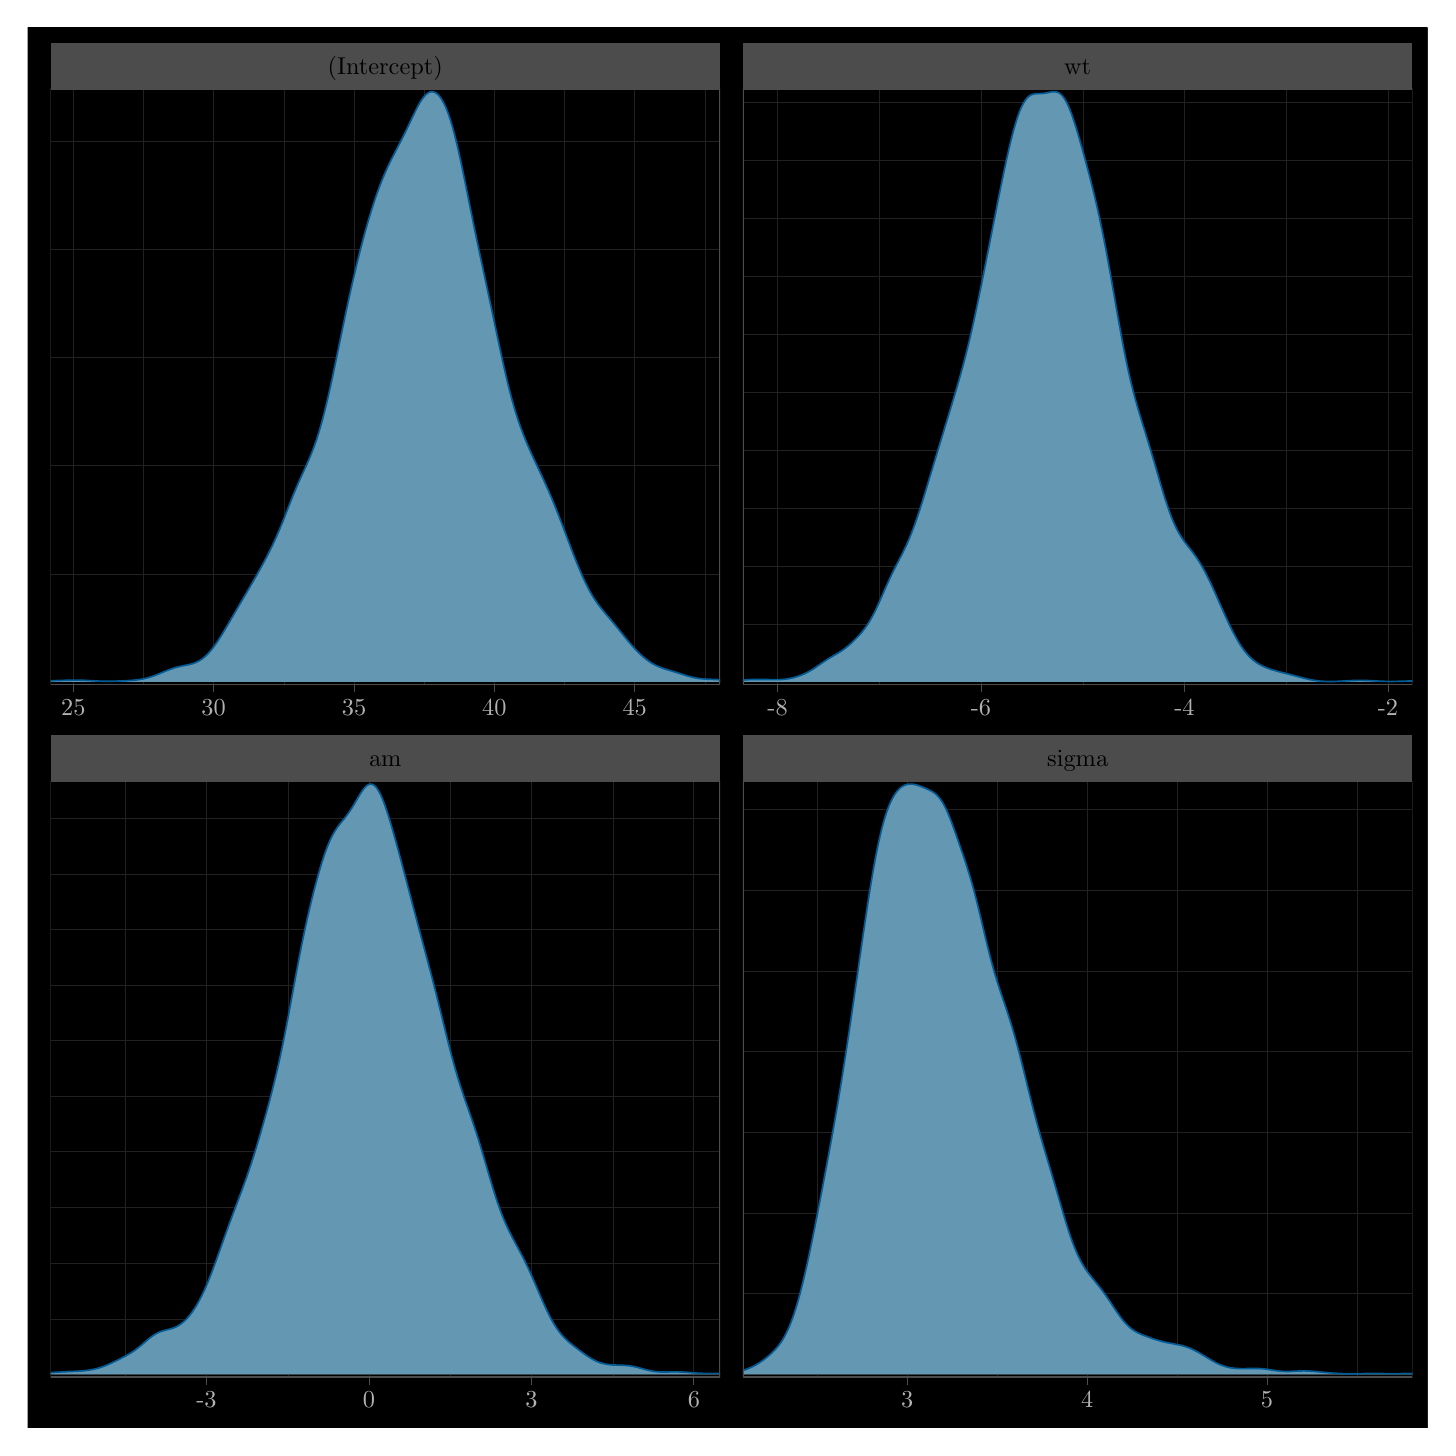
\begin{tikzpicture}[x=1pt,y=1pt]
\definecolor{fillColor}{RGB}{255,255,255}
\path[use as bounding box,fill=fillColor,fill opacity=0.00] (0,0) rectangle (505.89,505.89);
\begin{scope}
\path[clip] (  0.00,  0.00) rectangle (505.89,505.89);
\definecolor{drawColor}{RGB}{0,0,0}
\definecolor{fillColor}{RGB}{0,0,0}

\path[draw=drawColor,line width= 0.6pt,line join=round,line cap=round,fill=fillColor] (  0.00,  0.00) rectangle (505.89,505.89);
\end{scope}
\begin{scope}
\path[clip] (  8.25,268.42) rectangle (250.19,483.82);
\definecolor{fillColor}{RGB}{0,0,0}

\path[fill=fillColor] (  8.25,268.42) rectangle (250.19,483.82);
\definecolor{drawColor}{gray}{0.13}

\path[draw=drawColor,line width= 0.1pt,line join=round] (  8.25,308.57) --
	(250.19,308.57);

\path[draw=drawColor,line width= 0.1pt,line join=round] (  8.25,386.74) --
	(250.19,386.74);

\path[draw=drawColor,line width= 0.1pt,line join=round] (  8.25,464.91) --
	(250.19,464.91);

\path[draw=drawColor,line width= 0.1pt,line join=round] ( 41.86,268.42) --
	( 41.86,483.82);

\path[draw=drawColor,line width= 0.1pt,line join=round] ( 92.57,268.42) --
	( 92.57,483.82);

\path[draw=drawColor,line width= 0.1pt,line join=round] (143.28,268.42) --
	(143.28,483.82);

\path[draw=drawColor,line width= 0.1pt,line join=round] (193.99,268.42) --
	(193.99,483.82);

\path[draw=drawColor,line width= 0.1pt,line join=round] (244.71,268.42) --
	(244.71,483.82);

\path[draw=drawColor,line width= 0.3pt,line join=round] (  8.25,269.48) --
	(250.19,269.48);

\path[draw=drawColor,line width= 0.3pt,line join=round] (  8.25,347.65) --
	(250.19,347.65);

\path[draw=drawColor,line width= 0.3pt,line join=round] (  8.25,425.83) --
	(250.19,425.83);

\path[draw=drawColor,line width= 0.3pt,line join=round] ( 16.50,268.42) --
	( 16.50,483.82);

\path[draw=drawColor,line width= 0.3pt,line join=round] ( 67.21,268.42) --
	( 67.21,483.82);

\path[draw=drawColor,line width= 0.3pt,line join=round] (117.93,268.42) --
	(117.93,483.82);

\path[draw=drawColor,line width= 0.3pt,line join=round] (168.64,268.42) --
	(168.64,483.82);

\path[draw=drawColor,line width= 0.3pt,line join=round] (219.35,268.42) --
	(219.35,483.82);
\definecolor{fillColor}{RGB}{100,151,177}

\path[fill=fillColor] (  8.25,269.88) --
	(  8.72,269.90) --
	(  9.20,269.91) --
	(  9.67,269.93) --
	( 10.14,269.94) --
	( 10.62,269.96) --
	( 11.09,269.97) --
	( 11.56,269.99) --
	( 12.04,270.00) --
	( 12.51,270.02) --
	( 12.98,270.03) --
	( 13.46,270.05) --
	( 13.93,270.06) --
	( 14.41,270.08) --
	( 14.88,270.09) --
	( 15.35,270.10) --
	( 15.83,270.11) --
	( 16.30,270.12) --
	( 16.77,270.12) --
	( 17.25,270.13) --
	( 17.72,270.13) --
	( 18.19,270.12) --
	( 18.67,270.11) --
	( 19.14,270.10) --
	( 19.61,270.09) --
	( 20.09,270.07) --
	( 20.56,270.05) --
	( 21.03,270.03) --
	( 21.51,270.00) --
	( 21.98,269.98) --
	( 22.45,269.95) --
	( 22.93,269.92) --
	( 23.40,269.89) --
	( 23.87,269.87) --
	( 24.35,269.84) --
	( 24.82,269.81) --
	( 25.30,269.79) --
	( 25.77,269.77) --
	( 26.24,269.75) --
	( 26.72,269.74) --
	( 27.19,269.72) --
	( 27.66,269.72) --
	( 28.14,269.71) --
	( 28.61,269.71) --
	( 29.08,269.71) --
	( 29.56,269.71) --
	( 30.03,269.72) --
	( 30.50,269.73) --
	( 30.98,269.74) --
	( 31.45,269.75) --
	( 31.92,269.76) --
	( 32.40,269.78) --
	( 32.87,269.80) --
	( 33.34,269.81) --
	( 33.82,269.83) --
	( 34.29,269.85) --
	( 34.76,269.87) --
	( 35.24,269.90) --
	( 35.71,269.92) --
	( 36.18,269.94) --
	( 36.66,269.97) --
	( 37.13,270.00) --
	( 37.61,270.04) --
	( 38.08,270.07) --
	( 38.55,270.12) --
	( 39.03,270.16) --
	( 39.50,270.22) --
	( 39.97,270.28) --
	( 40.45,270.35) --
	( 40.92,270.42) --
	( 41.39,270.51) --
	( 41.87,270.60) --
	( 42.34,270.71) --
	( 42.81,270.82) --
	( 43.29,270.94) --
	( 43.76,271.08) --
	( 44.23,271.22) --
	( 44.71,271.37) --
	( 45.18,271.53) --
	( 45.65,271.70) --
	( 46.13,271.88) --
	( 46.60,272.06) --
	( 47.07,272.25) --
	( 47.55,272.44) --
	( 48.02,272.63) --
	( 48.50,272.83) --
	( 48.97,273.03) --
	( 49.44,273.22) --
	( 49.92,273.42) --
	( 50.39,273.61) --
	( 50.86,273.79) --
	( 51.34,273.97) --
	( 51.81,274.14) --
	( 52.28,274.31) --
	( 52.76,274.46) --
	( 53.23,274.61) --
	( 53.70,274.74) --
	( 54.18,274.87) --
	( 54.65,274.98) --
	( 55.12,275.09) --
	( 55.60,275.20) --
	( 56.07,275.29) --
	( 56.54,275.39) --
	( 57.02,275.48) --
	( 57.49,275.57) --
	( 57.96,275.67) --
	( 58.44,275.78) --
	( 58.91,275.89) --
	( 59.39,276.03) --
	( 59.86,276.17) --
	( 60.33,276.34) --
	( 60.81,276.53) --
	( 61.28,276.74) --
	( 61.75,276.98) --
	( 62.23,277.25) --
	( 62.70,277.56) --
	( 63.17,277.89) --
	( 63.65,278.27) --
	( 64.12,278.67) --
	( 64.59,279.11) --
	( 65.07,279.58) --
	( 65.54,280.09) --
	( 66.01,280.64) --
	( 66.49,281.22) --
	( 66.96,281.82) --
	( 67.43,282.46) --
	( 67.91,283.12) --
	( 68.38,283.80) --
	( 68.85,284.51) --
	( 69.33,285.24) --
	( 69.80,285.99) --
	( 70.28,286.75) --
	( 70.75,287.52) --
	( 71.22,288.30) --
	( 71.70,289.10) --
	( 72.17,289.90) --
	( 72.64,290.70) --
	( 73.12,291.51) --
	( 73.59,292.33) --
	( 74.06,293.14) --
	( 74.54,293.95) --
	( 75.01,294.77) --
	( 75.48,295.58) --
	( 75.96,296.39) --
	( 76.43,297.21) --
	( 76.90,298.01) --
	( 77.38,298.82) --
	( 77.85,299.63) --
	( 78.32,300.44) --
	( 78.80,301.25) --
	( 79.27,302.05) --
	( 79.74,302.86) --
	( 80.22,303.67) --
	( 80.69,304.49) --
	( 81.16,305.30) --
	( 81.64,306.13) --
	( 82.11,306.95) --
	( 82.59,307.78) --
	( 83.06,308.62) --
	( 83.53,309.46) --
	( 84.01,310.31) --
	( 84.48,311.16) --
	( 84.95,312.03) --
	( 85.43,312.90) --
	( 85.90,313.79) --
	( 86.37,314.69) --
	( 86.85,315.61) --
	( 87.32,316.54) --
	( 87.79,317.49) --
	( 88.27,318.46) --
	( 88.74,319.46) --
	( 89.21,320.48) --
	( 89.69,321.52) --
	( 90.16,322.59) --
	( 90.63,323.69) --
	( 91.11,324.82) --
	( 91.58,325.96) --
	( 92.05,327.13) --
	( 92.53,328.32) --
	( 93.00,329.52) --
	( 93.48,330.73) --
	( 93.95,331.94) --
	( 94.42,333.15) --
	( 94.90,334.35) --
	( 95.37,335.55) --
	( 95.84,336.72) --
	( 96.32,337.88) --
	( 96.79,339.02) --
	( 97.26,340.14) --
	( 97.74,341.22) --
	( 98.21,342.29) --
	( 98.68,343.35) --
	( 99.16,344.39) --
	( 99.63,345.42) --
	(100.10,346.45) --
	(100.58,347.48) --
	(101.05,348.54) --
	(101.52,349.61) --
	(102.00,350.72) --
	(102.47,351.87) --
	(102.94,353.06) --
	(103.42,354.31) --
	(103.89,355.62) --
	(104.37,357.01) --
	(104.84,358.47) --
	(105.31,360.00) --
	(105.79,361.61) --
	(106.26,363.29) --
	(106.73,365.04) --
	(107.21,366.89) --
	(107.68,368.80) --
	(108.15,370.77) --
	(108.63,372.81) --
	(109.10,374.90) --
	(109.57,377.04) --
	(110.05,379.23) --
	(110.52,381.46) --
	(110.99,383.71) --
	(111.47,385.99) --
	(111.94,388.28) --
	(112.41,390.58) --
	(112.89,392.88) --
	(113.36,395.18) --
	(113.83,397.47) --
	(114.31,399.74) --
	(114.78,402.00) --
	(115.26,404.23) --
	(115.73,406.44) --
	(116.20,408.62) --
	(116.68,410.77) --
	(117.15,412.88) --
	(117.62,414.95) --
	(118.10,416.99) --
	(118.57,419.00) --
	(119.04,420.96) --
	(119.52,422.89) --
	(119.99,424.78) --
	(120.46,426.62) --
	(120.94,428.43) --
	(121.41,430.19) --
	(121.88,431.93) --
	(122.36,433.62) --
	(122.83,435.27) --
	(123.30,436.88) --
	(123.78,438.45) --
	(124.25,439.99) --
	(124.72,441.48) --
	(125.20,442.94) --
	(125.67,444.35) --
	(126.14,445.73) --
	(126.62,447.05) --
	(127.09,448.34) --
	(127.57,449.58) --
	(128.04,450.79) --
	(128.51,451.95) --
	(128.99,453.08) --
	(129.46,454.16) --
	(129.93,455.21) --
	(130.41,456.22) --
	(130.88,457.21) --
	(131.35,458.17) --
	(131.83,459.11) --
	(132.30,460.03) --
	(132.77,460.94) --
	(133.25,461.85) --
	(133.72,462.75) --
	(134.19,463.66) --
	(134.67,464.57) --
	(135.14,465.49) --
	(135.61,466.43) --
	(136.09,467.38) --
	(136.56,468.35) --
	(137.03,469.33) --
	(137.51,470.32) --
	(137.98,471.32) --
	(138.46,472.33) --
	(138.93,473.33) --
	(139.40,474.33) --
	(139.88,475.30) --
	(140.35,476.25) --
	(140.82,477.17) --
	(141.30,478.05) --
	(141.77,478.87) --
	(142.24,479.64) --
	(142.72,480.32) --
	(143.19,480.93) --
	(143.66,481.46) --
	(144.14,481.91) --
	(144.61,482.27) --
	(145.08,482.53) --
	(145.56,482.70) --
	(146.03,482.75) --
	(146.50,482.71) --
	(146.98,482.58) --
	(147.45,482.34) --
	(147.92,482.01) --
	(148.40,481.58) --
	(148.87,481.03) --
	(149.35,480.38) --
	(149.82,479.62) --
	(150.29,478.76) --
	(150.77,477.80) --
	(151.24,476.73) --
	(151.71,475.55) --
	(152.19,474.24) --
	(152.66,472.81) --
	(153.13,471.28) --
	(153.61,469.65) --
	(154.08,467.91) --
	(154.55,466.07) --
	(155.03,464.14) --
	(155.50,462.11) --
	(155.97,460.00) --
	(156.45,457.83) --
	(156.92,455.60) --
	(157.39,453.32) --
	(157.87,451.01) --
	(158.34,448.67) --
	(158.81,446.31) --
	(159.29,443.95) --
	(159.76,441.59) --
	(160.24,439.24) --
	(160.71,436.90) --
	(161.18,434.58) --
	(161.66,432.28) --
	(162.13,430.00) --
	(162.60,427.74) --
	(163.08,425.50) --
	(163.55,423.27) --
	(164.02,421.06) --
	(164.50,418.85) --
	(164.97,416.65) --
	(165.44,414.44) --
	(165.92,412.24) --
	(166.39,410.02) --
	(166.86,407.80) --
	(167.34,405.58) --
	(167.81,403.34) --
	(168.28,401.09) --
	(168.76,398.85) --
	(169.23,396.60) --
	(169.70,394.36) --
	(170.18,392.12) --
	(170.65,389.91) --
	(171.12,387.71) --
	(171.60,385.55) --
	(172.07,383.43) --
	(172.55,381.35) --
	(173.02,379.32) --
	(173.49,377.35) --
	(173.97,375.43) --
	(174.44,373.59) --
	(174.91,371.81) --
	(175.39,370.11) --
	(175.86,368.46) --
	(176.33,366.89) --
	(176.81,365.38) --
	(177.28,363.93) --
	(177.75,362.55) --
	(178.23,361.22) --
	(178.70,359.94) --
	(179.17,358.71) --
	(179.65,357.52) --
	(180.12,356.36) --
	(180.59,355.23) --
	(181.07,354.14) --
	(181.54,353.06) --
	(182.01,352.01) --
	(182.49,350.97) --
	(182.96,349.94) --
	(183.44,348.92) --
	(183.91,347.91) --
	(184.38,346.90) --
	(184.86,345.89) --
	(185.33,344.88) --
	(185.80,343.86) --
	(186.28,342.84) --
	(186.75,341.81) --
	(187.22,340.76) --
	(187.70,339.70) --
	(188.17,338.63) --
	(188.64,337.53) --
	(189.12,336.42) --
	(189.59,335.30) --
	(190.06,334.15) --
	(190.54,332.98) --
	(191.01,331.79) --
	(191.48,330.59) --
	(191.96,329.38) --
	(192.43,328.15) --
	(192.90,326.91) --
	(193.38,325.66) --
	(193.85,324.41) --
	(194.33,323.16) --
	(194.80,321.90) --
	(195.27,320.65) --
	(195.75,319.40) --
	(196.22,318.15) --
	(196.69,316.92) --
	(197.17,315.69) --
	(197.64,314.49) --
	(198.11,313.29) --
	(198.59,312.12) --
	(199.06,310.96) --
	(199.53,309.83) --
	(200.01,308.73) --
	(200.48,307.65) --
	(200.95,306.61) --
	(201.43,305.60) --
	(201.90,304.62) --
	(202.37,303.68) --
	(202.85,302.77) --
	(203.32,301.90) --
	(203.79,301.08) --
	(204.27,300.29) --
	(204.74,299.54) --
	(205.22,298.82) --
	(205.69,298.13) --
	(206.16,297.47) --
	(206.64,296.84) --
	(207.11,296.23) --
	(207.58,295.64) --
	(208.06,295.06) --
	(208.53,294.49) --
	(209.00,293.93) --
	(209.48,293.38) --
	(209.95,292.82) --
	(210.42,292.27) --
	(210.90,291.71) --
	(211.37,291.14) --
	(211.84,290.57) --
	(212.32,290.00) --
	(212.79,289.42) --
	(213.26,288.83) --
	(213.74,288.24) --
	(214.21,287.65) --
	(214.68,287.06) --
	(215.16,286.47) --
	(215.63,285.88) --
	(216.10,285.29) --
	(216.58,284.72) --
	(217.05,284.15) --
	(217.53,283.58) --
	(218.00,283.03) --
	(218.47,282.49) --
	(218.95,281.96) --
	(219.42,281.45) --
	(219.89,280.94) --
	(220.37,280.46) --
	(220.84,279.99) --
	(221.31,279.53) --
	(221.79,279.09) --
	(222.26,278.67) --
	(222.73,278.26) --
	(223.21,277.87) --
	(223.68,277.51) --
	(224.15,277.16) --
	(224.63,276.82) --
	(225.10,276.51) --
	(225.57,276.22) --
	(226.05,275.94) --
	(226.52,275.69) --
	(226.99,275.45) --
	(227.47,275.22) --
	(227.94,275.01) --
	(228.42,274.82) --
	(228.89,274.64) --
	(229.36,274.47) --
	(229.84,274.30) --
	(230.31,274.15) --
	(230.78,274.00) --
	(231.26,273.85) --
	(231.73,273.71) --
	(232.20,273.57) --
	(232.68,273.43) --
	(233.15,273.29) --
	(233.62,273.14) --
	(234.10,273.00) --
	(234.57,272.85) --
	(235.04,272.70) --
	(235.52,272.54) --
	(235.99,272.39) --
	(236.46,272.24) --
	(236.94,272.08) --
	(237.41,271.93) --
	(237.88,271.79) --
	(238.36,271.64) --
	(238.83,271.51) --
	(239.31,271.38) --
	(239.78,271.26) --
	(240.25,271.14) --
	(240.73,271.04) --
	(241.20,270.94) --
	(241.67,270.86) --
	(242.15,270.78) --
	(242.62,270.72) --
	(243.09,270.66) --
	(243.57,270.61) --
	(244.04,270.57) --
	(244.51,270.53) --
	(244.99,270.50) --
	(245.46,270.47) --
	(245.93,270.45) --
	(246.41,270.43) --
	(246.88,270.41) --
	(247.35,270.39) --
	(247.83,270.37) --
	(248.30,270.35) --
	(248.77,270.33) --
	(249.25,270.31) --
	(249.72,270.28) --
	(250.19,270.25) --
	(250.19,269.48) --
	(249.72,269.48) --
	(249.25,269.48) --
	(248.77,269.48) --
	(248.30,269.48) --
	(247.83,269.48) --
	(247.35,269.48) --
	(246.88,269.48) --
	(246.41,269.48) --
	(245.93,269.48) --
	(245.46,269.48) --
	(244.99,269.48) --
	(244.51,269.48) --
	(244.04,269.48) --
	(243.57,269.48) --
	(243.09,269.48) --
	(242.62,269.48) --
	(242.15,269.48) --
	(241.67,269.48) --
	(241.20,269.48) --
	(240.73,269.48) --
	(240.25,269.48) --
	(239.78,269.48) --
	(239.31,269.48) --
	(238.83,269.48) --
	(238.36,269.48) --
	(237.88,269.48) --
	(237.41,269.48) --
	(236.94,269.48) --
	(236.46,269.48) --
	(235.99,269.48) --
	(235.52,269.48) --
	(235.04,269.48) --
	(234.57,269.48) --
	(234.10,269.48) --
	(233.62,269.48) --
	(233.15,269.48) --
	(232.68,269.48) --
	(232.20,269.48) --
	(231.73,269.48) --
	(231.26,269.48) --
	(230.78,269.48) --
	(230.31,269.48) --
	(229.84,269.48) --
	(229.36,269.48) --
	(228.89,269.48) --
	(228.42,269.48) --
	(227.94,269.48) --
	(227.47,269.48) --
	(226.99,269.48) --
	(226.52,269.48) --
	(226.05,269.48) --
	(225.57,269.48) --
	(225.10,269.48) --
	(224.63,269.48) --
	(224.15,269.48) --
	(223.68,269.48) --
	(223.21,269.48) --
	(222.73,269.48) --
	(222.26,269.48) --
	(221.79,269.48) --
	(221.31,269.48) --
	(220.84,269.48) --
	(220.37,269.48) --
	(219.89,269.48) --
	(219.42,269.48) --
	(218.95,269.48) --
	(218.47,269.48) --
	(218.00,269.48) --
	(217.53,269.48) --
	(217.05,269.48) --
	(216.58,269.48) --
	(216.10,269.48) --
	(215.63,269.48) --
	(215.16,269.48) --
	(214.68,269.48) --
	(214.21,269.48) --
	(213.74,269.48) --
	(213.26,269.48) --
	(212.79,269.48) --
	(212.32,269.48) --
	(211.84,269.48) --
	(211.37,269.48) --
	(210.90,269.48) --
	(210.42,269.48) --
	(209.95,269.48) --
	(209.48,269.48) --
	(209.00,269.48) --
	(208.53,269.48) --
	(208.06,269.48) --
	(207.58,269.48) --
	(207.11,269.48) --
	(206.64,269.48) --
	(206.16,269.48) --
	(205.69,269.48) --
	(205.22,269.48) --
	(204.74,269.48) --
	(204.27,269.48) --
	(203.79,269.48) --
	(203.32,269.48) --
	(202.85,269.48) --
	(202.37,269.48) --
	(201.90,269.48) --
	(201.43,269.48) --
	(200.95,269.48) --
	(200.48,269.48) --
	(200.01,269.48) --
	(199.53,269.48) --
	(199.06,269.48) --
	(198.59,269.48) --
	(198.11,269.48) --
	(197.64,269.48) --
	(197.17,269.48) --
	(196.69,269.48) --
	(196.22,269.48) --
	(195.75,269.48) --
	(195.27,269.48) --
	(194.80,269.48) --
	(194.33,269.48) --
	(193.85,269.48) --
	(193.38,269.48) --
	(192.90,269.48) --
	(192.43,269.48) --
	(191.96,269.48) --
	(191.48,269.48) --
	(191.01,269.48) --
	(190.54,269.48) --
	(190.06,269.48) --
	(189.59,269.48) --
	(189.12,269.48) --
	(188.64,269.48) --
	(188.17,269.48) --
	(187.70,269.48) --
	(187.22,269.48) --
	(186.75,269.48) --
	(186.28,269.48) --
	(185.80,269.48) --
	(185.33,269.48) --
	(184.86,269.48) --
	(184.38,269.48) --
	(183.91,269.48) --
	(183.44,269.48) --
	(182.96,269.48) --
	(182.49,269.48) --
	(182.01,269.48) --
	(181.54,269.48) --
	(181.07,269.48) --
	(180.59,269.48) --
	(180.12,269.48) --
	(179.65,269.48) --
	(179.17,269.48) --
	(178.70,269.48) --
	(178.23,269.48) --
	(177.75,269.48) --
	(177.28,269.48) --
	(176.81,269.48) --
	(176.33,269.48) --
	(175.86,269.48) --
	(175.39,269.48) --
	(174.91,269.48) --
	(174.44,269.48) --
	(173.97,269.48) --
	(173.49,269.48) --
	(173.02,269.48) --
	(172.55,269.48) --
	(172.07,269.48) --
	(171.60,269.48) --
	(171.12,269.48) --
	(170.65,269.48) --
	(170.18,269.48) --
	(169.70,269.48) --
	(169.23,269.48) --
	(168.76,269.48) --
	(168.28,269.48) --
	(167.81,269.48) --
	(167.34,269.48) --
	(166.86,269.48) --
	(166.39,269.48) --
	(165.92,269.48) --
	(165.44,269.48) --
	(164.97,269.48) --
	(164.50,269.48) --
	(164.02,269.48) --
	(163.55,269.48) --
	(163.08,269.48) --
	(162.60,269.48) --
	(162.13,269.48) --
	(161.66,269.48) --
	(161.18,269.48) --
	(160.71,269.48) --
	(160.24,269.48) --
	(159.76,269.48) --
	(159.29,269.48) --
	(158.81,269.48) --
	(158.34,269.48) --
	(157.87,269.48) --
	(157.39,269.48) --
	(156.92,269.48) --
	(156.45,269.48) --
	(155.97,269.48) --
	(155.50,269.48) --
	(155.03,269.48) --
	(154.55,269.48) --
	(154.08,269.48) --
	(153.61,269.48) --
	(153.13,269.48) --
	(152.66,269.48) --
	(152.19,269.48) --
	(151.71,269.48) --
	(151.24,269.48) --
	(150.77,269.48) --
	(150.29,269.48) --
	(149.82,269.48) --
	(149.35,269.48) --
	(148.87,269.48) --
	(148.40,269.48) --
	(147.92,269.48) --
	(147.45,269.48) --
	(146.98,269.48) --
	(146.50,269.48) --
	(146.03,269.48) --
	(145.56,269.48) --
	(145.08,269.48) --
	(144.61,269.48) --
	(144.14,269.48) --
	(143.66,269.48) --
	(143.19,269.48) --
	(142.72,269.48) --
	(142.24,269.48) --
	(141.77,269.48) --
	(141.30,269.48) --
	(140.82,269.48) --
	(140.35,269.48) --
	(139.88,269.48) --
	(139.40,269.48) --
	(138.93,269.48) --
	(138.46,269.48) --
	(137.98,269.48) --
	(137.51,269.48) --
	(137.03,269.48) --
	(136.56,269.48) --
	(136.09,269.48) --
	(135.61,269.48) --
	(135.14,269.48) --
	(134.67,269.48) --
	(134.19,269.48) --
	(133.72,269.48) --
	(133.25,269.48) --
	(132.77,269.48) --
	(132.30,269.48) --
	(131.83,269.48) --
	(131.35,269.48) --
	(130.88,269.48) --
	(130.41,269.48) --
	(129.93,269.48) --
	(129.46,269.48) --
	(128.99,269.48) --
	(128.51,269.48) --
	(128.04,269.48) --
	(127.57,269.48) --
	(127.09,269.48) --
	(126.62,269.48) --
	(126.14,269.48) --
	(125.67,269.48) --
	(125.20,269.48) --
	(124.72,269.48) --
	(124.25,269.48) --
	(123.78,269.48) --
	(123.30,269.48) --
	(122.83,269.48) --
	(122.36,269.48) --
	(121.88,269.48) --
	(121.41,269.48) --
	(120.94,269.48) --
	(120.46,269.48) --
	(119.99,269.48) --
	(119.52,269.48) --
	(119.04,269.48) --
	(118.57,269.48) --
	(118.10,269.48) --
	(117.62,269.48) --
	(117.15,269.48) --
	(116.68,269.48) --
	(116.20,269.48) --
	(115.73,269.48) --
	(115.26,269.48) --
	(114.78,269.48) --
	(114.31,269.48) --
	(113.83,269.48) --
	(113.36,269.48) --
	(112.89,269.48) --
	(112.41,269.48) --
	(111.94,269.48) --
	(111.47,269.48) --
	(110.99,269.48) --
	(110.52,269.48) --
	(110.05,269.48) --
	(109.57,269.48) --
	(109.10,269.48) --
	(108.63,269.48) --
	(108.15,269.48) --
	(107.68,269.48) --
	(107.21,269.48) --
	(106.73,269.48) --
	(106.26,269.48) --
	(105.79,269.48) --
	(105.31,269.48) --
	(104.84,269.48) --
	(104.37,269.48) --
	(103.89,269.48) --
	(103.42,269.48) --
	(102.94,269.48) --
	(102.47,269.48) --
	(102.00,269.48) --
	(101.52,269.48) --
	(101.05,269.48) --
	(100.58,269.48) --
	(100.10,269.48) --
	( 99.63,269.48) --
	( 99.16,269.48) --
	( 98.68,269.48) --
	( 98.21,269.48) --
	( 97.74,269.48) --
	( 97.26,269.48) --
	( 96.79,269.48) --
	( 96.32,269.48) --
	( 95.84,269.48) --
	( 95.37,269.48) --
	( 94.90,269.48) --
	( 94.42,269.48) --
	( 93.95,269.48) --
	( 93.48,269.48) --
	( 93.00,269.48) --
	( 92.53,269.48) --
	( 92.05,269.48) --
	( 91.58,269.48) --
	( 91.11,269.48) --
	( 90.63,269.48) --
	( 90.16,269.48) --
	( 89.69,269.48) --
	( 89.21,269.48) --
	( 88.74,269.48) --
	( 88.27,269.48) --
	( 87.79,269.48) --
	( 87.32,269.48) --
	( 86.85,269.48) --
	( 86.37,269.48) --
	( 85.90,269.48) --
	( 85.43,269.48) --
	( 84.95,269.48) --
	( 84.48,269.48) --
	( 84.01,269.48) --
	( 83.53,269.48) --
	( 83.06,269.48) --
	( 82.59,269.48) --
	( 82.11,269.48) --
	( 81.64,269.48) --
	( 81.16,269.48) --
	( 80.69,269.48) --
	( 80.22,269.48) --
	( 79.74,269.48) --
	( 79.27,269.48) --
	( 78.80,269.48) --
	( 78.32,269.48) --
	( 77.85,269.48) --
	( 77.38,269.48) --
	( 76.90,269.48) --
	( 76.43,269.48) --
	( 75.96,269.48) --
	( 75.48,269.48) --
	( 75.01,269.48) --
	( 74.54,269.48) --
	( 74.06,269.48) --
	( 73.59,269.48) --
	( 73.12,269.48) --
	( 72.64,269.48) --
	( 72.17,269.48) --
	( 71.70,269.48) --
	( 71.22,269.48) --
	( 70.75,269.48) --
	( 70.28,269.48) --
	( 69.80,269.48) --
	( 69.33,269.48) --
	( 68.85,269.48) --
	( 68.38,269.48) --
	( 67.91,269.48) --
	( 67.43,269.48) --
	( 66.96,269.48) --
	( 66.49,269.48) --
	( 66.01,269.48) --
	( 65.54,269.48) --
	( 65.07,269.48) --
	( 64.59,269.48) --
	( 64.12,269.48) --
	( 63.65,269.48) --
	( 63.17,269.48) --
	( 62.70,269.48) --
	( 62.23,269.48) --
	( 61.75,269.48) --
	( 61.28,269.48) --
	( 60.81,269.48) --
	( 60.33,269.48) --
	( 59.86,269.48) --
	( 59.39,269.48) --
	( 58.91,269.48) --
	( 58.44,269.48) --
	( 57.96,269.48) --
	( 57.49,269.48) --
	( 57.02,269.48) --
	( 56.54,269.48) --
	( 56.07,269.48) --
	( 55.60,269.48) --
	( 55.12,269.48) --
	( 54.65,269.48) --
	( 54.18,269.48) --
	( 53.70,269.48) --
	( 53.23,269.48) --
	( 52.76,269.48) --
	( 52.28,269.48) --
	( 51.81,269.48) --
	( 51.34,269.48) --
	( 50.86,269.48) --
	( 50.39,269.48) --
	( 49.92,269.48) --
	( 49.44,269.48) --
	( 48.97,269.48) --
	( 48.50,269.48) --
	( 48.02,269.48) --
	( 47.55,269.48) --
	( 47.07,269.48) --
	( 46.60,269.48) --
	( 46.13,269.48) --
	( 45.65,269.48) --
	( 45.18,269.48) --
	( 44.71,269.48) --
	( 44.23,269.48) --
	( 43.76,269.48) --
	( 43.29,269.48) --
	( 42.81,269.48) --
	( 42.34,269.48) --
	( 41.87,269.48) --
	( 41.39,269.48) --
	( 40.92,269.48) --
	( 40.45,269.48) --
	( 39.97,269.48) --
	( 39.50,269.48) --
	( 39.03,269.48) --
	( 38.55,269.48) --
	( 38.08,269.48) --
	( 37.61,269.48) --
	( 37.13,269.48) --
	( 36.66,269.48) --
	( 36.18,269.48) --
	( 35.71,269.48) --
	( 35.24,269.48) --
	( 34.76,269.48) --
	( 34.29,269.48) --
	( 33.82,269.48) --
	( 33.34,269.48) --
	( 32.87,269.48) --
	( 32.40,269.48) --
	( 31.92,269.48) --
	( 31.45,269.48) --
	( 30.98,269.48) --
	( 30.50,269.48) --
	( 30.03,269.48) --
	( 29.56,269.48) --
	( 29.08,269.48) --
	( 28.61,269.48) --
	( 28.14,269.48) --
	( 27.66,269.48) --
	( 27.19,269.48) --
	( 26.72,269.48) --
	( 26.24,269.48) --
	( 25.77,269.48) --
	( 25.30,269.48) --
	( 24.82,269.48) --
	( 24.35,269.48) --
	( 23.87,269.48) --
	( 23.40,269.48) --
	( 22.93,269.48) --
	( 22.45,269.48) --
	( 21.98,269.48) --
	( 21.51,269.48) --
	( 21.03,269.48) --
	( 20.56,269.48) --
	( 20.09,269.48) --
	( 19.61,269.48) --
	( 19.14,269.48) --
	( 18.67,269.48) --
	( 18.19,269.48) --
	( 17.72,269.48) --
	( 17.25,269.48) --
	( 16.77,269.48) --
	( 16.30,269.48) --
	( 15.83,269.48) --
	( 15.35,269.48) --
	( 14.88,269.48) --
	( 14.41,269.48) --
	( 13.93,269.48) --
	( 13.46,269.48) --
	( 12.98,269.48) --
	( 12.51,269.48) --
	( 12.04,269.48) --
	( 11.56,269.48) --
	( 11.09,269.48) --
	( 10.62,269.48) --
	( 10.14,269.48) --
	(  9.67,269.48) --
	(  9.20,269.48) --
	(  8.72,269.48) --
	(  8.25,269.48) --
	cycle;
\definecolor{drawColor}{RGB}{0,91,150}

\path[draw=drawColor,line width= 0.6pt,line join=round,line cap=round] (  8.25,269.88) --
	(  8.72,269.90) --
	(  9.20,269.91) --
	(  9.67,269.93) --
	( 10.14,269.94) --
	( 10.62,269.96) --
	( 11.09,269.97) --
	( 11.56,269.99) --
	( 12.04,270.00) --
	( 12.51,270.02) --
	( 12.98,270.03) --
	( 13.46,270.05) --
	( 13.93,270.06) --
	( 14.41,270.08) --
	( 14.88,270.09) --
	( 15.35,270.10) --
	( 15.83,270.11) --
	( 16.30,270.12) --
	( 16.77,270.12) --
	( 17.25,270.13) --
	( 17.72,270.13) --
	( 18.19,270.12) --
	( 18.67,270.11) --
	( 19.14,270.10) --
	( 19.61,270.09) --
	( 20.09,270.07) --
	( 20.56,270.05) --
	( 21.03,270.03) --
	( 21.51,270.00) --
	( 21.98,269.98) --
	( 22.45,269.95) --
	( 22.93,269.92) --
	( 23.40,269.89) --
	( 23.87,269.87) --
	( 24.35,269.84) --
	( 24.82,269.81) --
	( 25.30,269.79) --
	( 25.77,269.77) --
	( 26.24,269.75) --
	( 26.72,269.74) --
	( 27.19,269.72) --
	( 27.66,269.72) --
	( 28.14,269.71) --
	( 28.61,269.71) --
	( 29.08,269.71) --
	( 29.56,269.71) --
	( 30.03,269.72) --
	( 30.50,269.73) --
	( 30.98,269.74) --
	( 31.45,269.75) --
	( 31.92,269.76) --
	( 32.40,269.78) --
	( 32.87,269.80) --
	( 33.34,269.81) --
	( 33.82,269.83) --
	( 34.29,269.85) --
	( 34.76,269.87) --
	( 35.24,269.90) --
	( 35.71,269.92) --
	( 36.18,269.94) --
	( 36.66,269.97) --
	( 37.13,270.00) --
	( 37.61,270.04) --
	( 38.08,270.07) --
	( 38.55,270.12) --
	( 39.03,270.16) --
	( 39.50,270.22) --
	( 39.97,270.28) --
	( 40.45,270.35) --
	( 40.92,270.42) --
	( 41.39,270.51) --
	( 41.87,270.60) --
	( 42.34,270.71) --
	( 42.81,270.82) --
	( 43.29,270.94) --
	( 43.76,271.08) --
	( 44.23,271.22) --
	( 44.71,271.37) --
	( 45.18,271.53) --
	( 45.65,271.70) --
	( 46.13,271.88) --
	( 46.60,272.06) --
	( 47.07,272.25) --
	( 47.55,272.44) --
	( 48.02,272.63) --
	( 48.50,272.83) --
	( 48.97,273.03) --
	( 49.44,273.22) --
	( 49.92,273.42) --
	( 50.39,273.61) --
	( 50.86,273.79) --
	( 51.34,273.97) --
	( 51.81,274.14) --
	( 52.28,274.31) --
	( 52.76,274.46) --
	( 53.23,274.61) --
	( 53.70,274.74) --
	( 54.18,274.87) --
	( 54.65,274.98) --
	( 55.12,275.09) --
	( 55.60,275.20) --
	( 56.07,275.29) --
	( 56.54,275.39) --
	( 57.02,275.48) --
	( 57.49,275.57) --
	( 57.96,275.67) --
	( 58.44,275.78) --
	( 58.91,275.89) --
	( 59.39,276.03) --
	( 59.86,276.17) --
	( 60.33,276.34) --
	( 60.81,276.53) --
	( 61.28,276.74) --
	( 61.75,276.98) --
	( 62.23,277.25) --
	( 62.70,277.56) --
	( 63.17,277.89) --
	( 63.65,278.27) --
	( 64.12,278.67) --
	( 64.59,279.11) --
	( 65.07,279.58) --
	( 65.54,280.09) --
	( 66.01,280.64) --
	( 66.49,281.22) --
	( 66.96,281.82) --
	( 67.43,282.46) --
	( 67.91,283.12) --
	( 68.38,283.80) --
	( 68.85,284.51) --
	( 69.33,285.24) --
	( 69.80,285.99) --
	( 70.28,286.75) --
	( 70.75,287.52) --
	( 71.22,288.30) --
	( 71.70,289.10) --
	( 72.17,289.90) --
	( 72.64,290.70) --
	( 73.12,291.51) --
	( 73.59,292.33) --
	( 74.06,293.14) --
	( 74.54,293.95) --
	( 75.01,294.77) --
	( 75.48,295.58) --
	( 75.96,296.39) --
	( 76.43,297.21) --
	( 76.90,298.01) --
	( 77.38,298.82) --
	( 77.85,299.63) --
	( 78.32,300.44) --
	( 78.80,301.25) --
	( 79.27,302.05) --
	( 79.74,302.86) --
	( 80.22,303.67) --
	( 80.69,304.49) --
	( 81.16,305.30) --
	( 81.64,306.13) --
	( 82.11,306.95) --
	( 82.59,307.78) --
	( 83.06,308.62) --
	( 83.53,309.46) --
	( 84.01,310.31) --
	( 84.48,311.16) --
	( 84.95,312.03) --
	( 85.43,312.90) --
	( 85.90,313.79) --
	( 86.37,314.69) --
	( 86.85,315.61) --
	( 87.32,316.54) --
	( 87.79,317.49) --
	( 88.27,318.46) --
	( 88.74,319.46) --
	( 89.21,320.48) --
	( 89.69,321.52) --
	( 90.16,322.59) --
	( 90.63,323.69) --
	( 91.11,324.82) --
	( 91.58,325.96) --
	( 92.05,327.13) --
	( 92.53,328.32) --
	( 93.00,329.52) --
	( 93.48,330.73) --
	( 93.95,331.94) --
	( 94.42,333.15) --
	( 94.90,334.35) --
	( 95.37,335.55) --
	( 95.84,336.72) --
	( 96.32,337.88) --
	( 96.79,339.02) --
	( 97.26,340.14) --
	( 97.74,341.22) --
	( 98.21,342.29) --
	( 98.68,343.35) --
	( 99.16,344.39) --
	( 99.63,345.42) --
	(100.10,346.45) --
	(100.58,347.48) --
	(101.05,348.54) --
	(101.52,349.61) --
	(102.00,350.72) --
	(102.47,351.87) --
	(102.94,353.06) --
	(103.42,354.31) --
	(103.89,355.62) --
	(104.37,357.01) --
	(104.84,358.47) --
	(105.31,360.00) --
	(105.79,361.61) --
	(106.26,363.29) --
	(106.73,365.04) --
	(107.21,366.89) --
	(107.68,368.80) --
	(108.15,370.77) --
	(108.63,372.81) --
	(109.10,374.90) --
	(109.57,377.04) --
	(110.05,379.23) --
	(110.52,381.46) --
	(110.99,383.71) --
	(111.47,385.99) --
	(111.94,388.28) --
	(112.41,390.58) --
	(112.89,392.88) --
	(113.36,395.18) --
	(113.83,397.47) --
	(114.31,399.74) --
	(114.78,402.00) --
	(115.26,404.23) --
	(115.73,406.44) --
	(116.20,408.62) --
	(116.68,410.77) --
	(117.15,412.88) --
	(117.62,414.95) --
	(118.10,416.99) --
	(118.57,419.00) --
	(119.04,420.96) --
	(119.52,422.89) --
	(119.99,424.78) --
	(120.46,426.62) --
	(120.94,428.43) --
	(121.41,430.19) --
	(121.88,431.93) --
	(122.36,433.62) --
	(122.83,435.27) --
	(123.30,436.88) --
	(123.78,438.45) --
	(124.25,439.99) --
	(124.72,441.48) --
	(125.20,442.94) --
	(125.67,444.35) --
	(126.14,445.73) --
	(126.62,447.05) --
	(127.09,448.34) --
	(127.57,449.58) --
	(128.04,450.79) --
	(128.51,451.95) --
	(128.99,453.08) --
	(129.46,454.16) --
	(129.93,455.21) --
	(130.41,456.22) --
	(130.88,457.21) --
	(131.35,458.17) --
	(131.83,459.11) --
	(132.30,460.03) --
	(132.77,460.94) --
	(133.25,461.85) --
	(133.72,462.75) --
	(134.19,463.66) --
	(134.67,464.57) --
	(135.14,465.49) --
	(135.61,466.43) --
	(136.09,467.38) --
	(136.56,468.35) --
	(137.03,469.33) --
	(137.51,470.32) --
	(137.98,471.32) --
	(138.46,472.33) --
	(138.93,473.33) --
	(139.40,474.33) --
	(139.88,475.30) --
	(140.35,476.25) --
	(140.82,477.17) --
	(141.30,478.05) --
	(141.77,478.87) --
	(142.24,479.64) --
	(142.72,480.32) --
	(143.19,480.93) --
	(143.66,481.46) --
	(144.14,481.91) --
	(144.61,482.27) --
	(145.08,482.53) --
	(145.56,482.70) --
	(146.03,482.75) --
	(146.50,482.71) --
	(146.98,482.58) --
	(147.45,482.34) --
	(147.92,482.01) --
	(148.40,481.58) --
	(148.87,481.03) --
	(149.35,480.38) --
	(149.82,479.62) --
	(150.29,478.76) --
	(150.77,477.80) --
	(151.24,476.73) --
	(151.71,475.55) --
	(152.19,474.24) --
	(152.66,472.81) --
	(153.13,471.28) --
	(153.61,469.65) --
	(154.08,467.91) --
	(154.55,466.07) --
	(155.03,464.14) --
	(155.50,462.11) --
	(155.97,460.00) --
	(156.45,457.83) --
	(156.92,455.60) --
	(157.39,453.32) --
	(157.87,451.01) --
	(158.34,448.67) --
	(158.81,446.31) --
	(159.29,443.95) --
	(159.76,441.59) --
	(160.24,439.24) --
	(160.71,436.90) --
	(161.18,434.58) --
	(161.66,432.28) --
	(162.13,430.00) --
	(162.60,427.74) --
	(163.08,425.50) --
	(163.55,423.27) --
	(164.02,421.06) --
	(164.50,418.85) --
	(164.97,416.65) --
	(165.44,414.44) --
	(165.92,412.24) --
	(166.39,410.02) --
	(166.86,407.80) --
	(167.34,405.58) --
	(167.81,403.34) --
	(168.28,401.09) --
	(168.76,398.85) --
	(169.23,396.60) --
	(169.70,394.36) --
	(170.18,392.12) --
	(170.65,389.91) --
	(171.12,387.71) --
	(171.60,385.55) --
	(172.07,383.43) --
	(172.55,381.35) --
	(173.02,379.32) --
	(173.49,377.35) --
	(173.97,375.43) --
	(174.44,373.59) --
	(174.91,371.81) --
	(175.39,370.11) --
	(175.86,368.46) --
	(176.33,366.89) --
	(176.81,365.38) --
	(177.28,363.93) --
	(177.75,362.55) --
	(178.23,361.22) --
	(178.70,359.94) --
	(179.17,358.71) --
	(179.65,357.52) --
	(180.12,356.36) --
	(180.59,355.23) --
	(181.07,354.14) --
	(181.54,353.06) --
	(182.01,352.01) --
	(182.49,350.97) --
	(182.96,349.94) --
	(183.44,348.92) --
	(183.91,347.91) --
	(184.38,346.90) --
	(184.86,345.89) --
	(185.33,344.88) --
	(185.80,343.86) --
	(186.28,342.84) --
	(186.75,341.81) --
	(187.22,340.76) --
	(187.70,339.70) --
	(188.17,338.63) --
	(188.64,337.53) --
	(189.12,336.42) --
	(189.59,335.30) --
	(190.06,334.15) --
	(190.54,332.98) --
	(191.01,331.79) --
	(191.48,330.59) --
	(191.96,329.38) --
	(192.43,328.15) --
	(192.90,326.91) --
	(193.38,325.66) --
	(193.85,324.41) --
	(194.33,323.16) --
	(194.80,321.90) --
	(195.27,320.65) --
	(195.75,319.40) --
	(196.22,318.15) --
	(196.69,316.92) --
	(197.17,315.69) --
	(197.64,314.49) --
	(198.11,313.29) --
	(198.59,312.12) --
	(199.06,310.96) --
	(199.53,309.83) --
	(200.01,308.73) --
	(200.48,307.65) --
	(200.95,306.61) --
	(201.43,305.60) --
	(201.90,304.62) --
	(202.37,303.68) --
	(202.85,302.77) --
	(203.32,301.90) --
	(203.79,301.08) --
	(204.27,300.29) --
	(204.74,299.54) --
	(205.22,298.82) --
	(205.69,298.13) --
	(206.16,297.47) --
	(206.64,296.84) --
	(207.11,296.23) --
	(207.58,295.64) --
	(208.06,295.06) --
	(208.53,294.49) --
	(209.00,293.93) --
	(209.48,293.38) --
	(209.95,292.82) --
	(210.42,292.27) --
	(210.90,291.71) --
	(211.37,291.14) --
	(211.84,290.57) --
	(212.32,290.00) --
	(212.79,289.42) --
	(213.26,288.83) --
	(213.74,288.24) --
	(214.21,287.65) --
	(214.68,287.06) --
	(215.16,286.47) --
	(215.63,285.88) --
	(216.10,285.29) --
	(216.58,284.72) --
	(217.05,284.15) --
	(217.53,283.58) --
	(218.00,283.03) --
	(218.47,282.49) --
	(218.95,281.96) --
	(219.42,281.45) --
	(219.89,280.94) --
	(220.37,280.46) --
	(220.84,279.99) --
	(221.31,279.53) --
	(221.79,279.09) --
	(222.26,278.67) --
	(222.73,278.26) --
	(223.21,277.87) --
	(223.68,277.51) --
	(224.15,277.16) --
	(224.63,276.82) --
	(225.10,276.51) --
	(225.57,276.22) --
	(226.05,275.94) --
	(226.52,275.69) --
	(226.99,275.45) --
	(227.47,275.22) --
	(227.94,275.01) --
	(228.42,274.82) --
	(228.89,274.64) --
	(229.36,274.47) --
	(229.84,274.30) --
	(230.31,274.15) --
	(230.78,274.00) --
	(231.26,273.85) --
	(231.73,273.71) --
	(232.20,273.57) --
	(232.68,273.43) --
	(233.15,273.29) --
	(233.62,273.14) --
	(234.10,273.00) --
	(234.57,272.85) --
	(235.04,272.70) --
	(235.52,272.54) --
	(235.99,272.39) --
	(236.46,272.24) --
	(236.94,272.08) --
	(237.41,271.93) --
	(237.88,271.79) --
	(238.36,271.64) --
	(238.83,271.51) --
	(239.31,271.38) --
	(239.78,271.26) --
	(240.25,271.14) --
	(240.73,271.04) --
	(241.20,270.94) --
	(241.67,270.86) --
	(242.15,270.78) --
	(242.62,270.72) --
	(243.09,270.66) --
	(243.57,270.61) --
	(244.04,270.57) --
	(244.51,270.53) --
	(244.99,270.50) --
	(245.46,270.47) --
	(245.93,270.45) --
	(246.41,270.43) --
	(246.88,270.41) --
	(247.35,270.39) --
	(247.83,270.37) --
	(248.30,270.35) --
	(248.77,270.33) --
	(249.25,270.31) --
	(249.72,270.28) --
	(250.19,270.25);
\definecolor{drawColor}{RGB}{76,76,76}

\path[draw=drawColor,line width= 0.6pt,line join=round,line cap=round] (  8.25,268.42) rectangle (250.19,483.82);
\end{scope}
\begin{scope}
\path[clip] (  8.25, 18.22) rectangle (250.19,233.62);
\definecolor{fillColor}{RGB}{0,0,0}

\path[fill=fillColor] (  8.25, 18.22) rectangle (250.19,233.62);
\definecolor{drawColor}{gray}{0.13}

\path[draw=drawColor,line width= 0.1pt,line join=round] (  8.25, 39.39) --
	(250.19, 39.39);

\path[draw=drawColor,line width= 0.1pt,line join=round] (  8.25, 79.59) --
	(250.19, 79.59);

\path[draw=drawColor,line width= 0.1pt,line join=round] (  8.25,119.79) --
	(250.19,119.79);

\path[draw=drawColor,line width= 0.1pt,line join=round] (  8.25,159.99) --
	(250.19,159.99);

\path[draw=drawColor,line width= 0.1pt,line join=round] (  8.25,200.19) --
	(250.19,200.19);

\path[draw=drawColor,line width= 0.1pt,line join=round] ( 35.25, 18.22) --
	( 35.25,233.62);

\path[draw=drawColor,line width= 0.1pt,line join=round] ( 93.96, 18.22) --
	( 93.96,233.62);

\path[draw=drawColor,line width= 0.1pt,line join=round] (152.67, 18.22) --
	(152.67,233.62);

\path[draw=drawColor,line width= 0.1pt,line join=round] (211.38, 18.22) --
	(211.38,233.62);

\path[draw=drawColor,line width= 0.3pt,line join=round] (  8.25, 19.29) --
	(250.19, 19.29);

\path[draw=drawColor,line width= 0.3pt,line join=round] (  8.25, 59.49) --
	(250.19, 59.49);

\path[draw=drawColor,line width= 0.3pt,line join=round] (  8.25, 99.69) --
	(250.19, 99.69);

\path[draw=drawColor,line width= 0.3pt,line join=round] (  8.25,139.89) --
	(250.19,139.89);

\path[draw=drawColor,line width= 0.3pt,line join=round] (  8.25,180.09) --
	(250.19,180.09);

\path[draw=drawColor,line width= 0.3pt,line join=round] (  8.25,220.29) --
	(250.19,220.29);

\path[draw=drawColor,line width= 0.3pt,line join=round] ( 64.60, 18.22) --
	( 64.60,233.62);

\path[draw=drawColor,line width= 0.3pt,line join=round] (123.32, 18.22) --
	(123.32,233.62);

\path[draw=drawColor,line width= 0.3pt,line join=round] (182.03, 18.22) --
	(182.03,233.62);

\path[draw=drawColor,line width= 0.3pt,line join=round] (240.74, 18.22) --
	(240.74,233.62);
\definecolor{fillColor}{RGB}{100,151,177}

\path[fill=fillColor] (  8.25, 19.87) --
	(  8.72, 19.91) --
	(  9.20, 19.94) --
	(  9.67, 19.98) --
	( 10.14, 20.01) --
	( 10.62, 20.04) --
	( 11.09, 20.07) --
	( 11.56, 20.10) --
	( 12.04, 20.13) --
	( 12.51, 20.16) --
	( 12.98, 20.18) --
	( 13.46, 20.21) --
	( 13.93, 20.23) --
	( 14.41, 20.25) --
	( 14.88, 20.27) --
	( 15.35, 20.29) --
	( 15.83, 20.31) --
	( 16.30, 20.33) --
	( 16.77, 20.35) --
	( 17.25, 20.37) --
	( 17.72, 20.40) --
	( 18.19, 20.42) --
	( 18.67, 20.45) --
	( 19.14, 20.48) --
	( 19.61, 20.52) --
	( 20.09, 20.56) --
	( 20.56, 20.60) --
	( 21.03, 20.65) --
	( 21.51, 20.71) --
	( 21.98, 20.77) --
	( 22.45, 20.85) --
	( 22.93, 20.93) --
	( 23.40, 21.01) --
	( 23.87, 21.11) --
	( 24.35, 21.22) --
	( 24.82, 21.33) --
	( 25.30, 21.46) --
	( 25.77, 21.60) --
	( 26.24, 21.74) --
	( 26.72, 21.90) --
	( 27.19, 22.07) --
	( 27.66, 22.24) --
	( 28.14, 22.43) --
	( 28.61, 22.62) --
	( 29.08, 22.83) --
	( 29.56, 23.03) --
	( 30.03, 23.25) --
	( 30.50, 23.47) --
	( 30.98, 23.70) --
	( 31.45, 23.92) --
	( 31.92, 24.16) --
	( 32.40, 24.39) --
	( 32.87, 24.63) --
	( 33.34, 24.86) --
	( 33.82, 25.11) --
	( 34.29, 25.35) --
	( 34.76, 25.60) --
	( 35.24, 25.85) --
	( 35.71, 26.11) --
	( 36.18, 26.37) --
	( 36.66, 26.65) --
	( 37.13, 26.93) --
	( 37.61, 27.23) --
	( 38.08, 27.54) --
	( 38.55, 27.86) --
	( 39.03, 28.20) --
	( 39.50, 28.55) --
	( 39.97, 28.92) --
	( 40.45, 29.30) --
	( 40.92, 29.69) --
	( 41.39, 30.09) --
	( 41.87, 30.50) --
	( 42.34, 30.90) --
	( 42.81, 31.31) --
	( 43.29, 31.71) --
	( 43.76, 32.11) --
	( 44.23, 32.49) --
	( 44.71, 32.85) --
	( 45.18, 33.19) --
	( 45.65, 33.50) --
	( 46.13, 33.80) --
	( 46.60, 34.06) --
	( 47.07, 34.30) --
	( 47.55, 34.52) --
	( 48.02, 34.70) --
	( 48.50, 34.87) --
	( 48.97, 35.02) --
	( 49.44, 35.15) --
	( 49.92, 35.27) --
	( 50.39, 35.39) --
	( 50.86, 35.51) --
	( 51.34, 35.63) --
	( 51.81, 35.76) --
	( 52.28, 35.91) --
	( 52.76, 36.08) --
	( 53.23, 36.26) --
	( 53.70, 36.48) --
	( 54.18, 36.72) --
	( 54.65, 37.00) --
	( 55.12, 37.31) --
	( 55.60, 37.66) --
	( 56.07, 38.04) --
	( 56.54, 38.45) --
	( 57.02, 38.90) --
	( 57.49, 39.39) --
	( 57.96, 39.92) --
	( 58.44, 40.49) --
	( 58.91, 41.09) --
	( 59.39, 41.73) --
	( 59.86, 42.41) --
	( 60.33, 43.12) --
	( 60.81, 43.87) --
	( 61.28, 44.67) --
	( 61.75, 45.51) --
	( 62.23, 46.39) --
	( 62.70, 47.30) --
	( 63.17, 48.26) --
	( 63.65, 49.26) --
	( 64.12, 50.30) --
	( 64.59, 51.39) --
	( 65.07, 52.51) --
	( 65.54, 53.66) --
	( 66.01, 54.85) --
	( 66.49, 56.07) --
	( 66.96, 57.32) --
	( 67.43, 58.59) --
	( 67.91, 59.88) --
	( 68.38, 61.19) --
	( 68.85, 62.51) --
	( 69.33, 63.83) --
	( 69.80, 65.16) --
	( 70.28, 66.50) --
	( 70.75, 67.83) --
	( 71.22, 69.15) --
	( 71.70, 70.47) --
	( 72.17, 71.78) --
	( 72.64, 73.08) --
	( 73.12, 74.37) --
	( 73.59, 75.65) --
	( 74.06, 76.92) --
	( 74.54, 78.18) --
	( 75.01, 79.44) --
	( 75.48, 80.70) --
	( 75.96, 81.95) --
	( 76.43, 83.21) --
	( 76.90, 84.47) --
	( 77.38, 85.74) --
	( 77.85, 87.02) --
	( 78.32, 88.33) --
	( 78.80, 89.65) --
	( 79.27, 90.99) --
	( 79.74, 92.36) --
	( 80.22, 93.75) --
	( 80.69, 95.18) --
	( 81.16, 96.63) --
	( 81.64, 98.11) --
	( 82.11, 99.62) --
	( 82.59,101.16) --
	( 83.06,102.72) --
	( 83.53,104.31) --
	( 84.01,105.93) --
	( 84.48,107.57) --
	( 84.95,109.23) --
	( 85.43,110.91) --
	( 85.90,112.61) --
	( 86.37,114.33) --
	( 86.85,116.08) --
	( 87.32,117.85) --
	( 87.79,119.66) --
	( 88.27,121.49) --
	( 88.74,123.36) --
	( 89.21,125.28) --
	( 89.69,127.24) --
	( 90.16,129.25) --
	( 90.63,131.33) --
	( 91.11,133.47) --
	( 91.58,135.66) --
	( 92.05,137.92) --
	( 92.53,140.24) --
	( 93.00,142.61) --
	( 93.48,145.04) --
	( 93.95,147.52) --
	( 94.42,150.04) --
	( 94.90,152.58) --
	( 95.37,155.15) --
	( 95.84,157.72) --
	( 96.32,160.30) --
	( 96.79,162.86) --
	( 97.26,165.40) --
	( 97.74,167.90) --
	( 98.21,170.37) --
	( 98.68,172.79) --
	( 99.16,175.16) --
	( 99.63,177.48) --
	(100.10,179.73) --
	(100.58,181.92) --
	(101.05,184.06) --
	(101.52,186.14) --
	(102.00,188.17) --
	(102.47,190.14) --
	(102.94,192.06) --
	(103.42,193.93) --
	(103.89,195.75) --
	(104.37,197.52) --
	(104.84,199.24) --
	(105.31,200.91) --
	(105.79,202.52) --
	(106.26,204.08) --
	(106.73,205.56) --
	(107.21,206.98) --
	(107.68,208.32) --
	(108.15,209.59) --
	(108.63,210.79) --
	(109.10,211.90) --
	(109.57,212.93) --
	(110.05,213.88) --
	(110.52,214.74) --
	(110.99,215.54) --
	(111.47,216.28) --
	(111.94,216.97) --
	(112.41,217.62) --
	(112.89,218.23) --
	(113.36,218.82) --
	(113.83,219.40) --
	(114.31,219.98) --
	(114.78,220.58) --
	(115.26,221.19) --
	(115.73,221.83) --
	(116.20,222.50) --
	(116.68,223.22) --
	(117.15,223.96) --
	(117.62,224.73) --
	(118.10,225.52) --
	(118.57,226.33) --
	(119.04,227.14) --
	(119.52,227.95) --
	(119.99,228.74) --
	(120.46,229.48) --
	(120.94,230.18) --
	(121.41,230.82) --
	(121.88,231.38) --
	(122.36,231.85) --
	(122.83,232.21) --
	(123.30,232.45) --
	(123.78,232.56) --
	(124.25,232.54) --
	(124.72,232.39) --
	(125.20,232.11) --
	(125.67,231.69) --
	(126.14,231.12) --
	(126.62,230.41) --
	(127.09,229.58) --
	(127.57,228.63) --
	(128.04,227.57) --
	(128.51,226.40) --
	(128.99,225.15) --
	(129.46,223.81) --
	(129.93,222.38) --
	(130.41,220.90) --
	(130.88,219.36) --
	(131.35,217.77) --
	(131.83,216.15) --
	(132.30,214.49) --
	(132.77,212.80) --
	(133.25,211.08) --
	(133.72,209.35) --
	(134.19,207.60) --
	(134.67,205.84) --
	(135.14,204.07) --
	(135.61,202.29) --
	(136.09,200.50) --
	(136.56,198.70) --
	(137.03,196.90) --
	(137.51,195.09) --
	(137.98,193.29) --
	(138.46,191.48) --
	(138.93,189.67) --
	(139.40,187.87) --
	(139.88,186.07) --
	(140.35,184.27) --
	(140.82,182.49) --
	(141.30,180.70) --
	(141.77,178.93) --
	(142.24,177.16) --
	(142.72,175.39) --
	(143.19,173.63) --
	(143.66,171.86) --
	(144.14,170.09) --
	(144.61,168.32) --
	(145.08,166.53) --
	(145.56,164.74) --
	(146.03,162.93) --
	(146.50,161.10) --
	(146.98,159.25) --
	(147.45,157.39) --
	(147.92,155.51) --
	(148.40,153.61) --
	(148.87,151.69) --
	(149.35,149.77) --
	(149.82,147.83) --
	(150.29,145.90) --
	(150.77,143.97) --
	(151.24,142.06) --
	(151.71,140.16) --
	(152.19,138.28) --
	(152.66,136.44) --
	(153.13,134.63) --
	(153.61,132.87) --
	(154.08,131.14) --
	(154.55,129.47) --
	(155.03,127.83) --
	(155.50,126.25) --
	(155.97,124.72) --
	(156.45,123.23) --
	(156.92,121.78) --
	(157.39,120.36) --
	(157.87,118.97) --
	(158.34,117.60) --
	(158.81,116.24) --
	(159.29,114.89) --
	(159.76,113.54) --
	(160.24,112.17) --
	(160.71,110.80) --
	(161.18,109.40) --
	(161.66,107.98) --
	(162.13,106.53) --
	(162.60,105.05) --
	(163.08,103.54) --
	(163.55,102.00) --
	(164.02,100.44) --
	(164.50, 98.85) --
	(164.97, 97.24) --
	(165.44, 95.62) --
	(165.92, 93.99) --
	(166.39, 92.36) --
	(166.86, 90.74) --
	(167.34, 89.14) --
	(167.81, 87.55) --
	(168.28, 86.00) --
	(168.76, 84.49) --
	(169.23, 83.02) --
	(169.70, 81.59) --
	(170.18, 80.22) --
	(170.65, 78.89) --
	(171.12, 77.62) --
	(171.60, 76.40) --
	(172.07, 75.24) --
	(172.55, 74.13) --
	(173.02, 73.06) --
	(173.49, 72.04) --
	(173.97, 71.05) --
	(174.44, 70.10) --
	(174.91, 69.17) --
	(175.39, 68.26) --
	(175.86, 67.37) --
	(176.33, 66.48) --
	(176.81, 65.60) --
	(177.28, 64.72) --
	(177.75, 63.83) --
	(178.23, 62.94) --
	(178.70, 62.03) --
	(179.17, 61.10) --
	(179.65, 60.15) --
	(180.12, 59.18) --
	(180.59, 58.19) --
	(181.07, 57.18) --
	(181.54, 56.15) --
	(182.01, 55.10) --
	(182.49, 54.03) --
	(182.96, 52.94) --
	(183.44, 51.85) --
	(183.91, 50.75) --
	(184.38, 49.64) --
	(184.86, 48.53) --
	(185.33, 47.43) --
	(185.80, 46.34) --
	(186.28, 45.27) --
	(186.75, 44.21) --
	(187.22, 43.18) --
	(187.70, 42.17) --
	(188.17, 41.20) --
	(188.64, 40.26) --
	(189.12, 39.36) --
	(189.59, 38.50) --
	(190.06, 37.69) --
	(190.54, 36.91) --
	(191.01, 36.17) --
	(191.48, 35.48) --
	(191.96, 34.83) --
	(192.43, 34.22) --
	(192.90, 33.65) --
	(193.38, 33.11) --
	(193.85, 32.60) --
	(194.33, 32.11) --
	(194.80, 31.66) --
	(195.27, 31.23) --
	(195.75, 30.81) --
	(196.22, 30.41) --
	(196.69, 30.02) --
	(197.17, 29.64) --
	(197.64, 29.27) --
	(198.11, 28.91) --
	(198.59, 28.54) --
	(199.06, 28.19) --
	(199.53, 27.83) --
	(200.01, 27.48) --
	(200.48, 27.13) --
	(200.95, 26.79) --
	(201.43, 26.45) --
	(201.90, 26.12) --
	(202.37, 25.80) --
	(202.85, 25.49) --
	(203.32, 25.19) --
	(203.79, 24.91) --
	(204.27, 24.64) --
	(204.74, 24.39) --
	(205.22, 24.15) --
	(205.69, 23.94) --
	(206.16, 23.74) --
	(206.64, 23.56) --
	(207.11, 23.40) --
	(207.58, 23.26) --
	(208.06, 23.14) --
	(208.53, 23.03) --
	(209.00, 22.94) --
	(209.48, 22.86) --
	(209.95, 22.80) --
	(210.42, 22.75) --
	(210.90, 22.70) --
	(211.37, 22.67) --
	(211.84, 22.65) --
	(212.32, 22.63) --
	(212.79, 22.61) --
	(213.26, 22.60) --
	(213.74, 22.58) --
	(214.21, 22.57) --
	(214.68, 22.55) --
	(215.16, 22.53) --
	(215.63, 22.51) --
	(216.10, 22.48) --
	(216.58, 22.44) --
	(217.05, 22.39) --
	(217.53, 22.34) --
	(218.00, 22.27) --
	(218.47, 22.19) --
	(218.95, 22.10) --
	(219.42, 22.00) --
	(219.89, 21.90) --
	(220.37, 21.78) --
	(220.84, 21.66) --
	(221.31, 21.53) --
	(221.79, 21.40) --
	(222.26, 21.27) --
	(222.73, 21.14) --
	(223.21, 21.01) --
	(223.68, 20.89) --
	(224.15, 20.77) --
	(224.63, 20.66) --
	(225.10, 20.56) --
	(225.57, 20.47) --
	(226.05, 20.39) --
	(226.52, 20.31) --
	(226.99, 20.26) --
	(227.47, 20.21) --
	(227.94, 20.17) --
	(228.42, 20.14) --
	(228.89, 20.13) --
	(229.36, 20.12) --
	(229.84, 20.11) --
	(230.31, 20.11) --
	(230.78, 20.12) --
	(231.26, 20.13) --
	(231.73, 20.14) --
	(232.20, 20.15) --
	(232.68, 20.16) --
	(233.15, 20.17) --
	(233.62, 20.17) --
	(234.10, 20.17) --
	(234.57, 20.16) --
	(235.04, 20.16) --
	(235.52, 20.14) --
	(235.99, 20.12) --
	(236.46, 20.10) --
	(236.94, 20.08) --
	(237.41, 20.05) --
	(237.88, 20.01) --
	(238.36, 19.98) --
	(238.83, 19.94) --
	(239.31, 19.91) --
	(239.78, 19.87) --
	(240.25, 19.83) --
	(240.73, 19.80) --
	(241.20, 19.77) --
	(241.67, 19.74) --
	(242.15, 19.71) --
	(242.62, 19.68) --
	(243.09, 19.66) --
	(243.57, 19.65) --
	(244.04, 19.63) --
	(244.51, 19.62) --
	(244.99, 19.62) --
	(245.46, 19.61) --
	(245.93, 19.61) --
	(246.41, 19.61) --
	(246.88, 19.61) --
	(247.35, 19.61) --
	(247.83, 19.61) --
	(248.30, 19.61) --
	(248.77, 19.61) --
	(249.25, 19.61) --
	(249.72, 19.61) --
	(250.19, 19.61) --
	(250.19, 19.29) --
	(249.72, 19.29) --
	(249.25, 19.29) --
	(248.77, 19.29) --
	(248.30, 19.29) --
	(247.83, 19.29) --
	(247.35, 19.29) --
	(246.88, 19.29) --
	(246.41, 19.29) --
	(245.93, 19.29) --
	(245.46, 19.29) --
	(244.99, 19.29) --
	(244.51, 19.29) --
	(244.04, 19.29) --
	(243.57, 19.29) --
	(243.09, 19.29) --
	(242.62, 19.29) --
	(242.15, 19.29) --
	(241.67, 19.29) --
	(241.20, 19.29) --
	(240.73, 19.29) --
	(240.25, 19.29) --
	(239.78, 19.29) --
	(239.31, 19.29) --
	(238.83, 19.29) --
	(238.36, 19.29) --
	(237.88, 19.29) --
	(237.41, 19.29) --
	(236.94, 19.29) --
	(236.46, 19.29) --
	(235.99, 19.29) --
	(235.52, 19.29) --
	(235.04, 19.29) --
	(234.57, 19.29) --
	(234.10, 19.29) --
	(233.62, 19.29) --
	(233.15, 19.29) --
	(232.68, 19.29) --
	(232.20, 19.29) --
	(231.73, 19.29) --
	(231.26, 19.29) --
	(230.78, 19.29) --
	(230.31, 19.29) --
	(229.84, 19.29) --
	(229.36, 19.29) --
	(228.89, 19.29) --
	(228.42, 19.29) --
	(227.94, 19.29) --
	(227.47, 19.29) --
	(226.99, 19.29) --
	(226.52, 19.29) --
	(226.05, 19.29) --
	(225.57, 19.29) --
	(225.10, 19.29) --
	(224.63, 19.29) --
	(224.15, 19.29) --
	(223.68, 19.29) --
	(223.21, 19.29) --
	(222.73, 19.29) --
	(222.26, 19.29) --
	(221.79, 19.29) --
	(221.31, 19.29) --
	(220.84, 19.29) --
	(220.37, 19.29) --
	(219.89, 19.29) --
	(219.42, 19.29) --
	(218.95, 19.29) --
	(218.47, 19.29) --
	(218.00, 19.29) --
	(217.53, 19.29) --
	(217.05, 19.29) --
	(216.58, 19.29) --
	(216.10, 19.29) --
	(215.63, 19.29) --
	(215.16, 19.29) --
	(214.68, 19.29) --
	(214.21, 19.29) --
	(213.74, 19.29) --
	(213.26, 19.29) --
	(212.79, 19.29) --
	(212.32, 19.29) --
	(211.84, 19.29) --
	(211.37, 19.29) --
	(210.90, 19.29) --
	(210.42, 19.29) --
	(209.95, 19.29) --
	(209.48, 19.29) --
	(209.00, 19.29) --
	(208.53, 19.29) --
	(208.06, 19.29) --
	(207.58, 19.29) --
	(207.11, 19.29) --
	(206.64, 19.29) --
	(206.16, 19.29) --
	(205.69, 19.29) --
	(205.22, 19.29) --
	(204.74, 19.29) --
	(204.27, 19.29) --
	(203.79, 19.29) --
	(203.32, 19.29) --
	(202.85, 19.29) --
	(202.37, 19.29) --
	(201.90, 19.29) --
	(201.43, 19.29) --
	(200.95, 19.29) --
	(200.48, 19.29) --
	(200.01, 19.29) --
	(199.53, 19.29) --
	(199.06, 19.29) --
	(198.59, 19.29) --
	(198.11, 19.29) --
	(197.64, 19.29) --
	(197.17, 19.29) --
	(196.69, 19.29) --
	(196.22, 19.29) --
	(195.75, 19.29) --
	(195.27, 19.29) --
	(194.80, 19.29) --
	(194.33, 19.29) --
	(193.85, 19.29) --
	(193.38, 19.29) --
	(192.90, 19.29) --
	(192.43, 19.29) --
	(191.96, 19.29) --
	(191.48, 19.29) --
	(191.01, 19.29) --
	(190.54, 19.29) --
	(190.06, 19.29) --
	(189.59, 19.29) --
	(189.12, 19.29) --
	(188.64, 19.29) --
	(188.17, 19.29) --
	(187.70, 19.29) --
	(187.22, 19.29) --
	(186.75, 19.29) --
	(186.28, 19.29) --
	(185.80, 19.29) --
	(185.33, 19.29) --
	(184.86, 19.29) --
	(184.38, 19.29) --
	(183.91, 19.29) --
	(183.44, 19.29) --
	(182.96, 19.29) --
	(182.49, 19.29) --
	(182.01, 19.29) --
	(181.54, 19.29) --
	(181.07, 19.29) --
	(180.59, 19.29) --
	(180.12, 19.29) --
	(179.65, 19.29) --
	(179.17, 19.29) --
	(178.70, 19.29) --
	(178.23, 19.29) --
	(177.75, 19.29) --
	(177.28, 19.29) --
	(176.81, 19.29) --
	(176.33, 19.29) --
	(175.86, 19.29) --
	(175.39, 19.29) --
	(174.91, 19.29) --
	(174.44, 19.29) --
	(173.97, 19.29) --
	(173.49, 19.29) --
	(173.02, 19.29) --
	(172.55, 19.29) --
	(172.07, 19.29) --
	(171.60, 19.29) --
	(171.12, 19.29) --
	(170.65, 19.29) --
	(170.18, 19.29) --
	(169.70, 19.29) --
	(169.23, 19.29) --
	(168.76, 19.29) --
	(168.28, 19.29) --
	(167.81, 19.29) --
	(167.34, 19.29) --
	(166.86, 19.29) --
	(166.39, 19.29) --
	(165.92, 19.29) --
	(165.44, 19.29) --
	(164.97, 19.29) --
	(164.50, 19.29) --
	(164.02, 19.29) --
	(163.55, 19.29) --
	(163.08, 19.29) --
	(162.60, 19.29) --
	(162.13, 19.29) --
	(161.66, 19.29) --
	(161.18, 19.29) --
	(160.71, 19.29) --
	(160.24, 19.29) --
	(159.76, 19.29) --
	(159.29, 19.29) --
	(158.81, 19.29) --
	(158.34, 19.29) --
	(157.87, 19.29) --
	(157.39, 19.29) --
	(156.92, 19.29) --
	(156.45, 19.29) --
	(155.97, 19.29) --
	(155.50, 19.29) --
	(155.03, 19.29) --
	(154.55, 19.29) --
	(154.08, 19.29) --
	(153.61, 19.29) --
	(153.13, 19.29) --
	(152.66, 19.29) --
	(152.19, 19.29) --
	(151.71, 19.29) --
	(151.24, 19.29) --
	(150.77, 19.29) --
	(150.29, 19.29) --
	(149.82, 19.29) --
	(149.35, 19.29) --
	(148.87, 19.29) --
	(148.40, 19.29) --
	(147.92, 19.29) --
	(147.45, 19.29) --
	(146.98, 19.29) --
	(146.50, 19.29) --
	(146.03, 19.29) --
	(145.56, 19.29) --
	(145.08, 19.29) --
	(144.61, 19.29) --
	(144.14, 19.29) --
	(143.66, 19.29) --
	(143.19, 19.29) --
	(142.72, 19.29) --
	(142.24, 19.29) --
	(141.77, 19.29) --
	(141.30, 19.29) --
	(140.82, 19.29) --
	(140.35, 19.29) --
	(139.88, 19.29) --
	(139.40, 19.29) --
	(138.93, 19.29) --
	(138.46, 19.29) --
	(137.98, 19.29) --
	(137.51, 19.29) --
	(137.03, 19.29) --
	(136.56, 19.29) --
	(136.09, 19.29) --
	(135.61, 19.29) --
	(135.14, 19.29) --
	(134.67, 19.29) --
	(134.19, 19.29) --
	(133.72, 19.29) --
	(133.25, 19.29) --
	(132.77, 19.29) --
	(132.30, 19.29) --
	(131.83, 19.29) --
	(131.35, 19.29) --
	(130.88, 19.29) --
	(130.41, 19.29) --
	(129.93, 19.29) --
	(129.46, 19.29) --
	(128.99, 19.29) --
	(128.51, 19.29) --
	(128.04, 19.29) --
	(127.57, 19.29) --
	(127.09, 19.29) --
	(126.62, 19.29) --
	(126.14, 19.29) --
	(125.67, 19.29) --
	(125.20, 19.29) --
	(124.72, 19.29) --
	(124.25, 19.29) --
	(123.78, 19.29) --
	(123.30, 19.29) --
	(122.83, 19.29) --
	(122.36, 19.29) --
	(121.88, 19.29) --
	(121.41, 19.29) --
	(120.94, 19.29) --
	(120.46, 19.29) --
	(119.99, 19.29) --
	(119.52, 19.29) --
	(119.04, 19.29) --
	(118.57, 19.29) --
	(118.10, 19.29) --
	(117.62, 19.29) --
	(117.15, 19.29) --
	(116.68, 19.29) --
	(116.20, 19.29) --
	(115.73, 19.29) --
	(115.26, 19.29) --
	(114.78, 19.29) --
	(114.31, 19.29) --
	(113.83, 19.29) --
	(113.36, 19.29) --
	(112.89, 19.29) --
	(112.41, 19.29) --
	(111.94, 19.29) --
	(111.47, 19.29) --
	(110.99, 19.29) --
	(110.52, 19.29) --
	(110.05, 19.29) --
	(109.57, 19.29) --
	(109.10, 19.29) --
	(108.63, 19.29) --
	(108.15, 19.29) --
	(107.68, 19.29) --
	(107.21, 19.29) --
	(106.73, 19.29) --
	(106.26, 19.29) --
	(105.79, 19.29) --
	(105.31, 19.29) --
	(104.84, 19.29) --
	(104.37, 19.29) --
	(103.89, 19.29) --
	(103.42, 19.29) --
	(102.94, 19.29) --
	(102.47, 19.29) --
	(102.00, 19.29) --
	(101.52, 19.29) --
	(101.05, 19.29) --
	(100.58, 19.29) --
	(100.10, 19.29) --
	( 99.63, 19.29) --
	( 99.16, 19.29) --
	( 98.68, 19.29) --
	( 98.21, 19.29) --
	( 97.74, 19.29) --
	( 97.26, 19.29) --
	( 96.79, 19.29) --
	( 96.32, 19.29) --
	( 95.84, 19.29) --
	( 95.37, 19.29) --
	( 94.90, 19.29) --
	( 94.42, 19.29) --
	( 93.95, 19.29) --
	( 93.48, 19.29) --
	( 93.00, 19.29) --
	( 92.53, 19.29) --
	( 92.05, 19.29) --
	( 91.58, 19.29) --
	( 91.11, 19.29) --
	( 90.63, 19.29) --
	( 90.16, 19.29) --
	( 89.69, 19.29) --
	( 89.21, 19.29) --
	( 88.74, 19.29) --
	( 88.27, 19.29) --
	( 87.79, 19.29) --
	( 87.32, 19.29) --
	( 86.85, 19.29) --
	( 86.37, 19.29) --
	( 85.90, 19.29) --
	( 85.43, 19.29) --
	( 84.95, 19.29) --
	( 84.48, 19.29) --
	( 84.01, 19.29) --
	( 83.53, 19.29) --
	( 83.06, 19.29) --
	( 82.59, 19.29) --
	( 82.11, 19.29) --
	( 81.64, 19.29) --
	( 81.16, 19.29) --
	( 80.69, 19.29) --
	( 80.22, 19.29) --
	( 79.74, 19.29) --
	( 79.27, 19.29) --
	( 78.80, 19.29) --
	( 78.32, 19.29) --
	( 77.85, 19.29) --
	( 77.38, 19.29) --
	( 76.90, 19.29) --
	( 76.43, 19.29) --
	( 75.96, 19.29) --
	( 75.48, 19.29) --
	( 75.01, 19.29) --
	( 74.54, 19.29) --
	( 74.06, 19.29) --
	( 73.59, 19.29) --
	( 73.12, 19.29) --
	( 72.64, 19.29) --
	( 72.17, 19.29) --
	( 71.70, 19.29) --
	( 71.22, 19.29) --
	( 70.75, 19.29) --
	( 70.28, 19.29) --
	( 69.80, 19.29) --
	( 69.33, 19.29) --
	( 68.85, 19.29) --
	( 68.38, 19.29) --
	( 67.91, 19.29) --
	( 67.43, 19.29) --
	( 66.96, 19.29) --
	( 66.49, 19.29) --
	( 66.01, 19.29) --
	( 65.54, 19.29) --
	( 65.07, 19.29) --
	( 64.59, 19.29) --
	( 64.12, 19.29) --
	( 63.65, 19.29) --
	( 63.17, 19.29) --
	( 62.70, 19.29) --
	( 62.23, 19.29) --
	( 61.75, 19.29) --
	( 61.28, 19.29) --
	( 60.81, 19.29) --
	( 60.33, 19.29) --
	( 59.86, 19.29) --
	( 59.39, 19.29) --
	( 58.91, 19.29) --
	( 58.44, 19.29) --
	( 57.96, 19.29) --
	( 57.49, 19.29) --
	( 57.02, 19.29) --
	( 56.54, 19.29) --
	( 56.07, 19.29) --
	( 55.60, 19.29) --
	( 55.12, 19.29) --
	( 54.65, 19.29) --
	( 54.18, 19.29) --
	( 53.70, 19.29) --
	( 53.23, 19.29) --
	( 52.76, 19.29) --
	( 52.28, 19.29) --
	( 51.81, 19.29) --
	( 51.34, 19.29) --
	( 50.86, 19.29) --
	( 50.39, 19.29) --
	( 49.92, 19.29) --
	( 49.44, 19.29) --
	( 48.97, 19.29) --
	( 48.50, 19.29) --
	( 48.02, 19.29) --
	( 47.55, 19.29) --
	( 47.07, 19.29) --
	( 46.60, 19.29) --
	( 46.13, 19.29) --
	( 45.65, 19.29) --
	( 45.18, 19.29) --
	( 44.71, 19.29) --
	( 44.23, 19.29) --
	( 43.76, 19.29) --
	( 43.29, 19.29) --
	( 42.81, 19.29) --
	( 42.34, 19.29) --
	( 41.87, 19.29) --
	( 41.39, 19.29) --
	( 40.92, 19.29) --
	( 40.45, 19.29) --
	( 39.97, 19.29) --
	( 39.50, 19.29) --
	( 39.03, 19.29) --
	( 38.55, 19.29) --
	( 38.08, 19.29) --
	( 37.61, 19.29) --
	( 37.13, 19.29) --
	( 36.66, 19.29) --
	( 36.18, 19.29) --
	( 35.71, 19.29) --
	( 35.24, 19.29) --
	( 34.76, 19.29) --
	( 34.29, 19.29) --
	( 33.82, 19.29) --
	( 33.34, 19.29) --
	( 32.87, 19.29) --
	( 32.40, 19.29) --
	( 31.92, 19.29) --
	( 31.45, 19.29) --
	( 30.98, 19.29) --
	( 30.50, 19.29) --
	( 30.03, 19.29) --
	( 29.56, 19.29) --
	( 29.08, 19.29) --
	( 28.61, 19.29) --
	( 28.14, 19.29) --
	( 27.66, 19.29) --
	( 27.19, 19.29) --
	( 26.72, 19.29) --
	( 26.24, 19.29) --
	( 25.77, 19.29) --
	( 25.30, 19.29) --
	( 24.82, 19.29) --
	( 24.35, 19.29) --
	( 23.87, 19.29) --
	( 23.40, 19.29) --
	( 22.93, 19.29) --
	( 22.45, 19.29) --
	( 21.98, 19.29) --
	( 21.51, 19.29) --
	( 21.03, 19.29) --
	( 20.56, 19.29) --
	( 20.09, 19.29) --
	( 19.61, 19.29) --
	( 19.14, 19.29) --
	( 18.67, 19.29) --
	( 18.19, 19.29) --
	( 17.72, 19.29) --
	( 17.25, 19.29) --
	( 16.77, 19.29) --
	( 16.30, 19.29) --
	( 15.83, 19.29) --
	( 15.35, 19.29) --
	( 14.88, 19.29) --
	( 14.41, 19.29) --
	( 13.93, 19.29) --
	( 13.46, 19.29) --
	( 12.98, 19.29) --
	( 12.51, 19.29) --
	( 12.04, 19.29) --
	( 11.56, 19.29) --
	( 11.09, 19.29) --
	( 10.62, 19.29) --
	( 10.14, 19.29) --
	(  9.67, 19.29) --
	(  9.20, 19.29) --
	(  8.72, 19.29) --
	(  8.25, 19.29) --
	cycle;
\definecolor{drawColor}{RGB}{0,91,150}

\path[draw=drawColor,line width= 0.6pt,line join=round,line cap=round] (  8.25, 19.87) --
	(  8.72, 19.91) --
	(  9.20, 19.94) --
	(  9.67, 19.98) --
	( 10.14, 20.01) --
	( 10.62, 20.04) --
	( 11.09, 20.07) --
	( 11.56, 20.10) --
	( 12.04, 20.13) --
	( 12.51, 20.16) --
	( 12.98, 20.18) --
	( 13.46, 20.21) --
	( 13.93, 20.23) --
	( 14.41, 20.25) --
	( 14.88, 20.27) --
	( 15.35, 20.29) --
	( 15.83, 20.31) --
	( 16.30, 20.33) --
	( 16.77, 20.35) --
	( 17.25, 20.37) --
	( 17.72, 20.40) --
	( 18.19, 20.42) --
	( 18.67, 20.45) --
	( 19.14, 20.48) --
	( 19.61, 20.52) --
	( 20.09, 20.56) --
	( 20.56, 20.60) --
	( 21.03, 20.65) --
	( 21.51, 20.71) --
	( 21.98, 20.77) --
	( 22.45, 20.85) --
	( 22.93, 20.93) --
	( 23.40, 21.01) --
	( 23.87, 21.11) --
	( 24.35, 21.22) --
	( 24.82, 21.33) --
	( 25.30, 21.46) --
	( 25.77, 21.60) --
	( 26.24, 21.74) --
	( 26.72, 21.90) --
	( 27.19, 22.07) --
	( 27.66, 22.24) --
	( 28.14, 22.43) --
	( 28.61, 22.62) --
	( 29.08, 22.83) --
	( 29.56, 23.03) --
	( 30.03, 23.25) --
	( 30.50, 23.47) --
	( 30.98, 23.70) --
	( 31.45, 23.92) --
	( 31.92, 24.16) --
	( 32.40, 24.39) --
	( 32.87, 24.63) --
	( 33.34, 24.86) --
	( 33.82, 25.11) --
	( 34.29, 25.35) --
	( 34.76, 25.60) --
	( 35.24, 25.85) --
	( 35.71, 26.11) --
	( 36.18, 26.37) --
	( 36.66, 26.65) --
	( 37.13, 26.93) --
	( 37.61, 27.23) --
	( 38.08, 27.54) --
	( 38.55, 27.86) --
	( 39.03, 28.20) --
	( 39.50, 28.55) --
	( 39.97, 28.92) --
	( 40.45, 29.30) --
	( 40.92, 29.69) --
	( 41.39, 30.09) --
	( 41.87, 30.50) --
	( 42.34, 30.90) --
	( 42.81, 31.31) --
	( 43.29, 31.71) --
	( 43.76, 32.11) --
	( 44.23, 32.49) --
	( 44.71, 32.85) --
	( 45.18, 33.19) --
	( 45.65, 33.50) --
	( 46.13, 33.80) --
	( 46.60, 34.06) --
	( 47.07, 34.30) --
	( 47.55, 34.52) --
	( 48.02, 34.70) --
	( 48.50, 34.87) --
	( 48.97, 35.02) --
	( 49.44, 35.15) --
	( 49.92, 35.27) --
	( 50.39, 35.39) --
	( 50.86, 35.51) --
	( 51.34, 35.63) --
	( 51.81, 35.76) --
	( 52.28, 35.91) --
	( 52.76, 36.08) --
	( 53.23, 36.26) --
	( 53.70, 36.48) --
	( 54.18, 36.72) --
	( 54.65, 37.00) --
	( 55.12, 37.31) --
	( 55.60, 37.66) --
	( 56.07, 38.04) --
	( 56.54, 38.45) --
	( 57.02, 38.90) --
	( 57.49, 39.39) --
	( 57.96, 39.92) --
	( 58.44, 40.49) --
	( 58.91, 41.09) --
	( 59.39, 41.73) --
	( 59.86, 42.41) --
	( 60.33, 43.12) --
	( 60.81, 43.87) --
	( 61.28, 44.67) --
	( 61.75, 45.51) --
	( 62.23, 46.39) --
	( 62.70, 47.30) --
	( 63.17, 48.26) --
	( 63.65, 49.26) --
	( 64.12, 50.30) --
	( 64.59, 51.39) --
	( 65.07, 52.51) --
	( 65.54, 53.66) --
	( 66.01, 54.85) --
	( 66.49, 56.07) --
	( 66.96, 57.32) --
	( 67.43, 58.59) --
	( 67.91, 59.88) --
	( 68.38, 61.19) --
	( 68.85, 62.51) --
	( 69.33, 63.83) --
	( 69.80, 65.16) --
	( 70.28, 66.50) --
	( 70.75, 67.83) --
	( 71.22, 69.15) --
	( 71.70, 70.47) --
	( 72.17, 71.78) --
	( 72.64, 73.08) --
	( 73.12, 74.37) --
	( 73.59, 75.65) --
	( 74.06, 76.92) --
	( 74.54, 78.18) --
	( 75.01, 79.44) --
	( 75.48, 80.70) --
	( 75.96, 81.95) --
	( 76.43, 83.21) --
	( 76.90, 84.47) --
	( 77.38, 85.74) --
	( 77.85, 87.02) --
	( 78.32, 88.33) --
	( 78.80, 89.65) --
	( 79.27, 90.99) --
	( 79.74, 92.36) --
	( 80.22, 93.75) --
	( 80.69, 95.18) --
	( 81.16, 96.63) --
	( 81.64, 98.11) --
	( 82.11, 99.62) --
	( 82.59,101.16) --
	( 83.06,102.72) --
	( 83.53,104.31) --
	( 84.01,105.93) --
	( 84.48,107.57) --
	( 84.95,109.23) --
	( 85.43,110.91) --
	( 85.90,112.61) --
	( 86.37,114.33) --
	( 86.85,116.08) --
	( 87.32,117.85) --
	( 87.79,119.66) --
	( 88.27,121.49) --
	( 88.74,123.36) --
	( 89.21,125.28) --
	( 89.69,127.24) --
	( 90.16,129.25) --
	( 90.63,131.33) --
	( 91.11,133.47) --
	( 91.58,135.66) --
	( 92.05,137.92) --
	( 92.53,140.24) --
	( 93.00,142.61) --
	( 93.48,145.04) --
	( 93.95,147.52) --
	( 94.42,150.04) --
	( 94.90,152.58) --
	( 95.37,155.15) --
	( 95.84,157.72) --
	( 96.32,160.30) --
	( 96.79,162.86) --
	( 97.26,165.40) --
	( 97.74,167.90) --
	( 98.21,170.37) --
	( 98.68,172.79) --
	( 99.16,175.16) --
	( 99.63,177.48) --
	(100.10,179.73) --
	(100.58,181.92) --
	(101.05,184.06) --
	(101.52,186.14) --
	(102.00,188.17) --
	(102.47,190.14) --
	(102.94,192.06) --
	(103.42,193.93) --
	(103.89,195.75) --
	(104.37,197.52) --
	(104.84,199.24) --
	(105.31,200.91) --
	(105.79,202.52) --
	(106.26,204.08) --
	(106.73,205.56) --
	(107.21,206.98) --
	(107.68,208.32) --
	(108.15,209.59) --
	(108.63,210.79) --
	(109.10,211.90) --
	(109.57,212.93) --
	(110.05,213.88) --
	(110.52,214.74) --
	(110.99,215.54) --
	(111.47,216.28) --
	(111.94,216.97) --
	(112.41,217.62) --
	(112.89,218.23) --
	(113.36,218.82) --
	(113.83,219.40) --
	(114.31,219.98) --
	(114.78,220.58) --
	(115.26,221.19) --
	(115.73,221.83) --
	(116.20,222.50) --
	(116.68,223.22) --
	(117.15,223.96) --
	(117.62,224.73) --
	(118.10,225.52) --
	(118.57,226.33) --
	(119.04,227.14) --
	(119.52,227.95) --
	(119.99,228.74) --
	(120.46,229.48) --
	(120.94,230.18) --
	(121.41,230.82) --
	(121.88,231.38) --
	(122.36,231.85) --
	(122.83,232.21) --
	(123.30,232.45) --
	(123.78,232.56) --
	(124.25,232.54) --
	(124.72,232.39) --
	(125.20,232.11) --
	(125.67,231.69) --
	(126.14,231.12) --
	(126.62,230.41) --
	(127.09,229.58) --
	(127.57,228.63) --
	(128.04,227.57) --
	(128.51,226.40) --
	(128.99,225.15) --
	(129.46,223.81) --
	(129.93,222.38) --
	(130.41,220.90) --
	(130.88,219.36) --
	(131.35,217.77) --
	(131.83,216.15) --
	(132.30,214.49) --
	(132.77,212.80) --
	(133.25,211.08) --
	(133.72,209.35) --
	(134.19,207.60) --
	(134.67,205.84) --
	(135.14,204.07) --
	(135.61,202.29) --
	(136.09,200.50) --
	(136.56,198.70) --
	(137.03,196.90) --
	(137.51,195.09) --
	(137.98,193.29) --
	(138.46,191.48) --
	(138.93,189.67) --
	(139.40,187.87) --
	(139.88,186.07) --
	(140.35,184.27) --
	(140.82,182.49) --
	(141.30,180.70) --
	(141.77,178.93) --
	(142.24,177.16) --
	(142.72,175.39) --
	(143.19,173.63) --
	(143.66,171.86) --
	(144.14,170.09) --
	(144.61,168.32) --
	(145.08,166.53) --
	(145.56,164.74) --
	(146.03,162.93) --
	(146.50,161.10) --
	(146.98,159.25) --
	(147.45,157.39) --
	(147.92,155.51) --
	(148.40,153.61) --
	(148.87,151.69) --
	(149.35,149.77) --
	(149.82,147.83) --
	(150.29,145.90) --
	(150.77,143.97) --
	(151.24,142.06) --
	(151.71,140.16) --
	(152.19,138.28) --
	(152.66,136.44) --
	(153.13,134.63) --
	(153.61,132.87) --
	(154.08,131.14) --
	(154.55,129.47) --
	(155.03,127.83) --
	(155.50,126.25) --
	(155.97,124.72) --
	(156.45,123.23) --
	(156.92,121.78) --
	(157.39,120.36) --
	(157.87,118.97) --
	(158.34,117.60) --
	(158.81,116.24) --
	(159.29,114.89) --
	(159.76,113.54) --
	(160.24,112.17) --
	(160.71,110.80) --
	(161.18,109.40) --
	(161.66,107.98) --
	(162.13,106.53) --
	(162.60,105.05) --
	(163.08,103.54) --
	(163.55,102.00) --
	(164.02,100.44) --
	(164.50, 98.85) --
	(164.97, 97.24) --
	(165.44, 95.62) --
	(165.92, 93.99) --
	(166.39, 92.36) --
	(166.86, 90.74) --
	(167.34, 89.14) --
	(167.81, 87.55) --
	(168.28, 86.00) --
	(168.76, 84.49) --
	(169.23, 83.02) --
	(169.70, 81.59) --
	(170.18, 80.22) --
	(170.65, 78.89) --
	(171.12, 77.62) --
	(171.60, 76.40) --
	(172.07, 75.24) --
	(172.55, 74.13) --
	(173.02, 73.06) --
	(173.49, 72.04) --
	(173.97, 71.05) --
	(174.44, 70.10) --
	(174.91, 69.17) --
	(175.39, 68.26) --
	(175.86, 67.37) --
	(176.33, 66.48) --
	(176.81, 65.60) --
	(177.28, 64.72) --
	(177.75, 63.83) --
	(178.23, 62.94) --
	(178.70, 62.03) --
	(179.17, 61.10) --
	(179.65, 60.15) --
	(180.12, 59.18) --
	(180.59, 58.19) --
	(181.07, 57.18) --
	(181.54, 56.15) --
	(182.01, 55.10) --
	(182.49, 54.03) --
	(182.96, 52.94) --
	(183.44, 51.85) --
	(183.91, 50.75) --
	(184.38, 49.64) --
	(184.86, 48.53) --
	(185.33, 47.43) --
	(185.80, 46.34) --
	(186.28, 45.27) --
	(186.75, 44.21) --
	(187.22, 43.18) --
	(187.70, 42.17) --
	(188.17, 41.20) --
	(188.64, 40.26) --
	(189.12, 39.36) --
	(189.59, 38.50) --
	(190.06, 37.69) --
	(190.54, 36.91) --
	(191.01, 36.17) --
	(191.48, 35.48) --
	(191.96, 34.83) --
	(192.43, 34.22) --
	(192.90, 33.65) --
	(193.38, 33.11) --
	(193.85, 32.60) --
	(194.33, 32.11) --
	(194.80, 31.66) --
	(195.27, 31.23) --
	(195.75, 30.81) --
	(196.22, 30.41) --
	(196.69, 30.02) --
	(197.17, 29.64) --
	(197.64, 29.27) --
	(198.11, 28.91) --
	(198.59, 28.54) --
	(199.06, 28.19) --
	(199.53, 27.83) --
	(200.01, 27.48) --
	(200.48, 27.13) --
	(200.95, 26.79) --
	(201.43, 26.45) --
	(201.90, 26.12) --
	(202.37, 25.80) --
	(202.85, 25.49) --
	(203.32, 25.19) --
	(203.79, 24.91) --
	(204.27, 24.64) --
	(204.74, 24.39) --
	(205.22, 24.15) --
	(205.69, 23.94) --
	(206.16, 23.74) --
	(206.64, 23.56) --
	(207.11, 23.40) --
	(207.58, 23.26) --
	(208.06, 23.14) --
	(208.53, 23.03) --
	(209.00, 22.94) --
	(209.48, 22.86) --
	(209.95, 22.80) --
	(210.42, 22.75) --
	(210.90, 22.70) --
	(211.37, 22.67) --
	(211.84, 22.65) --
	(212.32, 22.63) --
	(212.79, 22.61) --
	(213.26, 22.60) --
	(213.74, 22.58) --
	(214.21, 22.57) --
	(214.68, 22.55) --
	(215.16, 22.53) --
	(215.63, 22.51) --
	(216.10, 22.48) --
	(216.58, 22.44) --
	(217.05, 22.39) --
	(217.53, 22.34) --
	(218.00, 22.27) --
	(218.47, 22.19) --
	(218.95, 22.10) --
	(219.42, 22.00) --
	(219.89, 21.90) --
	(220.37, 21.78) --
	(220.84, 21.66) --
	(221.31, 21.53) --
	(221.79, 21.40) --
	(222.26, 21.27) --
	(222.73, 21.14) --
	(223.21, 21.01) --
	(223.68, 20.89) --
	(224.15, 20.77) --
	(224.63, 20.66) --
	(225.10, 20.56) --
	(225.57, 20.47) --
	(226.05, 20.39) --
	(226.52, 20.31) --
	(226.99, 20.26) --
	(227.47, 20.21) --
	(227.94, 20.17) --
	(228.42, 20.14) --
	(228.89, 20.13) --
	(229.36, 20.12) --
	(229.84, 20.11) --
	(230.31, 20.11) --
	(230.78, 20.12) --
	(231.26, 20.13) --
	(231.73, 20.14) --
	(232.20, 20.15) --
	(232.68, 20.16) --
	(233.15, 20.17) --
	(233.62, 20.17) --
	(234.10, 20.17) --
	(234.57, 20.16) --
	(235.04, 20.16) --
	(235.52, 20.14) --
	(235.99, 20.12) --
	(236.46, 20.10) --
	(236.94, 20.08) --
	(237.41, 20.05) --
	(237.88, 20.01) --
	(238.36, 19.98) --
	(238.83, 19.94) --
	(239.31, 19.91) --
	(239.78, 19.87) --
	(240.25, 19.83) --
	(240.73, 19.80) --
	(241.20, 19.77) --
	(241.67, 19.74) --
	(242.15, 19.71) --
	(242.62, 19.68) --
	(243.09, 19.66) --
	(243.57, 19.65) --
	(244.04, 19.63) --
	(244.51, 19.62) --
	(244.99, 19.62) --
	(245.46, 19.61) --
	(245.93, 19.61) --
	(246.41, 19.61) --
	(246.88, 19.61) --
	(247.35, 19.61) --
	(247.83, 19.61) --
	(248.30, 19.61) --
	(248.77, 19.61) --
	(249.25, 19.61) --
	(249.72, 19.61) --
	(250.19, 19.61);
\definecolor{drawColor}{RGB}{76,76,76}

\path[draw=drawColor,line width= 0.6pt,line join=round,line cap=round] (  8.25, 18.22) rectangle (250.19,233.62);
\end{scope}
\begin{scope}
\path[clip] (258.44,268.42) rectangle (500.39,483.82);
\definecolor{fillColor}{RGB}{0,0,0}

\path[fill=fillColor] (258.44,268.42) rectangle (500.39,483.82);
\definecolor{drawColor}{gray}{0.13}

\path[draw=drawColor,line width= 0.1pt,line join=round] (258.44,290.42) --
	(500.39,290.42);

\path[draw=drawColor,line width= 0.1pt,line join=round] (258.44,332.30) --
	(500.39,332.30);

\path[draw=drawColor,line width= 0.1pt,line join=round] (258.44,374.18) --
	(500.39,374.18);

\path[draw=drawColor,line width= 0.1pt,line join=round] (258.44,416.06) --
	(500.39,416.06);

\path[draw=drawColor,line width= 0.1pt,line join=round] (258.44,457.94) --
	(500.39,457.94);

\path[draw=drawColor,line width= 0.1pt,line join=round] (307.73,268.42) --
	(307.73,483.82);

\path[draw=drawColor,line width= 0.1pt,line join=round] (381.25,268.42) --
	(381.25,483.82);

\path[draw=drawColor,line width= 0.1pt,line join=round] (454.77,268.42) --
	(454.77,483.82);

\path[draw=drawColor,line width= 0.3pt,line join=round] (258.44,269.48) --
	(500.39,269.48);

\path[draw=drawColor,line width= 0.3pt,line join=round] (258.44,311.36) --
	(500.39,311.36);

\path[draw=drawColor,line width= 0.3pt,line join=round] (258.44,353.24) --
	(500.39,353.24);

\path[draw=drawColor,line width= 0.3pt,line join=round] (258.44,395.12) --
	(500.39,395.12);

\path[draw=drawColor,line width= 0.3pt,line join=round] (258.44,437.00) --
	(500.39,437.00);

\path[draw=drawColor,line width= 0.3pt,line join=round] (258.44,478.88) --
	(500.39,478.88);

\path[draw=drawColor,line width= 0.3pt,line join=round] (270.97,268.42) --
	(270.97,483.82);

\path[draw=drawColor,line width= 0.3pt,line join=round] (344.49,268.42) --
	(344.49,483.82);

\path[draw=drawColor,line width= 0.3pt,line join=round] (418.01,268.42) --
	(418.01,483.82);

\path[draw=drawColor,line width= 0.3pt,line join=round] (491.53,268.42) --
	(491.53,483.82);
\definecolor{fillColor}{RGB}{100,151,177}

\path[fill=fillColor] (258.44,270.17) --
	(258.92,270.20) --
	(259.39,270.23) --
	(259.87,270.26) --
	(260.34,270.28) --
	(260.81,270.30) --
	(261.29,270.32) --
	(261.76,270.33) --
	(262.23,270.35) --
	(262.71,270.36) --
	(263.18,270.36) --
	(263.65,270.37) --
	(264.13,270.37) --
	(264.60,270.37) --
	(265.07,270.37) --
	(265.55,270.36) --
	(266.02,270.36) --
	(266.49,270.35) --
	(266.97,270.34) --
	(267.44,270.33) --
	(267.91,270.32) --
	(268.39,270.31) --
	(268.86,270.30) --
	(269.33,270.30) --
	(269.81,270.29) --
	(270.28,270.29) --
	(270.76,270.30) --
	(271.23,270.30) --
	(271.70,270.32) --
	(272.18,270.34) --
	(272.65,270.37) --
	(273.12,270.41) --
	(273.60,270.46) --
	(274.07,270.51) --
	(274.54,270.58) --
	(275.02,270.66) --
	(275.49,270.75) --
	(275.96,270.85) --
	(276.44,270.96) --
	(276.91,271.08) --
	(277.38,271.21) --
	(277.86,271.35) --
	(278.33,271.50) --
	(278.80,271.67) --
	(279.28,271.84) --
	(279.75,272.02) --
	(280.22,272.22) --
	(280.70,272.43) --
	(281.17,272.66) --
	(281.65,272.89) --
	(282.12,273.14) --
	(282.59,273.40) --
	(283.07,273.68) --
	(283.54,273.97) --
	(284.01,274.27) --
	(284.49,274.58) --
	(284.96,274.90) --
	(285.43,275.22) --
	(285.91,275.55) --
	(286.38,275.88) --
	(286.85,276.21) --
	(287.33,276.53) --
	(287.80,276.85) --
	(288.27,277.17) --
	(288.75,277.48) --
	(289.22,277.78) --
	(289.69,278.07) --
	(290.17,278.35) --
	(290.64,278.63) --
	(291.11,278.91) --
	(291.59,279.18) --
	(292.06,279.45) --
	(292.54,279.73) --
	(293.01,280.01) --
	(293.48,280.31) --
	(293.96,280.61) --
	(294.43,280.93) --
	(294.90,281.27) --
	(295.38,281.62) --
	(295.85,281.98) --
	(296.32,282.37) --
	(296.80,282.76) --
	(297.27,283.18) --
	(297.74,283.61) --
	(298.22,284.06) --
	(298.69,284.52) --
	(299.16,284.99) --
	(299.64,285.47) --
	(300.11,285.97) --
	(300.58,286.49) --
	(301.06,287.03) --
	(301.53,287.60) --
	(302.00,288.19) --
	(302.48,288.81) --
	(302.95,289.46) --
	(303.42,290.15) --
	(303.90,290.88) --
	(304.37,291.66) --
	(304.85,292.48) --
	(305.32,293.35) --
	(305.79,294.26) --
	(306.27,295.20) --
	(306.74,296.19) --
	(307.21,297.21) --
	(307.69,298.25) --
	(308.16,299.32) --
	(308.63,300.40) --
	(309.11,301.48) --
	(309.58,302.56) --
	(310.05,303.64) --
	(310.53,304.70) --
	(311.00,305.75) --
	(311.47,306.77) --
	(311.95,307.77) --
	(312.42,308.74) --
	(312.89,309.70) --
	(313.37,310.64) --
	(313.84,311.57) --
	(314.31,312.49) --
	(314.79,313.40) --
	(315.26,314.32) --
	(315.74,315.24) --
	(316.21,316.19) --
	(316.68,317.15) --
	(317.16,318.14) --
	(317.63,319.16) --
	(318.10,320.23) --
	(318.58,321.34) --
	(319.05,322.49) --
	(319.52,323.68) --
	(320.00,324.92) --
	(320.47,326.20) --
	(320.94,327.52) --
	(321.42,328.90) --
	(321.89,330.31) --
	(322.36,331.75) --
	(322.84,333.23) --
	(323.31,334.73) --
	(323.78,336.26) --
	(324.26,337.80) --
	(324.73,339.36) --
	(325.20,340.93) --
	(325.68,342.51) --
	(326.15,344.08) --
	(326.63,345.66) --
	(327.10,347.24) --
	(327.57,348.81) --
	(328.05,350.38) --
	(328.52,351.95) --
	(328.99,353.51) --
	(329.47,355.07) --
	(329.94,356.62) --
	(330.41,358.18) --
	(330.89,359.73) --
	(331.36,361.28) --
	(331.83,362.84) --
	(332.31,364.39) --
	(332.78,365.95) --
	(333.25,367.51) --
	(333.73,369.07) --
	(334.20,370.65) --
	(334.67,372.22) --
	(335.15,373.82) --
	(335.62,375.42) --
	(336.09,377.05) --
	(336.57,378.69) --
	(337.04,380.37) --
	(337.52,382.07) --
	(337.99,383.81) --
	(338.46,385.60) --
	(338.94,387.43) --
	(339.41,389.31) --
	(339.88,391.24) --
	(340.36,393.21) --
	(340.83,395.24) --
	(341.30,397.32) --
	(341.78,399.44) --
	(342.25,401.62) --
	(342.72,403.83) --
	(343.20,406.09) --
	(343.67,408.37) --
	(344.14,410.68) --
	(344.62,413.01) --
	(345.09,415.36) --
	(345.56,417.74) --
	(346.04,420.12) --
	(346.51,422.51) --
	(346.98,424.91) --
	(347.46,427.32) --
	(347.93,429.72) --
	(348.40,432.14) --
	(348.88,434.54) --
	(349.35,436.95) --
	(349.83,439.35) --
	(350.30,441.74) --
	(350.77,444.12) --
	(351.25,446.48) --
	(351.72,448.83) --
	(352.19,451.14) --
	(352.67,453.41) --
	(353.14,455.65) --
	(353.61,457.84) --
	(354.09,459.97) --
	(354.56,462.05) --
	(355.03,464.05) --
	(355.51,465.98) --
	(355.98,467.81) --
	(356.45,469.54) --
	(356.93,471.18) --
	(357.40,472.70) --
	(357.87,474.12) --
	(358.35,475.42) --
	(358.82,476.59) --
	(359.29,477.62) --
	(359.77,478.53) --
	(360.24,479.31) --
	(360.72,479.98) --
	(361.19,480.53) --
	(361.66,480.98) --
	(362.14,481.34) --
	(362.61,481.59) --
	(363.08,481.77) --
	(363.56,481.90) --
	(364.03,481.97) --
	(364.50,482.02) --
	(364.98,482.05) --
	(365.45,482.06) --
	(365.92,482.07) --
	(366.40,482.10) --
	(366.87,482.14) --
	(367.34,482.19) --
	(367.82,482.27) --
	(368.29,482.35) --
	(368.76,482.45) --
	(369.24,482.55) --
	(369.71,482.64) --
	(370.18,482.71) --
	(370.66,482.75) --
	(371.13,482.75) --
	(371.61,482.69) --
	(372.08,482.57) --
	(372.55,482.36) --
	(373.03,482.05) --
	(373.50,481.65) --
	(373.97,481.13) --
	(374.45,480.51) --
	(374.92,479.77) --
	(375.39,478.93) --
	(375.87,477.97) --
	(376.34,476.90) --
	(376.81,475.72) --
	(377.29,474.44) --
	(377.76,473.09) --
	(378.23,471.66) --
	(378.71,470.17) --
	(379.18,468.62) --
	(379.65,467.02) --
	(380.13,465.37) --
	(380.60,463.70) --
	(381.07,462.01) --
	(381.55,460.29) --
	(382.02,458.56) --
	(382.50,456.81) --
	(382.97,455.03) --
	(383.44,453.24) --
	(383.92,451.41) --
	(384.39,449.56) --
	(384.86,447.67) --
	(385.34,445.74) --
	(385.81,443.76) --
	(386.28,441.74) --
	(386.76,439.64) --
	(387.23,437.49) --
	(387.70,435.28) --
	(388.18,433.00) --
	(388.65,430.66) --
	(389.12,428.26) --
	(389.60,425.80) --
	(390.07,423.27) --
	(390.54,420.70) --
	(391.02,418.08) --
	(391.49,415.42) --
	(391.96,412.73) --
	(392.44,410.03) --
	(392.91,407.32) --
	(393.38,404.61) --
	(393.86,401.92) --
	(394.33,399.25) --
	(394.81,396.63) --
	(395.28,394.05) --
	(395.75,391.53) --
	(396.23,389.08) --
	(396.70,386.70) --
	(397.17,384.42) --
	(397.65,382.22) --
	(398.12,380.10) --
	(398.59,378.07) --
	(399.07,376.12) --
	(399.54,374.25) --
	(400.01,372.46) --
	(400.49,370.74) --
	(400.96,369.08) --
	(401.43,367.46) --
	(401.91,365.87) --
	(402.38,364.32) --
	(402.85,362.78) --
	(403.33,361.26) --
	(403.80,359.73) --
	(404.27,358.20) --
	(404.75,356.66) --
	(405.22,355.11) --
	(405.70,353.54) --
	(406.17,351.96) --
	(406.64,350.36) --
	(407.12,348.74) --
	(407.59,347.12) --
	(408.06,345.49) --
	(408.54,343.86) --
	(409.01,342.24) --
	(409.48,340.63) --
	(409.96,339.04) --
	(410.43,337.48) --
	(410.90,335.96) --
	(411.38,334.48) --
	(411.85,333.06) --
	(412.32,331.69) --
	(412.80,330.38) --
	(413.27,329.13) --
	(413.74,327.95) --
	(414.22,326.84) --
	(414.69,325.81) --
	(415.16,324.84) --
	(415.64,323.93) --
	(416.11,323.08) --
	(416.59,322.29) --
	(417.06,321.54) --
	(417.53,320.84) --
	(418.01,320.18) --
	(418.48,319.54) --
	(418.95,318.92) --
	(419.43,318.31) --
	(419.90,317.70) --
	(420.37,317.10) --
	(420.85,316.48) --
	(421.32,315.85) --
	(421.79,315.20) --
	(422.27,314.53) --
	(422.74,313.83) --
	(423.21,313.10) --
	(423.69,312.34) --
	(424.16,311.54) --
	(424.63,310.72) --
	(425.11,309.86) --
	(425.58,308.97) --
	(426.05,308.05) --
	(426.53,307.10) --
	(427.00,306.13) --
	(427.48,305.13) --
	(427.95,304.12) --
	(428.42,303.08) --
	(428.90,302.03) --
	(429.37,300.97) --
	(429.84,299.90) --
	(430.32,298.83) --
	(430.79,297.75) --
	(431.26,296.68) --
	(431.74,295.61) --
	(432.21,294.55) --
	(432.68,293.49) --
	(433.16,292.45) --
	(433.63,291.43) --
	(434.10,290.42) --
	(434.58,289.44) --
	(435.05,288.48) --
	(435.52,287.55) --
	(436.00,286.64) --
	(436.47,285.76) --
	(436.94,284.92) --
	(437.42,284.11) --
	(437.89,283.33) --
	(438.36,282.59) --
	(438.84,281.89) --
	(439.31,281.23) --
	(439.79,280.60) --
	(440.26,280.00) --
	(440.73,279.44) --
	(441.21,278.92) --
	(441.68,278.44) --
	(442.15,277.99) --
	(442.63,277.56) --
	(443.10,277.17) --
	(443.57,276.81) --
	(444.05,276.47) --
	(444.52,276.16) --
	(444.99,275.87) --
	(445.47,275.60) --
	(445.94,275.35) --
	(446.41,275.12) --
	(446.89,274.91) --
	(447.36,274.70) --
	(447.83,274.51) --
	(448.31,274.34) --
	(448.78,274.17) --
	(449.25,274.01) --
	(449.73,273.86) --
	(450.20,273.72) --
	(450.68,273.58) --
	(451.15,273.44) --
	(451.62,273.31) --
	(452.10,273.19) --
	(452.57,273.06) --
	(453.04,272.94) --
	(453.52,272.82) --
	(453.99,272.70) --
	(454.46,272.58) --
	(454.94,272.46) --
	(455.41,272.34) --
	(455.88,272.21) --
	(456.36,272.09) --
	(456.83,271.97) --
	(457.30,271.84) --
	(457.78,271.71) --
	(458.25,271.59) --
	(458.72,271.46) --
	(459.20,271.33) --
	(459.67,271.21) --
	(460.14,271.08) --
	(460.62,270.96) --
	(461.09,270.84) --
	(461.57,270.72) --
	(462.04,270.61) --
	(462.51,270.50) --
	(462.99,270.40) --
	(463.46,270.30) --
	(463.93,270.21) --
	(464.41,270.13) --
	(464.88,270.05) --
	(465.35,269.98) --
	(465.83,269.91) --
	(466.30,269.86) --
	(466.77,269.81) --
	(467.25,269.76) --
	(467.72,269.73) --
	(468.19,269.70) --
	(468.67,269.67) --
	(469.14,269.65) --
	(469.61,269.64) --
	(470.09,269.63) --
	(470.56,269.63) --
	(471.03,269.63) --
	(471.51,269.63) --
	(471.98,269.64) --
	(472.46,269.66) --
	(472.93,269.67) --
	(473.40,269.69) --
	(473.88,269.71) --
	(474.35,269.74) --
	(474.82,269.76) --
	(475.30,269.79) --
	(475.77,269.81) --
	(476.24,269.84) --
	(476.72,269.87) --
	(477.19,269.89) --
	(477.66,269.92) --
	(478.14,269.94) --
	(478.61,269.96) --
	(479.08,269.98) --
	(479.56,270.00) --
	(480.03,270.01) --
	(480.50,270.02) --
	(480.98,270.02) --
	(481.45,270.03) --
	(481.92,270.03) --
	(482.40,270.02) --
	(482.87,270.01) --
	(483.34,270.00) --
	(483.82,269.99) --
	(484.29,269.97) --
	(484.77,269.95) --
	(485.24,269.93) --
	(485.71,269.91) --
	(486.19,269.88) --
	(486.66,269.85) --
	(487.13,269.83) --
	(487.61,269.80) --
	(488.08,269.78) --
	(488.55,269.75) --
	(489.03,269.73) --
	(489.50,269.71) --
	(489.97,269.69) --
	(490.45,269.68) --
	(490.92,269.67) --
	(491.39,269.66) --
	(491.87,269.65) --
	(492.34,269.65) --
	(492.81,269.65) --
	(493.29,269.65) --
	(493.76,269.66) --
	(494.23,269.66) --
	(494.71,269.67) --
	(495.18,269.69) --
	(495.66,269.70) --
	(496.13,269.71) --
	(496.60,269.73) --
	(497.08,269.74) --
	(497.55,269.76) --
	(498.02,269.77) --
	(498.50,269.78) --
	(498.97,269.79) --
	(499.44,269.80) --
	(499.92,269.80) --
	(500.39,269.80) --
	(500.39,269.48) --
	(499.92,269.48) --
	(499.44,269.48) --
	(498.97,269.48) --
	(498.50,269.48) --
	(498.02,269.48) --
	(497.55,269.48) --
	(497.08,269.48) --
	(496.60,269.48) --
	(496.13,269.48) --
	(495.66,269.48) --
	(495.18,269.48) --
	(494.71,269.48) --
	(494.23,269.48) --
	(493.76,269.48) --
	(493.29,269.48) --
	(492.81,269.48) --
	(492.34,269.48) --
	(491.87,269.48) --
	(491.39,269.48) --
	(490.92,269.48) --
	(490.45,269.48) --
	(489.97,269.48) --
	(489.50,269.48) --
	(489.03,269.48) --
	(488.55,269.48) --
	(488.08,269.48) --
	(487.61,269.48) --
	(487.13,269.48) --
	(486.66,269.48) --
	(486.19,269.48) --
	(485.71,269.48) --
	(485.24,269.48) --
	(484.77,269.48) --
	(484.29,269.48) --
	(483.82,269.48) --
	(483.34,269.48) --
	(482.87,269.48) --
	(482.40,269.48) --
	(481.92,269.48) --
	(481.45,269.48) --
	(480.98,269.48) --
	(480.50,269.48) --
	(480.03,269.48) --
	(479.56,269.48) --
	(479.08,269.48) --
	(478.61,269.48) --
	(478.14,269.48) --
	(477.66,269.48) --
	(477.19,269.48) --
	(476.72,269.48) --
	(476.24,269.48) --
	(475.77,269.48) --
	(475.30,269.48) --
	(474.82,269.48) --
	(474.35,269.48) --
	(473.88,269.48) --
	(473.40,269.48) --
	(472.93,269.48) --
	(472.46,269.48) --
	(471.98,269.48) --
	(471.51,269.48) --
	(471.03,269.48) --
	(470.56,269.48) --
	(470.09,269.48) --
	(469.61,269.48) --
	(469.14,269.48) --
	(468.67,269.48) --
	(468.19,269.48) --
	(467.72,269.48) --
	(467.25,269.48) --
	(466.77,269.48) --
	(466.30,269.48) --
	(465.83,269.48) --
	(465.35,269.48) --
	(464.88,269.48) --
	(464.41,269.48) --
	(463.93,269.48) --
	(463.46,269.48) --
	(462.99,269.48) --
	(462.51,269.48) --
	(462.04,269.48) --
	(461.57,269.48) --
	(461.09,269.48) --
	(460.62,269.48) --
	(460.14,269.48) --
	(459.67,269.48) --
	(459.20,269.48) --
	(458.72,269.48) --
	(458.25,269.48) --
	(457.78,269.48) --
	(457.30,269.48) --
	(456.83,269.48) --
	(456.36,269.48) --
	(455.88,269.48) --
	(455.41,269.48) --
	(454.94,269.48) --
	(454.46,269.48) --
	(453.99,269.48) --
	(453.52,269.48) --
	(453.04,269.48) --
	(452.57,269.48) --
	(452.10,269.48) --
	(451.62,269.48) --
	(451.15,269.48) --
	(450.68,269.48) --
	(450.20,269.48) --
	(449.73,269.48) --
	(449.25,269.48) --
	(448.78,269.48) --
	(448.31,269.48) --
	(447.83,269.48) --
	(447.36,269.48) --
	(446.89,269.48) --
	(446.41,269.48) --
	(445.94,269.48) --
	(445.47,269.48) --
	(444.99,269.48) --
	(444.52,269.48) --
	(444.05,269.48) --
	(443.57,269.48) --
	(443.10,269.48) --
	(442.63,269.48) --
	(442.15,269.48) --
	(441.68,269.48) --
	(441.21,269.48) --
	(440.73,269.48) --
	(440.26,269.48) --
	(439.79,269.48) --
	(439.31,269.48) --
	(438.84,269.48) --
	(438.36,269.48) --
	(437.89,269.48) --
	(437.42,269.48) --
	(436.94,269.48) --
	(436.47,269.48) --
	(436.00,269.48) --
	(435.52,269.48) --
	(435.05,269.48) --
	(434.58,269.48) --
	(434.10,269.48) --
	(433.63,269.48) --
	(433.16,269.48) --
	(432.68,269.48) --
	(432.21,269.48) --
	(431.74,269.48) --
	(431.26,269.48) --
	(430.79,269.48) --
	(430.32,269.48) --
	(429.84,269.48) --
	(429.37,269.48) --
	(428.90,269.48) --
	(428.42,269.48) --
	(427.95,269.48) --
	(427.48,269.48) --
	(427.00,269.48) --
	(426.53,269.48) --
	(426.05,269.48) --
	(425.58,269.48) --
	(425.11,269.48) --
	(424.63,269.48) --
	(424.16,269.48) --
	(423.69,269.48) --
	(423.21,269.48) --
	(422.74,269.48) --
	(422.27,269.48) --
	(421.79,269.48) --
	(421.32,269.48) --
	(420.85,269.48) --
	(420.37,269.48) --
	(419.90,269.48) --
	(419.43,269.48) --
	(418.95,269.48) --
	(418.48,269.48) --
	(418.01,269.48) --
	(417.53,269.48) --
	(417.06,269.48) --
	(416.59,269.48) --
	(416.11,269.48) --
	(415.64,269.48) --
	(415.16,269.48) --
	(414.69,269.48) --
	(414.22,269.48) --
	(413.74,269.48) --
	(413.27,269.48) --
	(412.80,269.48) --
	(412.32,269.48) --
	(411.85,269.48) --
	(411.38,269.48) --
	(410.90,269.48) --
	(410.43,269.48) --
	(409.96,269.48) --
	(409.48,269.48) --
	(409.01,269.48) --
	(408.54,269.48) --
	(408.06,269.48) --
	(407.59,269.48) --
	(407.12,269.48) --
	(406.64,269.48) --
	(406.17,269.48) --
	(405.70,269.48) --
	(405.22,269.48) --
	(404.75,269.48) --
	(404.27,269.48) --
	(403.80,269.48) --
	(403.33,269.48) --
	(402.85,269.48) --
	(402.38,269.48) --
	(401.91,269.48) --
	(401.43,269.48) --
	(400.96,269.48) --
	(400.49,269.48) --
	(400.01,269.48) --
	(399.54,269.48) --
	(399.07,269.48) --
	(398.59,269.48) --
	(398.12,269.48) --
	(397.65,269.48) --
	(397.17,269.48) --
	(396.70,269.48) --
	(396.23,269.48) --
	(395.75,269.48) --
	(395.28,269.48) --
	(394.81,269.48) --
	(394.33,269.48) --
	(393.86,269.48) --
	(393.38,269.48) --
	(392.91,269.48) --
	(392.44,269.48) --
	(391.96,269.48) --
	(391.49,269.48) --
	(391.02,269.48) --
	(390.54,269.48) --
	(390.07,269.48) --
	(389.60,269.48) --
	(389.12,269.48) --
	(388.65,269.48) --
	(388.18,269.48) --
	(387.70,269.48) --
	(387.23,269.48) --
	(386.76,269.48) --
	(386.28,269.48) --
	(385.81,269.48) --
	(385.34,269.48) --
	(384.86,269.48) --
	(384.39,269.48) --
	(383.92,269.48) --
	(383.44,269.48) --
	(382.97,269.48) --
	(382.50,269.48) --
	(382.02,269.48) --
	(381.55,269.48) --
	(381.07,269.48) --
	(380.60,269.48) --
	(380.13,269.48) --
	(379.65,269.48) --
	(379.18,269.48) --
	(378.71,269.48) --
	(378.23,269.48) --
	(377.76,269.48) --
	(377.29,269.48) --
	(376.81,269.48) --
	(376.34,269.48) --
	(375.87,269.48) --
	(375.39,269.48) --
	(374.92,269.48) --
	(374.45,269.48) --
	(373.97,269.48) --
	(373.50,269.48) --
	(373.03,269.48) --
	(372.55,269.48) --
	(372.08,269.48) --
	(371.61,269.48) --
	(371.13,269.48) --
	(370.66,269.48) --
	(370.18,269.48) --
	(369.71,269.48) --
	(369.24,269.48) --
	(368.76,269.48) --
	(368.29,269.48) --
	(367.82,269.48) --
	(367.34,269.48) --
	(366.87,269.48) --
	(366.40,269.48) --
	(365.92,269.48) --
	(365.45,269.48) --
	(364.98,269.48) --
	(364.50,269.48) --
	(364.03,269.48) --
	(363.56,269.48) --
	(363.08,269.48) --
	(362.61,269.48) --
	(362.14,269.48) --
	(361.66,269.48) --
	(361.19,269.48) --
	(360.72,269.48) --
	(360.24,269.48) --
	(359.77,269.48) --
	(359.29,269.48) --
	(358.82,269.48) --
	(358.35,269.48) --
	(357.87,269.48) --
	(357.40,269.48) --
	(356.93,269.48) --
	(356.45,269.48) --
	(355.98,269.48) --
	(355.51,269.48) --
	(355.03,269.48) --
	(354.56,269.48) --
	(354.09,269.48) --
	(353.61,269.48) --
	(353.14,269.48) --
	(352.67,269.48) --
	(352.19,269.48) --
	(351.72,269.48) --
	(351.25,269.48) --
	(350.77,269.48) --
	(350.30,269.48) --
	(349.83,269.48) --
	(349.35,269.48) --
	(348.88,269.48) --
	(348.40,269.48) --
	(347.93,269.48) --
	(347.46,269.48) --
	(346.98,269.48) --
	(346.51,269.48) --
	(346.04,269.48) --
	(345.56,269.48) --
	(345.09,269.48) --
	(344.62,269.48) --
	(344.14,269.48) --
	(343.67,269.48) --
	(343.20,269.48) --
	(342.72,269.48) --
	(342.25,269.48) --
	(341.78,269.48) --
	(341.30,269.48) --
	(340.83,269.48) --
	(340.36,269.48) --
	(339.88,269.48) --
	(339.41,269.48) --
	(338.94,269.48) --
	(338.46,269.48) --
	(337.99,269.48) --
	(337.52,269.48) --
	(337.04,269.48) --
	(336.57,269.48) --
	(336.09,269.48) --
	(335.62,269.48) --
	(335.15,269.48) --
	(334.67,269.48) --
	(334.20,269.48) --
	(333.73,269.48) --
	(333.25,269.48) --
	(332.78,269.48) --
	(332.31,269.48) --
	(331.83,269.48) --
	(331.36,269.48) --
	(330.89,269.48) --
	(330.41,269.48) --
	(329.94,269.48) --
	(329.47,269.48) --
	(328.99,269.48) --
	(328.52,269.48) --
	(328.05,269.48) --
	(327.57,269.48) --
	(327.10,269.48) --
	(326.63,269.48) --
	(326.15,269.48) --
	(325.68,269.48) --
	(325.20,269.48) --
	(324.73,269.48) --
	(324.26,269.48) --
	(323.78,269.48) --
	(323.31,269.48) --
	(322.84,269.48) --
	(322.36,269.48) --
	(321.89,269.48) --
	(321.42,269.48) --
	(320.94,269.48) --
	(320.47,269.48) --
	(320.00,269.48) --
	(319.52,269.48) --
	(319.05,269.48) --
	(318.58,269.48) --
	(318.10,269.48) --
	(317.63,269.48) --
	(317.16,269.48) --
	(316.68,269.48) --
	(316.21,269.48) --
	(315.74,269.48) --
	(315.26,269.48) --
	(314.79,269.48) --
	(314.31,269.48) --
	(313.84,269.48) --
	(313.37,269.48) --
	(312.89,269.48) --
	(312.42,269.48) --
	(311.95,269.48) --
	(311.47,269.48) --
	(311.00,269.48) --
	(310.53,269.48) --
	(310.05,269.48) --
	(309.58,269.48) --
	(309.11,269.48) --
	(308.63,269.48) --
	(308.16,269.48) --
	(307.69,269.48) --
	(307.21,269.48) --
	(306.74,269.48) --
	(306.27,269.48) --
	(305.79,269.48) --
	(305.32,269.48) --
	(304.85,269.48) --
	(304.37,269.48) --
	(303.90,269.48) --
	(303.42,269.48) --
	(302.95,269.48) --
	(302.48,269.48) --
	(302.00,269.48) --
	(301.53,269.48) --
	(301.06,269.48) --
	(300.58,269.48) --
	(300.11,269.48) --
	(299.64,269.48) --
	(299.16,269.48) --
	(298.69,269.48) --
	(298.22,269.48) --
	(297.74,269.48) --
	(297.27,269.48) --
	(296.80,269.48) --
	(296.32,269.48) --
	(295.85,269.48) --
	(295.38,269.48) --
	(294.90,269.48) --
	(294.43,269.48) --
	(293.96,269.48) --
	(293.48,269.48) --
	(293.01,269.48) --
	(292.54,269.48) --
	(292.06,269.48) --
	(291.59,269.48) --
	(291.11,269.48) --
	(290.64,269.48) --
	(290.17,269.48) --
	(289.69,269.48) --
	(289.22,269.48) --
	(288.75,269.48) --
	(288.27,269.48) --
	(287.80,269.48) --
	(287.33,269.48) --
	(286.85,269.48) --
	(286.38,269.48) --
	(285.91,269.48) --
	(285.43,269.48) --
	(284.96,269.48) --
	(284.49,269.48) --
	(284.01,269.48) --
	(283.54,269.48) --
	(283.07,269.48) --
	(282.59,269.48) --
	(282.12,269.48) --
	(281.65,269.48) --
	(281.17,269.48) --
	(280.70,269.48) --
	(280.22,269.48) --
	(279.75,269.48) --
	(279.28,269.48) --
	(278.80,269.48) --
	(278.33,269.48) --
	(277.86,269.48) --
	(277.38,269.48) --
	(276.91,269.48) --
	(276.44,269.48) --
	(275.96,269.48) --
	(275.49,269.48) --
	(275.02,269.48) --
	(274.54,269.48) --
	(274.07,269.48) --
	(273.60,269.48) --
	(273.12,269.48) --
	(272.65,269.48) --
	(272.18,269.48) --
	(271.70,269.48) --
	(271.23,269.48) --
	(270.76,269.48) --
	(270.28,269.48) --
	(269.81,269.48) --
	(269.33,269.48) --
	(268.86,269.48) --
	(268.39,269.48) --
	(267.91,269.48) --
	(267.44,269.48) --
	(266.97,269.48) --
	(266.49,269.48) --
	(266.02,269.48) --
	(265.55,269.48) --
	(265.07,269.48) --
	(264.60,269.48) --
	(264.13,269.48) --
	(263.65,269.48) --
	(263.18,269.48) --
	(262.71,269.48) --
	(262.23,269.48) --
	(261.76,269.48) --
	(261.29,269.48) --
	(260.81,269.48) --
	(260.34,269.48) --
	(259.87,269.48) --
	(259.39,269.48) --
	(258.92,269.48) --
	(258.44,269.48) --
	cycle;
\definecolor{drawColor}{RGB}{0,91,150}

\path[draw=drawColor,line width= 0.6pt,line join=round,line cap=round] (258.44,270.17) --
	(258.92,270.20) --
	(259.39,270.23) --
	(259.87,270.26) --
	(260.34,270.28) --
	(260.81,270.30) --
	(261.29,270.32) --
	(261.76,270.33) --
	(262.23,270.35) --
	(262.71,270.36) --
	(263.18,270.36) --
	(263.65,270.37) --
	(264.13,270.37) --
	(264.60,270.37) --
	(265.07,270.37) --
	(265.55,270.36) --
	(266.02,270.36) --
	(266.49,270.35) --
	(266.97,270.34) --
	(267.44,270.33) --
	(267.91,270.32) --
	(268.39,270.31) --
	(268.86,270.30) --
	(269.33,270.30) --
	(269.81,270.29) --
	(270.28,270.29) --
	(270.76,270.30) --
	(271.23,270.30) --
	(271.70,270.32) --
	(272.18,270.34) --
	(272.65,270.37) --
	(273.12,270.41) --
	(273.60,270.46) --
	(274.07,270.51) --
	(274.54,270.58) --
	(275.02,270.66) --
	(275.49,270.75) --
	(275.96,270.85) --
	(276.44,270.96) --
	(276.91,271.08) --
	(277.38,271.21) --
	(277.86,271.35) --
	(278.33,271.50) --
	(278.80,271.67) --
	(279.28,271.84) --
	(279.75,272.02) --
	(280.22,272.22) --
	(280.70,272.43) --
	(281.17,272.66) --
	(281.65,272.89) --
	(282.12,273.14) --
	(282.59,273.40) --
	(283.07,273.68) --
	(283.54,273.97) --
	(284.01,274.27) --
	(284.49,274.58) --
	(284.96,274.90) --
	(285.43,275.22) --
	(285.91,275.55) --
	(286.38,275.88) --
	(286.85,276.21) --
	(287.33,276.53) --
	(287.80,276.85) --
	(288.27,277.17) --
	(288.75,277.48) --
	(289.22,277.78) --
	(289.69,278.07) --
	(290.17,278.35) --
	(290.64,278.63) --
	(291.11,278.91) --
	(291.59,279.18) --
	(292.06,279.45) --
	(292.54,279.73) --
	(293.01,280.01) --
	(293.48,280.31) --
	(293.96,280.61) --
	(294.43,280.93) --
	(294.90,281.27) --
	(295.38,281.62) --
	(295.85,281.98) --
	(296.32,282.37) --
	(296.80,282.76) --
	(297.27,283.18) --
	(297.74,283.61) --
	(298.22,284.06) --
	(298.69,284.52) --
	(299.16,284.99) --
	(299.64,285.47) --
	(300.11,285.97) --
	(300.58,286.49) --
	(301.06,287.03) --
	(301.53,287.60) --
	(302.00,288.19) --
	(302.48,288.81) --
	(302.95,289.46) --
	(303.42,290.15) --
	(303.90,290.88) --
	(304.37,291.66) --
	(304.85,292.48) --
	(305.32,293.35) --
	(305.79,294.26) --
	(306.27,295.20) --
	(306.74,296.19) --
	(307.21,297.21) --
	(307.69,298.25) --
	(308.16,299.32) --
	(308.63,300.40) --
	(309.11,301.48) --
	(309.58,302.56) --
	(310.05,303.64) --
	(310.53,304.70) --
	(311.00,305.75) --
	(311.47,306.77) --
	(311.95,307.77) --
	(312.42,308.74) --
	(312.89,309.70) --
	(313.37,310.64) --
	(313.84,311.57) --
	(314.31,312.49) --
	(314.79,313.40) --
	(315.26,314.32) --
	(315.74,315.24) --
	(316.21,316.19) --
	(316.68,317.15) --
	(317.16,318.14) --
	(317.63,319.16) --
	(318.10,320.23) --
	(318.58,321.34) --
	(319.05,322.49) --
	(319.52,323.68) --
	(320.00,324.92) --
	(320.47,326.20) --
	(320.94,327.52) --
	(321.42,328.90) --
	(321.89,330.31) --
	(322.36,331.75) --
	(322.84,333.23) --
	(323.31,334.73) --
	(323.78,336.26) --
	(324.26,337.80) --
	(324.73,339.36) --
	(325.20,340.93) --
	(325.68,342.51) --
	(326.15,344.08) --
	(326.63,345.66) --
	(327.10,347.24) --
	(327.57,348.81) --
	(328.05,350.38) --
	(328.52,351.95) --
	(328.99,353.51) --
	(329.47,355.07) --
	(329.94,356.62) --
	(330.41,358.18) --
	(330.89,359.73) --
	(331.36,361.28) --
	(331.83,362.84) --
	(332.31,364.39) --
	(332.78,365.95) --
	(333.25,367.51) --
	(333.73,369.07) --
	(334.20,370.65) --
	(334.67,372.22) --
	(335.15,373.82) --
	(335.62,375.42) --
	(336.09,377.05) --
	(336.57,378.69) --
	(337.04,380.37) --
	(337.52,382.07) --
	(337.99,383.81) --
	(338.46,385.60) --
	(338.94,387.43) --
	(339.41,389.31) --
	(339.88,391.24) --
	(340.36,393.21) --
	(340.83,395.24) --
	(341.30,397.32) --
	(341.78,399.44) --
	(342.25,401.62) --
	(342.72,403.83) --
	(343.20,406.09) --
	(343.67,408.37) --
	(344.14,410.68) --
	(344.62,413.01) --
	(345.09,415.36) --
	(345.56,417.74) --
	(346.04,420.12) --
	(346.51,422.51) --
	(346.98,424.91) --
	(347.46,427.32) --
	(347.93,429.72) --
	(348.40,432.14) --
	(348.88,434.54) --
	(349.35,436.95) --
	(349.83,439.35) --
	(350.30,441.74) --
	(350.77,444.12) --
	(351.25,446.48) --
	(351.72,448.83) --
	(352.19,451.14) --
	(352.67,453.41) --
	(353.14,455.65) --
	(353.61,457.84) --
	(354.09,459.97) --
	(354.56,462.05) --
	(355.03,464.05) --
	(355.51,465.98) --
	(355.98,467.81) --
	(356.45,469.54) --
	(356.93,471.18) --
	(357.40,472.70) --
	(357.87,474.12) --
	(358.35,475.42) --
	(358.82,476.59) --
	(359.29,477.62) --
	(359.77,478.53) --
	(360.24,479.31) --
	(360.72,479.98) --
	(361.19,480.53) --
	(361.66,480.98) --
	(362.14,481.34) --
	(362.61,481.59) --
	(363.08,481.77) --
	(363.56,481.90) --
	(364.03,481.97) --
	(364.50,482.02) --
	(364.98,482.05) --
	(365.45,482.06) --
	(365.92,482.07) --
	(366.40,482.10) --
	(366.87,482.14) --
	(367.34,482.19) --
	(367.82,482.27) --
	(368.29,482.35) --
	(368.76,482.45) --
	(369.24,482.55) --
	(369.71,482.64) --
	(370.18,482.71) --
	(370.66,482.75) --
	(371.13,482.75) --
	(371.61,482.69) --
	(372.08,482.57) --
	(372.55,482.36) --
	(373.03,482.05) --
	(373.50,481.65) --
	(373.97,481.13) --
	(374.45,480.51) --
	(374.92,479.77) --
	(375.39,478.93) --
	(375.87,477.97) --
	(376.34,476.90) --
	(376.81,475.72) --
	(377.29,474.44) --
	(377.76,473.09) --
	(378.23,471.66) --
	(378.71,470.17) --
	(379.18,468.62) --
	(379.65,467.02) --
	(380.13,465.37) --
	(380.60,463.70) --
	(381.07,462.01) --
	(381.55,460.29) --
	(382.02,458.56) --
	(382.50,456.81) --
	(382.97,455.03) --
	(383.44,453.24) --
	(383.92,451.41) --
	(384.39,449.56) --
	(384.86,447.67) --
	(385.34,445.74) --
	(385.81,443.76) --
	(386.28,441.74) --
	(386.76,439.64) --
	(387.23,437.49) --
	(387.70,435.28) --
	(388.18,433.00) --
	(388.65,430.66) --
	(389.12,428.26) --
	(389.60,425.80) --
	(390.07,423.27) --
	(390.54,420.70) --
	(391.02,418.08) --
	(391.49,415.42) --
	(391.96,412.73) --
	(392.44,410.03) --
	(392.91,407.32) --
	(393.38,404.61) --
	(393.86,401.92) --
	(394.33,399.25) --
	(394.81,396.63) --
	(395.28,394.05) --
	(395.75,391.53) --
	(396.23,389.08) --
	(396.70,386.70) --
	(397.17,384.42) --
	(397.65,382.22) --
	(398.12,380.10) --
	(398.59,378.07) --
	(399.07,376.12) --
	(399.54,374.25) --
	(400.01,372.46) --
	(400.49,370.74) --
	(400.96,369.08) --
	(401.43,367.46) --
	(401.91,365.87) --
	(402.38,364.32) --
	(402.85,362.78) --
	(403.33,361.26) --
	(403.80,359.73) --
	(404.27,358.20) --
	(404.75,356.66) --
	(405.22,355.11) --
	(405.70,353.54) --
	(406.17,351.96) --
	(406.64,350.36) --
	(407.12,348.74) --
	(407.59,347.12) --
	(408.06,345.49) --
	(408.54,343.86) --
	(409.01,342.24) --
	(409.48,340.63) --
	(409.96,339.04) --
	(410.43,337.48) --
	(410.90,335.96) --
	(411.38,334.48) --
	(411.85,333.06) --
	(412.32,331.69) --
	(412.80,330.38) --
	(413.27,329.13) --
	(413.74,327.95) --
	(414.22,326.84) --
	(414.69,325.81) --
	(415.16,324.84) --
	(415.64,323.93) --
	(416.11,323.08) --
	(416.59,322.29) --
	(417.06,321.54) --
	(417.53,320.84) --
	(418.01,320.18) --
	(418.48,319.54) --
	(418.95,318.92) --
	(419.43,318.31) --
	(419.90,317.70) --
	(420.37,317.10) --
	(420.85,316.48) --
	(421.32,315.85) --
	(421.79,315.20) --
	(422.27,314.53) --
	(422.74,313.83) --
	(423.21,313.10) --
	(423.69,312.34) --
	(424.16,311.54) --
	(424.63,310.72) --
	(425.11,309.86) --
	(425.58,308.97) --
	(426.05,308.05) --
	(426.53,307.10) --
	(427.00,306.13) --
	(427.48,305.13) --
	(427.95,304.12) --
	(428.42,303.08) --
	(428.90,302.03) --
	(429.37,300.97) --
	(429.84,299.90) --
	(430.32,298.83) --
	(430.79,297.75) --
	(431.26,296.68) --
	(431.74,295.61) --
	(432.21,294.55) --
	(432.68,293.49) --
	(433.16,292.45) --
	(433.63,291.43) --
	(434.10,290.42) --
	(434.58,289.44) --
	(435.05,288.48) --
	(435.52,287.55) --
	(436.00,286.64) --
	(436.47,285.76) --
	(436.94,284.92) --
	(437.42,284.11) --
	(437.89,283.33) --
	(438.36,282.59) --
	(438.84,281.89) --
	(439.31,281.23) --
	(439.79,280.60) --
	(440.26,280.00) --
	(440.73,279.44) --
	(441.21,278.92) --
	(441.68,278.44) --
	(442.15,277.99) --
	(442.63,277.56) --
	(443.10,277.17) --
	(443.57,276.81) --
	(444.05,276.47) --
	(444.52,276.16) --
	(444.99,275.87) --
	(445.47,275.60) --
	(445.94,275.35) --
	(446.41,275.12) --
	(446.89,274.91) --
	(447.36,274.70) --
	(447.83,274.51) --
	(448.31,274.34) --
	(448.78,274.17) --
	(449.25,274.01) --
	(449.73,273.86) --
	(450.20,273.72) --
	(450.68,273.58) --
	(451.15,273.44) --
	(451.62,273.31) --
	(452.10,273.19) --
	(452.57,273.06) --
	(453.04,272.94) --
	(453.52,272.82) --
	(453.99,272.70) --
	(454.46,272.58) --
	(454.94,272.46) --
	(455.41,272.34) --
	(455.88,272.21) --
	(456.36,272.09) --
	(456.83,271.97) --
	(457.30,271.84) --
	(457.78,271.71) --
	(458.25,271.59) --
	(458.72,271.46) --
	(459.20,271.33) --
	(459.67,271.21) --
	(460.14,271.08) --
	(460.62,270.96) --
	(461.09,270.84) --
	(461.57,270.72) --
	(462.04,270.61) --
	(462.51,270.50) --
	(462.99,270.40) --
	(463.46,270.30) --
	(463.93,270.21) --
	(464.41,270.13) --
	(464.88,270.05) --
	(465.35,269.98) --
	(465.83,269.91) --
	(466.30,269.86) --
	(466.77,269.81) --
	(467.25,269.76) --
	(467.72,269.73) --
	(468.19,269.70) --
	(468.67,269.67) --
	(469.14,269.65) --
	(469.61,269.64) --
	(470.09,269.63) --
	(470.56,269.63) --
	(471.03,269.63) --
	(471.51,269.63) --
	(471.98,269.64) --
	(472.46,269.66) --
	(472.93,269.67) --
	(473.40,269.69) --
	(473.88,269.71) --
	(474.35,269.74) --
	(474.82,269.76) --
	(475.30,269.79) --
	(475.77,269.81) --
	(476.24,269.84) --
	(476.72,269.87) --
	(477.19,269.89) --
	(477.66,269.92) --
	(478.14,269.94) --
	(478.61,269.96) --
	(479.08,269.98) --
	(479.56,270.00) --
	(480.03,270.01) --
	(480.50,270.02) --
	(480.98,270.02) --
	(481.45,270.03) --
	(481.92,270.03) --
	(482.40,270.02) --
	(482.87,270.01) --
	(483.34,270.00) --
	(483.82,269.99) --
	(484.29,269.97) --
	(484.77,269.95) --
	(485.24,269.93) --
	(485.71,269.91) --
	(486.19,269.88) --
	(486.66,269.85) --
	(487.13,269.83) --
	(487.61,269.80) --
	(488.08,269.78) --
	(488.55,269.75) --
	(489.03,269.73) --
	(489.50,269.71) --
	(489.97,269.69) --
	(490.45,269.68) --
	(490.92,269.67) --
	(491.39,269.66) --
	(491.87,269.65) --
	(492.34,269.65) --
	(492.81,269.65) --
	(493.29,269.65) --
	(493.76,269.66) --
	(494.23,269.66) --
	(494.71,269.67) --
	(495.18,269.69) --
	(495.66,269.70) --
	(496.13,269.71) --
	(496.60,269.73) --
	(497.08,269.74) --
	(497.55,269.76) --
	(498.02,269.77) --
	(498.50,269.78) --
	(498.97,269.79) --
	(499.44,269.80) --
	(499.92,269.80) --
	(500.39,269.80);
\definecolor{drawColor}{RGB}{76,76,76}

\path[draw=drawColor,line width= 0.6pt,line join=round,line cap=round] (258.44,268.42) rectangle (500.39,483.82);
\end{scope}
\begin{scope}
\path[clip] (258.44, 18.22) rectangle (500.39,233.62);
\definecolor{fillColor}{RGB}{0,0,0}

\path[fill=fillColor] (258.44, 18.22) rectangle (500.39,233.62);
\definecolor{drawColor}{gray}{0.13}

\path[draw=drawColor,line width= 0.1pt,line join=round] (258.44, 48.44) --
	(500.39, 48.44);

\path[draw=drawColor,line width= 0.1pt,line join=round] (258.44,106.75) --
	(500.39,106.75);

\path[draw=drawColor,line width= 0.1pt,line join=round] (258.44,165.06) --
	(500.39,165.06);

\path[draw=drawColor,line width= 0.1pt,line join=round] (258.44,223.36) --
	(500.39,223.36);

\path[draw=drawColor,line width= 0.1pt,line join=round] (285.35, 18.22) --
	(285.35,233.62);

\path[draw=drawColor,line width= 0.1pt,line join=round] (350.34, 18.22) --
	(350.34,233.62);

\path[draw=drawColor,line width= 0.1pt,line join=round] (415.34, 18.22) --
	(415.34,233.62);

\path[draw=drawColor,line width= 0.1pt,line join=round] (480.33, 18.22) --
	(480.33,233.62);

\path[draw=drawColor,line width= 0.3pt,line join=round] (258.44, 19.29) --
	(500.39, 19.29);

\path[draw=drawColor,line width= 0.3pt,line join=round] (258.44, 77.59) --
	(500.39, 77.59);

\path[draw=drawColor,line width= 0.3pt,line join=round] (258.44,135.90) --
	(500.39,135.90);

\path[draw=drawColor,line width= 0.3pt,line join=round] (258.44,194.21) --
	(500.39,194.21);

\path[draw=drawColor,line width= 0.3pt,line join=round] (317.84, 18.22) --
	(317.84,233.62);

\path[draw=drawColor,line width= 0.3pt,line join=round] (382.84, 18.22) --
	(382.84,233.62);

\path[draw=drawColor,line width= 0.3pt,line join=round] (447.83, 18.22) --
	(447.83,233.62);
\definecolor{fillColor}{RGB}{100,151,177}

\path[fill=fillColor] (258.44, 20.67) --
	(258.92, 20.82) --
	(259.39, 20.98) --
	(259.87, 21.15) --
	(260.34, 21.34) --
	(260.81, 21.54) --
	(261.29, 21.75) --
	(261.76, 21.97) --
	(262.23, 22.21) --
	(262.71, 22.46) --
	(263.18, 22.72) --
	(263.65, 23.00) --
	(264.13, 23.29) --
	(264.60, 23.60) --
	(265.07, 23.92) --
	(265.55, 24.25) --
	(266.02, 24.59) --
	(266.49, 24.95) --
	(266.97, 25.32) --
	(267.44, 25.71) --
	(267.91, 26.11) --
	(268.39, 26.53) --
	(268.86, 26.97) --
	(269.33, 27.43) --
	(269.81, 27.92) --
	(270.28, 28.43) --
	(270.76, 28.97) --
	(271.23, 29.55) --
	(271.70, 30.18) --
	(272.18, 30.85) --
	(272.65, 31.57) --
	(273.12, 32.35) --
	(273.60, 33.19) --
	(274.07, 34.09) --
	(274.54, 35.07) --
	(275.02, 36.12) --
	(275.49, 37.25) --
	(275.96, 38.46) --
	(276.44, 39.75) --
	(276.91, 41.11) --
	(277.38, 42.56) --
	(277.86, 44.10) --
	(278.33, 45.72) --
	(278.80, 47.42) --
	(279.28, 49.20) --
	(279.75, 51.05) --
	(280.22, 52.97) --
	(280.70, 54.95) --
	(281.17, 57.01) --
	(281.65, 59.13) --
	(282.12, 61.30) --
	(282.59, 63.53) --
	(283.07, 65.79) --
	(283.54, 68.10) --
	(284.01, 70.44) --
	(284.49, 72.82) --
	(284.96, 75.23) --
	(285.43, 77.65) --
	(285.91, 80.10) --
	(286.38, 82.55) --
	(286.85, 85.03) --
	(287.33, 87.51) --
	(287.80, 90.01) --
	(288.27, 92.52) --
	(288.75, 95.04) --
	(289.22, 97.58) --
	(289.69,100.14) --
	(290.17,102.72) --
	(290.64,105.32) --
	(291.11,107.96) --
	(291.59,110.64) --
	(292.06,113.36) --
	(292.54,116.11) --
	(293.01,118.91) --
	(293.48,121.75) --
	(293.96,124.64) --
	(294.43,127.58) --
	(294.90,130.57) --
	(295.38,133.61) --
	(295.85,136.68) --
	(296.32,139.80) --
	(296.80,142.95) --
	(297.27,146.14) --
	(297.74,149.36) --
	(298.22,152.61) --
	(298.69,155.88) --
	(299.16,159.17) --
	(299.64,162.47) --
	(300.11,165.77) --
	(300.58,169.08) --
	(301.06,172.38) --
	(301.53,175.66) --
	(302.00,178.92) --
	(302.48,182.14) --
	(302.95,185.32) --
	(303.42,188.45) --
	(303.90,191.51) --
	(304.37,194.51) --
	(304.85,197.41) --
	(305.32,200.20) --
	(305.79,202.89) --
	(306.27,205.47) --
	(306.74,207.93) --
	(307.21,210.27) --
	(307.69,212.48) --
	(308.16,214.55) --
	(308.63,216.47) --
	(309.11,218.25) --
	(309.58,219.91) --
	(310.05,221.44) --
	(310.53,222.85) --
	(311.00,224.14) --
	(311.47,225.31) --
	(311.95,226.35) --
	(312.42,227.29) --
	(312.89,228.14) --
	(313.37,228.90) --
	(313.84,229.57) --
	(314.31,230.16) --
	(314.79,230.67) --
	(315.26,231.11) --
	(315.74,231.48) --
	(316.21,231.78) --
	(316.68,232.04) --
	(317.16,232.24) --
	(317.63,232.38) --
	(318.10,232.49) --
	(318.58,232.54) --
	(319.05,232.56) --
	(319.52,232.54) --
	(320.00,232.48) --
	(320.47,232.40) --
	(320.94,232.30) --
	(321.42,232.17) --
	(321.89,232.02) --
	(322.36,231.85) --
	(322.84,231.68) --
	(323.31,231.50) --
	(323.78,231.30) --
	(324.26,231.11) --
	(324.73,230.91) --
	(325.20,230.69) --
	(325.68,230.47) --
	(326.15,230.23) --
	(326.63,229.98) --
	(327.10,229.69) --
	(327.57,229.37) --
	(328.05,229.01) --
	(328.52,228.59) --
	(328.99,228.11) --
	(329.47,227.55) --
	(329.94,226.92) --
	(330.41,226.21) --
	(330.89,225.42) --
	(331.36,224.55) --
	(331.83,223.60) --
	(332.31,222.56) --
	(332.78,221.45) --
	(333.25,220.28) --
	(333.73,219.06) --
	(334.20,217.79) --
	(334.67,216.49) --
	(335.15,215.16) --
	(335.62,213.82) --
	(336.09,212.46) --
	(336.57,211.09) --
	(337.04,209.72) --
	(337.52,208.34) --
	(337.99,206.95) --
	(338.46,205.55) --
	(338.94,204.12) --
	(339.41,202.65) --
	(339.88,201.15) --
	(340.36,199.60) --
	(340.83,198.01) --
	(341.30,196.35) --
	(341.78,194.64) --
	(342.25,192.87) --
	(342.72,191.03) --
	(343.20,189.14) --
	(343.67,187.21) --
	(344.14,185.24) --
	(344.62,183.25) --
	(345.09,181.25) --
	(345.56,179.24) --
	(346.04,177.24) --
	(346.51,175.28) --
	(346.98,173.34) --
	(347.46,171.45) --
	(347.93,169.61) --
	(348.40,167.83) --
	(348.88,166.11) --
	(349.35,164.45) --
	(349.83,162.86) --
	(350.30,161.31) --
	(350.77,159.81) --
	(351.25,158.36) --
	(351.72,156.93) --
	(352.19,155.52) --
	(352.67,154.13) --
	(353.14,152.73) --
	(353.61,151.33) --
	(354.09,149.90) --
	(354.56,148.44) --
	(355.03,146.95) --
	(355.51,145.42) --
	(355.98,143.84) --
	(356.45,142.21) --
	(356.93,140.53) --
	(357.40,138.80) --
	(357.87,137.03) --
	(358.35,135.21) --
	(358.82,133.36) --
	(359.29,131.48) --
	(359.77,129.57) --
	(360.24,127.65) --
	(360.72,125.72) --
	(361.19,123.80) --
	(361.66,121.87) --
	(362.14,119.96) --
	(362.61,118.07) --
	(363.08,116.20) --
	(363.56,114.36) --
	(364.03,112.55) --
	(364.50,110.77) --
	(364.98,109.03) --
	(365.45,107.31) --
	(365.92,105.63) --
	(366.40,103.97) --
	(366.87,102.34) --
	(367.34,100.72) --
	(367.82, 99.12) --
	(368.29, 97.53) --
	(368.76, 95.94) --
	(369.24, 94.35) --
	(369.71, 92.76) --
	(370.18, 91.16) --
	(370.66, 89.56) --
	(371.13, 87.94) --
	(371.61, 86.32) --
	(372.08, 84.69) --
	(372.55, 83.06) --
	(373.03, 81.43) --
	(373.50, 79.80) --
	(373.97, 78.18) --
	(374.45, 76.59) --
	(374.92, 75.01) --
	(375.39, 73.47) --
	(375.87, 71.96) --
	(376.34, 70.51) --
	(376.81, 69.10) --
	(377.29, 67.76) --
	(377.76, 66.47) --
	(378.23, 65.24) --
	(378.71, 64.08) --
	(379.18, 62.98) --
	(379.65, 61.95) --
	(380.13, 60.99) --
	(380.60, 60.08) --
	(381.07, 59.24) --
	(381.55, 58.44) --
	(382.02, 57.69) --
	(382.50, 56.98) --
	(382.97, 56.31) --
	(383.44, 55.67) --
	(383.92, 55.06) --
	(384.39, 54.46) --
	(384.86, 53.87) --
	(385.34, 53.29) --
	(385.81, 52.71) --
	(386.28, 52.13) --
	(386.76, 51.54) --
	(387.23, 50.94) --
	(387.70, 50.34) --
	(388.18, 49.71) --
	(388.65, 49.07) --
	(389.12, 48.42) --
	(389.60, 47.76) --
	(390.07, 47.07) --
	(390.54, 46.38) --
	(391.02, 45.67) --
	(391.49, 44.96) --
	(391.96, 44.24) --
	(392.44, 43.52) --
	(392.91, 42.81) --
	(393.38, 42.10) --
	(393.86, 41.41) --
	(394.33, 40.73) --
	(394.81, 40.08) --
	(395.28, 39.44) --
	(395.75, 38.84) --
	(396.23, 38.27) --
	(396.70, 37.73) --
	(397.17, 37.23) --
	(397.65, 36.76) --
	(398.12, 36.33) --
	(398.59, 35.93) --
	(399.07, 35.57) --
	(399.54, 35.23) --
	(400.01, 34.93) --
	(400.49, 34.65) --
	(400.96, 34.40) --
	(401.43, 34.16) --
	(401.91, 33.94) --
	(402.38, 33.73) --
	(402.85, 33.53) --
	(403.33, 33.34) --
	(403.80, 33.16) --
	(404.27, 32.98) --
	(404.75, 32.81) --
	(405.22, 32.64) --
	(405.70, 32.47) --
	(406.17, 32.30) --
	(406.64, 32.14) --
	(407.12, 31.98) --
	(407.59, 31.83) --
	(408.06, 31.68) --
	(408.54, 31.54) --
	(409.01, 31.41) --
	(409.48, 31.27) --
	(409.96, 31.15) --
	(410.43, 31.03) --
	(410.90, 30.92) --
	(411.38, 30.82) --
	(411.85, 30.72) --
	(412.32, 30.62) --
	(412.80, 30.53) --
	(413.27, 30.44) --
	(413.74, 30.35) --
	(414.22, 30.26) --
	(414.69, 30.17) --
	(415.16, 30.08) --
	(415.64, 29.99) --
	(416.11, 29.89) --
	(416.59, 29.78) --
	(417.06, 29.66) --
	(417.53, 29.54) --
	(418.01, 29.40) --
	(418.48, 29.25) --
	(418.95, 29.09) --
	(419.43, 28.92) --
	(419.90, 28.74) --
	(420.37, 28.54) --
	(420.85, 28.33) --
	(421.32, 28.10) --
	(421.79, 27.87) --
	(422.27, 27.62) --
	(422.74, 27.37) --
	(423.21, 27.10) --
	(423.69, 26.83) --
	(424.16, 26.55) --
	(424.63, 26.26) --
	(425.11, 25.98) --
	(425.58, 25.69) --
	(426.05, 25.40) --
	(426.53, 25.11) --
	(427.00, 24.82) --
	(427.48, 24.54) --
	(427.95, 24.26) --
	(428.42, 23.99) --
	(428.90, 23.73) --
	(429.37, 23.48) --
	(429.84, 23.25) --
	(430.32, 23.02) --
	(430.79, 22.81) --
	(431.26, 22.61) --
	(431.74, 22.43) --
	(432.21, 22.27) --
	(432.68, 22.12) --
	(433.16, 21.98) --
	(433.63, 21.86) --
	(434.10, 21.75) --
	(434.58, 21.66) --
	(435.05, 21.59) --
	(435.52, 21.52) --
	(436.00, 21.47) --
	(436.47, 21.43) --
	(436.94, 21.39) --
	(437.42, 21.37) --
	(437.89, 21.35) --
	(438.36, 21.34) --
	(438.84, 21.34) --
	(439.31, 21.34) --
	(439.79, 21.35) --
	(440.26, 21.35) --
	(440.73, 21.36) --
	(441.21, 21.37) --
	(441.68, 21.38) --
	(442.15, 21.39) --
	(442.63, 21.40) --
	(443.10, 21.40) --
	(443.57, 21.40) --
	(444.05, 21.40) --
	(444.52, 21.39) --
	(444.99, 21.37) --
	(445.47, 21.34) --
	(445.94, 21.31) --
	(446.41, 21.26) --
	(446.89, 21.21) --
	(447.36, 21.16) --
	(447.83, 21.10) --
	(448.31, 21.03) --
	(448.78, 20.96) --
	(449.25, 20.88) --
	(449.73, 20.81) --
	(450.20, 20.74) --
	(450.68, 20.66) --
	(451.15, 20.59) --
	(451.62, 20.53) --
	(452.10, 20.47) --
	(452.57, 20.43) --
	(453.04, 20.38) --
	(453.52, 20.35) --
	(453.99, 20.33) --
	(454.46, 20.31) --
	(454.94, 20.31) --
	(455.41, 20.31) --
	(455.88, 20.32) --
	(456.36, 20.33) --
	(456.83, 20.35) --
	(457.30, 20.37) --
	(457.78, 20.40) --
	(458.25, 20.42) --
	(458.72, 20.44) --
	(459.20, 20.47) --
	(459.67, 20.48) --
	(460.14, 20.50) --
	(460.62, 20.51) --
	(461.09, 20.51) --
	(461.57, 20.51) --
	(462.04, 20.50) --
	(462.51, 20.48) --
	(462.99, 20.46) --
	(463.46, 20.43) --
	(463.93, 20.40) --
	(464.41, 20.37) --
	(464.88, 20.33) --
	(465.35, 20.28) --
	(465.83, 20.24) --
	(466.30, 20.19) --
	(466.77, 20.15) --
	(467.25, 20.10) --
	(467.72, 20.06) --
	(468.19, 20.02) --
	(468.67, 19.97) --
	(469.14, 19.93) --
	(469.61, 19.89) --
	(470.09, 19.85) --
	(470.56, 19.81) --
	(471.03, 19.78) --
	(471.51, 19.74) --
	(471.98, 19.71) --
	(472.46, 19.68) --
	(472.93, 19.65) --
	(473.40, 19.62) --
	(473.88, 19.60) --
	(474.35, 19.57) --
	(474.82, 19.55) --
	(475.30, 19.53) --
	(475.77, 19.51) --
	(476.24, 19.50) --
	(476.72, 19.48) --
	(477.19, 19.47) --
	(477.66, 19.47) --
	(478.14, 19.46) --
	(478.61, 19.46) --
	(479.08, 19.47) --
	(479.56, 19.47) --
	(480.03, 19.48) --
	(480.50, 19.49) --
	(480.98, 19.50) --
	(481.45, 19.51) --
	(481.92, 19.52) --
	(482.40, 19.54) --
	(482.87, 19.55) --
	(483.34, 19.56) --
	(483.82, 19.57) --
	(484.29, 19.58) --
	(484.77, 19.59) --
	(485.24, 19.60) --
	(485.71, 19.60) --
	(486.19, 19.60) --
	(486.66, 19.60) --
	(487.13, 19.60) --
	(487.61, 19.59) --
	(488.08, 19.59) --
	(488.55, 19.58) --
	(489.03, 19.57) --
	(489.50, 19.56) --
	(489.97, 19.55) --
	(490.45, 19.54) --
	(490.92, 19.53) --
	(491.39, 19.52) --
	(491.87, 19.51) --
	(492.34, 19.51) --
	(492.81, 19.50) --
	(493.29, 19.50) --
	(493.76, 19.50) --
	(494.23, 19.51) --
	(494.71, 19.51) --
	(495.18, 19.52) --
	(495.66, 19.53) --
	(496.13, 19.54) --
	(496.60, 19.55) --
	(497.08, 19.56) --
	(497.55, 19.57) --
	(498.02, 19.58) --
	(498.50, 19.59) --
	(498.97, 19.59) --
	(499.44, 19.60) --
	(499.92, 19.60) --
	(500.39, 19.60) --
	(500.39, 19.29) --
	(499.92, 19.29) --
	(499.44, 19.29) --
	(498.97, 19.29) --
	(498.50, 19.29) --
	(498.02, 19.29) --
	(497.55, 19.29) --
	(497.08, 19.29) --
	(496.60, 19.29) --
	(496.13, 19.29) --
	(495.66, 19.29) --
	(495.18, 19.29) --
	(494.71, 19.29) --
	(494.23, 19.29) --
	(493.76, 19.29) --
	(493.29, 19.29) --
	(492.81, 19.29) --
	(492.34, 19.29) --
	(491.87, 19.29) --
	(491.39, 19.29) --
	(490.92, 19.29) --
	(490.45, 19.29) --
	(489.97, 19.29) --
	(489.50, 19.29) --
	(489.03, 19.29) --
	(488.55, 19.29) --
	(488.08, 19.29) --
	(487.61, 19.29) --
	(487.13, 19.29) --
	(486.66, 19.29) --
	(486.19, 19.29) --
	(485.71, 19.29) --
	(485.24, 19.29) --
	(484.77, 19.29) --
	(484.29, 19.29) --
	(483.82, 19.29) --
	(483.34, 19.29) --
	(482.87, 19.29) --
	(482.40, 19.29) --
	(481.92, 19.29) --
	(481.45, 19.29) --
	(480.98, 19.29) --
	(480.50, 19.29) --
	(480.03, 19.29) --
	(479.56, 19.29) --
	(479.08, 19.29) --
	(478.61, 19.29) --
	(478.14, 19.29) --
	(477.66, 19.29) --
	(477.19, 19.29) --
	(476.72, 19.29) --
	(476.24, 19.29) --
	(475.77, 19.29) --
	(475.30, 19.29) --
	(474.82, 19.29) --
	(474.35, 19.29) --
	(473.88, 19.29) --
	(473.40, 19.29) --
	(472.93, 19.29) --
	(472.46, 19.29) --
	(471.98, 19.29) --
	(471.51, 19.29) --
	(471.03, 19.29) --
	(470.56, 19.29) --
	(470.09, 19.29) --
	(469.61, 19.29) --
	(469.14, 19.29) --
	(468.67, 19.29) --
	(468.19, 19.29) --
	(467.72, 19.29) --
	(467.25, 19.29) --
	(466.77, 19.29) --
	(466.30, 19.29) --
	(465.83, 19.29) --
	(465.35, 19.29) --
	(464.88, 19.29) --
	(464.41, 19.29) --
	(463.93, 19.29) --
	(463.46, 19.29) --
	(462.99, 19.29) --
	(462.51, 19.29) --
	(462.04, 19.29) --
	(461.57, 19.29) --
	(461.09, 19.29) --
	(460.62, 19.29) --
	(460.14, 19.29) --
	(459.67, 19.29) --
	(459.20, 19.29) --
	(458.72, 19.29) --
	(458.25, 19.29) --
	(457.78, 19.29) --
	(457.30, 19.29) --
	(456.83, 19.29) --
	(456.36, 19.29) --
	(455.88, 19.29) --
	(455.41, 19.29) --
	(454.94, 19.29) --
	(454.46, 19.29) --
	(453.99, 19.29) --
	(453.52, 19.29) --
	(453.04, 19.29) --
	(452.57, 19.29) --
	(452.10, 19.29) --
	(451.62, 19.29) --
	(451.15, 19.29) --
	(450.68, 19.29) --
	(450.20, 19.29) --
	(449.73, 19.29) --
	(449.25, 19.29) --
	(448.78, 19.29) --
	(448.31, 19.29) --
	(447.83, 19.29) --
	(447.36, 19.29) --
	(446.89, 19.29) --
	(446.41, 19.29) --
	(445.94, 19.29) --
	(445.47, 19.29) --
	(444.99, 19.29) --
	(444.52, 19.29) --
	(444.05, 19.29) --
	(443.57, 19.29) --
	(443.10, 19.29) --
	(442.63, 19.29) --
	(442.15, 19.29) --
	(441.68, 19.29) --
	(441.21, 19.29) --
	(440.73, 19.29) --
	(440.26, 19.29) --
	(439.79, 19.29) --
	(439.31, 19.29) --
	(438.84, 19.29) --
	(438.36, 19.29) --
	(437.89, 19.29) --
	(437.42, 19.29) --
	(436.94, 19.29) --
	(436.47, 19.29) --
	(436.00, 19.29) --
	(435.52, 19.29) --
	(435.05, 19.29) --
	(434.58, 19.29) --
	(434.10, 19.29) --
	(433.63, 19.29) --
	(433.16, 19.29) --
	(432.68, 19.29) --
	(432.21, 19.29) --
	(431.74, 19.29) --
	(431.26, 19.29) --
	(430.79, 19.29) --
	(430.32, 19.29) --
	(429.84, 19.29) --
	(429.37, 19.29) --
	(428.90, 19.29) --
	(428.42, 19.29) --
	(427.95, 19.29) --
	(427.48, 19.29) --
	(427.00, 19.29) --
	(426.53, 19.29) --
	(426.05, 19.29) --
	(425.58, 19.29) --
	(425.11, 19.29) --
	(424.63, 19.29) --
	(424.16, 19.29) --
	(423.69, 19.29) --
	(423.21, 19.29) --
	(422.74, 19.29) --
	(422.27, 19.29) --
	(421.79, 19.29) --
	(421.32, 19.29) --
	(420.85, 19.29) --
	(420.37, 19.29) --
	(419.90, 19.29) --
	(419.43, 19.29) --
	(418.95, 19.29) --
	(418.48, 19.29) --
	(418.01, 19.29) --
	(417.53, 19.29) --
	(417.06, 19.29) --
	(416.59, 19.29) --
	(416.11, 19.29) --
	(415.64, 19.29) --
	(415.16, 19.29) --
	(414.69, 19.29) --
	(414.22, 19.29) --
	(413.74, 19.29) --
	(413.27, 19.29) --
	(412.80, 19.29) --
	(412.32, 19.29) --
	(411.85, 19.29) --
	(411.38, 19.29) --
	(410.90, 19.29) --
	(410.43, 19.29) --
	(409.96, 19.29) --
	(409.48, 19.29) --
	(409.01, 19.29) --
	(408.54, 19.29) --
	(408.06, 19.29) --
	(407.59, 19.29) --
	(407.12, 19.29) --
	(406.64, 19.29) --
	(406.17, 19.29) --
	(405.70, 19.29) --
	(405.22, 19.29) --
	(404.75, 19.29) --
	(404.27, 19.29) --
	(403.80, 19.29) --
	(403.33, 19.29) --
	(402.85, 19.29) --
	(402.38, 19.29) --
	(401.91, 19.29) --
	(401.43, 19.29) --
	(400.96, 19.29) --
	(400.49, 19.29) --
	(400.01, 19.29) --
	(399.54, 19.29) --
	(399.07, 19.29) --
	(398.59, 19.29) --
	(398.12, 19.29) --
	(397.65, 19.29) --
	(397.17, 19.29) --
	(396.70, 19.29) --
	(396.23, 19.29) --
	(395.75, 19.29) --
	(395.28, 19.29) --
	(394.81, 19.29) --
	(394.33, 19.29) --
	(393.86, 19.29) --
	(393.38, 19.29) --
	(392.91, 19.29) --
	(392.44, 19.29) --
	(391.96, 19.29) --
	(391.49, 19.29) --
	(391.02, 19.29) --
	(390.54, 19.29) --
	(390.07, 19.29) --
	(389.60, 19.29) --
	(389.12, 19.29) --
	(388.65, 19.29) --
	(388.18, 19.29) --
	(387.70, 19.29) --
	(387.23, 19.29) --
	(386.76, 19.29) --
	(386.28, 19.29) --
	(385.81, 19.29) --
	(385.34, 19.29) --
	(384.86, 19.29) --
	(384.39, 19.29) --
	(383.92, 19.29) --
	(383.44, 19.29) --
	(382.97, 19.29) --
	(382.50, 19.29) --
	(382.02, 19.29) --
	(381.55, 19.29) --
	(381.07, 19.29) --
	(380.60, 19.29) --
	(380.13, 19.29) --
	(379.65, 19.29) --
	(379.18, 19.29) --
	(378.71, 19.29) --
	(378.23, 19.29) --
	(377.76, 19.29) --
	(377.29, 19.29) --
	(376.81, 19.29) --
	(376.34, 19.29) --
	(375.87, 19.29) --
	(375.39, 19.29) --
	(374.92, 19.29) --
	(374.45, 19.29) --
	(373.97, 19.29) --
	(373.50, 19.29) --
	(373.03, 19.29) --
	(372.55, 19.29) --
	(372.08, 19.29) --
	(371.61, 19.29) --
	(371.13, 19.29) --
	(370.66, 19.29) --
	(370.18, 19.29) --
	(369.71, 19.29) --
	(369.24, 19.29) --
	(368.76, 19.29) --
	(368.29, 19.29) --
	(367.82, 19.29) --
	(367.34, 19.29) --
	(366.87, 19.29) --
	(366.40, 19.29) --
	(365.92, 19.29) --
	(365.45, 19.29) --
	(364.98, 19.29) --
	(364.50, 19.29) --
	(364.03, 19.29) --
	(363.56, 19.29) --
	(363.08, 19.29) --
	(362.61, 19.29) --
	(362.14, 19.29) --
	(361.66, 19.29) --
	(361.19, 19.29) --
	(360.72, 19.29) --
	(360.24, 19.29) --
	(359.77, 19.29) --
	(359.29, 19.29) --
	(358.82, 19.29) --
	(358.35, 19.29) --
	(357.87, 19.29) --
	(357.40, 19.29) --
	(356.93, 19.29) --
	(356.45, 19.29) --
	(355.98, 19.29) --
	(355.51, 19.29) --
	(355.03, 19.29) --
	(354.56, 19.29) --
	(354.09, 19.29) --
	(353.61, 19.29) --
	(353.14, 19.29) --
	(352.67, 19.29) --
	(352.19, 19.29) --
	(351.72, 19.29) --
	(351.25, 19.29) --
	(350.77, 19.29) --
	(350.30, 19.29) --
	(349.83, 19.29) --
	(349.35, 19.29) --
	(348.88, 19.29) --
	(348.40, 19.29) --
	(347.93, 19.29) --
	(347.46, 19.29) --
	(346.98, 19.29) --
	(346.51, 19.29) --
	(346.04, 19.29) --
	(345.56, 19.29) --
	(345.09, 19.29) --
	(344.62, 19.29) --
	(344.14, 19.29) --
	(343.67, 19.29) --
	(343.20, 19.29) --
	(342.72, 19.29) --
	(342.25, 19.29) --
	(341.78, 19.29) --
	(341.30, 19.29) --
	(340.83, 19.29) --
	(340.36, 19.29) --
	(339.88, 19.29) --
	(339.41, 19.29) --
	(338.94, 19.29) --
	(338.46, 19.29) --
	(337.99, 19.29) --
	(337.52, 19.29) --
	(337.04, 19.29) --
	(336.57, 19.29) --
	(336.09, 19.29) --
	(335.62, 19.29) --
	(335.15, 19.29) --
	(334.67, 19.29) --
	(334.20, 19.29) --
	(333.73, 19.29) --
	(333.25, 19.29) --
	(332.78, 19.29) --
	(332.31, 19.29) --
	(331.83, 19.29) --
	(331.36, 19.29) --
	(330.89, 19.29) --
	(330.41, 19.29) --
	(329.94, 19.29) --
	(329.47, 19.29) --
	(328.99, 19.29) --
	(328.52, 19.29) --
	(328.05, 19.29) --
	(327.57, 19.29) --
	(327.10, 19.29) --
	(326.63, 19.29) --
	(326.15, 19.29) --
	(325.68, 19.29) --
	(325.20, 19.29) --
	(324.73, 19.29) --
	(324.26, 19.29) --
	(323.78, 19.29) --
	(323.31, 19.29) --
	(322.84, 19.29) --
	(322.36, 19.29) --
	(321.89, 19.29) --
	(321.42, 19.29) --
	(320.94, 19.29) --
	(320.47, 19.29) --
	(320.00, 19.29) --
	(319.52, 19.29) --
	(319.05, 19.29) --
	(318.58, 19.29) --
	(318.10, 19.29) --
	(317.63, 19.29) --
	(317.16, 19.29) --
	(316.68, 19.29) --
	(316.21, 19.29) --
	(315.74, 19.29) --
	(315.26, 19.29) --
	(314.79, 19.29) --
	(314.31, 19.29) --
	(313.84, 19.29) --
	(313.37, 19.29) --
	(312.89, 19.29) --
	(312.42, 19.29) --
	(311.95, 19.29) --
	(311.47, 19.29) --
	(311.00, 19.29) --
	(310.53, 19.29) --
	(310.05, 19.29) --
	(309.58, 19.29) --
	(309.11, 19.29) --
	(308.63, 19.29) --
	(308.16, 19.29) --
	(307.69, 19.29) --
	(307.21, 19.29) --
	(306.74, 19.29) --
	(306.27, 19.29) --
	(305.79, 19.29) --
	(305.32, 19.29) --
	(304.85, 19.29) --
	(304.37, 19.29) --
	(303.90, 19.29) --
	(303.42, 19.29) --
	(302.95, 19.29) --
	(302.48, 19.29) --
	(302.00, 19.29) --
	(301.53, 19.29) --
	(301.06, 19.29) --
	(300.58, 19.29) --
	(300.11, 19.29) --
	(299.64, 19.29) --
	(299.16, 19.29) --
	(298.69, 19.29) --
	(298.22, 19.29) --
	(297.74, 19.29) --
	(297.27, 19.29) --
	(296.80, 19.29) --
	(296.32, 19.29) --
	(295.85, 19.29) --
	(295.38, 19.29) --
	(294.90, 19.29) --
	(294.43, 19.29) --
	(293.96, 19.29) --
	(293.48, 19.29) --
	(293.01, 19.29) --
	(292.54, 19.29) --
	(292.06, 19.29) --
	(291.59, 19.29) --
	(291.11, 19.29) --
	(290.64, 19.29) --
	(290.17, 19.29) --
	(289.69, 19.29) --
	(289.22, 19.29) --
	(288.75, 19.29) --
	(288.27, 19.29) --
	(287.80, 19.29) --
	(287.33, 19.29) --
	(286.85, 19.29) --
	(286.38, 19.29) --
	(285.91, 19.29) --
	(285.43, 19.29) --
	(284.96, 19.29) --
	(284.49, 19.29) --
	(284.01, 19.29) --
	(283.54, 19.29) --
	(283.07, 19.29) --
	(282.59, 19.29) --
	(282.12, 19.29) --
	(281.65, 19.29) --
	(281.17, 19.29) --
	(280.70, 19.29) --
	(280.22, 19.29) --
	(279.75, 19.29) --
	(279.28, 19.29) --
	(278.80, 19.29) --
	(278.33, 19.29) --
	(277.86, 19.29) --
	(277.38, 19.29) --
	(276.91, 19.29) --
	(276.44, 19.29) --
	(275.96, 19.29) --
	(275.49, 19.29) --
	(275.02, 19.29) --
	(274.54, 19.29) --
	(274.07, 19.29) --
	(273.60, 19.29) --
	(273.12, 19.29) --
	(272.65, 19.29) --
	(272.18, 19.29) --
	(271.70, 19.29) --
	(271.23, 19.29) --
	(270.76, 19.29) --
	(270.28, 19.29) --
	(269.81, 19.29) --
	(269.33, 19.29) --
	(268.86, 19.29) --
	(268.39, 19.29) --
	(267.91, 19.29) --
	(267.44, 19.29) --
	(266.97, 19.29) --
	(266.49, 19.29) --
	(266.02, 19.29) --
	(265.55, 19.29) --
	(265.07, 19.29) --
	(264.60, 19.29) --
	(264.13, 19.29) --
	(263.65, 19.29) --
	(263.18, 19.29) --
	(262.71, 19.29) --
	(262.23, 19.29) --
	(261.76, 19.29) --
	(261.29, 19.29) --
	(260.81, 19.29) --
	(260.34, 19.29) --
	(259.87, 19.29) --
	(259.39, 19.29) --
	(258.92, 19.29) --
	(258.44, 19.29) --
	cycle;
\definecolor{drawColor}{RGB}{0,91,150}

\path[draw=drawColor,line width= 0.6pt,line join=round,line cap=round] (258.44, 20.67) --
	(258.92, 20.82) --
	(259.39, 20.98) --
	(259.87, 21.15) --
	(260.34, 21.34) --
	(260.81, 21.54) --
	(261.29, 21.75) --
	(261.76, 21.97) --
	(262.23, 22.21) --
	(262.71, 22.46) --
	(263.18, 22.72) --
	(263.65, 23.00) --
	(264.13, 23.29) --
	(264.60, 23.60) --
	(265.07, 23.92) --
	(265.55, 24.25) --
	(266.02, 24.59) --
	(266.49, 24.95) --
	(266.97, 25.32) --
	(267.44, 25.71) --
	(267.91, 26.11) --
	(268.39, 26.53) --
	(268.86, 26.97) --
	(269.33, 27.43) --
	(269.81, 27.92) --
	(270.28, 28.43) --
	(270.76, 28.97) --
	(271.23, 29.55) --
	(271.70, 30.18) --
	(272.18, 30.85) --
	(272.65, 31.57) --
	(273.12, 32.35) --
	(273.60, 33.19) --
	(274.07, 34.09) --
	(274.54, 35.07) --
	(275.02, 36.12) --
	(275.49, 37.25) --
	(275.96, 38.46) --
	(276.44, 39.75) --
	(276.91, 41.11) --
	(277.38, 42.56) --
	(277.86, 44.10) --
	(278.33, 45.72) --
	(278.80, 47.42) --
	(279.28, 49.20) --
	(279.75, 51.05) --
	(280.22, 52.97) --
	(280.70, 54.95) --
	(281.17, 57.01) --
	(281.65, 59.13) --
	(282.12, 61.30) --
	(282.59, 63.53) --
	(283.07, 65.79) --
	(283.54, 68.10) --
	(284.01, 70.44) --
	(284.49, 72.82) --
	(284.96, 75.23) --
	(285.43, 77.65) --
	(285.91, 80.10) --
	(286.38, 82.55) --
	(286.85, 85.03) --
	(287.33, 87.51) --
	(287.80, 90.01) --
	(288.27, 92.52) --
	(288.75, 95.04) --
	(289.22, 97.58) --
	(289.69,100.14) --
	(290.17,102.72) --
	(290.64,105.32) --
	(291.11,107.96) --
	(291.59,110.64) --
	(292.06,113.36) --
	(292.54,116.11) --
	(293.01,118.91) --
	(293.48,121.75) --
	(293.96,124.64) --
	(294.43,127.58) --
	(294.90,130.57) --
	(295.38,133.61) --
	(295.85,136.68) --
	(296.32,139.80) --
	(296.80,142.95) --
	(297.27,146.14) --
	(297.74,149.36) --
	(298.22,152.61) --
	(298.69,155.88) --
	(299.16,159.17) --
	(299.64,162.47) --
	(300.11,165.77) --
	(300.58,169.08) --
	(301.06,172.38) --
	(301.53,175.66) --
	(302.00,178.92) --
	(302.48,182.14) --
	(302.95,185.32) --
	(303.42,188.45) --
	(303.90,191.51) --
	(304.37,194.51) --
	(304.85,197.41) --
	(305.32,200.20) --
	(305.79,202.89) --
	(306.27,205.47) --
	(306.74,207.93) --
	(307.21,210.27) --
	(307.69,212.48) --
	(308.16,214.55) --
	(308.63,216.47) --
	(309.11,218.25) --
	(309.58,219.91) --
	(310.05,221.44) --
	(310.53,222.85) --
	(311.00,224.14) --
	(311.47,225.31) --
	(311.95,226.35) --
	(312.42,227.29) --
	(312.89,228.14) --
	(313.37,228.90) --
	(313.84,229.57) --
	(314.31,230.16) --
	(314.79,230.67) --
	(315.26,231.11) --
	(315.74,231.48) --
	(316.21,231.78) --
	(316.68,232.04) --
	(317.16,232.24) --
	(317.63,232.38) --
	(318.10,232.49) --
	(318.58,232.54) --
	(319.05,232.56) --
	(319.52,232.54) --
	(320.00,232.48) --
	(320.47,232.40) --
	(320.94,232.30) --
	(321.42,232.17) --
	(321.89,232.02) --
	(322.36,231.85) --
	(322.84,231.68) --
	(323.31,231.50) --
	(323.78,231.30) --
	(324.26,231.11) --
	(324.73,230.91) --
	(325.20,230.69) --
	(325.68,230.47) --
	(326.15,230.23) --
	(326.63,229.98) --
	(327.10,229.69) --
	(327.57,229.37) --
	(328.05,229.01) --
	(328.52,228.59) --
	(328.99,228.11) --
	(329.47,227.55) --
	(329.94,226.92) --
	(330.41,226.21) --
	(330.89,225.42) --
	(331.36,224.55) --
	(331.83,223.60) --
	(332.31,222.56) --
	(332.78,221.45) --
	(333.25,220.28) --
	(333.73,219.06) --
	(334.20,217.79) --
	(334.67,216.49) --
	(335.15,215.16) --
	(335.62,213.82) --
	(336.09,212.46) --
	(336.57,211.09) --
	(337.04,209.72) --
	(337.52,208.34) --
	(337.99,206.95) --
	(338.46,205.55) --
	(338.94,204.12) --
	(339.41,202.65) --
	(339.88,201.15) --
	(340.36,199.60) --
	(340.83,198.01) --
	(341.30,196.35) --
	(341.78,194.64) --
	(342.25,192.87) --
	(342.72,191.03) --
	(343.20,189.14) --
	(343.67,187.21) --
	(344.14,185.24) --
	(344.62,183.25) --
	(345.09,181.25) --
	(345.56,179.24) --
	(346.04,177.24) --
	(346.51,175.28) --
	(346.98,173.34) --
	(347.46,171.45) --
	(347.93,169.61) --
	(348.40,167.83) --
	(348.88,166.11) --
	(349.35,164.45) --
	(349.83,162.86) --
	(350.30,161.31) --
	(350.77,159.81) --
	(351.25,158.36) --
	(351.72,156.93) --
	(352.19,155.52) --
	(352.67,154.13) --
	(353.14,152.73) --
	(353.61,151.33) --
	(354.09,149.90) --
	(354.56,148.44) --
	(355.03,146.95) --
	(355.51,145.42) --
	(355.98,143.84) --
	(356.45,142.21) --
	(356.93,140.53) --
	(357.40,138.80) --
	(357.87,137.03) --
	(358.35,135.21) --
	(358.82,133.36) --
	(359.29,131.48) --
	(359.77,129.57) --
	(360.24,127.65) --
	(360.72,125.72) --
	(361.19,123.80) --
	(361.66,121.87) --
	(362.14,119.96) --
	(362.61,118.07) --
	(363.08,116.20) --
	(363.56,114.36) --
	(364.03,112.55) --
	(364.50,110.77) --
	(364.98,109.03) --
	(365.45,107.31) --
	(365.92,105.63) --
	(366.40,103.97) --
	(366.87,102.34) --
	(367.34,100.72) --
	(367.82, 99.12) --
	(368.29, 97.53) --
	(368.76, 95.94) --
	(369.24, 94.35) --
	(369.71, 92.76) --
	(370.18, 91.16) --
	(370.66, 89.56) --
	(371.13, 87.94) --
	(371.61, 86.32) --
	(372.08, 84.69) --
	(372.55, 83.06) --
	(373.03, 81.43) --
	(373.50, 79.80) --
	(373.97, 78.18) --
	(374.45, 76.59) --
	(374.92, 75.01) --
	(375.39, 73.47) --
	(375.87, 71.96) --
	(376.34, 70.51) --
	(376.81, 69.10) --
	(377.29, 67.76) --
	(377.76, 66.47) --
	(378.23, 65.24) --
	(378.71, 64.08) --
	(379.18, 62.98) --
	(379.65, 61.95) --
	(380.13, 60.99) --
	(380.60, 60.08) --
	(381.07, 59.24) --
	(381.55, 58.44) --
	(382.02, 57.69) --
	(382.50, 56.98) --
	(382.97, 56.31) --
	(383.44, 55.67) --
	(383.92, 55.06) --
	(384.39, 54.46) --
	(384.86, 53.87) --
	(385.34, 53.29) --
	(385.81, 52.71) --
	(386.28, 52.13) --
	(386.76, 51.54) --
	(387.23, 50.94) --
	(387.70, 50.34) --
	(388.18, 49.71) --
	(388.65, 49.07) --
	(389.12, 48.42) --
	(389.60, 47.76) --
	(390.07, 47.07) --
	(390.54, 46.38) --
	(391.02, 45.67) --
	(391.49, 44.96) --
	(391.96, 44.24) --
	(392.44, 43.52) --
	(392.91, 42.81) --
	(393.38, 42.10) --
	(393.86, 41.41) --
	(394.33, 40.73) --
	(394.81, 40.08) --
	(395.28, 39.44) --
	(395.75, 38.84) --
	(396.23, 38.27) --
	(396.70, 37.73) --
	(397.17, 37.23) --
	(397.65, 36.76) --
	(398.12, 36.33) --
	(398.59, 35.93) --
	(399.07, 35.57) --
	(399.54, 35.23) --
	(400.01, 34.93) --
	(400.49, 34.65) --
	(400.96, 34.40) --
	(401.43, 34.16) --
	(401.91, 33.94) --
	(402.38, 33.73) --
	(402.85, 33.53) --
	(403.33, 33.34) --
	(403.80, 33.16) --
	(404.27, 32.98) --
	(404.75, 32.81) --
	(405.22, 32.64) --
	(405.70, 32.47) --
	(406.17, 32.30) --
	(406.64, 32.14) --
	(407.12, 31.98) --
	(407.59, 31.83) --
	(408.06, 31.68) --
	(408.54, 31.54) --
	(409.01, 31.41) --
	(409.48, 31.27) --
	(409.96, 31.15) --
	(410.43, 31.03) --
	(410.90, 30.92) --
	(411.38, 30.82) --
	(411.85, 30.72) --
	(412.32, 30.62) --
	(412.80, 30.53) --
	(413.27, 30.44) --
	(413.74, 30.35) --
	(414.22, 30.26) --
	(414.69, 30.17) --
	(415.16, 30.08) --
	(415.64, 29.99) --
	(416.11, 29.89) --
	(416.59, 29.78) --
	(417.06, 29.66) --
	(417.53, 29.54) --
	(418.01, 29.40) --
	(418.48, 29.25) --
	(418.95, 29.09) --
	(419.43, 28.92) --
	(419.90, 28.74) --
	(420.37, 28.54) --
	(420.85, 28.33) --
	(421.32, 28.10) --
	(421.79, 27.87) --
	(422.27, 27.62) --
	(422.74, 27.37) --
	(423.21, 27.10) --
	(423.69, 26.83) --
	(424.16, 26.55) --
	(424.63, 26.26) --
	(425.11, 25.98) --
	(425.58, 25.69) --
	(426.05, 25.40) --
	(426.53, 25.11) --
	(427.00, 24.82) --
	(427.48, 24.54) --
	(427.95, 24.26) --
	(428.42, 23.99) --
	(428.90, 23.73) --
	(429.37, 23.48) --
	(429.84, 23.25) --
	(430.32, 23.02) --
	(430.79, 22.81) --
	(431.26, 22.61) --
	(431.74, 22.43) --
	(432.21, 22.27) --
	(432.68, 22.12) --
	(433.16, 21.98) --
	(433.63, 21.86) --
	(434.10, 21.75) --
	(434.58, 21.66) --
	(435.05, 21.59) --
	(435.52, 21.52) --
	(436.00, 21.47) --
	(436.47, 21.43) --
	(436.94, 21.39) --
	(437.42, 21.37) --
	(437.89, 21.35) --
	(438.36, 21.34) --
	(438.84, 21.34) --
	(439.31, 21.34) --
	(439.79, 21.35) --
	(440.26, 21.35) --
	(440.73, 21.36) --
	(441.21, 21.37) --
	(441.68, 21.38) --
	(442.15, 21.39) --
	(442.63, 21.40) --
	(443.10, 21.40) --
	(443.57, 21.40) --
	(444.05, 21.40) --
	(444.52, 21.39) --
	(444.99, 21.37) --
	(445.47, 21.34) --
	(445.94, 21.31) --
	(446.41, 21.26) --
	(446.89, 21.21) --
	(447.36, 21.16) --
	(447.83, 21.10) --
	(448.31, 21.03) --
	(448.78, 20.96) --
	(449.25, 20.88) --
	(449.73, 20.81) --
	(450.20, 20.74) --
	(450.68, 20.66) --
	(451.15, 20.59) --
	(451.62, 20.53) --
	(452.10, 20.47) --
	(452.57, 20.43) --
	(453.04, 20.38) --
	(453.52, 20.35) --
	(453.99, 20.33) --
	(454.46, 20.31) --
	(454.94, 20.31) --
	(455.41, 20.31) --
	(455.88, 20.32) --
	(456.36, 20.33) --
	(456.83, 20.35) --
	(457.30, 20.37) --
	(457.78, 20.40) --
	(458.25, 20.42) --
	(458.72, 20.44) --
	(459.20, 20.47) --
	(459.67, 20.48) --
	(460.14, 20.50) --
	(460.62, 20.51) --
	(461.09, 20.51) --
	(461.57, 20.51) --
	(462.04, 20.50) --
	(462.51, 20.48) --
	(462.99, 20.46) --
	(463.46, 20.43) --
	(463.93, 20.40) --
	(464.41, 20.37) --
	(464.88, 20.33) --
	(465.35, 20.28) --
	(465.83, 20.24) --
	(466.30, 20.19) --
	(466.77, 20.15) --
	(467.25, 20.10) --
	(467.72, 20.06) --
	(468.19, 20.02) --
	(468.67, 19.97) --
	(469.14, 19.93) --
	(469.61, 19.89) --
	(470.09, 19.85) --
	(470.56, 19.81) --
	(471.03, 19.78) --
	(471.51, 19.74) --
	(471.98, 19.71) --
	(472.46, 19.68) --
	(472.93, 19.65) --
	(473.40, 19.62) --
	(473.88, 19.60) --
	(474.35, 19.57) --
	(474.82, 19.55) --
	(475.30, 19.53) --
	(475.77, 19.51) --
	(476.24, 19.50) --
	(476.72, 19.48) --
	(477.19, 19.47) --
	(477.66, 19.47) --
	(478.14, 19.46) --
	(478.61, 19.46) --
	(479.08, 19.47) --
	(479.56, 19.47) --
	(480.03, 19.48) --
	(480.50, 19.49) --
	(480.98, 19.50) --
	(481.45, 19.51) --
	(481.92, 19.52) --
	(482.40, 19.54) --
	(482.87, 19.55) --
	(483.34, 19.56) --
	(483.82, 19.57) --
	(484.29, 19.58) --
	(484.77, 19.59) --
	(485.24, 19.60) --
	(485.71, 19.60) --
	(486.19, 19.60) --
	(486.66, 19.60) --
	(487.13, 19.60) --
	(487.61, 19.59) --
	(488.08, 19.59) --
	(488.55, 19.58) --
	(489.03, 19.57) --
	(489.50, 19.56) --
	(489.97, 19.55) --
	(490.45, 19.54) --
	(490.92, 19.53) --
	(491.39, 19.52) --
	(491.87, 19.51) --
	(492.34, 19.51) --
	(492.81, 19.50) --
	(493.29, 19.50) --
	(493.76, 19.50) --
	(494.23, 19.51) --
	(494.71, 19.51) --
	(495.18, 19.52) --
	(495.66, 19.53) --
	(496.13, 19.54) --
	(496.60, 19.55) --
	(497.08, 19.56) --
	(497.55, 19.57) --
	(498.02, 19.58) --
	(498.50, 19.59) --
	(498.97, 19.59) --
	(499.44, 19.60) --
	(499.92, 19.60) --
	(500.39, 19.60);
\definecolor{drawColor}{RGB}{76,76,76}

\path[draw=drawColor,line width= 0.6pt,line join=round,line cap=round] (258.44, 18.22) rectangle (500.39,233.62);
\end{scope}
\begin{scope}
\path[clip] (  8.25,233.62) rectangle (250.19,250.19);
\definecolor{fillColor}{RGB}{76,76,76}

\path[fill=fillColor] (  8.25,233.62) rectangle (250.19,250.19);
\definecolor{drawColor}{RGB}{0,0,0}

\node[text=drawColor,anchor=base,inner sep=0pt, outer sep=0pt, scale=  0.88] at (129.22,238.88) {am};
\end{scope}
\begin{scope}
\path[clip] (258.44,233.62) rectangle (500.39,250.19);
\definecolor{fillColor}{RGB}{76,76,76}

\path[fill=fillColor] (258.44,233.62) rectangle (500.39,250.19);
\definecolor{drawColor}{RGB}{0,0,0}

\node[text=drawColor,anchor=base,inner sep=0pt, outer sep=0pt, scale=  0.88] at (379.42,238.88) {sigma};
\end{scope}
\begin{scope}
\path[clip] (  8.25,483.82) rectangle (250.19,500.39);
\definecolor{fillColor}{RGB}{76,76,76}

\path[fill=fillColor] (  8.25,483.82) rectangle (250.19,500.39);
\definecolor{drawColor}{RGB}{0,0,0}

\node[text=drawColor,anchor=base,inner sep=0pt, outer sep=0pt, scale=  0.88] at (129.22,489.07) {(Intercept)};
\end{scope}
\begin{scope}
\path[clip] (258.44,483.82) rectangle (500.39,500.39);
\definecolor{fillColor}{RGB}{76,76,76}

\path[fill=fillColor] (258.44,483.82) rectangle (500.39,500.39);
\definecolor{drawColor}{RGB}{0,0,0}

\node[text=drawColor,anchor=base,inner sep=0pt, outer sep=0pt, scale=  0.88] at (379.42,489.07) {wt};
\end{scope}
\begin{scope}
\path[clip] (  0.00,  0.00) rectangle (505.89,505.89);
\definecolor{drawColor}{RGB}{76,76,76}

\path[draw=drawColor,line width= 0.3pt,line join=round] ( 64.60, 15.47) --
	( 64.60, 18.22);

\path[draw=drawColor,line width= 0.3pt,line join=round] (123.32, 15.47) --
	(123.32, 18.22);

\path[draw=drawColor,line width= 0.3pt,line join=round] (182.03, 15.47) --
	(182.03, 18.22);

\path[draw=drawColor,line width= 0.3pt,line join=round] (240.74, 15.47) --
	(240.74, 18.22);
\end{scope}
\begin{scope}
\path[clip] (  0.00,  0.00) rectangle (505.89,505.89);
\definecolor{drawColor}{RGB}{178,178,178}

\node[text=drawColor,anchor=base,inner sep=0pt, outer sep=0pt, scale=  0.88] at ( 64.60,  7.21) {-3};

\node[text=drawColor,anchor=base,inner sep=0pt, outer sep=0pt, scale=  0.88] at (123.32,  7.21) {0};

\node[text=drawColor,anchor=base,inner sep=0pt, outer sep=0pt, scale=  0.88] at (182.03,  7.21) {3};

\node[text=drawColor,anchor=base,inner sep=0pt, outer sep=0pt, scale=  0.88] at (240.74,  7.21) {6};
\end{scope}
\begin{scope}
\path[clip] (  0.00,  0.00) rectangle (505.89,505.89);
\definecolor{drawColor}{RGB}{76,76,76}

\path[draw=drawColor,line width= 0.3pt,line join=round] (317.84, 15.47) --
	(317.84, 18.22);

\path[draw=drawColor,line width= 0.3pt,line join=round] (382.84, 15.47) --
	(382.84, 18.22);

\path[draw=drawColor,line width= 0.3pt,line join=round] (447.83, 15.47) --
	(447.83, 18.22);
\end{scope}
\begin{scope}
\path[clip] (  0.00,  0.00) rectangle (505.89,505.89);
\definecolor{drawColor}{RGB}{178,178,178}

\node[text=drawColor,anchor=base,inner sep=0pt, outer sep=0pt, scale=  0.88] at (317.84,  7.21) {3};

\node[text=drawColor,anchor=base,inner sep=0pt, outer sep=0pt, scale=  0.88] at (382.84,  7.21) {4};

\node[text=drawColor,anchor=base,inner sep=0pt, outer sep=0pt, scale=  0.88] at (447.83,  7.21) {5};
\end{scope}
\begin{scope}
\path[clip] (  0.00,  0.00) rectangle (505.89,505.89);
\definecolor{drawColor}{RGB}{76,76,76}

\path[draw=drawColor,line width= 0.3pt,line join=round] ( 16.50,265.67) --
	( 16.50,268.42);

\path[draw=drawColor,line width= 0.3pt,line join=round] ( 67.21,265.67) --
	( 67.21,268.42);

\path[draw=drawColor,line width= 0.3pt,line join=round] (117.93,265.67) --
	(117.93,268.42);

\path[draw=drawColor,line width= 0.3pt,line join=round] (168.64,265.67) --
	(168.64,268.42);

\path[draw=drawColor,line width= 0.3pt,line join=round] (219.35,265.67) --
	(219.35,268.42);
\end{scope}
\begin{scope}
\path[clip] (  0.00,  0.00) rectangle (505.89,505.89);
\definecolor{drawColor}{RGB}{178,178,178}

\node[text=drawColor,anchor=base,inner sep=0pt, outer sep=0pt, scale=  0.88] at ( 16.50,257.41) {25};

\node[text=drawColor,anchor=base,inner sep=0pt, outer sep=0pt, scale=  0.88] at ( 67.21,257.41) {30};

\node[text=drawColor,anchor=base,inner sep=0pt, outer sep=0pt, scale=  0.88] at (117.93,257.41) {35};

\node[text=drawColor,anchor=base,inner sep=0pt, outer sep=0pt, scale=  0.88] at (168.64,257.41) {40};

\node[text=drawColor,anchor=base,inner sep=0pt, outer sep=0pt, scale=  0.88] at (219.35,257.41) {45};
\end{scope}
\begin{scope}
\path[clip] (  0.00,  0.00) rectangle (505.89,505.89);
\definecolor{drawColor}{RGB}{76,76,76}

\path[draw=drawColor,line width= 0.3pt,line join=round] (270.97,265.67) --
	(270.97,268.42);

\path[draw=drawColor,line width= 0.3pt,line join=round] (344.49,265.67) --
	(344.49,268.42);

\path[draw=drawColor,line width= 0.3pt,line join=round] (418.01,265.67) --
	(418.01,268.42);

\path[draw=drawColor,line width= 0.3pt,line join=round] (491.53,265.67) --
	(491.53,268.42);
\end{scope}
\begin{scope}
\path[clip] (  0.00,  0.00) rectangle (505.89,505.89);
\definecolor{drawColor}{RGB}{178,178,178}

\node[text=drawColor,anchor=base,inner sep=0pt, outer sep=0pt, scale=  0.88] at (270.97,257.41) {-8};

\node[text=drawColor,anchor=base,inner sep=0pt, outer sep=0pt, scale=  0.88] at (344.49,257.41) {-6};

\node[text=drawColor,anchor=base,inner sep=0pt, outer sep=0pt, scale=  0.88] at (418.01,257.41) {-4};

\node[text=drawColor,anchor=base,inner sep=0pt, outer sep=0pt, scale=  0.88] at (491.53,257.41) {-2};
\end{scope}
\end{tikzpicture}
}
	\end{figure}
\end{frame}

\subsubsection{Otimizações do \texttt{rstanarm}}
\begin{frame}{Otimizações do \href{http://mc-stan.org/rstanarm/}{\texttt{rstanarm}}}
	\begin{vfilleditems}
		\item Por padrão \href{http://mc-stan.org/rstanarm/}{\texttt{rstanarm}}
		usa \textbf{NCP}\footnote{\textit{Non-Centered Parameterization}}
		em \textbf{modelos multiníveis}\footnote{mais sobre isso quando falamos de modelos multiníveis}
		\item Por padrão \href{http://mc-stan.org/rstanarm/}{\texttt{rstanarm}}
		usa \textbf{centraliza as covariáveis em zero} para facilitar o trabalho do amostrador
		MCMC.
		\item Em modelos binomiais (regressão logística) é mais eficiente computacionalmente
		especificar uma fórmula usando o \lstinline!cbind! --
		\lstinline!stan_glm(cbind(successos, n - successos) ~ ...)!
		\item É possível especificar para que \href{http://mc-stan.org/rstanarm/}{\texttt{rstanarm}}
		use uma decomposição QR\footnote{veja os detalhes matemáticos nos \hyperlink{appendixqr}{Slides de Backup no final dessa apresentação}}
		da matrix de dados facilitando o trabalho do amostrador MCMC
		-- \lstinline!stan_glm(..., QR = TRUE)!
	\end{vfilleditems}
\end{frame}

\subsection{\texttt{brms}}
\begin{frame}{\href{https://paul-buerkner.github.io/brms/}{\texttt{brms}}\footnote{\textcite{brms}}}
	O \href{https://paul-buerkner.github.io/brms/}{\texttt{brms}} alia toda a
	comodidade do \href{http://mc-stan.org/rstanarm/}{\texttt{rstanarm}} com o
	poder e flexibilidade do \href{https://mc-stan.org}{\texttt{Stan}}.
	O nome \texttt{brms} quer dizer:
	\begin{vfilleditems}
		\item \texttt{b}: \textit{\textbf{b}ayesian}
		\item \texttt{r}: \textit{\textbf{r}egression}
		\item \texttt{m}: \textit{\textbf{m}odels}
		\item \texttt{s}: usando a linguagem probabilística \texttt{Stan}
	\end{vfilleditems}
\end{frame}
\subsubsection{Modelos do \texttt{brms}}
\begin{frame}{Modelos do \href{https://paul-buerkner.github.io/brms/}{\texttt{brms}}}
	Ao invés de possuir diversas funções para diferentes tipos de modelo,
	\texttt{brms} tem apenas uma única função para especificar modelos --
	\lstinline!brm(...)!
	\par
	O usuário consegue especificar qualquer modelo que quiser a partir da função
	\lstinline!brm(...)! apenas mudando seus parâmetros internos:
	\begin{vfilleditems}
		\item \lstinline!family! -- especifica a família da função de verossimilhança
		do modelo (padrão \lstinline!gaussian!)
		\item \lstinline!link! -- especifica a função de ligação
		que fará o mapeamento dos parâmetros condicionados nos dados para a variável
		dependente do modelo (padrão varia conforme o \lstinline!family!)
	\end{vfilleditems}
\end{frame}
\begin{frame}[fragile]{Exemplo Simples do \href{https://paul-buerkner.github.io/brms/}{\texttt{brms}}}
	\begin{lstlisting}
    library(brms)
    brms_fit <- @brm(mpg ~ wt + am, data = mtcars)@
    summary(brms_fit)
    \end{lstlisting}
\end{frame}

\begin{frame}{\texttt{summary} do \href{https://paul-buerkner.github.io/brms/}{\texttt{brms}}}
	\begin{table}[ht]
		\centering
		\begin{tabular}{lrrrrrrr}
			\toprule
			Parameter   & Rhat & n\_eff & mean  & sd   & 2.5\% & 50\%  & 97.5\% \\
			\midrule
			(Intercept) & 1.00 & 2361   & 37.28 & 3.22 & 30.83 & 37.30 & 43.79  \\
			wt          & 1.00 & 2486   & -5.35 & 0.83 & -7.03 & -5.35 & -3.71  \\
			am          & 1.00 & 2557   & -0.00 & 1.61 & -3.26 & 0.02  & 3.28   \\
			\bottomrule
		\end{tabular}
	\end{table}
\end{frame}
\subsubsection{Visualizações do \texttt{brms}}
\begin{frame}{Visualizações do \href{https://paul-buerkner.github.io/brms/}{\texttt{brms}}}
	% library(ggplot2)
	% library(ggdark)
	% library(bayesplot)
	% library(tikzDevice)
	% theme_set(dark_theme_light())
	% bayesplot_theme_set(dark_theme_light())
	% plot(conditional_effects(brms_fit, "wt"))
	% dev.off()
	% tikz(file = "slides/images/conditional_effects_am.tex")
	% plot(conditional_effects(brms_fit, "am"))
	% dev.off()
	\begin{columns}
		\begin{column}{0.5\textwidth}
			\centering
			\begin{figure}
				\resizebox{0.9\linewidth}{!}{% Created by tikzDevice version 0.12.3.1 on 2021-05-28 17:02:55
% !TEX encoding = UTF-8 Unicode
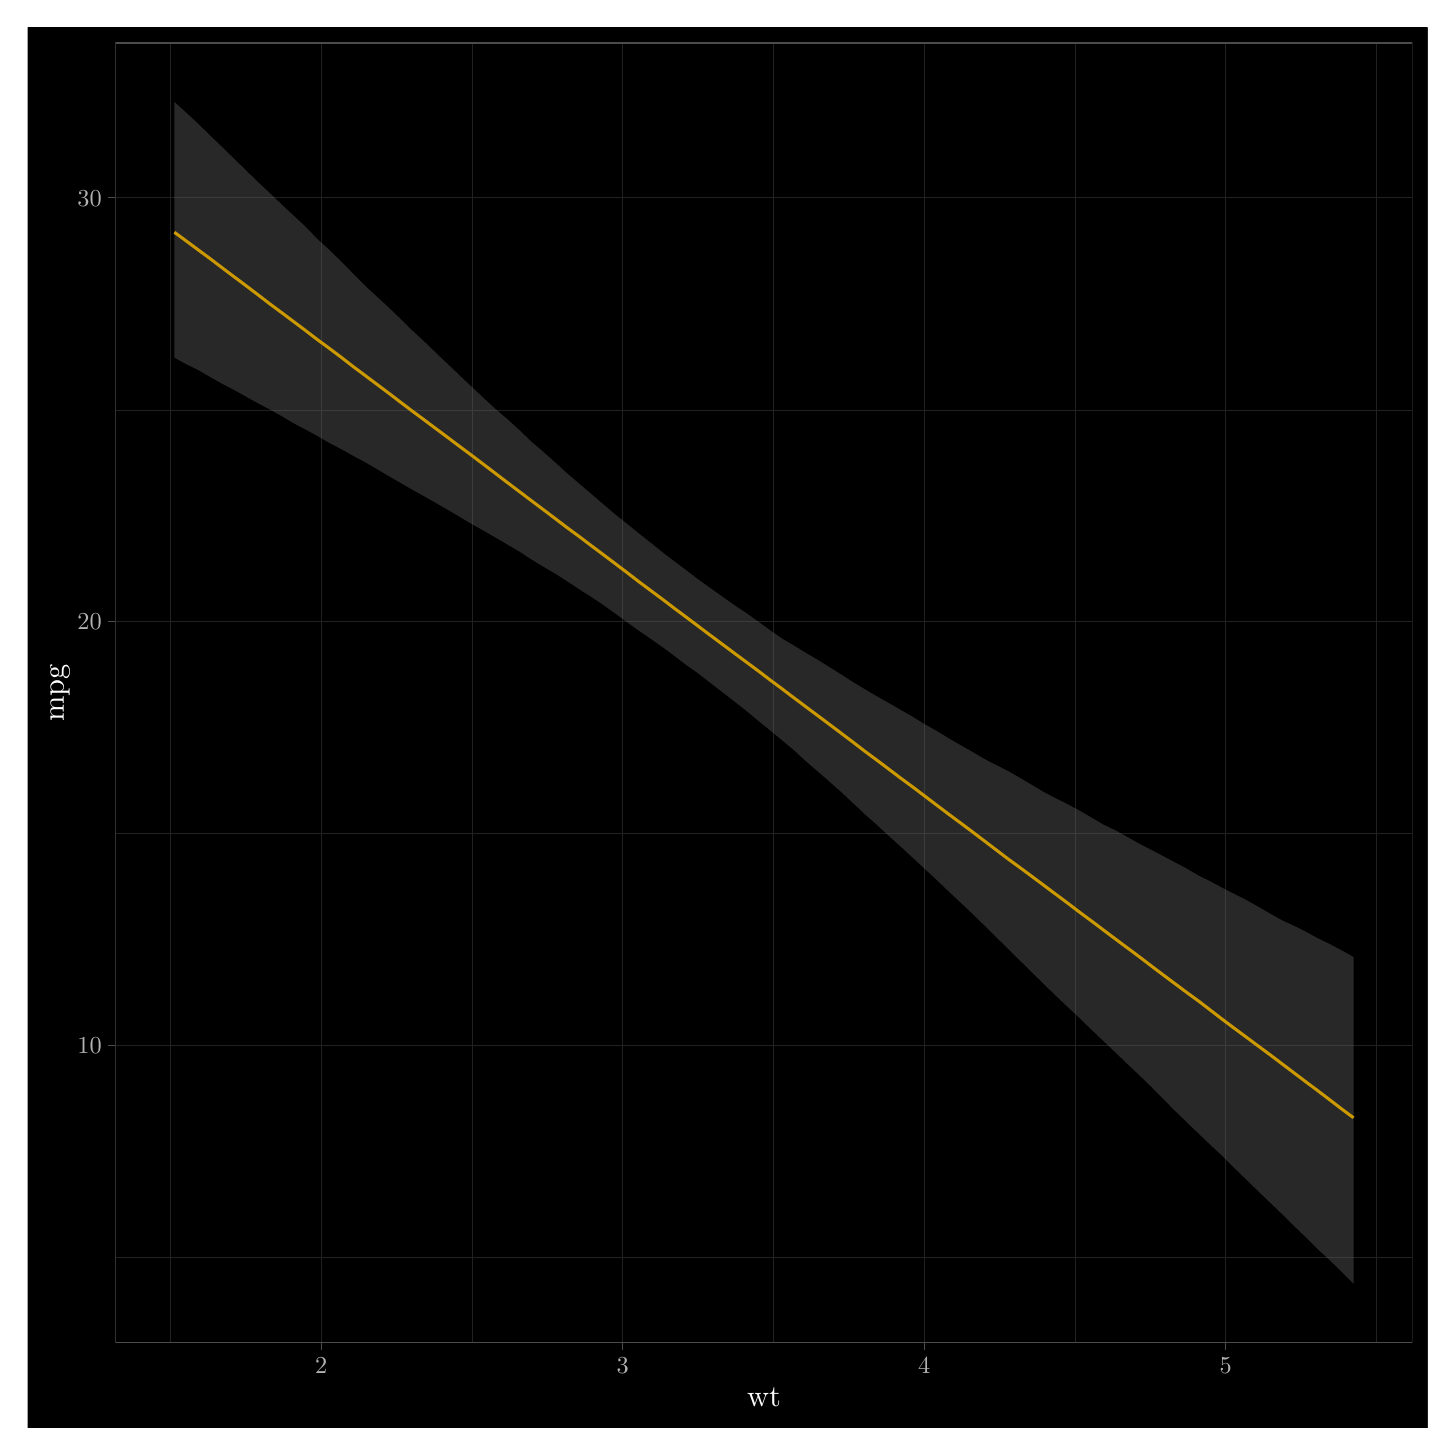
\begin{tikzpicture}[x=1pt,y=1pt]
\definecolor{fillColor}{RGB}{255,255,255}
\path[use as bounding box,fill=fillColor,fill opacity=0.00] (0,0) rectangle (505.89,505.89);
\begin{scope}
\path[clip] (  0.00,  0.00) rectangle (505.89,505.89);
\definecolor{drawColor}{RGB}{0,0,0}
\definecolor{fillColor}{RGB}{0,0,0}

\path[draw=drawColor,line width= 0.6pt,line join=round,line cap=round,fill=fillColor] (  0.00,  0.00) rectangle (505.89,505.89);
\end{scope}
\begin{scope}
\path[clip] ( 31.71, 30.69) rectangle (500.39,500.39);
\definecolor{fillColor}{RGB}{0,0,0}

\path[fill=fillColor] ( 31.71, 30.69) rectangle (500.39,500.39);
\definecolor{drawColor}{gray}{0.13}

\path[draw=drawColor,line width= 0.1pt,line join=round] ( 31.71, 61.51) --
	(500.39, 61.51);

\path[draw=drawColor,line width= 0.1pt,line join=round] ( 31.71,214.68) --
	(500.39,214.68);

\path[draw=drawColor,line width= 0.1pt,line join=round] ( 31.71,367.86) --
	(500.39,367.86);

\path[draw=drawColor,line width= 0.1pt,line join=round] ( 51.60, 30.69) --
	( 51.60,500.39);

\path[draw=drawColor,line width= 0.1pt,line join=round] (160.54, 30.69) --
	(160.54,500.39);

\path[draw=drawColor,line width= 0.1pt,line join=round] (269.48, 30.69) --
	(269.48,500.39);

\path[draw=drawColor,line width= 0.1pt,line join=round] (378.42, 30.69) --
	(378.42,500.39);

\path[draw=drawColor,line width= 0.1pt,line join=round] (487.37, 30.69) --
	(487.37,500.39);

\path[draw=drawColor,line width= 0.3pt,line join=round] ( 31.71,138.10) --
	(500.39,138.10);

\path[draw=drawColor,line width= 0.3pt,line join=round] ( 31.71,291.27) --
	(500.39,291.27);

\path[draw=drawColor,line width= 0.3pt,line join=round] ( 31.71,444.45) --
	(500.39,444.45);

\path[draw=drawColor,line width= 0.3pt,line join=round] (106.07, 30.69) --
	(106.07,500.39);

\path[draw=drawColor,line width= 0.3pt,line join=round] (215.01, 30.69) --
	(215.01,500.39);

\path[draw=drawColor,line width= 0.3pt,line join=round] (323.95, 30.69) --
	(323.95,500.39);

\path[draw=drawColor,line width= 0.3pt,line join=round] (432.90, 30.69) --
	(432.90,500.39);
\definecolor{fillColor}{RGB}{102,102,102}

\path[fill=fillColor,fill opacity=0.40] ( 53.02,479.04) --
	( 57.32,475.13) --
	( 61.62,471.14) --
	( 65.93,466.91) --
	( 70.23,462.77) --
	( 74.53,458.57) --
	( 78.84,454.38) --
	( 83.14,450.16) --
	( 87.45,446.15) --
	( 91.75,442.01) --
	( 96.05,438.00) --
	(100.36,433.99) --
	(104.66,429.51) --
	(108.96,425.60) --
	(113.27,421.37) --
	(117.57,417.03) --
	(121.88,412.64) --
	(126.18,408.68) --
	(130.48,404.71) --
	(134.79,400.58) --
	(139.09,396.33) --
	(143.39,392.38) --
	(147.70,388.21) --
	(152.00,384.12) --
	(156.31,380.00) --
	(160.61,375.93) --
	(164.91,371.90) --
	(169.22,367.92) --
	(173.52,364.26) --
	(177.82,360.33) --
	(182.13,356.17) --
	(186.43,352.51) --
	(190.74,348.65) --
	(195.04,344.75) --
	(199.34,341.06) --
	(203.65,337.40) --
	(207.95,333.69) --
	(212.25,330.04) --
	(216.56,326.60) --
	(220.86,323.13) --
	(225.17,319.71) --
	(229.47,316.25) --
	(233.77,312.95) --
	(238.08,309.74) --
	(242.38,306.45) --
	(246.68,303.37) --
	(250.99,300.30) --
	(255.29,297.25) --
	(259.60,294.39) --
	(263.90,291.33) --
	(268.20,288.19) --
	(272.51,285.19) --
	(276.81,282.66) --
	(281.11,280.01) --
	(285.42,277.48) --
	(289.72,274.80) --
	(294.03,272.10) --
	(298.33,269.34) --
	(302.63,266.75) --
	(306.94,264.20) --
	(311.24,261.81) --
	(315.54,259.31) --
	(319.85,256.84) --
	(324.15,254.17) --
	(328.46,251.75) --
	(332.76,249.12) --
	(337.06,246.63) --
	(341.37,244.20) --
	(345.67,241.63) --
	(349.97,239.43) --
	(354.28,237.25) --
	(358.58,234.78) --
	(362.89,232.22) --
	(367.19,229.66) --
	(371.49,227.40) --
	(375.80,225.27) --
	(380.10,222.94) --
	(384.40,220.46) --
	(388.71,217.90) --
	(393.01,215.85) --
	(397.32,213.45) --
	(401.62,211.04) --
	(405.92,208.82) --
	(410.23,206.55) --
	(414.53,204.29) --
	(418.83,202.01) --
	(423.14,199.47) --
	(427.44,197.36) --
	(431.75,195.02) --
	(436.05,192.81) --
	(440.35,190.67) --
	(444.66,188.21) --
	(448.96,185.74) --
	(453.26,183.33) --
	(457.57,181.33) --
	(461.87,179.20) --
	(466.18,176.83) --
	(470.48,174.76) --
	(474.78,172.48) --
	(479.09,170.07) --
	(479.09, 52.04) --
	(474.78, 56.39) --
	(470.48, 60.56) --
	(466.18, 64.49) --
	(461.87, 68.81) --
	(457.57, 72.94) --
	(453.26, 77.22) --
	(448.96, 81.34) --
	(444.66, 85.46) --
	(440.35, 89.69) --
	(436.05, 93.83) --
	(431.75, 98.12) --
	(427.44,102.15) --
	(423.14,106.27) --
	(418.83,110.41) --
	(414.53,114.56) --
	(410.23,118.88) --
	(405.92,123.28) --
	(401.62,127.45) --
	(397.32,131.51) --
	(393.01,135.65) --
	(388.71,139.72) --
	(384.40,143.84) --
	(380.10,148.02) --
	(375.80,152.05) --
	(371.49,156.13) --
	(367.19,160.31) --
	(362.89,164.55) --
	(358.58,168.79) --
	(354.28,173.03) --
	(349.97,177.31) --
	(345.67,181.54) --
	(341.37,185.78) --
	(337.06,189.79) --
	(332.76,193.83) --
	(328.46,197.95) --
	(324.15,201.95) --
	(319.85,205.94) --
	(315.54,209.93) --
	(311.24,213.80) --
	(306.94,217.77) --
	(302.63,221.58) --
	(298.33,225.62) --
	(294.03,229.67) --
	(289.72,233.48) --
	(285.42,237.22) --
	(281.11,240.93) --
	(276.81,244.90) --
	(272.51,248.49) --
	(268.20,252.05) --
	(263.90,255.53) --
	(259.60,259.14) --
	(255.29,262.48) --
	(250.99,265.83) --
	(246.68,269.16) --
	(242.38,272.51) --
	(238.08,275.53) --
	(233.77,278.81) --
	(229.47,282.04) --
	(225.17,285.04) --
	(220.86,287.98) --
	(216.56,291.11) --
	(212.25,294.25) --
	(207.95,297.36) --
	(203.65,300.21) --
	(199.34,302.95) --
	(195.04,305.80) --
	(190.74,308.56) --
	(186.43,311.07) --
	(182.13,313.69) --
	(177.82,316.51) --
	(173.52,319.05) --
	(169.22,321.56) --
	(164.91,324.04) --
	(160.61,326.47) --
	(156.31,329.04) --
	(152.00,331.56) --
	(147.70,334.06) --
	(143.39,336.50) --
	(139.09,338.88) --
	(134.79,341.39) --
	(130.48,343.86) --
	(126.18,346.40) --
	(121.88,348.92) --
	(117.57,351.22) --
	(113.27,353.64) --
	(108.96,355.86) --
	(104.66,358.39) --
	(100.36,360.71) --
	( 96.05,362.99) --
	( 91.75,365.55) --
	( 87.45,367.97) --
	( 83.14,370.21) --
	( 78.84,372.63) --
	( 74.53,375.01) --
	( 70.23,377.25) --
	( 65.93,379.69) --
	( 61.62,382.18) --
	( 57.32,384.29) --
	( 53.02,386.68) --
	cycle;

\path[] ( 53.02,479.04) --
	( 57.32,475.13) --
	( 61.62,471.14) --
	( 65.93,466.91) --
	( 70.23,462.77) --
	( 74.53,458.57) --
	( 78.84,454.38) --
	( 83.14,450.16) --
	( 87.45,446.15) --
	( 91.75,442.01) --
	( 96.05,438.00) --
	(100.36,433.99) --
	(104.66,429.51) --
	(108.96,425.60) --
	(113.27,421.37) --
	(117.57,417.03) --
	(121.88,412.64) --
	(126.18,408.68) --
	(130.48,404.71) --
	(134.79,400.58) --
	(139.09,396.33) --
	(143.39,392.38) --
	(147.70,388.21) --
	(152.00,384.12) --
	(156.31,380.00) --
	(160.61,375.93) --
	(164.91,371.90) --
	(169.22,367.92) --
	(173.52,364.26) --
	(177.82,360.33) --
	(182.13,356.17) --
	(186.43,352.51) --
	(190.74,348.65) --
	(195.04,344.75) --
	(199.34,341.06) --
	(203.65,337.40) --
	(207.95,333.69) --
	(212.25,330.04) --
	(216.56,326.60) --
	(220.86,323.13) --
	(225.17,319.71) --
	(229.47,316.25) --
	(233.77,312.95) --
	(238.08,309.74) --
	(242.38,306.45) --
	(246.68,303.37) --
	(250.99,300.30) --
	(255.29,297.25) --
	(259.60,294.39) --
	(263.90,291.33) --
	(268.20,288.19) --
	(272.51,285.19) --
	(276.81,282.66) --
	(281.11,280.01) --
	(285.42,277.48) --
	(289.72,274.80) --
	(294.03,272.10) --
	(298.33,269.34) --
	(302.63,266.75) --
	(306.94,264.20) --
	(311.24,261.81) --
	(315.54,259.31) --
	(319.85,256.84) --
	(324.15,254.17) --
	(328.46,251.75) --
	(332.76,249.12) --
	(337.06,246.63) --
	(341.37,244.20) --
	(345.67,241.63) --
	(349.97,239.43) --
	(354.28,237.25) --
	(358.58,234.78) --
	(362.89,232.22) --
	(367.19,229.66) --
	(371.49,227.40) --
	(375.80,225.27) --
	(380.10,222.94) --
	(384.40,220.46) --
	(388.71,217.90) --
	(393.01,215.85) --
	(397.32,213.45) --
	(401.62,211.04) --
	(405.92,208.82) --
	(410.23,206.55) --
	(414.53,204.29) --
	(418.83,202.01) --
	(423.14,199.47) --
	(427.44,197.36) --
	(431.75,195.02) --
	(436.05,192.81) --
	(440.35,190.67) --
	(444.66,188.21) --
	(448.96,185.74) --
	(453.26,183.33) --
	(457.57,181.33) --
	(461.87,179.20) --
	(466.18,176.83) --
	(470.48,174.76) --
	(474.78,172.48) --
	(479.09,170.07);

\path[] (479.09, 52.04) --
	(474.78, 56.39) --
	(470.48, 60.56) --
	(466.18, 64.49) --
	(461.87, 68.81) --
	(457.57, 72.94) --
	(453.26, 77.22) --
	(448.96, 81.34) --
	(444.66, 85.46) --
	(440.35, 89.69) --
	(436.05, 93.83) --
	(431.75, 98.12) --
	(427.44,102.15) --
	(423.14,106.27) --
	(418.83,110.41) --
	(414.53,114.56) --
	(410.23,118.88) --
	(405.92,123.28) --
	(401.62,127.45) --
	(397.32,131.51) --
	(393.01,135.65) --
	(388.71,139.72) --
	(384.40,143.84) --
	(380.10,148.02) --
	(375.80,152.05) --
	(371.49,156.13) --
	(367.19,160.31) --
	(362.89,164.55) --
	(358.58,168.79) --
	(354.28,173.03) --
	(349.97,177.31) --
	(345.67,181.54) --
	(341.37,185.78) --
	(337.06,189.79) --
	(332.76,193.83) --
	(328.46,197.95) --
	(324.15,201.95) --
	(319.85,205.94) --
	(315.54,209.93) --
	(311.24,213.80) --
	(306.94,217.77) --
	(302.63,221.58) --
	(298.33,225.62) --
	(294.03,229.67) --
	(289.72,233.48) --
	(285.42,237.22) --
	(281.11,240.93) --
	(276.81,244.90) --
	(272.51,248.49) --
	(268.20,252.05) --
	(263.90,255.53) --
	(259.60,259.14) --
	(255.29,262.48) --
	(250.99,265.83) --
	(246.68,269.16) --
	(242.38,272.51) --
	(238.08,275.53) --
	(233.77,278.81) --
	(229.47,282.04) --
	(225.17,285.04) --
	(220.86,287.98) --
	(216.56,291.11) --
	(212.25,294.25) --
	(207.95,297.36) --
	(203.65,300.21) --
	(199.34,302.95) --
	(195.04,305.80) --
	(190.74,308.56) --
	(186.43,311.07) --
	(182.13,313.69) --
	(177.82,316.51) --
	(173.52,319.05) --
	(169.22,321.56) --
	(164.91,324.04) --
	(160.61,326.47) --
	(156.31,329.04) --
	(152.00,331.56) --
	(147.70,334.06) --
	(143.39,336.50) --
	(139.09,338.88) --
	(134.79,341.39) --
	(130.48,343.86) --
	(126.18,346.40) --
	(121.88,348.92) --
	(117.57,351.22) --
	(113.27,353.64) --
	(108.96,355.86) --
	(104.66,358.39) --
	(100.36,360.71) --
	( 96.05,362.99) --
	( 91.75,365.55) --
	( 87.45,367.97) --
	( 83.14,370.21) --
	( 78.84,372.63) --
	( 74.53,375.01) --
	( 70.23,377.25) --
	( 65.93,379.69) --
	( 61.62,382.18) --
	( 57.32,384.29) --
	( 53.02,386.68);
\definecolor{drawColor}{RGB}{204,153,0}

\path[draw=drawColor,line width= 1.1pt,line join=round] ( 53.02,431.96) --
	( 57.32,428.79) --
	( 61.62,425.60) --
	( 65.93,422.42) --
	( 70.23,419.16) --
	( 74.53,415.91) --
	( 78.84,412.69) --
	( 83.14,409.43) --
	( 87.45,406.12) --
	( 91.75,402.93) --
	( 96.05,399.72) --
	(100.36,396.48) --
	(104.66,393.18) --
	(108.96,390.04) --
	(113.27,386.80) --
	(117.57,383.46) --
	(121.88,380.25) --
	(126.18,377.02) --
	(130.48,373.81) --
	(134.79,370.50) --
	(139.09,367.26) --
	(143.39,364.08) --
	(147.70,360.85) --
	(152.00,357.65) --
	(156.31,354.41) --
	(160.61,351.20) --
	(164.91,347.95) --
	(169.22,344.67) --
	(173.52,341.38) --
	(177.82,338.14) --
	(182.13,334.88) --
	(186.43,331.66) --
	(190.74,328.40) --
	(195.04,325.13) --
	(199.34,321.98) --
	(203.65,318.71) --
	(207.95,315.49) --
	(212.25,312.26) --
	(216.56,309.01) --
	(220.86,305.68) --
	(225.17,302.47) --
	(229.47,299.28) --
	(233.77,296.00) --
	(238.08,292.79) --
	(242.38,289.55) --
	(246.68,286.32) --
	(250.99,283.11) --
	(255.29,279.90) --
	(259.60,276.71) --
	(263.90,273.52) --
	(268.20,270.24) --
	(272.51,267.05) --
	(276.81,263.78) --
	(281.11,260.55) --
	(285.42,257.35) --
	(289.72,254.13) --
	(294.03,250.88) --
	(298.33,247.63) --
	(302.63,244.33) --
	(306.94,241.14) --
	(311.24,237.90) --
	(315.54,234.65) --
	(319.85,231.48) --
	(324.15,228.23) --
	(328.46,224.96) --
	(332.76,221.71) --
	(337.06,218.52) --
	(341.37,215.31) --
	(345.67,212.04) --
	(349.97,208.78) --
	(354.28,205.49) --
	(358.58,202.37) --
	(362.89,199.18) --
	(367.19,195.97) --
	(371.49,192.76) --
	(375.80,189.55) --
	(380.10,186.26) --
	(384.40,183.09) --
	(388.71,179.84) --
	(393.01,176.60) --
	(397.32,173.40) --
	(401.62,170.21) --
	(405.92,166.92) --
	(410.23,163.66) --
	(414.53,160.46) --
	(418.83,157.26) --
	(423.14,154.12) --
	(427.44,150.82) --
	(431.75,147.50) --
	(436.05,144.29) --
	(440.35,141.11) --
	(444.66,137.91) --
	(448.96,134.73) --
	(453.26,131.47) --
	(457.57,128.22) --
	(461.87,124.97) --
	(466.18,121.75) --
	(470.48,118.48) --
	(474.78,115.18) --
	(479.09,111.98);
\definecolor{drawColor}{RGB}{76,76,76}

\path[draw=drawColor,line width= 0.6pt,line join=round,line cap=round] ( 31.71, 30.69) rectangle (500.39,500.39);
\end{scope}
\begin{scope}
\path[clip] (  0.00,  0.00) rectangle (505.89,505.89);
\definecolor{drawColor}{RGB}{178,178,178}

\node[text=drawColor,anchor=base east,inner sep=0pt, outer sep=0pt, scale=  0.88] at ( 26.76,135.07) {10};

\node[text=drawColor,anchor=base east,inner sep=0pt, outer sep=0pt, scale=  0.88] at ( 26.76,288.24) {20};

\node[text=drawColor,anchor=base east,inner sep=0pt, outer sep=0pt, scale=  0.88] at ( 26.76,441.42) {30};
\end{scope}
\begin{scope}
\path[clip] (  0.00,  0.00) rectangle (505.89,505.89);
\definecolor{drawColor}{RGB}{76,76,76}

\path[draw=drawColor,line width= 0.3pt,line join=round] ( 28.96,138.10) --
	( 31.71,138.10);

\path[draw=drawColor,line width= 0.3pt,line join=round] ( 28.96,291.27) --
	( 31.71,291.27);

\path[draw=drawColor,line width= 0.3pt,line join=round] ( 28.96,444.45) --
	( 31.71,444.45);
\end{scope}
\begin{scope}
\path[clip] (  0.00,  0.00) rectangle (505.89,505.89);
\definecolor{drawColor}{RGB}{76,76,76}

\path[draw=drawColor,line width= 0.3pt,line join=round] (106.07, 27.94) --
	(106.07, 30.69);

\path[draw=drawColor,line width= 0.3pt,line join=round] (215.01, 27.94) --
	(215.01, 30.69);

\path[draw=drawColor,line width= 0.3pt,line join=round] (323.95, 27.94) --
	(323.95, 30.69);

\path[draw=drawColor,line width= 0.3pt,line join=round] (432.90, 27.94) --
	(432.90, 30.69);
\end{scope}
\begin{scope}
\path[clip] (  0.00,  0.00) rectangle (505.89,505.89);
\definecolor{drawColor}{RGB}{178,178,178}

\node[text=drawColor,anchor=base,inner sep=0pt, outer sep=0pt, scale=  0.88] at (106.07, 19.68) {2};

\node[text=drawColor,anchor=base,inner sep=0pt, outer sep=0pt, scale=  0.88] at (215.01, 19.68) {3};

\node[text=drawColor,anchor=base,inner sep=0pt, outer sep=0pt, scale=  0.88] at (323.95, 19.68) {4};

\node[text=drawColor,anchor=base,inner sep=0pt, outer sep=0pt, scale=  0.88] at (432.90, 19.68) {5};
\end{scope}
\begin{scope}
\path[clip] (  0.00,  0.00) rectangle (505.89,505.89);
\definecolor{drawColor}{RGB}{255,255,255}

\node[text=drawColor,anchor=base,inner sep=0pt, outer sep=0pt, scale=  1.10] at (266.05,  7.64) {wt};
\end{scope}
\begin{scope}
\path[clip] (  0.00,  0.00) rectangle (505.89,505.89);
\definecolor{drawColor}{RGB}{255,255,255}

\node[text=drawColor,rotate= 90.00,anchor=base,inner sep=0pt, outer sep=0pt, scale=  1.10] at ( 13.08,265.54) {mpg};
\end{scope}
\end{tikzpicture}
}
			\end{figure}
		\end{column}
		\begin{column}{0.5\textwidth}
			\centering
			\begin{figure}
				\resizebox{0.9\linewidth}{!}{% Created by tikzDevice version 0.12.3.1 on 2021-05-28 17:03:18
% !TEX encoding = UTF-8 Unicode
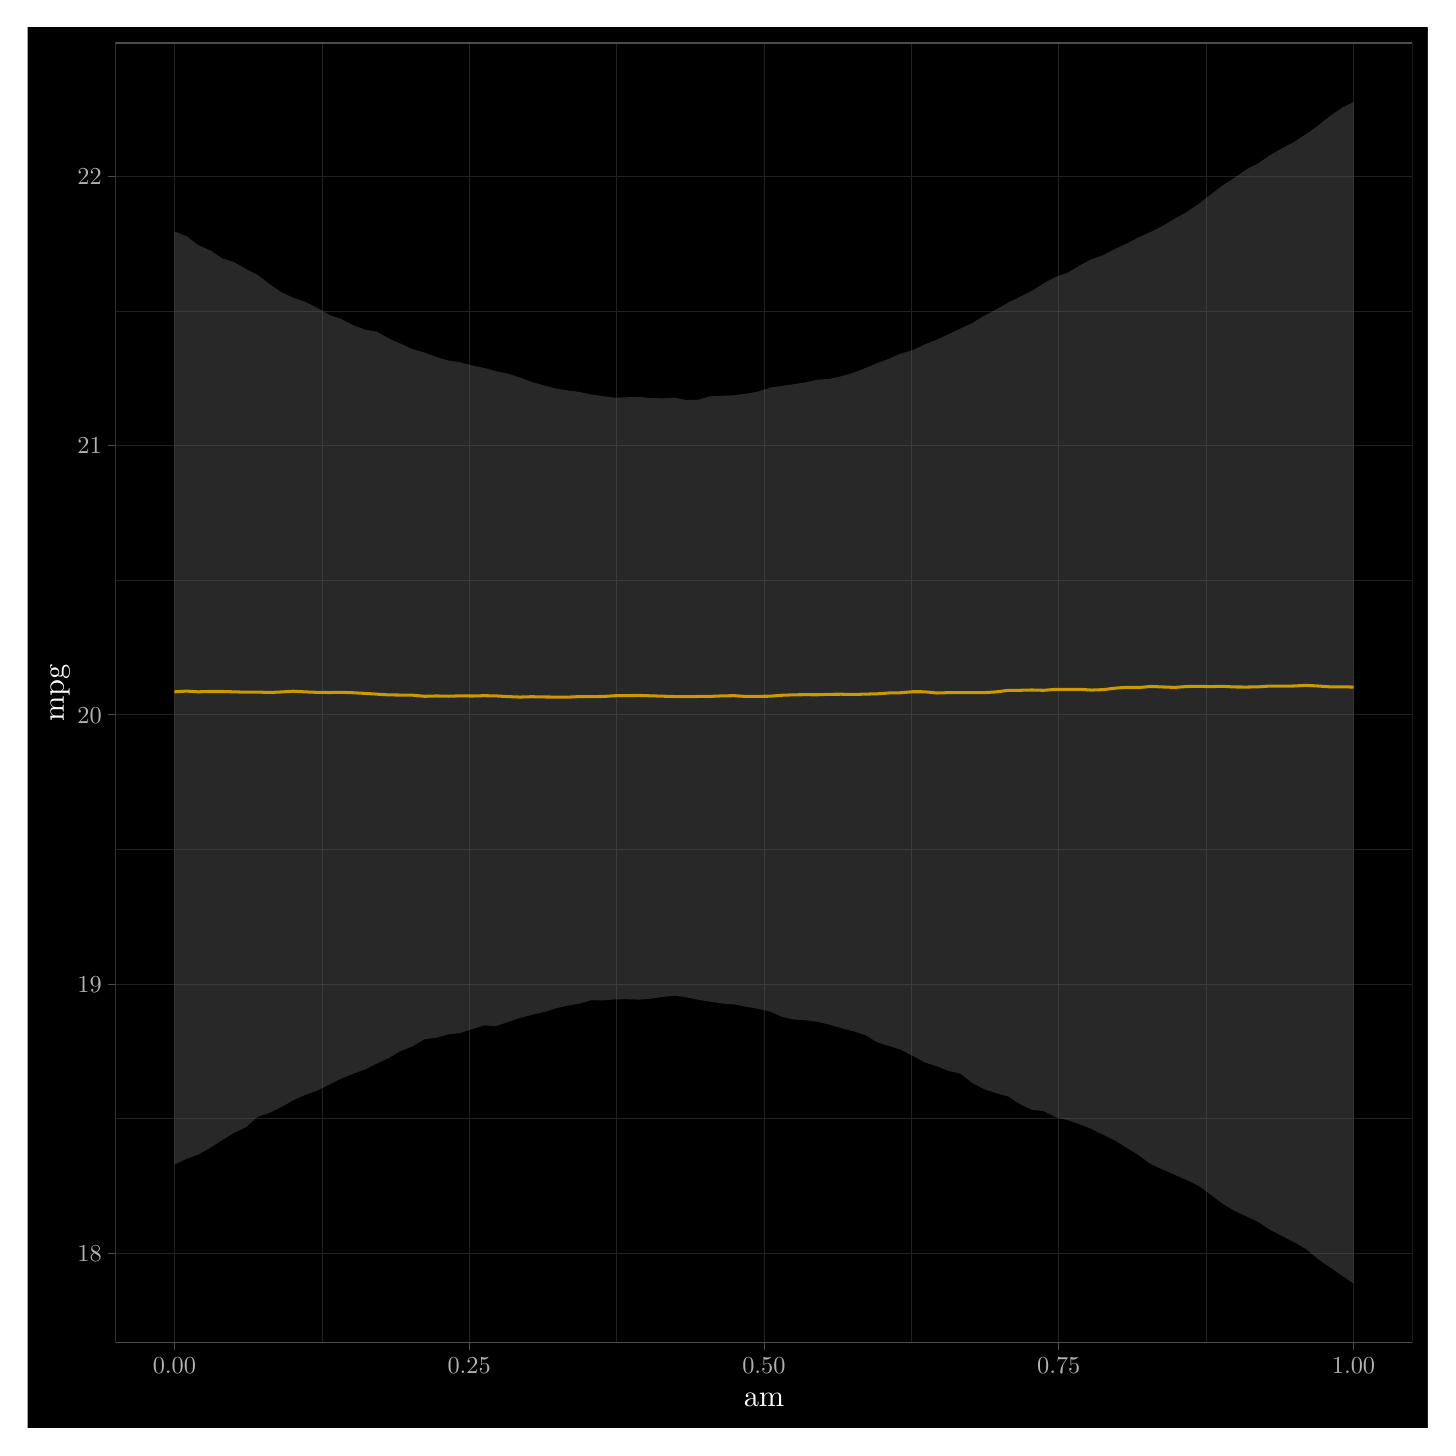
\begin{tikzpicture}[x=1pt,y=1pt]
\definecolor{fillColor}{RGB}{255,255,255}
\path[use as bounding box,fill=fillColor,fill opacity=0.00] (0,0) rectangle (505.89,505.89);
\begin{scope}
\path[clip] (  0.00,  0.00) rectangle (505.89,505.89);
\definecolor{drawColor}{RGB}{0,0,0}
\definecolor{fillColor}{RGB}{0,0,0}

\path[draw=drawColor,line width= 0.6pt,line join=round,line cap=round,fill=fillColor] (  0.00,  0.00) rectangle (505.89,505.89);
\end{scope}
\begin{scope}
\path[clip] ( 31.71, 30.69) rectangle (500.39,500.39);
\definecolor{fillColor}{RGB}{0,0,0}

\path[fill=fillColor] ( 31.71, 30.69) rectangle (500.39,500.39);
\definecolor{drawColor}{gray}{0.13}

\path[draw=drawColor,line width= 0.1pt,line join=round] ( 31.71,111.68) --
	(500.39,111.68);

\path[draw=drawColor,line width= 0.1pt,line join=round] ( 31.71,208.99) --
	(500.39,208.99);

\path[draw=drawColor,line width= 0.1pt,line join=round] ( 31.71,306.29) --
	(500.39,306.29);

\path[draw=drawColor,line width= 0.1pt,line join=round] ( 31.71,403.60) --
	(500.39,403.60);

\path[draw=drawColor,line width= 0.1pt,line join=round] (106.27, 30.69) --
	(106.27,500.39);

\path[draw=drawColor,line width= 0.1pt,line join=round] (212.79, 30.69) --
	(212.79,500.39);

\path[draw=drawColor,line width= 0.1pt,line join=round] (319.31, 30.69) --
	(319.31,500.39);

\path[draw=drawColor,line width= 0.1pt,line join=round] (425.83, 30.69) --
	(425.83,500.39);

\path[draw=drawColor,line width= 0.3pt,line join=round] ( 31.71, 63.03) --
	(500.39, 63.03);

\path[draw=drawColor,line width= 0.3pt,line join=round] ( 31.71,160.33) --
	(500.39,160.33);

\path[draw=drawColor,line width= 0.3pt,line join=round] ( 31.71,257.64) --
	(500.39,257.64);

\path[draw=drawColor,line width= 0.3pt,line join=round] ( 31.71,354.95) --
	(500.39,354.95);

\path[draw=drawColor,line width= 0.3pt,line join=round] ( 31.71,452.26) --
	(500.39,452.26);

\path[draw=drawColor,line width= 0.3pt,line join=round] ( 53.02, 30.69) --
	( 53.02,500.39);

\path[draw=drawColor,line width= 0.3pt,line join=round] (159.53, 30.69) --
	(159.53,500.39);

\path[draw=drawColor,line width= 0.3pt,line join=round] (266.05, 30.69) --
	(266.05,500.39);

\path[draw=drawColor,line width= 0.3pt,line join=round] (372.57, 30.69) --
	(372.57,500.39);

\path[draw=drawColor,line width= 0.3pt,line join=round] (479.09, 30.69) --
	(479.09,500.39);
\definecolor{fillColor}{RGB}{102,102,102}

\path[fill=fillColor,fill opacity=0.40] ( 53.02,432.24) --
	( 57.32,430.56) --
	( 61.62,427.34) --
	( 65.93,425.41) --
	( 70.23,422.54) --
	( 74.53,421.19) --
	( 78.84,418.70) --
	( 83.14,416.54) --
	( 87.45,413.16) --
	( 91.75,410.25) --
	( 96.05,408.24) --
	(100.36,406.82) --
	(104.66,404.65) --
	(108.96,402.10) --
	(113.27,400.64) --
	(117.57,398.36) --
	(121.88,396.78) --
	(126.18,396.00) --
	(130.48,393.60) --
	(134.79,391.69) --
	(139.09,389.71) --
	(143.39,388.52) --
	(147.70,386.81) --
	(152.00,385.63) --
	(156.31,384.97) --
	(160.61,383.79) --
	(164.91,382.95) --
	(169.22,381.72) --
	(173.52,380.87) --
	(177.82,379.48) --
	(182.13,377.87) --
	(186.43,376.67) --
	(190.74,375.50) --
	(195.04,374.82) --
	(199.34,374.24) --
	(203.65,373.34) --
	(207.95,372.74) --
	(212.25,372.15) --
	(216.56,372.33) --
	(220.86,372.45) --
	(225.17,372.06) --
	(229.47,371.94) --
	(233.77,372.17) --
	(238.08,371.32) --
	(242.38,371.46) --
	(246.68,372.69) --
	(250.99,372.83) --
	(255.29,373.07) --
	(259.60,373.61) --
	(263.90,374.39) --
	(268.20,375.81) --
	(272.51,376.44) --
	(276.81,377.05) --
	(281.11,377.72) --
	(285.42,378.68) --
	(289.72,378.96) --
	(294.03,379.93) --
	(298.33,381.14) --
	(302.63,382.86) --
	(306.94,384.62) --
	(311.24,386.23) --
	(315.54,388.13) --
	(319.85,389.38) --
	(324.15,391.43) --
	(328.46,393.10) --
	(332.76,395.13) --
	(337.06,397.16) --
	(341.37,399.18) --
	(345.67,401.77) --
	(349.97,404.05) --
	(354.28,406.53) --
	(358.58,408.63) --
	(362.89,410.78) --
	(367.19,413.54) --
	(371.49,415.84) --
	(375.80,417.31) --
	(380.10,419.92) --
	(384.40,422.22) --
	(388.71,423.70) --
	(393.01,425.96) --
	(397.32,427.96) --
	(401.62,430.18) --
	(405.92,432.13) --
	(410.23,434.27) --
	(414.53,436.89) --
	(418.83,439.28) --
	(423.14,442.16) --
	(427.44,445.58) --
	(431.75,448.83) --
	(436.05,451.58) --
	(440.35,454.63) --
	(444.66,456.86) --
	(448.96,459.85) --
	(453.26,462.33) --
	(457.57,464.57) --
	(461.87,467.38) --
	(466.18,470.41) --
	(470.48,473.88) --
	(474.78,476.83) --
	(479.09,479.04) --
	(479.09, 52.04) --
	(474.78, 55.05) --
	(470.48, 58.01) --
	(466.18, 61.00) --
	(461.87, 64.60) --
	(457.57, 67.02) --
	(453.26, 69.25) --
	(448.96, 71.50) --
	(444.66, 74.36) --
	(440.35, 76.35) --
	(436.05, 78.36) --
	(431.75, 80.96) --
	(427.44, 84.23) --
	(423.14, 87.38) --
	(418.83, 89.45) --
	(414.53, 91.36) --
	(410.23, 93.24) --
	(405.92, 95.18) --
	(401.62, 98.33) --
	(397.32,101.01) --
	(393.01,103.71) --
	(388.71,105.83) --
	(384.40,107.94) --
	(380.10,109.68) --
	(375.80,111.12) --
	(371.49,112.14) --
	(367.19,114.38) --
	(362.89,114.83) --
	(358.58,116.94) --
	(354.28,119.69) --
	(349.97,120.86) --
	(345.67,122.28) --
	(341.37,124.57) --
	(337.06,127.91) --
	(332.76,128.91) --
	(328.46,130.60) --
	(324.15,131.99) --
	(319.85,134.36) --
	(315.54,136.55) --
	(311.24,137.94) --
	(306.94,139.30) --
	(302.63,141.86) --
	(298.33,143.25) --
	(294.03,144.37) --
	(289.72,145.63) --
	(285.42,146.66) --
	(281.11,147.23) --
	(276.81,147.49) --
	(272.51,148.47) --
	(268.20,150.43) --
	(263.90,151.36) --
	(259.60,152.09) --
	(255.29,152.94) --
	(250.99,153.24) --
	(246.68,153.93) --
	(242.38,154.60) --
	(238.08,155.50) --
	(233.77,156.12) --
	(229.47,155.66) --
	(225.17,155.00) --
	(220.86,154.68) --
	(216.56,154.83) --
	(212.25,154.78) --
	(207.95,154.37) --
	(203.65,154.47) --
	(199.34,153.21) --
	(195.04,152.52) --
	(190.74,151.48) --
	(186.43,150.13) --
	(182.13,149.17) --
	(177.82,148.07) --
	(173.52,146.59) --
	(169.22,145.09) --
	(164.91,145.35) --
	(160.61,144.05) --
	(156.31,142.60) --
	(152.00,142.14) --
	(147.70,140.90) --
	(143.39,140.35) --
	(139.09,137.81) --
	(134.79,136.14) --
	(130.48,133.59) --
	(126.18,131.58) --
	(121.88,129.45) --
	(117.57,127.88) --
	(113.27,126.12) --
	(108.96,123.99) --
	(104.66,121.80) --
	(100.36,120.28) --
	( 96.05,118.34) --
	( 91.75,115.92) --
	( 87.45,113.75) --
	( 83.14,112.34) --
	( 78.84,108.57) --
	( 74.53,106.49) --
	( 70.23,103.86) --
	( 65.93,101.07) --
	( 61.62, 98.69) --
	( 57.32, 97.07) --
	( 53.02, 95.07) --
	cycle;

\path[] ( 53.02,432.24) --
	( 57.32,430.56) --
	( 61.62,427.34) --
	( 65.93,425.41) --
	( 70.23,422.54) --
	( 74.53,421.19) --
	( 78.84,418.70) --
	( 83.14,416.54) --
	( 87.45,413.16) --
	( 91.75,410.25) --
	( 96.05,408.24) --
	(100.36,406.82) --
	(104.66,404.65) --
	(108.96,402.10) --
	(113.27,400.64) --
	(117.57,398.36) --
	(121.88,396.78) --
	(126.18,396.00) --
	(130.48,393.60) --
	(134.79,391.69) --
	(139.09,389.71) --
	(143.39,388.52) --
	(147.70,386.81) --
	(152.00,385.63) --
	(156.31,384.97) --
	(160.61,383.79) --
	(164.91,382.95) --
	(169.22,381.72) --
	(173.52,380.87) --
	(177.82,379.48) --
	(182.13,377.87) --
	(186.43,376.67) --
	(190.74,375.50) --
	(195.04,374.82) --
	(199.34,374.24) --
	(203.65,373.34) --
	(207.95,372.74) --
	(212.25,372.15) --
	(216.56,372.33) --
	(220.86,372.45) --
	(225.17,372.06) --
	(229.47,371.94) --
	(233.77,372.17) --
	(238.08,371.32) --
	(242.38,371.46) --
	(246.68,372.69) --
	(250.99,372.83) --
	(255.29,373.07) --
	(259.60,373.61) --
	(263.90,374.39) --
	(268.20,375.81) --
	(272.51,376.44) --
	(276.81,377.05) --
	(281.11,377.72) --
	(285.42,378.68) --
	(289.72,378.96) --
	(294.03,379.93) --
	(298.33,381.14) --
	(302.63,382.86) --
	(306.94,384.62) --
	(311.24,386.23) --
	(315.54,388.13) --
	(319.85,389.38) --
	(324.15,391.43) --
	(328.46,393.10) --
	(332.76,395.13) --
	(337.06,397.16) --
	(341.37,399.18) --
	(345.67,401.77) --
	(349.97,404.05) --
	(354.28,406.53) --
	(358.58,408.63) --
	(362.89,410.78) --
	(367.19,413.54) --
	(371.49,415.84) --
	(375.80,417.31) --
	(380.10,419.92) --
	(384.40,422.22) --
	(388.71,423.70) --
	(393.01,425.96) --
	(397.32,427.96) --
	(401.62,430.18) --
	(405.92,432.13) --
	(410.23,434.27) --
	(414.53,436.89) --
	(418.83,439.28) --
	(423.14,442.16) --
	(427.44,445.58) --
	(431.75,448.83) --
	(436.05,451.58) --
	(440.35,454.63) --
	(444.66,456.86) --
	(448.96,459.85) --
	(453.26,462.33) --
	(457.57,464.57) --
	(461.87,467.38) --
	(466.18,470.41) --
	(470.48,473.88) --
	(474.78,476.83) --
	(479.09,479.04);

\path[] (479.09, 52.04) --
	(474.78, 55.05) --
	(470.48, 58.01) --
	(466.18, 61.00) --
	(461.87, 64.60) --
	(457.57, 67.02) --
	(453.26, 69.25) --
	(448.96, 71.50) --
	(444.66, 74.36) --
	(440.35, 76.35) --
	(436.05, 78.36) --
	(431.75, 80.96) --
	(427.44, 84.23) --
	(423.14, 87.38) --
	(418.83, 89.45) --
	(414.53, 91.36) --
	(410.23, 93.24) --
	(405.92, 95.18) --
	(401.62, 98.33) --
	(397.32,101.01) --
	(393.01,103.71) --
	(388.71,105.83) --
	(384.40,107.94) --
	(380.10,109.68) --
	(375.80,111.12) --
	(371.49,112.14) --
	(367.19,114.38) --
	(362.89,114.83) --
	(358.58,116.94) --
	(354.28,119.69) --
	(349.97,120.86) --
	(345.67,122.28) --
	(341.37,124.57) --
	(337.06,127.91) --
	(332.76,128.91) --
	(328.46,130.60) --
	(324.15,131.99) --
	(319.85,134.36) --
	(315.54,136.55) --
	(311.24,137.94) --
	(306.94,139.30) --
	(302.63,141.86) --
	(298.33,143.25) --
	(294.03,144.37) --
	(289.72,145.63) --
	(285.42,146.66) --
	(281.11,147.23) --
	(276.81,147.49) --
	(272.51,148.47) --
	(268.20,150.43) --
	(263.90,151.36) --
	(259.60,152.09) --
	(255.29,152.94) --
	(250.99,153.24) --
	(246.68,153.93) --
	(242.38,154.60) --
	(238.08,155.50) --
	(233.77,156.12) --
	(229.47,155.66) --
	(225.17,155.00) --
	(220.86,154.68) --
	(216.56,154.83) --
	(212.25,154.78) --
	(207.95,154.37) --
	(203.65,154.47) --
	(199.34,153.21) --
	(195.04,152.52) --
	(190.74,151.48) --
	(186.43,150.13) --
	(182.13,149.17) --
	(177.82,148.07) --
	(173.52,146.59) --
	(169.22,145.09) --
	(164.91,145.35) --
	(160.61,144.05) --
	(156.31,142.60) --
	(152.00,142.14) --
	(147.70,140.90) --
	(143.39,140.35) --
	(139.09,137.81) --
	(134.79,136.14) --
	(130.48,133.59) --
	(126.18,131.58) --
	(121.88,129.45) --
	(117.57,127.88) --
	(113.27,126.12) --
	(108.96,123.99) --
	(104.66,121.80) --
	(100.36,120.28) --
	( 96.05,118.34) --
	( 91.75,115.92) --
	( 87.45,113.75) --
	( 83.14,112.34) --
	( 78.84,108.57) --
	( 74.53,106.49) --
	( 70.23,103.86) --
	( 65.93,101.07) --
	( 61.62, 98.69) --
	( 57.32, 97.07) --
	( 53.02, 95.07);
\definecolor{drawColor}{RGB}{204,153,0}

\path[draw=drawColor,line width= 1.1pt,line join=round] ( 53.02,265.89) --
	( 57.32,266.16) --
	( 61.62,265.90) --
	( 65.93,266.02) --
	( 70.23,266.02) --
	( 74.53,265.89) --
	( 78.84,265.76) --
	( 83.14,265.80) --
	( 87.45,265.65) --
	( 91.75,265.85) --
	( 96.05,266.12) --
	(100.36,265.87) --
	(104.66,265.70) --
	(108.96,265.64) --
	(113.27,265.73) --
	(117.57,265.56) --
	(121.88,265.33) --
	(126.18,265.06) --
	(130.48,264.78) --
	(134.79,264.73) --
	(139.09,264.69) --
	(143.39,264.28) --
	(147.70,264.40) --
	(152.00,264.30) --
	(156.31,264.44) --
	(160.61,264.38) --
	(164.91,264.50) --
	(169.22,264.42) --
	(173.52,264.17) --
	(177.82,264.00) --
	(182.13,264.13) --
	(186.43,264.04) --
	(190.74,264.00) --
	(195.04,263.96) --
	(199.34,264.17) --
	(203.65,264.17) --
	(207.95,264.22) --
	(212.25,264.48) --
	(216.56,264.53) --
	(220.86,264.59) --
	(225.17,264.45) --
	(229.47,264.32) --
	(233.77,264.19) --
	(238.08,264.14) --
	(242.38,264.22) --
	(246.68,264.24) --
	(250.99,264.43) --
	(255.29,264.50) --
	(259.60,264.22) --
	(263.90,264.27) --
	(268.20,264.31) --
	(272.51,264.65) --
	(276.81,264.81) --
	(281.11,264.86) --
	(285.42,264.83) --
	(289.72,265.00) --
	(294.03,265.03) --
	(298.33,264.93) --
	(302.63,265.07) --
	(306.94,265.17) --
	(311.24,265.48) --
	(315.54,265.56) --
	(319.85,265.93) --
	(324.15,265.91) --
	(328.46,265.47) --
	(332.76,265.59) --
	(337.06,265.63) --
	(341.37,265.61) --
	(345.67,265.61) --
	(349.97,265.87) --
	(354.28,266.43) --
	(358.58,266.45) --
	(362.89,266.56) --
	(367.19,266.44) --
	(371.49,266.80) --
	(375.80,266.76) --
	(380.10,266.81) --
	(384.40,266.53) --
	(388.71,266.69) --
	(393.01,267.23) --
	(397.32,267.53) --
	(401.62,267.46) --
	(405.92,267.83) --
	(410.23,267.65) --
	(414.53,267.49) --
	(418.83,267.81) --
	(423.14,267.88) --
	(427.44,267.77) --
	(431.75,267.89) --
	(436.05,267.65) --
	(440.35,267.62) --
	(444.66,267.69) --
	(448.96,267.99) --
	(453.26,267.94) --
	(457.57,268.00) --
	(461.87,268.24) --
	(466.18,268.00) --
	(470.48,267.70) --
	(474.78,267.71) --
	(479.09,267.61);
\definecolor{drawColor}{RGB}{76,76,76}

\path[draw=drawColor,line width= 0.6pt,line join=round,line cap=round] ( 31.71, 30.69) rectangle (500.39,500.39);
\end{scope}
\begin{scope}
\path[clip] (  0.00,  0.00) rectangle (505.89,505.89);
\definecolor{drawColor}{RGB}{178,178,178}

\node[text=drawColor,anchor=base east,inner sep=0pt, outer sep=0pt, scale=  0.88] at ( 26.76, 60.00) {18};

\node[text=drawColor,anchor=base east,inner sep=0pt, outer sep=0pt, scale=  0.88] at ( 26.76,157.30) {19};

\node[text=drawColor,anchor=base east,inner sep=0pt, outer sep=0pt, scale=  0.88] at ( 26.76,254.61) {20};

\node[text=drawColor,anchor=base east,inner sep=0pt, outer sep=0pt, scale=  0.88] at ( 26.76,351.92) {21};

\node[text=drawColor,anchor=base east,inner sep=0pt, outer sep=0pt, scale=  0.88] at ( 26.76,449.23) {22};
\end{scope}
\begin{scope}
\path[clip] (  0.00,  0.00) rectangle (505.89,505.89);
\definecolor{drawColor}{RGB}{76,76,76}

\path[draw=drawColor,line width= 0.3pt,line join=round] ( 28.96, 63.03) --
	( 31.71, 63.03);

\path[draw=drawColor,line width= 0.3pt,line join=round] ( 28.96,160.33) --
	( 31.71,160.33);

\path[draw=drawColor,line width= 0.3pt,line join=round] ( 28.96,257.64) --
	( 31.71,257.64);

\path[draw=drawColor,line width= 0.3pt,line join=round] ( 28.96,354.95) --
	( 31.71,354.95);

\path[draw=drawColor,line width= 0.3pt,line join=round] ( 28.96,452.26) --
	( 31.71,452.26);
\end{scope}
\begin{scope}
\path[clip] (  0.00,  0.00) rectangle (505.89,505.89);
\definecolor{drawColor}{RGB}{76,76,76}

\path[draw=drawColor,line width= 0.3pt,line join=round] ( 53.02, 27.94) --
	( 53.02, 30.69);

\path[draw=drawColor,line width= 0.3pt,line join=round] (159.53, 27.94) --
	(159.53, 30.69);

\path[draw=drawColor,line width= 0.3pt,line join=round] (266.05, 27.94) --
	(266.05, 30.69);

\path[draw=drawColor,line width= 0.3pt,line join=round] (372.57, 27.94) --
	(372.57, 30.69);

\path[draw=drawColor,line width= 0.3pt,line join=round] (479.09, 27.94) --
	(479.09, 30.69);
\end{scope}
\begin{scope}
\path[clip] (  0.00,  0.00) rectangle (505.89,505.89);
\definecolor{drawColor}{RGB}{178,178,178}

\node[text=drawColor,anchor=base,inner sep=0pt, outer sep=0pt, scale=  0.88] at ( 53.02, 19.68) {0.00};

\node[text=drawColor,anchor=base,inner sep=0pt, outer sep=0pt, scale=  0.88] at (159.53, 19.68) {0.25};

\node[text=drawColor,anchor=base,inner sep=0pt, outer sep=0pt, scale=  0.88] at (266.05, 19.68) {0.50};

\node[text=drawColor,anchor=base,inner sep=0pt, outer sep=0pt, scale=  0.88] at (372.57, 19.68) {0.75};

\node[text=drawColor,anchor=base,inner sep=0pt, outer sep=0pt, scale=  0.88] at (479.09, 19.68) {1.00};
\end{scope}
\begin{scope}
\path[clip] (  0.00,  0.00) rectangle (505.89,505.89);
\definecolor{drawColor}{RGB}{255,255,255}

\node[text=drawColor,anchor=base,inner sep=0pt, outer sep=0pt, scale=  1.10] at (266.05,  7.64) {am};
\end{scope}
\begin{scope}
\path[clip] (  0.00,  0.00) rectangle (505.89,505.89);
\definecolor{drawColor}{RGB}{255,255,255}

\node[text=drawColor,rotate= 90.00,anchor=base,inner sep=0pt, outer sep=0pt, scale=  1.10] at ( 13.08,265.54) {mpg};
\end{scope}
\end{tikzpicture}
}
			\end{figure}
		\end{column}
	\end{columns}
\end{frame}

\subsubsection{Otimizações do \texttt{brms}}
\begin{frame}{Otimizações do \href{https://paul-buerkner.github.io/brms/}{\texttt{brms}}}
	\small
	\begin{vfilleditems}
		\item Por padrão \href{https://paul-buerkner.github.io/brms/}{\texttt{brms}}
		\textbf{também} usa \textbf{NCP}\footnote{\textit{Non-Centered Parameterization}}
		em \textbf{modelos multiníveis}\footnote{mais sobre isso quando falamos de modelos multiníveis}
		\item Por padrão \href{https://paul-buerkner.github.io/brms/}{\texttt{brms}}
		\textbf{também} usa \textbf{centraliza as covariáveis em zero} para facilitar o trabalho do amostrador
		MCMC. Mas, você consegue desativar com \lstinline!bf(formula, center = FALSE)! sendo
		input da fórmula do \texttt{brms}
		\item Em modelos binomiais (regressão logística) é mais eficiente computacionalmente
		especificar uma fórmula usando o \lstinline!trials! --
		\lstinline!brms(success | trials(n) ~ ...)!
		\item É possível especificar para que \href{http://mc-stan.org/rstanarm/}{\texttt{rstanarm}}
		use uma decomposição QR\footnote{veja os detalhes matemáticos nos \hyperlink{appendixqr}{Slides de Backup no final dessa apresentação}}
		da matrix de dados facilitando o trabalho do amostrador MCMC
		-- \lstinline!bf(formula, decomp = "QR")! sendo input da fórmula do
		\texttt{brms}
	\end{vfilleditems}
\end{frame}

\begin{frame}[fragile]{\textit{Backend} \href{https://mc-stan.org/cmdstanr/}{\texttt{CmdStanR}} com o \href{https://paul-buerkner.github.io/brms/}{\texttt{brms}}}
	Além disso, \href{https://paul-buerkner.github.io/brms/}{\texttt{brms}} permite
	o uso de outros \textit{backend} além do \href{https://mc-stan.org/rstan/}{\texttt{RStan}}.
	\vfill
	Em especial o \href{https://mc-stan.org/cmdstanr/}{\texttt{CmdStanR}}
	sempre está mais atualizado que o \texttt{RStan} e tem algumas otimizações interessantes.
	Uma delas é o \lstinline!normalize! que usa o log PDF \textbf{não-normalizado} da função
	de verossimilhança, assim evitando computação de constantes ao usar o log PDF
	\textbf{normalizado} da função de verossimilhança\footnote{eu vejo, dependendo do modelo, um ganho de 25\% de velocidade}:
	\begin{lstlisting}
brm(..., backend = "cmdstanr", normalize = FALSE)
    \end{lstlisting}
\end{frame}
